\documentclass[defaultstyle,10pt,master,Helvetica]{01.thesis}

\usepackage[T1]{fontenc}
\usepackage{titlesec, blindtext, color}
%% Packages
\typeout{}
\typeout{--------------------------------------------------------------}
\typeout{ +---+ Thesis Template                            }
\typeout{ +---+      Version 2.0, August 2011                         }
\typeout{ +---+  for Instituto Superior Tecnico (IST),                 }
\typeout{ +---+  Universidade Técnica de Lisboa                         }
\typeout{ * Using Thesis Style from Pedro Tomás                                }
\typeout{ * Created to write Dissertations                             }
\typeout{ * Conforms with IST Master Degree format and with most important packages setup        }
\typeout{ * Should conform with IST PhD Degree format (not verified)   }
\typeout{                                                              }
\typeout{ AUTHOR: Miguel Amador and João Marques                                          }
\typeout{                                                              }
\typeout{Important: Use all files in the archive, since this is based in all them. Modify dummy files at wish.                                                              }
\typeout{--------------------------------------------------------------}
\typeout{}

% Defines an additional alphabet... not required in most cases
% ------------------------------------------------------------
% \DeclareMathAlphabet{\mathpzc}{OT1}{pzc}{m}{it}

% PACKAGE babel:
% ---------------
% The 'babel' package may correct some hyphenisation issues of latex. 
% However in most situations it is not required.
\usepackage[english,portuguese]{babel}


% PACKAGE fontenc:
% -----------------
% chooses T1-fonts and allows correct automatic hyphenation.
%\usepackage[T1]{fontenc}
%\usepackage[latin1]{inputenc}
\usepackage[utf8]{inputenc}
%\usepackage{lmodern}

% Package ulem.
\usepackage{ulem} % Allows the use of other text emphatizer commands
\normalem %defines \emph{} to italic, instead of underline. 
\raggedbottom %declaration makes all pages the height of the text on that page. No extra vertical space is added. The \flushbottom declaration makes all text pages the same height, adding extra vertical space when necessary to fill out the page.

% PACKAGE date time:
% -----------------
% Lets you alter the format of the date that \today returns.

\usepackage{datetime}

\newdateformat{todaythesis}{%
\monthname[\THEMONTH]  \THEYEAR}

% PACKAGE latexsym:
% -----------------
% Defines additional latex symbols. May be required for thesis with many math symbols.
\usepackage{latexsym}

% PACKAGE amsmath, amsthm, amssymb, amsfonts:
% -------------------------------------------
% This package is typically required. Among many other things it adds the possibility
% to put symbols in bold by using \boldsymbol (not \mathbf); defines additional 
% fonts and symbols; adds the \eqref command for citing equations. I prefer the style
% "(x.xx)" for referering to an equation than to use "equation x.xx".
\usepackage{amsmath, amsthm, amssymb, amsfonts, amsbsy}

% PACKAGE multirow, colortbl, longtable:
% ---------------------------------------
% These packages are most usefull for advanced tables. The first allows to join rows 
% throuhg the command \multirow which works similarly with the command \multicolumn
% The second package allows to color the table (both foreground and background)
% The third package is only required when tables extend beyond the length of one page;
% with compatibilities with the tabular environment. The last allow the definitions of landscape pages, allowing the use of a different orientation for wider graphics or tables. See package documentation to see the implementation.
\usepackage{multirow}
\usepackage{colortbl}
\usepackage{supertabular}
\usepackage{pdflscape}
% \usepackage{longtable}
\usepackage{siunitx}
% PACKAGE graphics, epsfig, subfigure, caption:
% ---------------------------------------------
% Packages for figures... well you will certainly need these packages, with the exception
% of the 'caption' package. This only allows to define extra caption options.
% Notice that subfigure allows to place figures within figures with its own caption. It
% should be avoided to create an eps file with subfigures. That will mean that you won't be 
% able to reference those subfigures. Instead create an EPS file (the only graphics format supported
% by latex) for each of the subfigures and then use the command \subfigure (see below).
\usepackage{graphics}
\usepackage{graphicx}
\usepackage{epsfig}
\usepackage[hang,small,bf]{subfigure}
%\usepackage[footnotesize,bf,center]{caption}
\usepackage{dcolumn}
\usepackage{bm}
\usepackage{booktabs}
\usepackage{rotating}
\usepackage{multirow}

\usepackage[font=small,labelfont=bf,textfont=normalfont]{caption}

% PACKAGE algorithmic, algorithm
% ------------------------------
% These packages are required if you need to describe an algorithm.
% \usepackage{algorithmic}
% \usepackage[chapter]{algorithm}

% PACKAGE natbib/cite
% -------------------
% The two packages are not compatible, and you should use one of the two. Notice however that the
% IEEE BiBTeX stylesheet is imcompatible with the natbib package. If using the IEEE format, use the 
% cite package instead
%\usepackage[square,numbers,sort&compress]{natbib}
\usepackage{cite}

% PACKAGE acronyum
% -----------------
% This package is most useful for acronyms. The package guarantees that all acronyms definitions are 
% given at the first usage. IMPORTANT: do not use acronyms in titles/captions; otherwise the definition 
% will appear on the table of contents.
\usepackage[printonlyused]{acronym}
\usepackage[titletoc,title,header]{appendix}
\usepackage[noauto]{chappg}

% PACKAGE extra_functions VER COMO DEVE SER
% -----------------
% My Personal package: defines the following commands:
% \fancychapter{chaptername) -> Prints a fancier chapter (you can also use the fancychapter package for this)
% \hline{width} -> use for a replacement of the \hline command
% \Mark1, \Mark2, \Mark3, ...
\usepackage{00.extra_functions}


% PACKAGE hyperref
% -----------------
% Set links for references and citations in document
% Some MiKTeX distributions have faulty PDF creators in which case this package will not work correctly
% Long live Linux :D
\usepackage[plainpages=false]{hyperref}
\hypersetup{
             colorlinks=false,
             citecolor=red,
             breaklinks=true,
             bookmarksnumbered=true,
             bookmarksopen=true,
             pdftitle={Thesis Title},
             pdfauthor={Author Name},
             pdfsubject={Master Thesis in Biomedical Engineering},
             pdfcreator={Document Creator Name},
             pdfkeywords={Template, Latex, Thesis}}
\usepackage{float}
%\usepackage[final]{00.listofsymbols}
\usepackage{00.symlist}

% Set paragraph counter to alphanumeric mode
\renewcommand{\theparagraph}{\Alph{paragraph}~--}

\newcommand{\figref}[1]{Figure \ref{#1}}
\newcommand{\equationref}[1]{Equation (\ref{#1})}
\newcommand{\tableref}[1]{Table (\ref{#1})}

\newcommand{\textreg}{$\textsuperscript{\textregistered}$}
%%%%%%%%%%%%%%%%%%MY PACKS%%%%%%%%%%%%%%%%%%
\usepackage{pgfplots} 
\usepackage{listings}
\usepackage[makeroom]{cancel}


%% Page formatting
\hoffset 0in
\voffset 0in

%Alternative set of page geometry
%\oddsidemargin 0.71cm
%\evensidemargin 0.04cm
%\marginparsep 0in
%\topmargin -0.25cm
%\textwidth 15cm
%\textheight 23.5cm

\usepackage[top=2.5cm, bottom=2.5cm, inner=2.9cm, outer=2.5cm]{geometry}

\usepackage{fancyhdr}
\pagestyle{fancy}
\renewcommand{\chaptermark}[1]{\markboth{\thechapter.\ #1}{}}
\renewcommand{\sectionmark}[1]{\markright{\thesection\ #1}}
\fancyhf{} 
%\fancyhead[LE]{\bfseries\nouppercase{\leftmark}}
%\fancyhead[RO]{\bfseries\nouppercase{\rightmark}}
\fancyfoot[LE,RO]{\bfseries\small\thepage}
\renewcommand{\headrulewidth}{0.0pt}
\renewcommand{\footrulewidth}{0.0pt}
\addtolength{\headheight}{2pt} % make space for the rule
\fancypagestyle{plain}{% Used in Chapter titles
   \fancyhead{} % get rid of headers
   \renewcommand{\headrulewidth}{0pt} % and the line
   \renewcommand{\footrulewidth}{0pt}
   \fancyfoot[LE,RO]{\bfseries\small\thepage}
}

\fancypagestyle{begin}{%
   \fancyhead{}
   \renewcommand{\headrulewidth}{0pt}
   \renewcommand{\footrulewidth}{0pt}
   \fancyfoot[LE,RO]{\bfseries\small\thepage}
}
\fancypagestyle{document}{%
	\fancyhf{} 
	\fancyhead[LE]{\bfseries\nouppercase{\leftmark}}
	\fancyhead[RO]{\bfseries\nouppercase{\rightmark}}
	\fancyfoot[LE,RO]{\bfseries\small\thepage}
	%\renewcommand{\headrulewidth}{0pt}
	%\renewcommand{\footrulewidth}{0pt}
	\addtolength{\headheight}{2pt} % make space for the rule
}
\fancypagestyle{documentsimple}{%
	\fancyhf{}
	\fancyfoot[LE,RO]{\bfseries\small\thepage}
	%\renewcommand{\headrulewidth}{0pt}
	%\renewcommand{\footrulewidth}{0pt}
	\addtolength{\headheight}{2pt} % make space for the rule
}
\setcounter{secnumdepth} {5}
\setcounter{tocdepth} {5}
\renewcommand{\thesubsubsection}{\thesubsection.\Alph{subsubsection}}

\renewcommand{\subfigtopskip}{0.3 cm}
\renewcommand{\subfigbottomskip}{0.2 cm}
\renewcommand{\subfigcapskip}{0.3 cm}
\renewcommand{\subfigcapmargin}{0.2 cm}

\graphicspath{{Figures/}}

%% NEW CHAPTER STYLE %%%
\usepackage[T1]{fontenc}
\usepackage{titlesec, blindtext, color}
\definecolor{gray75}{gray}{0.75}
\newcommand{\hsp}{\hspace{20pt}}
\titleformat{\chapter}[hang]{\Huge\bfseries}{\thechapter\hsp\textcolor{gray75}{|}\hsp}{0pt}{\Huge\bfseries}

\newcommand{\source}[1]{\caption*{Source: {#1}} }
\pgfplotsset{compat=1.12}
%-----------------------------------------------------------
%-----------------------------------------------------------
\usepackage[draft]{todonotes}

\begin{document}
%% Use Main document Language
\selectlanguage{english}
%% ------
\pagestyle{begin}
\setcounter{page}{1} \pagenumbering{Alph}

% Add PDF bookmark 
\pdfbookmark[0]{Title}{Title}

\thispagestyle{empty}
\begin{flushleft} ~\\ \vspace{-12mm} \hspace{-12mm}  
\includegraphics[width=50mm]{Cover/istnewlogo} 
\vspace{10mm}
%~\\ \vspace{50mm} % gráficos
\\ \begin{center} 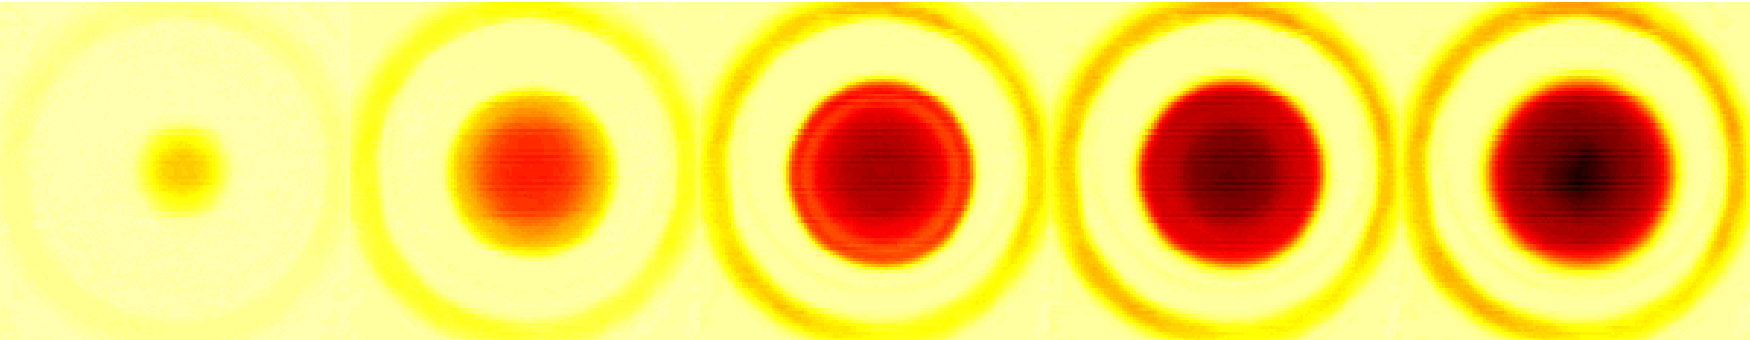
\includegraphics[width=1\linewidth]{Cover/coverimage}  \end{center} % gráficos
 \vspace{5mm}
\centering
\LARGE \textbf{Thermographical analysis of interface heat transfer mechanisms, with high temporal resolution}
%\\ \vspace{10mm}
%\Large Subtitle
\\ \vspace{15mm}
\Large \textbf{Pedro Daniel Fernandes Pontes} \\
\vspace{12mm}
\large Thesis to obtain the Master of Science Degree in
\\ \vspace{2mm}
\LARGE \textbf{Mechanical Engineering}
\\ \vspace{10mm}
\large Supervisors: Prof. Antonio Luís Nobre Moreira

Dr. Ana Sofia Oliveira Henriques Moita
\\ \vspace{15mm}
\Large \textbf{Examination Committee}
\\ \vspace{5mm}
\large Chairperson:	Prof. Viriato Sérgio de Almeida Semião \\
\large Supervisor: Dr. Ana Sofia Oliveira Henriques Moita \\
%\large Co-Supervisor: Prof. Lorem Ipsum \\
\large Member of the Committe: Prof. Edgar Caetano Fernandes \\
% Prof. Lorem Ipsum
 
\vspace{15mm}

%\Large \textbf{\todaythesis\today} \\
\Large \textbf{November 2016} \\
\let\thepage\relax
\end{flushleft}
\pagebreak


\clearpage
% Since I am using double sided pages, the second page should be white.
% Remember that when delivering the dissertation, IST requires for the cover to appear twice.

\thispagestyle{empty}
\cleardoublepage

\setcounter{page}{1} \pagenumbering{roman}

\baselineskip 18pt % line spacing: -12pt for single spacing
                   %               -18pt for 1 1/2 spacing
                   %               -24pt for double spacingnts} 
\thispagestyle{empty}
\pdfbookmark{Acknowledgments}{Acknowledgments}

\begin{acknowledgments} 

First would like to thank IST for being my home and teaching me everything I needed to get this far. It has been truly amazing studying here and knowing so many inspiring teachers and so many brilliant colleagues.\\
\par A huge thank you goes to my supervisor and teacher Doctor Ana Moita, for introducing me to the experimental world as well as all the patience, support and time that she put into my work. I'd also like to thank Emanuele Teodori for answering to all my questions and guiding me through every decision, even when far away. I'd also like to thank my professor and co-supervisor Doctor António Moreira for having me in his laboratory team.\\
\par A big acknowledgment goes also to my laboratory mates who helped me in countless occasions and kept me motivated. I'd like to give a special thank you to all the boiling team that gave great input into my work.\\
\par I'd like to give a special thank you to Henrique Carvalho, for being my electronics consultant and Vasco Rodrigues for the mechanical piece he made for me. Without them this thesis would be a lot harder. To all my other friends that helped me and motivated me I'd also like to say thank you.\\
\par This work couldn't also be done without workshop professor Manuel Venes and his colleague welding professor, for helping me welding the blackbody. For the device's box I need to thank my good friend Paulo Belga. Also, for all the support and help, I need to thank João and Pedro from LTO.\\
\par Finally for the constant patience and support, I'd like to thank my family. And last but not least I'd like to thank my girlfriend, Tânia for keeping me company during my writing sessions but mostly for all the love and support.

% Agradece tb por cortesia ao Prof Moreira, por te ter recebido na equipa do laboratório e na qualidade de teu co-orientador (por questões burocraticas)%
\end{acknowledgments}

% \hbox{} \vfill
% \begin{flushright}
% \small \textit{\textbf{"Try not to become a person of success, but rather try to become a person of value."}} %%% MUDAR %%%
% \\ \vspace{2mm}  
% \scriptsize Albert Einstein
% \end{flushright}

\clearpage
\thispagestyle{empty}
\cleardoublepage
%\input{0.Inicio/3.Acknowledgments.tex}
\selectlanguage{english}
\begin{abstract}
\par Interfacial heat transfer problems are present in various practical situations, including cooling applications. The accurate description of the observed phenomena, required to improve interfacial heat transfer requires accurate diagnostic techniques with high temporal and spatial resolution.

\par Time resolved Thermography has shown high potential to be used but requires a proper camera calibration. Care must be also taken in the post-processing procedure.

\par The present work explores time resolved infrared thermography, combined with high-speed imaging to describe the interface heat phenomena occurring during droplet impacts on heated surfaces, addressing the effect of different parameters such as wettability, impact velocity and liquid properties (surface tension). To comply with the demanded resolution a calibration was designed to improve the camera's precision. Several data processing techniques were also applied to extract the results and improve their quality.

\par Infrared thermography has allowed identifying and describing in detail particular phenomena reported in the literature. The proposed calibration improved the complaisance of the results with the expected heat transfer events. The results show that higher impact velocity, good wettability and low surface tension increase the heat flux between the surface and the impacting droplet. This was also related with the wetted area. The heat flux and cooling effectiveness calculated showed satisfactory values in accordance to the results previously reported in the literature.

\end{abstract}
\begin{keywords}
Infrared Thermography, Droplet Impact, Wettability, High-speed Imaging, Interfacial Phenomena, Heat Transfer.
\end{keywords}
\clearpage
\thispagestyle{empty}
\cleardoublepage
\selectlanguage{portuguese}
\begin{resumo}

\par Podemos encontrar, em várias aplicações práticas incluindo o arrefecimento, problemas de transferência de calor. É necessário uma caracterização precisa dos fenómenos observados para se melhorar a transferência de calor em interfaces, que requer técnicas de diagnostico com elevada resolução temporal e espacial.

\par A Termografia tem mostrado um grande potencial, mas necessita de uma calibração decente. Deve-se também dar especial atenção aos procedimentos de pós-processamento.

\par O trabalho aqui apresentado explora a combinação entre termografia de infravermelhos com elevada resolução temporal e imagiologia de alta velocidade para descrever os fenómenos de transferência de calor que ocorrem na interface durante impactos de gotas em superfícies aquecidas, analisando o efeito de diferentes parâmetros como a molhabilidade, velocidade de impacto e as propriedades dos líquidos (tensão superficial). Para satisfazer a necessidade de uma boa resolução, uma técnica de calibração foi desenhada para melhorar a precisão da câmara. Várias técnicas de pós-processamento foram também usadas para extrair resultados e melhorar a sua qualidade. 

\par A Termografia de Infravermelhos permitiu identificar e descrever em detalhe acontecimentos particulares que foram mencionados na literatura. A calibração proposta melhorou a complacência dos resultados extraído com os fenómenos de transferência de calor. Os resultados mostram que elevada velocidade de impacto, boa molhabilidade e baixa tensão superficial aumentam o fluxo de calor entre a superfície e a gota. Estas conclusões foram também relacionadas com a área molhada pela gota. O fluxo de calor e a eficácia de arrefecimento calculados mostram resultados que estão de acordo com o esperado na literatura.

\end{resumo}
\begin{palavraschave}
Termografia de Infra Vermelhos, Impacto de Gotas, Molhabilidade, Camâra de Alta Velocidade, Transferência de calor na Interface
\end{palavraschave}
\clearpage
\thispagestyle{empty}
\cleardoublepage
%% Use Main document Language
\selectlanguage{english}
%% ------
% This is required for the fancy chapters
\dominitoc
\dominilof
\dominilot

%%%%%%%%%%%%%%%%%%%%%%%%%%%%%%%%%%%%%%%%%%%%%%%%%%%%%%%%%%%%%%%%%%%%%%
% List of contents
%\renewcommand{\baselinestretch}{1}
\pdfbookmark[0]{Index}{index}
\pdfbookmark[1]{Contents}{toc}
\tableofcontents
% \contentsline{chapter}{References}{\pageref{bib}}
\clearpage
\thispagestyle{empty}
\cleardoublepage
%\renewcommand{\baselinestretch}{1.5}
%%%%%%%%%%%%%%%%%%%%%%%%%%%%%%%%%%%%%%%%%%%%%%%%%%%%%%%%%%%%%%%%%%%%%%
% List of figures
\pdfbookmark[1]{List of Figures}{lof}
\listoffigures
\clearpage
\thispagestyle{empty}
\cleardoublepage

%%%%%%%%%%%%%%%%%%%%%%%%%%%%%%%%%%%%%%%%%%%%%%%%%%%%%%%%%%%%%%%%%%%%%%
% List of tables
\pdfbookmark[1]{List of Tables}{lot}
\listoftables
\clearpage
\thispagestyle{empty}
\cleardoublepage

% %%%%%%%%%%%%%%%%%%%%%%%%%%%%%%%%%%%%%%%%%%%%%%%%%%%%%%%%%%%%%%%%%%%%%%
% % List of algorithms
% Requires packages algorithmic, algorithm
% \pdfbookmark[1]{List of Algorithms}{loa}
% \listofalgorithms
% \cleardoublepage
\acresetall
%% Remain list of table titles are set manualy
% %%%%%%%%%%%%%%%%%%%%%%%%%%%%%%%%%%%%%%%%%%%%%%%%%%%%%%%%%%%%%%%%%%%%%%
 % List of acronyms
\pdfbookmark[1]{List of Acronyms}{loac}

\chapter*{Abbreviations}


% See more at http://staff.science.uva.nl/~polko/HOWTO/LATEX/acronym.html

\begin{tabular}{ll}
IR   & Infra-red                        \\
\\
PIV  & Particle Image Velocimetry       \\
\\
PID  & Potential-Integrative-Derivative \\
\\
MW   & Mid Wavelength                   \\
\\
LW   & Low Wavelength                   \\
\\
MWIR & Mid Wavelength Infrared          \\
\\
ADU  & Analog to Digital Units     \\
\\
fps  & Frames per second     
\end{tabular}

\clearpage
\thispagestyle{empty}
\cleardoublepage




%%%%%%%%%%%%%%%%%%%%%%%%%%%%%%%%%%%%%%%%%%%%%%%%%%%%%%%%%%%%%%%%%%%%%%
% List of symbols
\pdfbookmark[1]{List of Symbols}{los}

\listofsymbols
\begin{table}[H]
\begin{tabular}{@{}p{1.7cm}@{}p{8cm}l}
\multicolumn{2}{l} {\textbf{Roman symbols}} \\ & \\
$W$   & Radiated Energy                     &  $W/m^2$ \\
$T$  & Temperature &  $K$ \\
$A$  & Area    & $m^2$  \\
$R_f$  & Relation between the surface area and its flat projected area & -  \\
$f$  & Fraction   &   -\\
$t$  & Time & $s$  \\
$r$  & Radius of the droplet & $m$  \\
$u$  & Velocity &  $m/s$ \\
$k$  & Conductivity &  $W/(mK)$ \\
$q''$  & Heat Flux  & $W/m^2$  \\
$c_p$  & Thermal capacity  &  $J/(kgK)$ \\
$P$  & Power  & $W$  \\
$Q$  & Heat Energy  & $J$  \\
$m$  & Mass  & $kg$  \\
$avTemp$  & Average Temperature  & $ºC$  \\
$vid$  & Pixel/Frames video matrix  & $kg$  \\
$x$  & Cartesian coordinate  & $m$  \\
$y$  & Cartesian coordinate  & $m$  \\
\end{tabular}
\end{table}

\begin{table}[H]
\begin{tabular}{@{}p{1.7cm}@{}p{8cm}l}
\multicolumn{2}{l} {\textbf{Greek symbols}} \\ & \\
$\alpha$  & Absorptivity     & -  \\
$\rho$  & Reflectivity & -  \\
$\tau$   & Transmissivity              & -  \\
$\varepsilon$  & Emissivity                & -  \\
$\lambda$ & Wavelength      &  $m$ \\
$\delta$  & Thickness of the foil &  $m$ \\
$\epsilon$  & Cooling Effectiveness  &  - \\
$\sigma_{SB}$  & Stefan-Boltzmann constant   & $5.67 \times 10^-8 \; W/(m^2K^4)$  \\
$\theta$  & Contact Angle   & degree  \\
$\sigma$  & Surface Tension   & $N/m$  \\
$\phi$  & Cylindrical coordinate  & degree  \\
$\beta$ & Spreading Factor & - \\
\end{tabular}
\end{table}


\clearpage
\thispagestyle{empty}

\cleardoublepage
% Pages number is starting now with arabic style... until now it was on roman mode
\pagenumbering{arabic} \setcounter{page}{1}
\baselineskip 18pt
%% Use Main document Language
\selectlanguage{english}
%% Define the title of Chapter Table of Contents
\mtcsettitle{minitoc}{Contents}
%% ------
\pagestyle{documentsimple}%Simple head
% %%%%%%%%%%%%%%%%%%%%%%%%%%%%%%%%%%%%%%%%%%%%%%%%%%%%%%%%%%%%%%%%%%%%%%
% The Introduction:
% %%%%%%%%%%%%%%%%%%%%%%%%%%%%%%%%%%%%%%%%%%%%%%%%%%%%%%%%%%%%%%%%%%%%%%
\chapter{Introduction}
\label{cap:int}

\section{Motivation}
\label{sec:int_motivation}
% bastante alterado

\par Heat transfer in fluid-solid interfaces, with fluid phase change is a common phenomenon observed  in the nature and relevant for a wide number of industrial applications, namely in cooling systems, based for instance in droplet/spray impact, or pool boiling. The heat transfer mechanisms occurring in such applications are complex and there are still several processes which remain unexplained, despite the numerous studies that have been reported in the literature.\\

\par The accurate description of such phenomena requires the use of diagnostic techniques with high spatial and temporal resolution has they occur in characteristic spatial scales which can be of the order of the micrometers and temporal scales of the order of milliseconds. Within this scope, several diagnostic techniques have been explored although many of them are intrusive and do not comply with the required spatial and temporal resolutions. For instance, the use of a thermocouples is a really common method, but is  intrusive to the measured process, can only measure the surface temperature at one specific location (one point) and cannot be in contact with electrically conductive means. With this in mind, infra-red (IR) thermography has been recently explored as a high potential alternative to some of the existing intrusive temperature measuring methods. A thermographic camera with a proper calibration can give high precision temperature results at high frame rates, which can provide high definition qualitatively and, more importantly, quantitatively accurate thermal images. The IR camera also outputs two dimensional images, a great advantage when trying to understand this kinds of processes, which are usually not restricted to a one dimensional analysis. \\ 

\par However, care must be taken when developing the calibration process and post-processing procedures, as there are many issues that must be considered, related to the dependence of the read temperature values with many parameters (e.g. ambient temperature, effect of the surroundings, surface emissivity, among others). Hence, custom made calibration and post-processing procedures must be developed and explored, to infer, based on a critical analysis, on the accuracy of the provided information and how useful it is to determine additional important features such as accurate temperature distributions, heat fluxes or cooling effectiveness.\\

\par In this context, the present work explores the use of time resolved infrared thermography to describe the heat transfer processes occurring at droplet impacts onto thin metal foils. Although the IR camera use will be centered in the boiling process, the heat transfer mechanisms in droplet surface impact will also be studied.\\

\par While this work was being developed, a complementary computational study is being performed by  Emanuele Teodori, so the results produced in the present work will also be used to validate the computational model that is being devised.
\section{State of The Art}
\label{sec:int_state}
\subsection{Infrared Thermography Techniques}
\par Starting by its discovery, infrared radiation was first reported by Hershel's famous experiment with a prism that would decompose the solar light. Frederick William Hershel noticed that when he placed a thermometer outside the visible spectrum, its temperature would still increase and deducted the existence of invisible radiation. The first patent of a radiation based thermometer was emitted in the end of the 19th century \cite{DeWitt1988}. Only after World War II a single point laser thermometer used in medicine, started being commercialized. Thermal cameras started being developed after the second World War, mainly for military purposes. A few years later IR systems would be used in various types of supersonic wind tunnels to detect aerodynamic heating. \\

%%% Czysz
\par In 1969, Czysz and Dixon \cite{Dixon1969} proposed a thermographic method to gather quantitative results. They applied a Phosphors coating to the surface. This coating is very sensitive to temperature. They placed heat sensors in key spots. The next step would be to use an Isodensitracer, a device that would read the density of the coating, make a density map (with iso-lines) and attribute a measured heat flux to each density level. They concluded stating that the key to gathering good quantitative results was to perform a good calibration. \\
%%% Sargent 
\par Inspired by Czysz and Dixon's work, in 1998, Sargent \textit{et al.} \cite{Sargent1998} followed the same approach and decided to use an IR camera to measure heat transfer in complex flows. Their calibration consisted in placing several thermocouples in their target surface. This calibration is often called \textit{in situ} calibration, for being made in the measured body. After collecting the video tape from the camera and post-processing it in the computer these authors correlated the grey scale values of the image with the temperatures measured by the sensors. The result can be seen in Figure \ref{fig:sargent}. This figure also shows the fitting curves, usually polynomials of second and third order. Czysz and Dixon \cite{Dixon1969} concluded that IR Cameras had a strong potential to be used in fluid dynamics measurements. They also concluded that \textit{in situ } calibrations can be very useful as they eliminate the need to calculate emissivity. \\

\begin{figure}
\centering
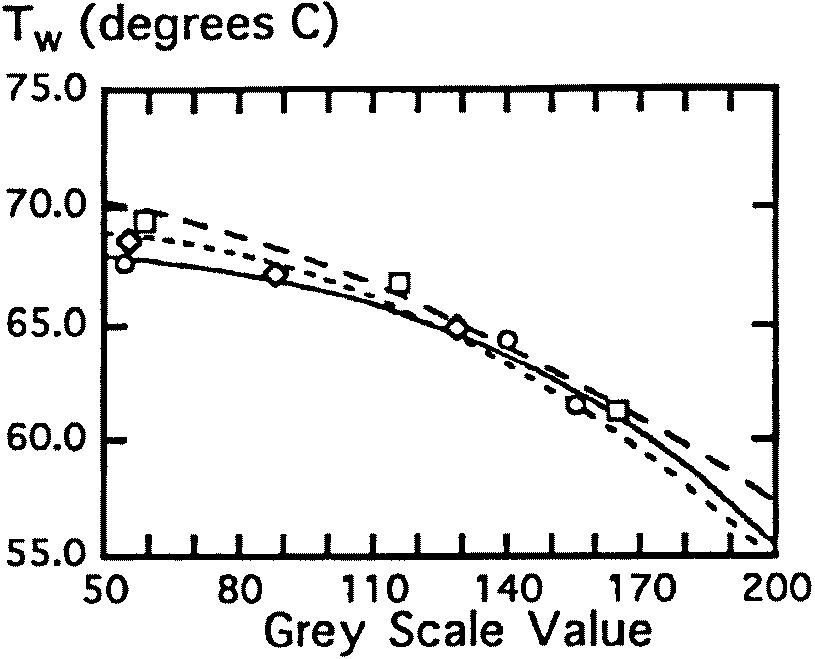
\includegraphics[width=0.5\linewidth]{Figures/1.Chapter/sargent.png}
\caption{Calibration of an IR Camera with polynomial fit}
\source{Sargent, 1998 \cite{Sargent1998}}
\label{fig:sargent} 
\end{figure}

%% Schwabe
\par In 2003, Schwabe \textit{et al.} \cite{schwabe2003oscillatory} pioneered the study of interfacial phenomena with an IR Camera. The experiments consisted on a cold surface where water would condensate, then flow back into a gap through a channel, where it would evaporate again. This was a closed cycle, covered by heated walls and a window made of Zinc Sulfide, a material transparent to IR radiation. To avoid condensation on the glass, a heater was placed on its center. However, this heater was a big obstruction to the camera's top view. \\

%%%Shen

\par In 2008, Shen \textit{et al.} \cite{shen2010simultaneous} studied simultaneous droplet impact and its influence on heat transfer from different heated surfaces. The used technique consisted in placing a high-speed camera horizontally to the droplet impact area and a infrared camera bellow the studied surface. They addressed the influence of surface topography on the heat transfer processes and observed that nano-structured surfaces had a significant lower heat removal by the droplets, when compared to smooth surfaces. It was also observed that the spreading diameter would increase with the surface heating for the nano-structured surface, while evaporation time was reduced.\\


%%Gerardi
\par In 2008, Gerardi \textit{et al.} \cite{Gerardi2008} started using thermographic cameras to study heat transfer through the macro- and micro-layer boiling applications. They wanted to observe bubble formation and study heat transfer in the interface between the bubble and the heated surface. Bubble formation is a phenomena that occurs between a small time window. To achieve this a IR Camera with high temporal resolution was used alongside with a high speed camera. The bubble formation was observed from the bottom of the experimental setup. This could only be done with a dichroic beamsplitter, that transmits IR radiation to the IR camera and is transparent to the visible light. To allow the radiation to pass from the bubble, the heated surface had to be transparent to both visible and infrared spectra, so it was made of sapphire. The sapphire thin plate had also a deposited film so it could be heated by Joule effect. With this setup it was possible to observe heat removal from a bubble from a constant heat flux source as it departs, with elevated time precision. The fact that Gerardi \textit{et al.} \cite{Gerardi2008} were able to synchronize the frames of both the IR and the high speed cameras enabled them to put side by side the images of both cameras. Correspondence of temperature maps and the phases of bubble departure was made so that thermal and physical phenomena could be matched. \\

%%Tartarini
\par In 2009, Tartarini \textit{et al.} \cite{tartarini2009} crossed the study of droplet cooling with infrared thermography. While previous studies focused mainly on stable isothermal conditions, Tartarini \textit{et al.} decided to focus on the study of transient conditions. To do this, the authors chose to use a IR transparent slab, heated by two radiators. Again, the IR camera would be put under the droplet, that would collect data, which would be processed in MATLAB to remove noise and apply an emissivity map. Tartarini \textit{et al.} coated the surface with a high emissivity paint on its upper side. This procedure aimed at minimizing errors associated to emissivity and study more accurately the solid-fluid interface. The experimental data allowed these authors validating a numerical model to predict transient temperatures. It was also possible to observe temperature drop at the center of the droplet using a time-frame of a minute. \\

%%Girard
\par In 2010, Girard \textit{et al.} \cite{girard2010infrared} used thermography in order to study droplet evaporation. In this experiment, like the one of Tartarini \textit{et al.} made, the author used an elevated time-frame, but with a more fine temporal resolution. In this setup a droplet fell on a heated copper surface. The IR camera was placed on top of the droplet on this setup. The authors observed the evaporation time using different surface temperatures. They focused on the interface between the water droplet and copper surface that due to their different emissivity was pretty noticeable. Based on this, Girard \textit{et. al.} reported the interface temperature and droplet radius along the time. \\

%% Kim and Buongiorno
\par In 2011, Kim and Buongiorno \cite{kim2011detection} proceeded with the work started in 2008 by Gerardi \textit{et al.} and used thermography to detect the triple interface between solid-liquid-vapour in pool boiling with a similar setup. To detect this interface they used an optical silicon wafer (transparent to IR) in contrast with \cite{Gerardi2008} which used coated sapphire. The camera detected the bubbles as dark spots and the liquid as bright spots. In this work the different absorptivity and temperatures of the distinct phases were used to detect the triple contact-line. Kim and Buongiorno observed the formation of a microlayer, where the radiation from the vapor would cross the water, and an area where the radiation would come from the bubble. The frontier between was concluded to be the limit between these 2 regions. \\

%% Duan
\par In 2013 Duan \textit{et al.} \cite{duan2013synchronized} synchronized not only the high-speed camera with the IR camera, but also used Particle Image Velocimetry (PIV) data. The objective was studying bubble formation and departure in pool boiling. The approach to use the IR camera was similar to \cite{Gerardi2008} but the high speed camera was placed horizontally to the boiling cell. Glass windows were mounted all around the wall to enable side view. The PIV laser was placed in the window frontal to the high speed camera's window. These authors could observe a dependence of the interval between bubble departure and formation with temperature, a strong cooling underneath the bubble, due to the microlayer. The observation of micro scale phenomena was only possible only by combining the high-speed camera, the IR camera and PIV. \\

%% Sielaf

\par More recently (2014), Sielaf \cite{sielaff2014experimental} used a different technique to gather interface data from pool boiling. Sielaf used a thin stainless steel foil under a heater. Given the small thickness of the foil, the interface temperature on top of the foil would be very close to that of the bottom surface. Sielaf also used a calibration technique close to the \textit{in situ} approach. With a thermocouple inside is pool boiling cell, near the foil and with the very close assumption that the foil would be at the same temperature, each pixel was calibrated for that temperature. Additional noise filters were applied in the post processing. As many of previously mentioned authors, Sielaf used the high-speed camera horizontally to his boiling cell. Another characteristic of his technique was that the foils enabled him to identify the transition from the contact line to a microlayer. Sielaf identified that this transition occurs during the receding phase of the bubble. \\

%% Zupancic
\par Additional studies using a thin foil have been performed in the past year. For instance, in 2015 Zupancic \textit{et al.} used this approach while also applying different coatings to study different wettability regimes. In this study, the heating of the foil is made directly by Joule effect with copper contacts on the foil. In 2016 Petkovsek \textit{et al.} observed, with a similar setup the hot spot phenomena. In this hot spot, measured temperature would be higher than the surroundings. \\

\subsection{Numerical Studies}

\par In this section some relevant numerical work about heat transfer in droplet impact will be discussed. This work contributed aswell to better understanding droplet related phenomena and heat transfer.\\
\par Numerous numerical droplet simulations have been performed in the last century, but the assumptions made to simplify them were questioned by several authors such as Healy \textit{et al.} \cite{healy2001validity} in 2001. Heat transfer during the spreading phase had been neglected, for representing a small fraction of the evaporation time. Although it seems a reasonable assumption, Healy \textit{et al.} found that in the spreading phase, the droplet temperature raise caused an alteration of its properties which resulted in significant errors. Still in 2001, Pasandideh-Fard \textit{et al.} \cite{pasandideh2001cooling} tested a numerical model that studied heat extraction, comparing it between impact velocities. Besides validating the model, impact velocity had a weak effect on the calculated temperature variation and heat flux. The principal effect of the increase of this parameter is that more area is wetted which means that extracts heat from a greater area. Later in 2010, Strotos \textit{et al.} \cite{strotos2011non} was able to identify, in his numerical work, various phenomena such as the bubble trapping effect and the neck in the droplet's lamela, and the heat transfer effects that these phenomena cause. In the case of the bubble trapping effect, an increase of the temperature in the droplet center, in the first moments after the impact was noted. In the case of the lamela neck a relation was made between its formation and position and an increase of temperature in that area.



\section{Objectives}
\label{sec:int_contributions}

\par The main objective of this work is to explore the potential of the use of an high speed infrared camera to study in detail the heat transfer processes occurring at liquid-solid interfaces.\\

\par Here, the proper calibration and post-processing procedures must be developed and tested on a case study. Which was chosen to be the impact of droplets onto heated thin foil surfaces.\\

\par The IR images are analyzed together with high speed images, to relate droplet dynamics with heat transfer processes.\\

\par The calibration and post-processing procedures developed are evaluated based on a critical analysis to infer on how good the data collected by the IR camera can be used to describe in detail the phenomena reported in the literature and provide complementary information on the temperature distributions, heat flux and cooling effectiveness
Finally, the validated data is also used to explore the physics governing the observed phenomena and discuss the effect of droplet impact velocity, wettability, liquid surface tension and temperature.\\

\par The heat transfer processes occur at single phase and when the liquid droplet is boiling.

\section{Thesis Outline}
\label{sec:int_outline}

\par The present dissertation is organized in 6 main chapters including this introductory section that provides the motivation of the work, a state of art to contextualize the work and the main objectives to achieve.\\

\par The main concepts and theoretical background required to better understand the procedures developed in Chapter 4 and the results discussed in Chapter 5 are presented in Chapter 2.\\

\par Chapter 3 describes the experimental setups and measured procedures followed. The functioning of the IR camera and the software calibration methods are discussed here.\\

\par One of the most important parts of the work is the calibration and post process methods that are proposed in the work. These methods are explained in detail in Chapter 4, against the methods available in the camera software.\\

\par The results are presented and discussed in chapter 5.\\

\par Finally, chapter 6 draws the main conclusions and provides several recommendations to be considered in future work.


\cleardoublepage
% %%%%%%%%%%%%%%%%%%%%%%%%%%%%%%%%%%%%%%%%%%%%%%%%%%%%%%%%%%%%%%%%%%%%%%
% Dummy Chapter:
% %%%%%%%%%%%%%%%%%%%%%%%%%%%%%%%%%%%%%%%%%%%%%%%%%%%%%%%%%%%%%%%%%%%%%%

% %%%%%%%%%%%%%%%%%%%%%%%%%%%%%%%%%%%%%%%%%%%%%%%%%%%%%%%%%%%%%%%%%%%%%%
% The Introduction:
% %%%%%%%%%%%%%%%%%%%%%%%%%%%%%%%%%%%%%%%%%%%%%%%%%%%%%%%%%%%%%%%%%%%%%%
\chapter{Theoretical Background}
\label{cap:theoretical}

%\textit{In this chapter some theoretical background will be given about what's going to be discussed further.}

\section{Infrared Thermography}
\label{sec:sectiona}

Heat transfer through radiation is the way, in thermography, most often used to gather quantitative information on surface temperature. One of the main objectives of this work is to correctly convert the measured radiation intensity plus the information on the body emissivity and surrounding conditions in an accurate temperature estimate. To do so, some theoretical notions must be introduced.

\subsection{Radiation Intensity to Temperature Conversion}
\label{subsec:rad2tem}

Radiation is emitted by all bodies at $T>0 K$. The intensity of this radiation largely depends on the direction, wavelength and of course temperatures. For example, above 500ºC, a body's radiation is almost entirely in the IR wavelength \cite{IRCAM}. Besides emitting radiation a body can also absorb ($\alpha$), reflect ($\rho$) and radiation can even pass through it ($\tau$). Adding all this elements we get the Total Radiation Law:
\begin{equation}\label{eq:w}
    W = W\alpha + W\rho + W\tau
\end{equation}
in which $W$ represents the total energy transmitted through radiation. Equation \ref{eq:w} can be simplified as:
\begin{equation}\label{eq:1}
	1 = \alpha + \rho + \tau
\end{equation}
Note that in the equation \ref{eq:1}, $\alpha$, $\rho$ and $\tau$ represent the respective absorbed, reflected and transmitted fractions of the incident radiation energy, and have values between 0 and 1.\\

\subsubsection{Blackbody Equations}

\par One of the most important concepts that is used in this work is the concept of \textit{blackbody}. A \textit{blackbody} is characterized for absorbing all energy transmitted through radiation. In the ideal case of a \textit{blackbody} the coefficients assume the following values: $\alpha=1, \ \rho=0, \ \tau=0$. The blackbody is also a perfect emitter. The emissivity ($\varepsilon$) of a body characterizes the efficiency of a body for emitting energy, so it's the ratio between the energy emitted and the energy emitted if the body was a \textit{blackbody}. With this in mind one can use the equation \ref{eq:2} for a \textit{blackbody}. This equation is called Kirchhoff Law. Kirchhoff Law is also applied for the same wavelength ($\lambda$) so one can also use equation \ref{eq:3}.

\begin{equation}\label{eq:2}
\alpha=\varepsilon
\end{equation}
\begin{equation}\label{eq:3}
\alpha(\lambda)=\varepsilon(\lambda)
\end{equation}
\par For the specific case of a \textit{blackbody} one can also apply equation \ref{eq:4}. This equation is called Stefan-Boltzmann law and it states the relation between energy emitted through radiation and the temperature of the body. If the body is not perfectly black, but it's absorption/reflection/transparency properties don't vary with the wavelength, it's called as \textit{greybody} and in this case one should use Equation \ref{eq:5}.
\begin{equation}\label{eq:4}
W=\sigma_{SB} T^4
\end{equation}
\begin{equation}\label{eq:5}
W=\varepsilon \sigma_{SB} T^4
\end{equation}
where $\sigma_{SB}=5.670373 \times 10^8 W m^{-2} K^{-4}$ is the Stefan-Boltzmann constant.\\
\par It's fairly obvious these are concepts that illustrate ideal situations, and even though in most experiments shown further ahead the materials are chosen to be as close to \textit{black} or \textit{greybodies}, those aren't perfect. Of course this is attenuated by the fact that thermography measures in small intervals of wavelength. The next subsection will relate how a wavelength interval is selected, and it's relation with the atmosphere.

\subsubsection{Atmosphere Attenuation}
\label{subsec:atmat}

\par Almost every thermographical camera is separated from its target by the atmosphere, which has good or bad transmittance in different wavelengths. The atmosphere attenuation depends on the complexity of it's composition. For example, each of the following molecules: $H_2O$, $O_2$, $CO_2$ have certain wavelength values for which $\tau=0$. This means that in these wavelengths IR radiation will not pass through the atmosphere and its intensity cannot be measured.\\


\begin{figure}[h]
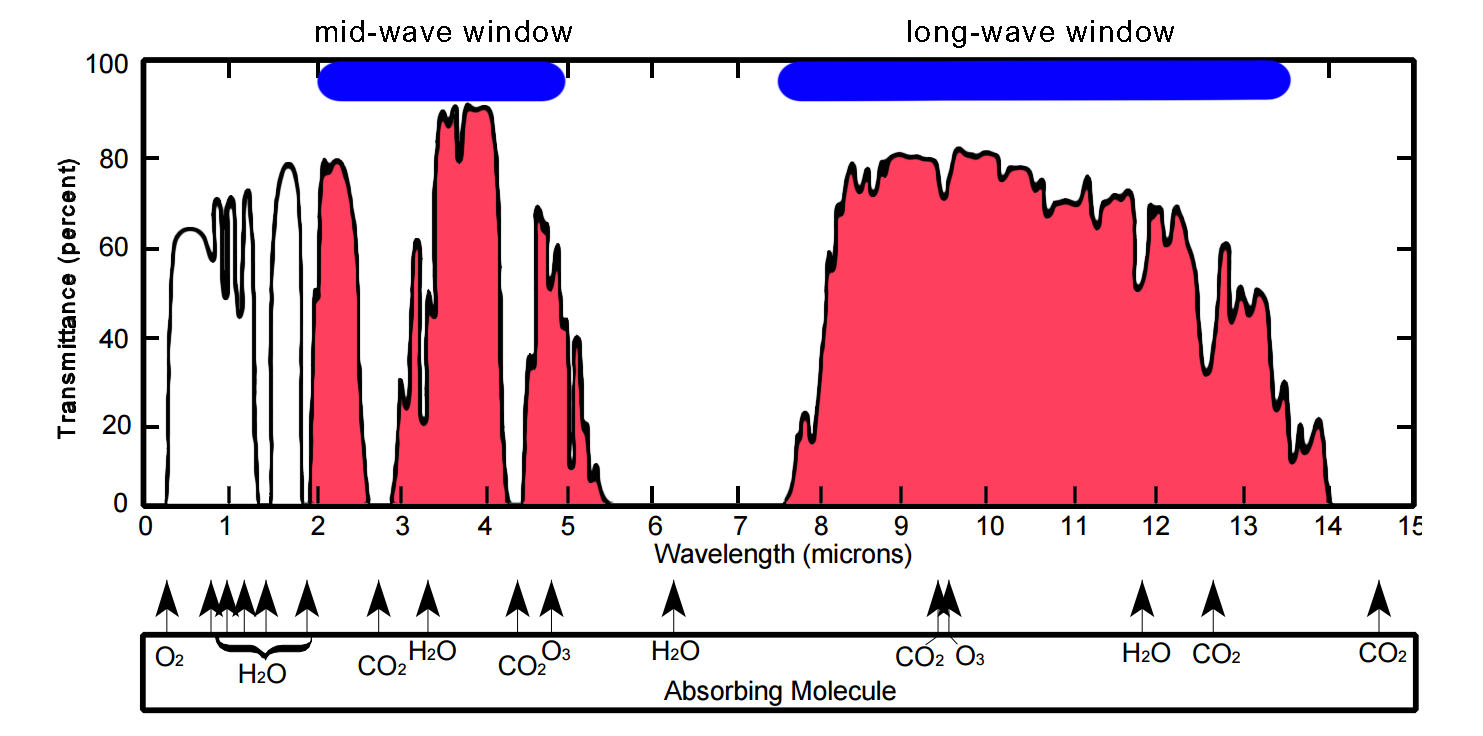
\includegraphics[width=1\linewidth]{Figures/2.Chapter/atmospheric_window.png}
\caption{Atmospheric Windows}
\source{Adaptation from chapter 7's Figure 10 of \cite{desk1997electronic}}
\label{fig:atm}
\end{figure}

\par This issue calls requires of choosing a wavelength \textit{window} for which the transmittance is close to 1. These \textit{windows} can be seen in Figure \ref{fig:atm}. It is possible to identify 2 main regions: the medium-wave \textit{window} (from 2-5 $m \mu$), or MW, and the long-wave \textit{window} (from 7.5-13.5 $m \mu$), or LW. The used camera works in the MW range so a selective range of wavelength inside it had to be chosen to avoid "bad atmosphere transmittance".\\

\subsubsection{Total Radiation}
\par When measuring a body's temperature with the IR Camera, there are other radiation sources that have to be accounted for. In total one can divide these radiation sources in 3 categories, shown bellow:
\begin{itemize}
\item The radiation emitted by the object/objects of study
\begin{equation}
W_{obj}=\varepsilon_{obj} \ \sigma_{SB} \ T_{obj}^4
\end{equation}
\item The radiation emitted by the atmosphere (where $ \ \varepsilon_{atm}=1-\tau_{atm}$ because $\rho_{atm}~=0$)
\begin{equation}
W_{atm}= (1-\tau_{atm}) \ \sigma_{SB} \ T_{atm}^4
\end{equation}
\item The radiation from the surroundings reflected by the object/objects.
\end{itemize}
\begin{equation}
W_{refl}=(1-\varepsilon_{obj}) \ \sigma_{SB} \ T_{refl}^4
\end{equation}
where $T_{refl}$ refers to the apparent temperature of the surroundings radiating to the measured body.\\
\par Figure \ref{fig:camscheme} identifies these sources and their origin. Note all the expressions in the figure represent energy radiated. In it it's possible to observe that 2 sources of radiation come from the studied body and represent the emitted and reflected components. When these components cross the atmosphere, they are affected by its transmissivity, $\tau_{atm}$ (this value in common atmospheric conditions is close to 1). The atmosphere itself can emit radiation, but because $\tau_{atm}$ is so close to 1, this is mostly negligible.\\

\begin{figure}
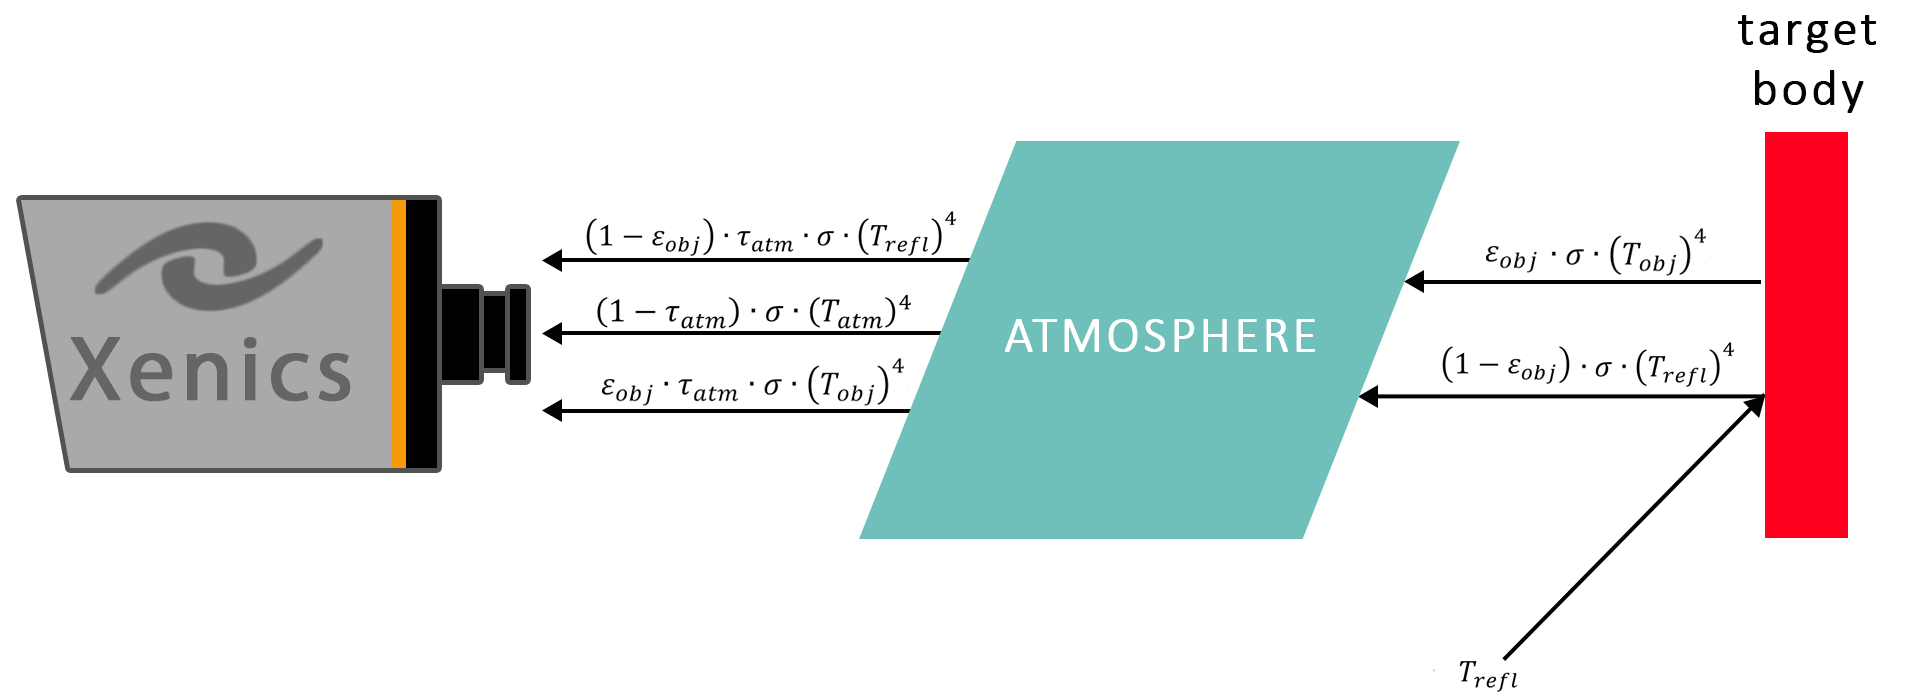
\includegraphics[width=1\linewidth]{Figures/2.Chapter/ir_camera_radiation_scheme.png}
\caption{Total radiation sources scheme}
\label{fig:camscheme}
\end{figure}

\par With these equations it is possible to relate the radiated energy received $W$ and the body temperature. This relation is seen in equations \ref{eq:6} and \ref{eq:7}.
\begin{equation}\label{eq:6}
W_{tot}=W_{obj}+W_{refl}+W_{atm}=(\varepsilon_{obj} \ \sigma_{SB} \ T_{obj}^4)+((1-\varepsilon_{obj}) \ \sigma_{SB} \ T_{refl}^4)+((1-\tau_{atm}) \ \sigma_{SB} \ T_{atm}^4)
\end{equation}
\begin{equation}\label{eq:7}
T_{obj}=\sqrt[4]{\frac{W_{tot}-(1-\varepsilon_{obj}) \ \sigma_{SB} \ T_{refl}^4-(1-\tau_{atm}) \ \sigma_{SB} \ T_{atm}^4}{\sigma_{SB} \ \varepsilon_{obj}}}
\end{equation}
\par The camera receives the total radiation $W_{tot}$, and the user has to input the emissivity and both the ambient and reflection temperatures in the camera software.

\section{Wettability}

\par Wettability is quantified by how well the surface is wetted by a liquid. This property is often characterized based on the equilibrium contact angle of a droplet deposited on a sold surface. This angle is given by the balance of the interface tensions acting between the surface, liquid and the vapor surroundings. The balance between these tensions is represented in Figure \ref{fig:tensao}
\begin{figure}[h]
\centering
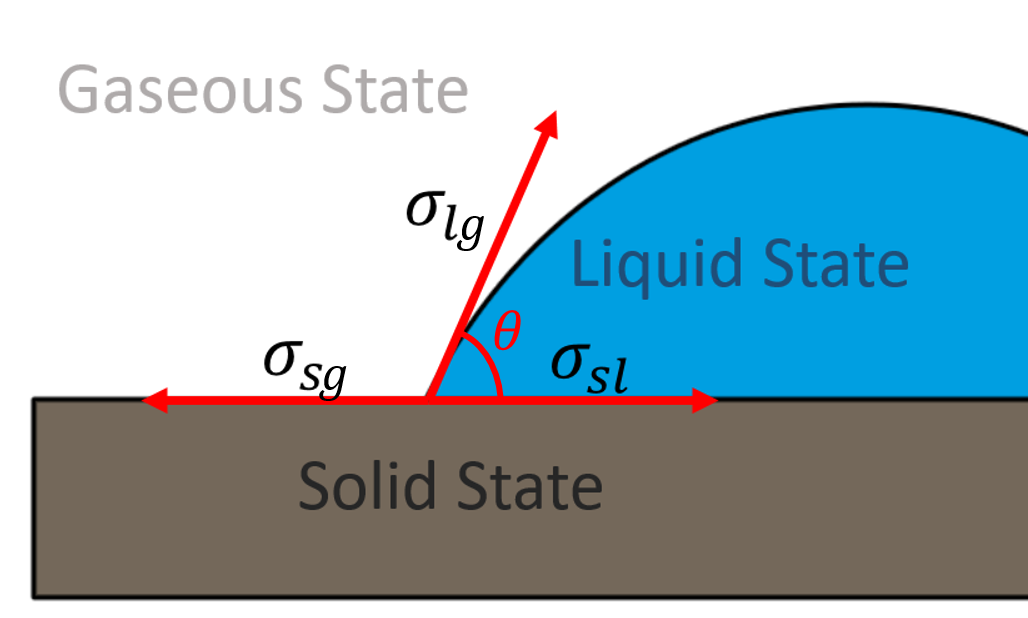
\includegraphics[width=0.5\linewidth]{Figures/2.Chapter/tensao.PNG}
\caption{Tension Balance}
\label{fig:tensao}
\end{figure}
\par From a thermodynamics perspective, the equilibrium condition of a liquid droplet are calculated by the minimization of the Gibbs energy of the system, G. When one considers constant temperature and pressure conditions it is possible to derive the well known Young's equation \cite{young1805essay} from this minimization ($dG=0$), which is simply the aforementioned balance of the interface tensions in the horizontal axis:
\begin{equation}
\sigma_{sg}=\sigma_{sl}+\sigma_{lg}cos(\theta_e)
\end{equation}
where $\sigma$ represents the interface tension at the solid-liquid (sl), solid-gaseous (sg) and liquid-gaseous (lg) boundaries and $\theta_e$ represents the equilibrium contact angle. High wettability droplet-surface-surrounding systems have $0\si{\degree} <\theta_e<90\si{\degree} $ and low wettability have $90\si{\degree}<\theta_e<180\si{\degree} $. The perfect wetted system has $\theta=0\si{\degree} $ and the perfect non-wetted system has $\theta=180\si{\degree} $ \cite{choi2011wettability}. If the liquid in study is water, the well wetted surfaces are called hydrophilic, while poor wetted surfaces are hydrophobic. Since ideal wetting/non-wetting situations do not exist, several authors (e.g. Koch \textit{et. al.} \cite{koch2009superhydrophobic}) consider the concept of superhydrophilic in $\theta_e<10\si{\degree}$ and superhydrophobic surfaces $\theta_e>150\si{\degree}$ the latter must also depict low histeresis. These regimes are depicted in Figure \ref{fig:wet}.

\begin{figure}[h]
\centering
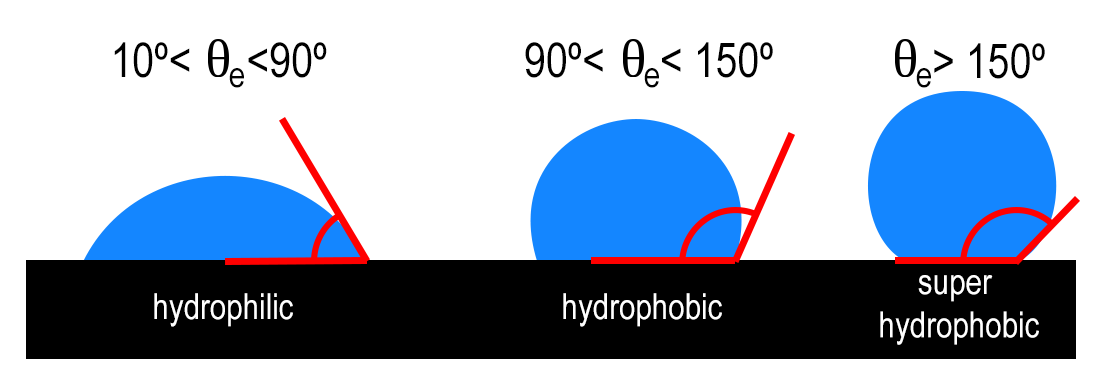
\includegraphics[width=0.7\linewidth]{Figures/2.Chapter/wet.png}
\caption{Wetting Regimes}
\label{fig:wet}
\end{figure}

\par While Young equation assumes that the surface is ideally smooth, in reality one has to take in account the roughness of the surface. Considering an rough homogeneous interface, one can convert the smooth surface contact angle ($\theta_e$) to the actual contact angle ($\theta$) using a formula based on the force balance and empirical correlations, presented in Equation \ref{eq:wenzel}. 
\begin{equation}\label{eq:wenzel}
cos \theta = R_f cos \theta_e
\end{equation}
where $R_f= \frac{A_{SL}}{A_{F}}$ is the relation between the surface area, to its flat projected area. This equation is called the Wenzel equation \cite{wenzel1936resistance}. Cassie took a different approach and considered an heterogeneous interface, where air would be trapped between the liquid and the surface, in pockets formed by the surface roughness. So having an interface with a fraction $f_1$ at one contact angle $\theta_1$ and another at $f_2$ and $\theta_2$, the contact angle would be given by Cassie's Equation \cite{cassie1944wettability} :
\begin{equation}\label{eq:cassie}
cos \theta = f_1 cos \theta_1 + f_2 cos \theta_2
\end{equation}
\par The difference between these two approaches can be seen in Figure \ref{fig:wenzelcassie}

\begin{figure}[h]
\centering
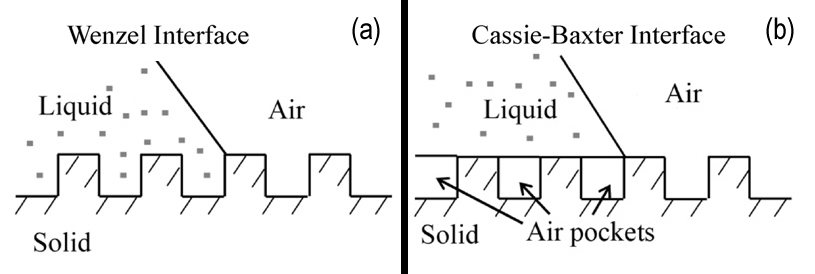
\includegraphics[width=0.7\linewidth]{Figures/2.Chapter/wenzelcassie.png}
\caption{Contact Angle approaches: (a) Wenzel, (b) Cassie-Baxter}
\source{Adapted from Bhushan, 2011\cite{bhushan2011natural}}
\label{fig:wenzelcassie}
\end{figure}


\section{Droplet Impact}

\par Several outcomes arrive from droplet impact, which depends on the impact conditions (size of the droplet and impact velocity), liquid properties and the boundary conditions established by the surface temperature and wettabillity:

\begin{itemize}
\item Rebound: after the impact the droplet bounces the surface partially or fully. Partial rebound happens when the surface is hydrophobic, while full rebound usually requires the surface to be super-hydrophobic.
\item Stick and Spread: the droplet sticks to the surface after the impact, spreading in the radial direction on the thin liquid film lamella. This is characteristic of hydrophilic surfaces.
\item Disintegration: the droplet sticks to the surface but smaller droplets are released in the spreading phase. Different disintegration mechanisms can be identified depending on the wettability, surface topography and impact conditions (Moita \textit{et. al.} \cite{moita2007drop}).
\end{itemize}

\par As the droplet hits the surface it deforms and spreads as a radial liquid film on the surface. The different outcomes arrive after this initial impact stage called as the kinematic phase.
As the liquid film (lamella) starts to form, the spreading velocity is dictated by the velocity of the contact edge of the film that instantly forms ($u_ce$). This parameter can be related with the droplet impact velocity($u_i$) and with the contact angle using \ref{eq:droplet}.
\begin{equation} \label{eq:droplet}
u_{ce}=\frac{u_i}{tan \theta}
\end{equation}

\par The lamella continues to spread governed by inertial effects until reaching its maximum diameter. Afterwards the lamella starts to recoil until reaching an equilibrium state.\\

\par While the earlier stages of spreading until reaching the maximum spreading diameter are governed by inertia, at the maximum spreading and at the recoiling phases viscous dissipation and wettability gain relative importance. Hence, spreading followed by recoiling is usually observed for impacts on hydrophilic surfaces, while rebound often occurs on hydrophobic surfaces, as the wettability precludes the contact between the lamella and the surface, lessening the viscous dissipation. Consequently, at the end of the recoiling phase the excess of surface energy is high enough to promote the droplet rebond from the surfaces. These phenomena are illustrated in figures 2.6 and 2.7.\\

\par To characterize the spreading and the recoiling phases many authors usually consider the spreading ratio $\beta(f) =\frac{D(t)}{d_0}$, which provides the temporal variation of the spreading diameter made non dimentional by the initial droplet diameter \cite{rein1993phenomena}. The time is also often made non dimensional as:

\begin{equation}\label{eq:rein}
t^*=\frac{t u_i}{r}
\end{equation}

where r is the droplet radius at that time.

\begin{figure}[h]
\centering
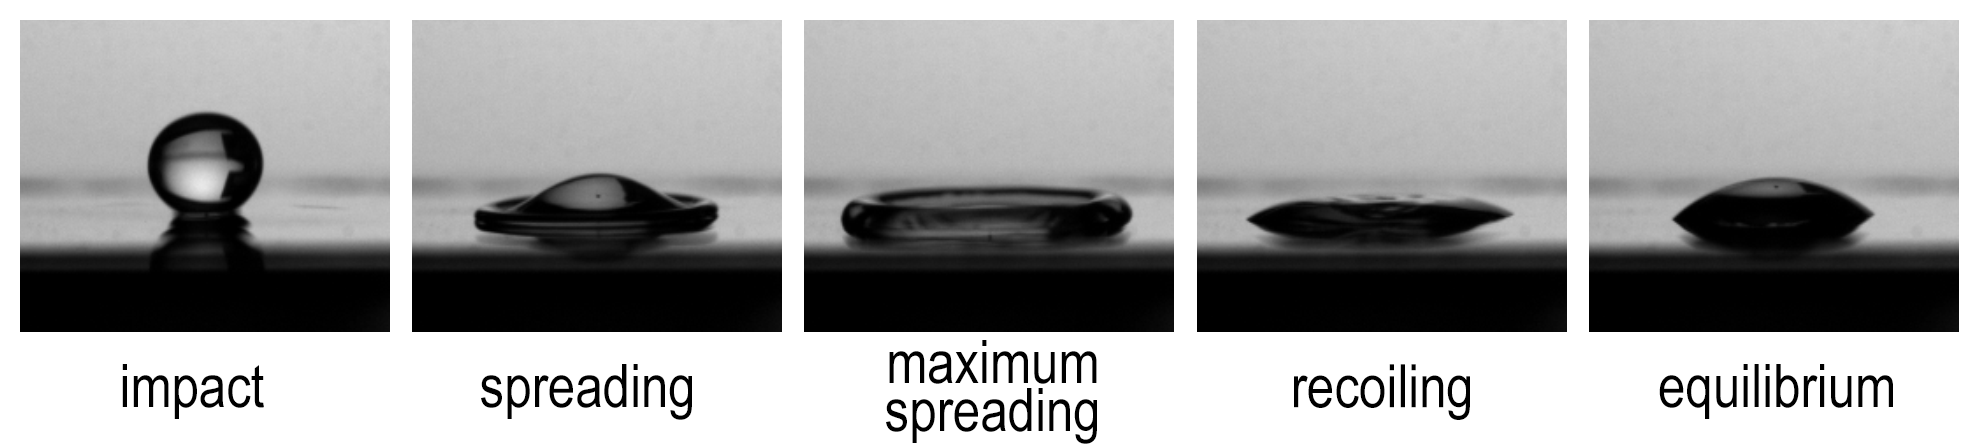
\includegraphics[width=0.9\linewidth]{Figures/2.Chapter/droplet.png}
\caption{Droplet impact stages, for an hydrophilic surface}
\label{fig:droplet}
\end{figure}

\begin{figure}[h]
\centering
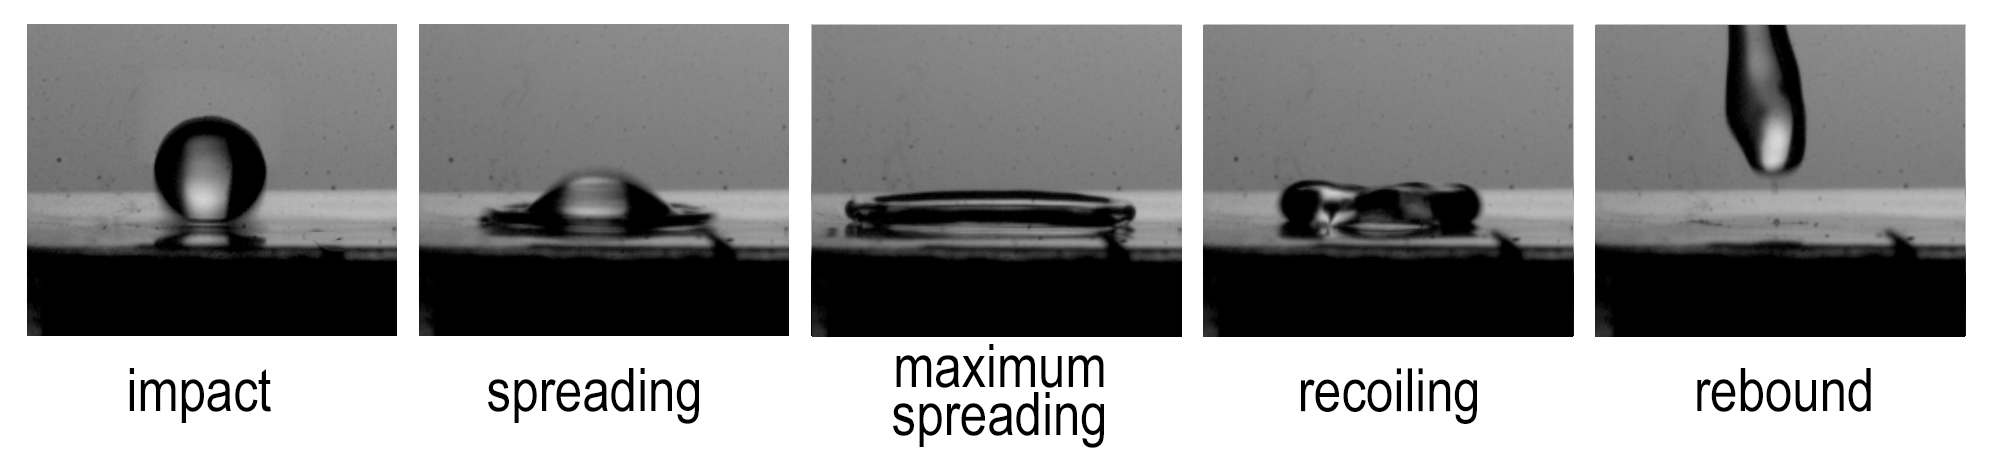
\includegraphics[width=0.9\linewidth]{Figures/2.Chapter/droplethf.png}
\caption{Droplet impact stages, for an hydrophobic surface}
\label{fig:droplethf}
\end{figure}

\section{Heat Transfer}
\label{sec:heat}

\par During droplet impact, the most important heat flux to evaluate is the change of heat between the droplet and the heater. According to \cite{sielaff2014experimental}, the heat flux from the droplet can be written as:

\begin{equation}\label{eq:heat}
q''=q_0''+k_h \delta (\frac{{\partial}^2 T}{\partial x^2}+\frac{{\partial}^2 T}{\partial y^2})-\rho_h c_{p,h} \delta \frac{{\partial} T}{\partial t} \quad [W/m^2]
\end{equation}

where $q_0$ is the heat flux from the heater, $k_h$, $\rho_h$ and $c_{p,h}$ are the conductivity, density and specific heat capacity of the heater's material and $\delta$ is the thickness of the heater. Across the radius of the droplet, the heat flux curves are similar to these reported by \cite{pasandideh2001cooling} and represented in Figure \ref{fig:fluxo}. High heat transfer occurs in the first instants after impact (t< 2 ms). As the droplet spreads a peak in the heat flux is observed at the edge of the lamela. This is due to "new" cold liquid reaching the hot surface. The heat flux is reduced substantially in time at later stages of spreading (t>4 ms), mainly because the droplet is heating and the liquid speed is decelerating, thus reducing convective and conductive heat transfer.

\begin{figure}[h]
\centering
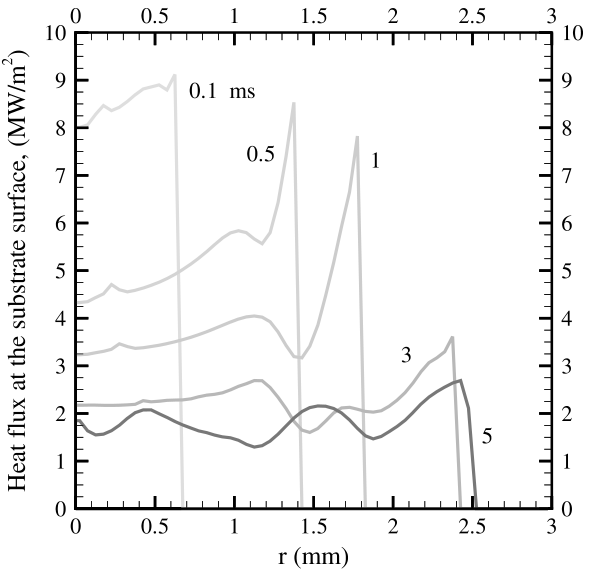
\includegraphics[width=0.5\linewidth]{Figures/2.Chapter/fluxo.png}
\caption {Heat Flux at the surface for different timesteps}
\label{fig:fluxo}
\source{M. Pasandideh-Fard, 2001 \cite{pasandideh2001cooling}}
\end{figure}

\par In the droplet case, the flux for various points along the radius is being analyzed, and this calculation is made using cylindrical coordinates and considering the temperature distribution to be axyssimetrical. To convert the coordinate system, one should first consider the following transformation of the second derivative:

\begin{equation}
\frac{\partial^2}{\partial x^2}=(cos \phi \frac{\partial}{\partial r} - \frac{sin \phi}{r}\frac{\partial}{\partial \phi})(cos \phi \frac{\partial}{\partial r} - \frac{sin \phi}{r}\frac{\partial}{\partial \phi})
\end{equation}

\begin{equation}
\frac{\partial^2}{\partial y^2}=(sin \phi \frac{\partial}{\partial r} - \frac{cos \phi}{r}\frac{\partial}{\partial \phi})(sin \phi \frac{\partial}{\partial r} - \frac{cos \phi}{r}\frac{\partial}{\partial \phi})
\end{equation}

\par Considering now the condition of axyssimetry ( $\frac{\partial}{\partial \phi}=0$), and applying the expression to the temperature field, one can write the sum of the second derivatives as:

\begin{equation} \label{eq:coord}
\frac{\partial^2 T}{\partial x^2}+\frac{\partial^2 T}{\partial y^2}=(cos^2 \phi \frac{\partial^2 T}{\partial r^2}) + (sin^2 \phi \frac{\partial^2 T}{\partial r^2})= (cos^2 \phi + sin^2 \phi )\frac{\partial^2 T}{\partial r^2} = \frac{\partial^2 T}{\partial r^2}
\end{equation}

\par Thus, the equation for the heat flux removed by the droplet, considering the axyssimetry condition, can be written as:

\begin{equation}\label{eq:heatf}
q''=q_0''+k_h \delta (\frac{{\partial}^2 T}{\partial r^2})-\rho_h c_{p,h} \delta \frac{{\partial} T}{\partial t} \quad [W/m^2]
\end{equation}

\par The power dissipated ($P_{diss}$) by the droplet is the integral of this expression in the droplet area, and it's given by:

\begin{equation}\label{eq:diss}
P_{diss}= \int_{A} q'' \; dA \quad [W]
\end{equation}

\par Since the droplet, ideally, is always axisymetric, it is necessary to decompose $dA$ in cylindrical coordinates. Equation \ref{eq:diss} is expressed in cylindrical coordinates in Equation \ref{eq:cyl}. Integrating the power in time one ends up with the total heat extracted. This is expressed in Equation \ref{eq:qtot}.

\begin{equation} \label{eq:cyl}
P_{diss} = \int_\theta \int_r r \, q'' \; dr d\phi \quad [W]
\end{equation}
\begin{equation} \label{eq:qtot}
Q_{tot} = \int_t P_{diss} \; dt [J]
\end{equation}

\par Pasandideh-Fard \cite{pasandideh2001cooling} proposed a way to quantify the "cooling effectiveness" ($\epsilon$) of the droplet. This effectiveness is described by the actual heat removed by the droplet divided by the maximum heat transfer possible be removed in theory (assuming no phase change). This coefficient is described by Equation \ref{eq:epsilon}.

\begin{equation}\label{eq:epsilon}
\epsilon= \frac{\int_t \int_A q'' \; dA \, dt}{(m c_p \Delta T)_{water}}
\end{equation}

\par The relation between the cooling effectiveness and the time adimensionalized for different impact velocities has been computed by \cite{pasandideh2001cooling} and is shown in Figure \ref{fig:cooling}. The cooling effectiveness grows with the impact velocity because, as shown in Equation \ref{eq:rein}, the spreading factor is larger, meaning that the area covered by the droplet also grows.

\begin{figure}[h]
\centering
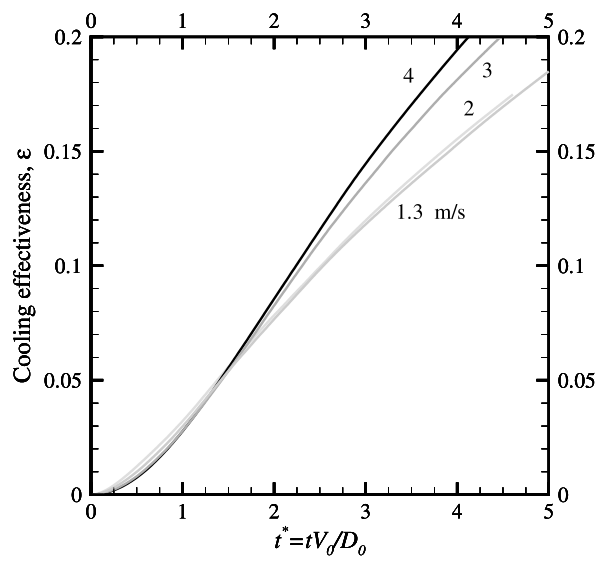
\includegraphics[width=0.5\linewidth]{Figures/2.Chapter/cooling.png}
\caption {Evolution of the calculated cooling effectiveness during the impact of a droplet on a surface initially at 120ºC}
\label{fig:cooling}
\source{M. Pasandideh-Fard, 2001 \cite{pasandideh2001cooling}}
\end{figure}

\par The heat transfer occurring during droplet spreading has particular complex characteristics as described in the literature (e.g. \cite{strotos2011non}). Figure \ref{fig:tempvar} illustrates approximately how the temperature of the surface evolves along the radius during droplet spreading. In the center of the droplet a bubble trapping effect creates a barrier for heat transfer, causing the temperature to have a slightly higher value. Also in the minimum thickness area the temperature is higher because the layer of liquid is thinner, removing less heat. In the contact edge, called rim, the liquid flowing from the lamella arrives and recirculates, so the temperature decreases again in this regime. The temperature raise at the end of the droplet, after the rim is naturally due to heat conduction from the heater within a region that is no longer wetted by the fluid.\\

\begin{figure}[h]
\centering
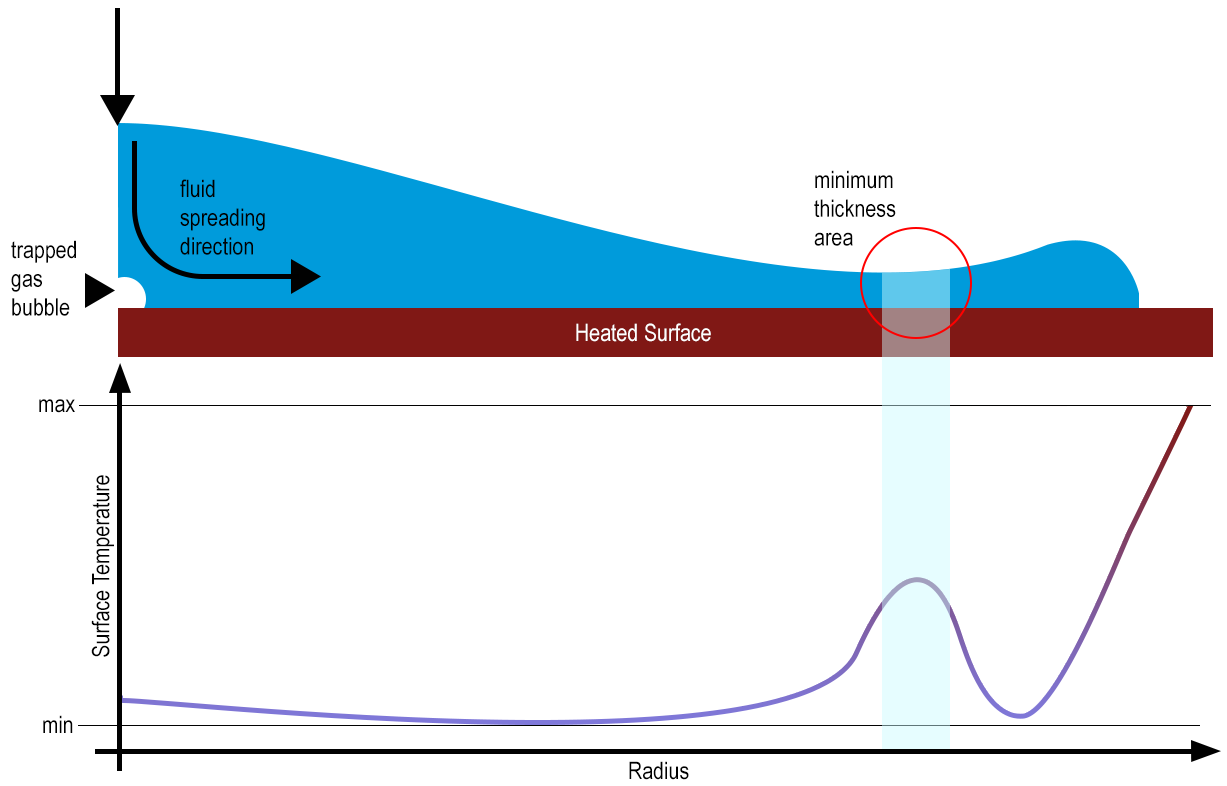
\includegraphics[width=1\linewidth]{Figures/2.Chapter/tempvar.png}
\caption {Scheme of the surface temperature variation along the droplet radius, during spreading}
\label{fig:tempvar}
\end{figure}



\cleardoublepage

\chapter{Experimental Setups}
\label{cap:setup}

%\textit{In this chapter the experimental setups used will be shown and explained in detail.}

% \section{Introduction}

% The experimental setups used in this work had two main themes: droplets on heated surfaces and pool boiling. In the Droplets Experiments a vertical and horizontal view were considered, but in the boiling experiments, because of the water opacity to IR radiation, only the vertical experiment was made.


\section{Introduction}

\par This Chapter describes the experimental setups used in the present work, together with the respective procedures. Two setups are used to obtain side views of the droplet (to understand its dynamics) and bottom view of the surface, to obtain temperature maps of the surface region cooled by the impact of the droplet.\\

\section{The Infrared (IR) Camera}
\label{sec:icam}
The IR Camera, an Onca-MWIR-InSb from Xenics, is the main device used in this dissertation provides "images" of the analyzed object's temperature field. Its 2D array of sensors reads the incident IR radiation. Its signal is then converted to temperature in the camera's software. The user will end up with a bi-dimensional field of temperatures with a +/- 0.5ºC precision. This camera can be seen in Figure \ref{fig:onca}.

\begin{figure}[h!]
\centering
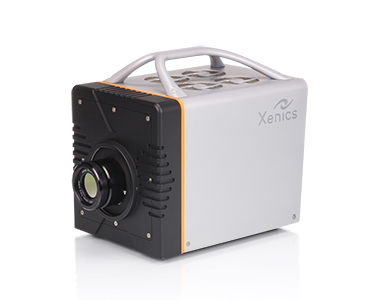
\includegraphics[width=0.6\linewidth]{Figures/2.Chapter/onca.png}
\caption{Xenics' Onca-MWIR-InSb}
\source{http://www.xenics.com/en/onca-mwir-insb}
\label{fig:onca}
\end{figure}

\subsection{Camera properties}

\par The relevant properties of the Onca-MWIR-InSb can be seen in Table \ref{tab:camprop}.

\begin{table}[h]
\centering
\caption{Camera Properties}
\label{tab:camprop}
\begin{tabular}{lclclc}
\toprule
\multicolumn{2}{c}{Camera Characteristics} & \multicolumn{2}{c}{Optical System} & \multicolumn{2}{c}{Image Characteristics} \\
\cmidrule[0.4pt](r{0.125em}){1-2}%
\cmidrule[0.4pt](r{0.125em}){3-4}%
\cmidrule[0.4pt](r{0.125em}){5-6}%
Sensor                 & InSb (MWIR)       & Focal lens          & 13 mm        & Video Rate         & 60Hz                 \\
Spectral Sensibility   & 3.5-5 $\mu m$     & Optics Material     & Germanium    & Max framerate      & 3000 fps             \\
Spatial Resolution     & $320 \times 256$ px &  -                  & -            & Min pixels (ROI)   & $15 \times 5$ px        \\
Thermal Sensibility    & \textless17mk     &   -                 &   -          & Exposition         & \textgreater 1 $\mu s$  \\ \bottomrule
\end{tabular}
\end{table}


\subsection{The Software}

\par This camera has its own specific software, Xeneth, which will be very important throughout this work. It's relevant to explain its functioning, which will be referenced various times in this dissertation. The correct use of the camera also depends on an appropriate configuration of several parameters on the software which therefor are worth to be explored with more detail.

\subsubsection{Selecting a Calibration Pack}

\par When the program is executed a menu will appear. In this menu it's possible to select not only the used camera (there is also an option to select a virtual camera, used to play previously recorded videos) but also to select a calibration pack as it is shown in Figure \ref{fig:consetup}.
\begin{figure}[h]
\centering
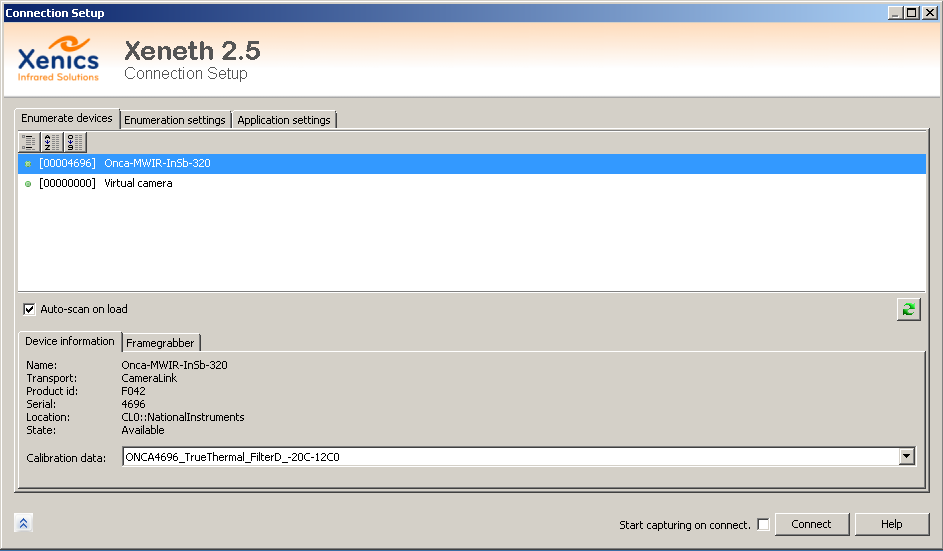
\includegraphics[width=0.7\linewidth]{Figures/3.Chapter/xeneth1.png}
\caption{Xeneth: Connection Setup Menu}
\label{fig:consetup}
\end{figure}
\par In the Calibration data drop menu are available several calibration packs. The main packs are:
\begin{itemize}
\item TRUE NUC: This pack is the one chosen if one wants to get data without temperature conversion. It presents results in Analogue to Digital Units (ADU) (received signal intensity) and it's adaptable to any integration time
\item TRUE THERMAL: This pack comes with a calibration made by the camera manufacturer, so the results are presented in Celsius. This is used if the user just needs a low thermal resolution measure or a qualitative result. It allows temperature measurements from -20 to 120ºC in any integration time (the integration time will be described in the following subsection).
\item User Calibration Packs: The user may want to create his own custom made pack adapted to his own temperature interval, to use in a more specific application.
\end{itemize}

\subsubsection{Main Window}
\label{software}
\par After choosing the appropriate calibration for the desired application and before starting the measurements, one should adjust several parameters in the main software window. The displayed panels are shown in Figure \ref{fig:xeneth2}. There is a panel for the Camera Image, where one can see the thermal image and select an area or dot to take its read value and other statistics; a User Interaction Panel, where one can change settings, view and set the selection properties, record and save videos and choose image filters; a panel that shows the plotted measured data. In the right side we can also see a colour bar. This bar is adjustable so that we can adapt the colour gradient to the desired temperature interval to better observe the phenomena. \\
\begin{figure}[h]
\centering
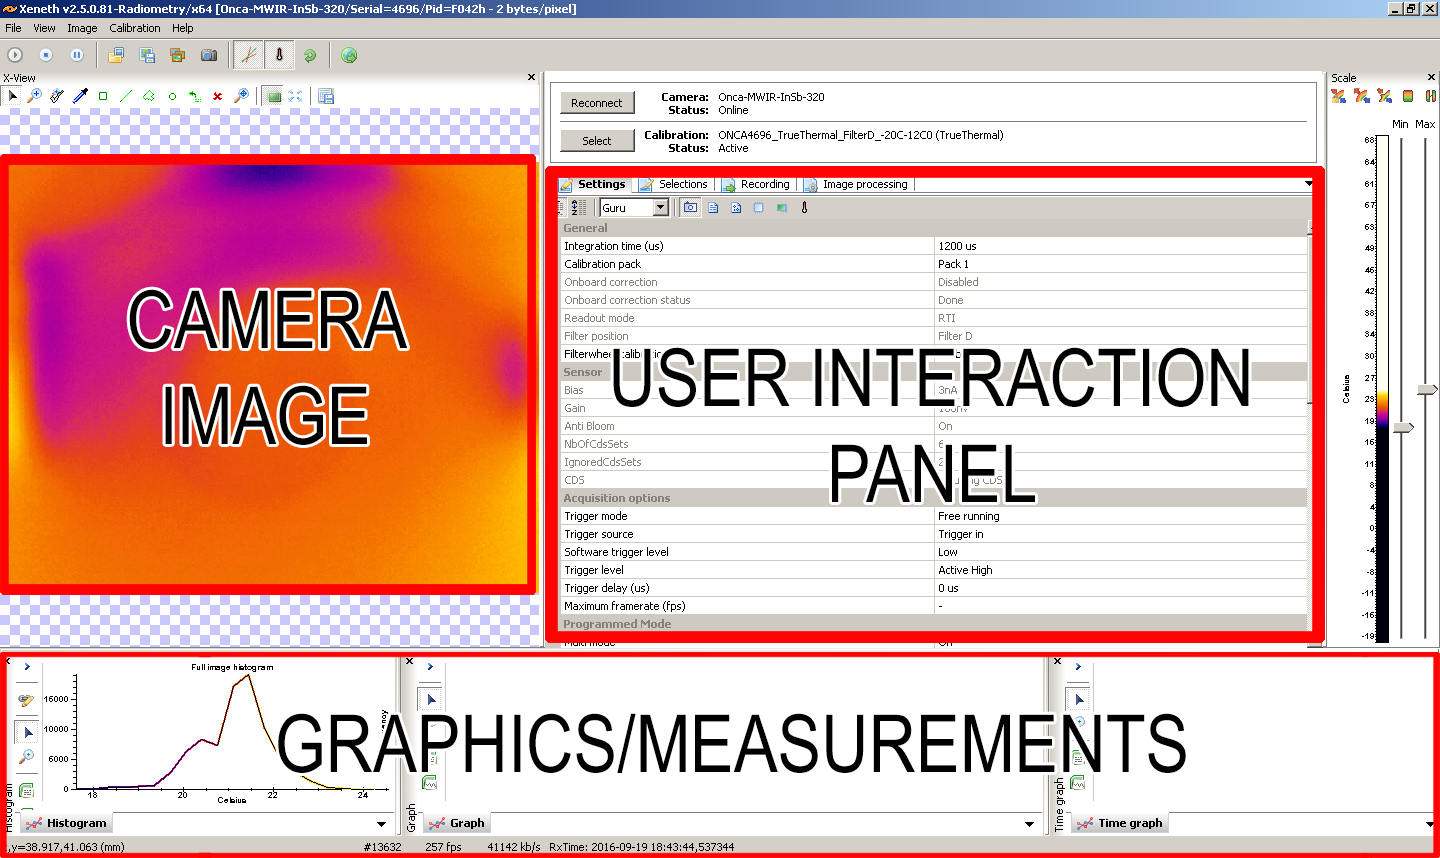
\includegraphics[width=0.7\linewidth]{Figures/3.Chapter/xeneth2.png}
\caption{Xeneth: Main Window Scheme}
\label{fig:xeneth2}
\end{figure}
\par Before starting there are some important settings to review to assure the best image possible. These parameters can be altered in the User Interaction Panel. The first and one of most important parameters is the integration time. The integration time can be easily explained as the equivalent to a common camera's exposure. If we increase the integration time we increase the sensitivity and reduce the noise. On the other side the image will saturate easier, which means that the temperature range highly decreases. So if a higher temperature range is needed, one should decrease the integration time until the desired range is obtained. Increasing the integration time will also decrease the acquisition rate (fps) which may not be relevant for static measurements, but the phenomena studied in this dissertation requires high temporal resolution because their characteristic time is of the order of milliseconds. The next important parameter to get is the Ambient Temperature and the Atmospheric Temperature, which can also be altered this in the User Interaction Panel. To determine the Ambient Temperature a highly reflective object is put in front of the camera and its temperature measured considering the body to be black. \\
\par The measurements can be made using the Selection Panel, shown in Figure \ref{fig:xeneth3}. In this panel it is possible to select a shape (a circle in the case presented) and gather the statistics about the temperature data, including the average temperature of the selected area both in space and time and also the standard deviation. This procedure is also used to select the area of interest. Finally the Zoom function is very important to restrict the measured area as much as it is possible to increase the acquisition rate of the camera. \\
\begin{figure}[h]
\centering
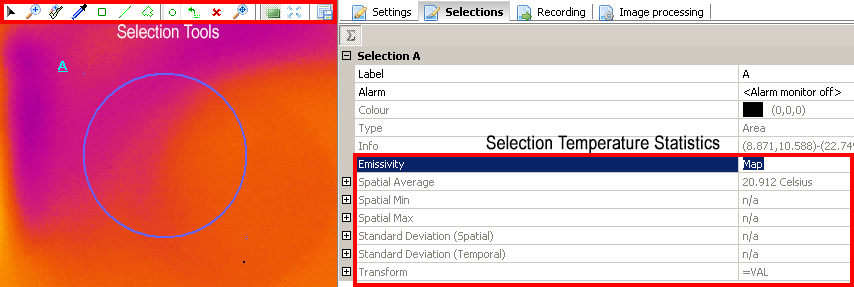
\includegraphics[width=0.7\linewidth]{Figures/3.Chapter/xeneth3.png}
\caption{Xeneth: Selection Panel}
\label{fig:xeneth3}
\end{figure}
\subsubsection{Offset Calibration}
\par The offset calibration is required to decrease the Narcissus effect, which is basically the reflection of the lens on itself, being an error source which must be eliminated. An example of this effect is illustrated in Figure \ref{fig:xeneth5} where a blackbody with constant temperature may happen to have temperature variations (Figure \ref{fig:xeneth5}.a).

\begin{figure}[h]
\centering
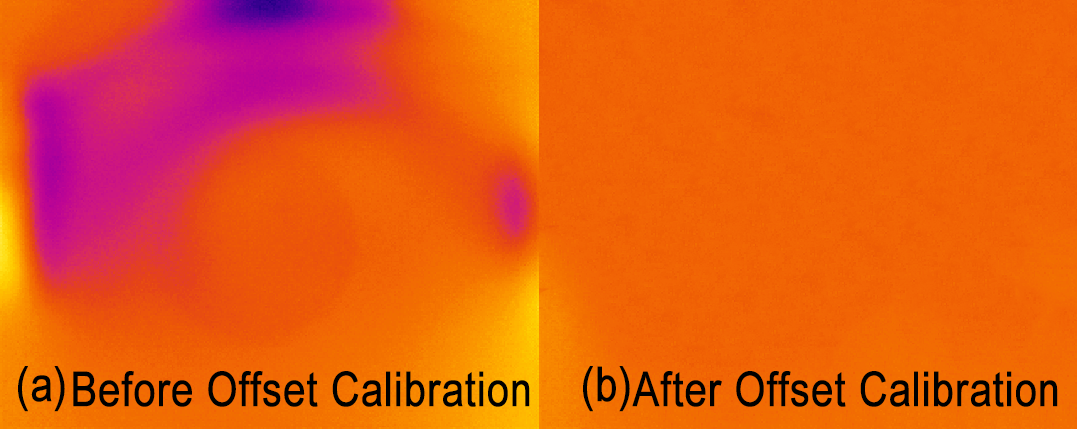
\includegraphics[width=0.7\linewidth]{Figures/3.Chapter/xeneth5.png}
\caption{Offset Calibration: Before and After}
\label{fig:xeneth5}
\end{figure}
\par A good way to eliminate this error is to use a software tool: the Offset Calibration. This can be found in the Calibration Wizard (a menu of calibration options for the camera) and has a simple function: it averages the temperature in space and time and sets every pixel to that temperature. This eliminates the camera's reflection and also part of the noise and bad pixels. A disadvantage of this method is that it may create lesser periodic noise, which can be a problem to the measurements. The code behind this function is unknown, so the noise source could not be detected and could only be attenuated later in the post-processing stage. The result of the Offset Calibration can be seen in Figure \ref{fig:xeneth5}.b. \\

\section{Experimental set up to obtain profile views of the droplet}

\par To create a heater, cartridge resistance heaters were put under an aluminum plate, radiating to its surface. The experiment was made for water droplets impacts on a hydrophilic silicon wafer surface \\

\par In the interface of the silicon wafer and the aluminum plate a thermal paste was used to improve heat transfer. On top of the silicon wafer there is a thermocouple that monitors the surface temperature. This setup can be seen in detail in Figure \ref{fig:horizontal2}. The thermocouple value is used by a PID controller to control the heat released by the cartridge heater.\\

\begin{figure}[h]
\centering
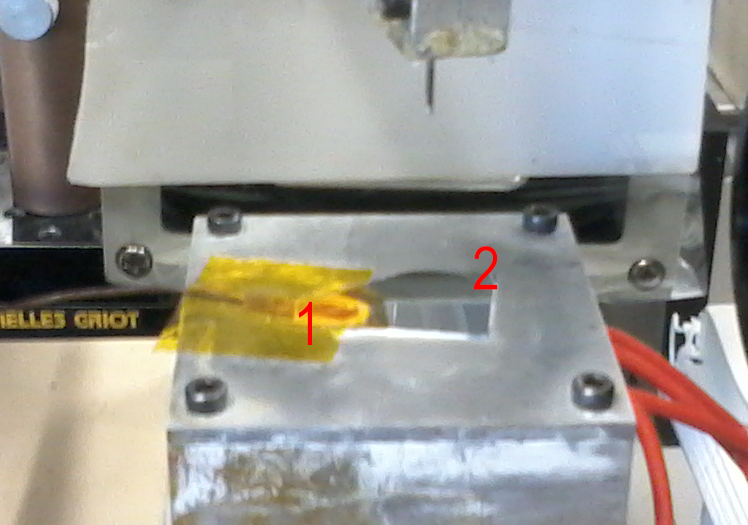
\includegraphics[width=0.5\linewidth]{Figures/3.Chapter/horizontal2.png}
\caption{Silicon Wafer setup: (1) Thermocouple, (2) Silicon Wafer}
\label{fig:horizontal2}
\end{figure}

\par An Harvard Apparatus controls a syringe's water discharge, that then falls from the needle to the wafer. This forms a droplet with 2.6 to 3 mm diameter spherical droplet. This experiment is recorded by 2 cameras: IR camera and high-speed camera. In order for the high-speed camera to work, a high intensity lamp is also needed. The described setting can be seen in Figure \ref{fig:horizontal}. This setting was used to gather qualitative results only. Good quantitative results are impossible due to the implications of droplet geometry in thermography. The images taken by the high speed camera were recorded at 2200 fps. The calibration factor used was 26 px/mm. The calibration factor for the IR camera was 6 px/mm.

\begin{figure}[h]
\centering
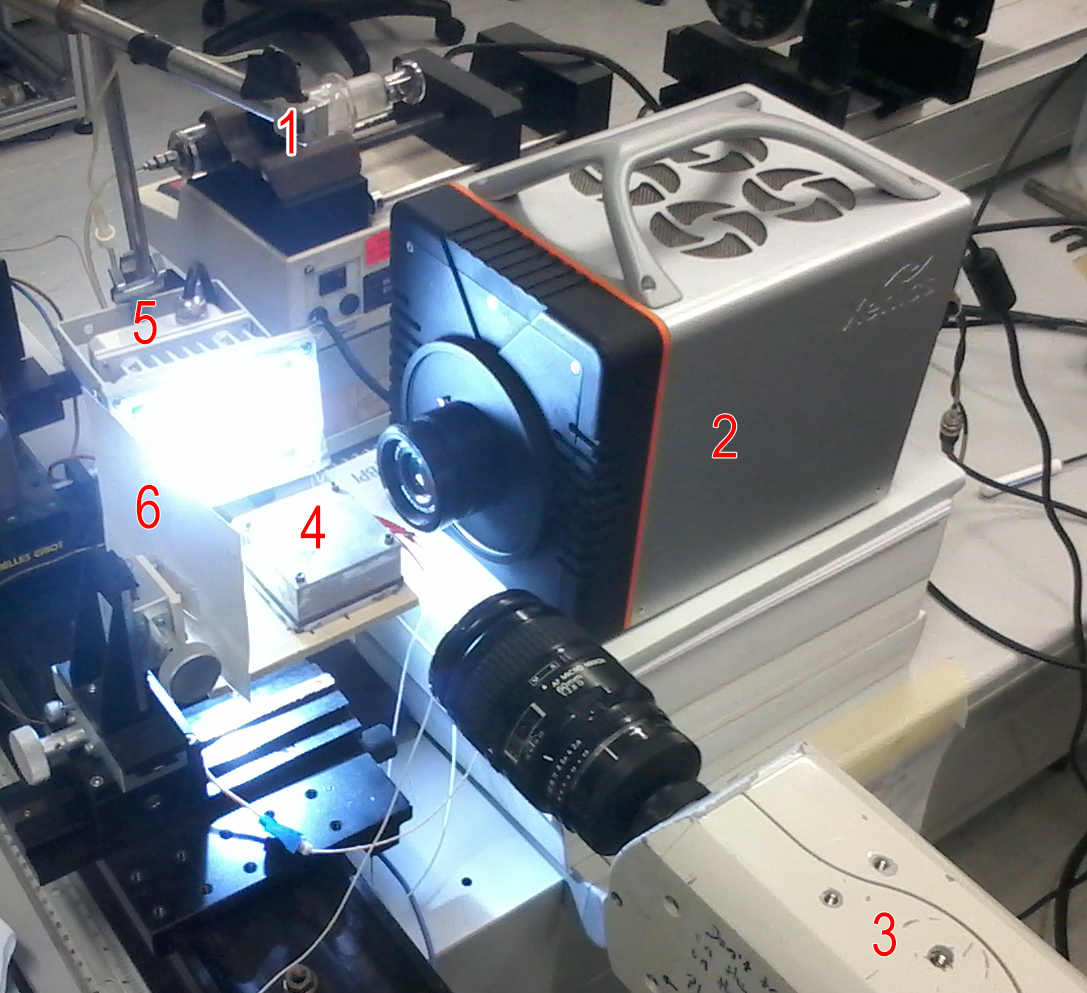
\includegraphics[width=0.65\linewidth]{Figures/3.Chapter/horizontal.png}
\caption{Horizontal setup: (1) Needle, (2) IR Camera, (3) HS Camera, (4) Heated Surface, (5) Lamp, (6) Black Background}
\label{fig:horizontal}
\end{figure}

\subsection{Procedure}
\label{sec:procedure}
\begin{itemize}
\item Adjust IR Camera's settings on the software.
\item Perform an offset calibration (described in Section \ref{sec:icam}).
\item Adjust PID controller to the desired temperature and water flow in the Harvard Apparatus.
\item Set the cameras recording.
\item Let a droplet fall on the wafer.
\item Clean the wafer with acetone and distilled water before proceeding to a new test.
\end{itemize}

\section{Bottom View of the metal foil}

\par In this setup, the IR Camera is placed underneath the surface on which the droplet impacts. The droplet impacts on a 20 $\mu m$ thick stainless steel foil. This was done similarly to \cite{sielaff2014experimental}, as the objective was to read the interface temperatures. Due to of the small thickness of the foil, the temperature of the interface is very similar to the read temperature in the bottom of the foil. The HS camera was placed horizontally to the foil to observe the impact. A lamp was placed in the opposite side. The setup scheme can be seen in Figure \ref{fig:setup}.\\

\begin{table}[h]
\centering
\caption{Thermophysical Properties of the Studied Liquids}
\label{tab:props}
\begin{tabular}{lcc}
\toprule
\multicolumn{1}{c}{Characteristics} & \multicolumn{1}{c}{Water} & \multicolumn{1}{c}{Ethanol} \\
\cmidrule[0.4pt](r{0.125em}){1-3}%
Saturation Temperature ($T_{sat}[ºC]$)       & 100                 & 78.3         \\
Density ($\rho[kg/m^3]$)                   & 1000                & 757          \\
Kinematic Viscosity ($\mu[10^{-3}Ns/m^2]$) & 1.05                & 1.19         \\
Surface Tension ($\sigma[10^{-3}N/m]$)     & 72.88               & 22.8         \\ \bottomrule
\end{tabular}
\end{table}

\begin{figure}[h]
\centering
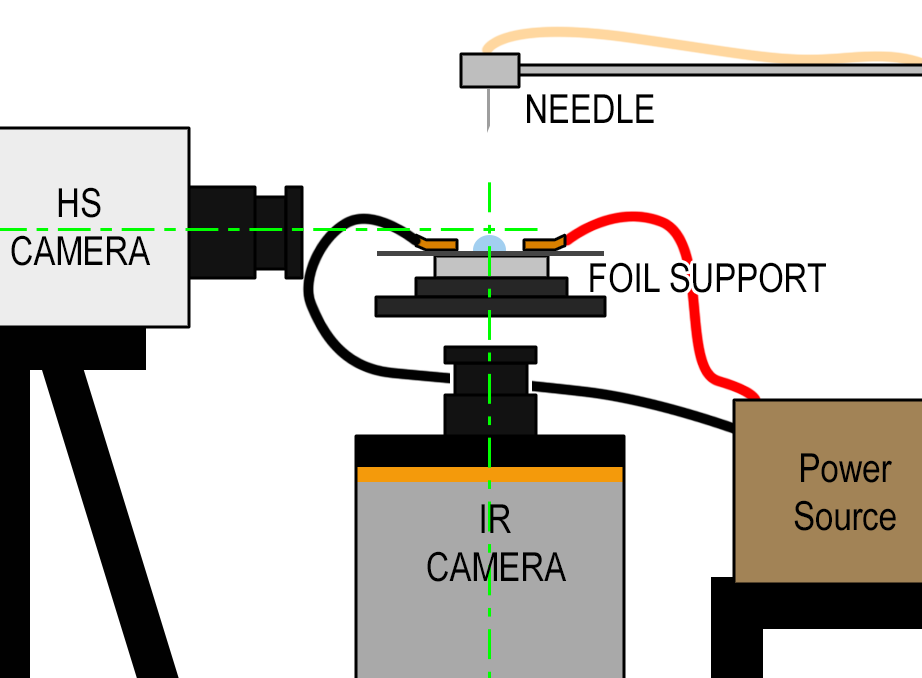
\includegraphics[width=0.55\linewidth]{Figures/3.Chapter/setup.png}
\caption{Bottom Setup Scheme}
\label{fig:setup}
\end{figure}

\par The experiments performed using this setup were made using hydrophilic (using distilled water and ethanol) and super-hydrophobic (using just water) surfaces. A preliminary experiment with water and an hydrophilic surface was made, using the software calibration. From the first, raw results were taken for posterior calibration and processing. The calibrations and their differences are explained in Chapter \ref{cap:setup}. Table \ref{tab:props} summarizes the main physical properties of the working fluids \cite{tfc}.\\

\par The foil is fed by an electric current, so it can heat up to the desired temperature. This is done by to electrical contacts, wired to a power source. The foil has to be placed on top of a bad heat conductor to minimize heat losses. A heat glass was chosen for the purpose. The foil must be stretched so that possible wrinkles don't affect the droplet motion. A detail of the setup, on the foil support can be seen in Figure \ref{fig:suporte}. In this figure two supports are shown. The second was made after the calibration. \\

\par To prepare the super-hydrophobic surfaces, the surfaces needed to be cleaned with an ultra-sound bath and coated with \textit{Glaco}\textregistered \cite{kato2011durable}. This coating took several layers to ensure effective coating that can endure high temperature and droplet impacts. \\

\begin{figure}[h]
\centering
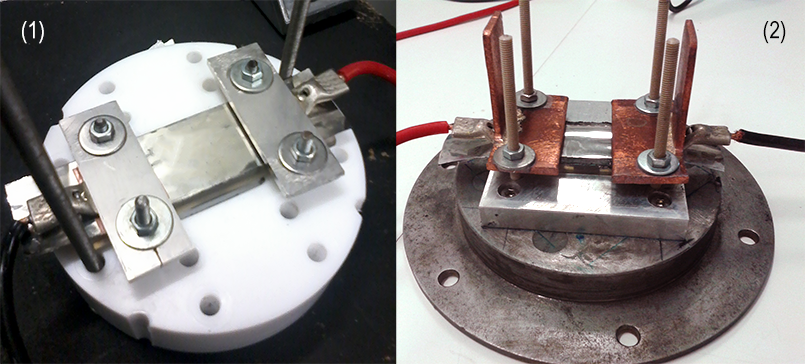
\includegraphics[width=0.9\linewidth]{Figures/3.Chapter/suporte.png}
\caption{Stainless Steel Support: (1) Before calibration setup, (2) After calibration setup}
\label{fig:suporte}
\end{figure}

\par This setup also was the Harvard Apparatus and the needle to generate the droplet. A metal structure holds the support, needle and the camera. The complete setup can be seen in Figure \ref{fig:setup2}. Although one have a different calibration, the procedure is similar to the previously described in \ref{sec:procedure}. The big difference is that the foil temperature is controlled with the power source and not with the PID. To adjust the current correctly one needs to read the temperature on the IR Camera's software. In the case that raw images are needed, an additional step should be to convert the desired temperatures in ADU. Only this procedure allows knowing if the foil is at the desired temperature.

\begin{figure}[h]
\centering
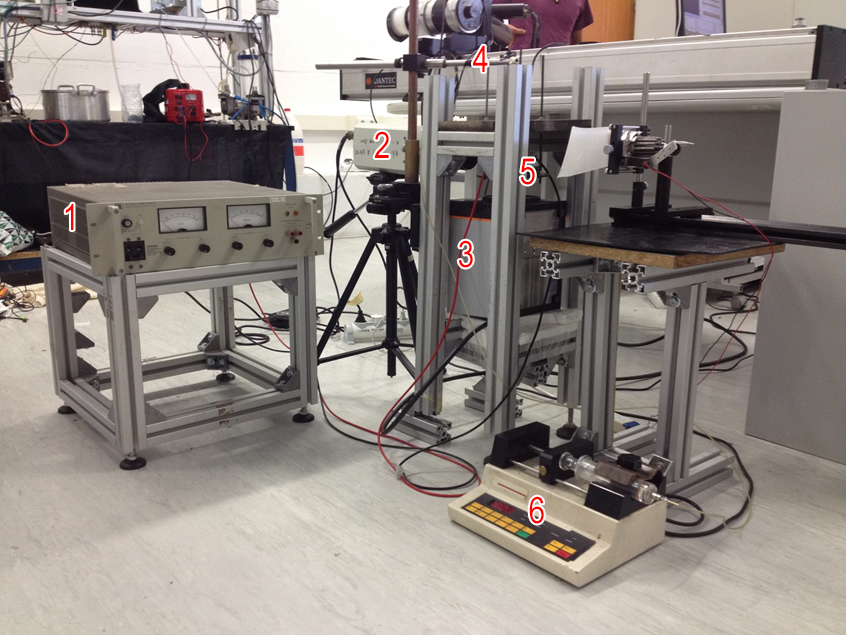
\includegraphics[width=0.9\linewidth]{Figures/3.Chapter/setup2.png}
\caption{Bottom Setup: (1) Power Source, (2) HS Camera, (3) IR Camera, (4) Needle, (5) Foil Support, (6) Harvard Apparatus}
\label{fig:setup2}
\end{figure}

\section{Surface preparation and Characterization}
\par The stainless steel foils (coated and uncoated) were characterized in terms of surface topography and wettability. Surface topography was measured a profile meter (Dektak 3 - Veeco) with a vertical resolution of 20 nm. The foil was found to be smooth within this resolution. The wettability was characterized measuring the contact angle with an optical profile meter (THETA from Attention) using the droplet method, as described for instance in Moita \textit{et. al.} (2016) \cite{moita2016dynamics}. The contact angle values are taken as an average of 5 measurements performed at different regimes of the surfaces. The contact angle is $\theta = 87.05º$ for the hydrophilic surface and $\theta = 162.47º$ for the super-hydrophobic surface.\\
\par Hysterisis, evaluated also as in Moita \textit{et. al.} (2016) \cite{moita2016dynamics} was found to be lower than 10º for the surface with the highest contact angle (coated with \textit{Glaco}\textregistered) thus confirming its super-hydrophobic nature.
%%
\section{Experimental set up to obtain profile views of the droplet}

\par To create a heater, cartridge resistance heaters were put under an aluminum plate, radiating to its surface. The experiment was made for water droplets impacts on a hydrophilic silicon wafer surface \\

\par In the interface of the silicon wafer and the aluminum plate a thermal paste was used to improve heat transfer. On top of the silicon wafer there is a thermocouple that monitors the surface temperature. This setup can be seen in detail in Figure \ref{fig:horizontal2}. The thermocouple value is used by a PID controller to control the heat released by the cartridge heater.\\

\begin{figure}[h]
\centering
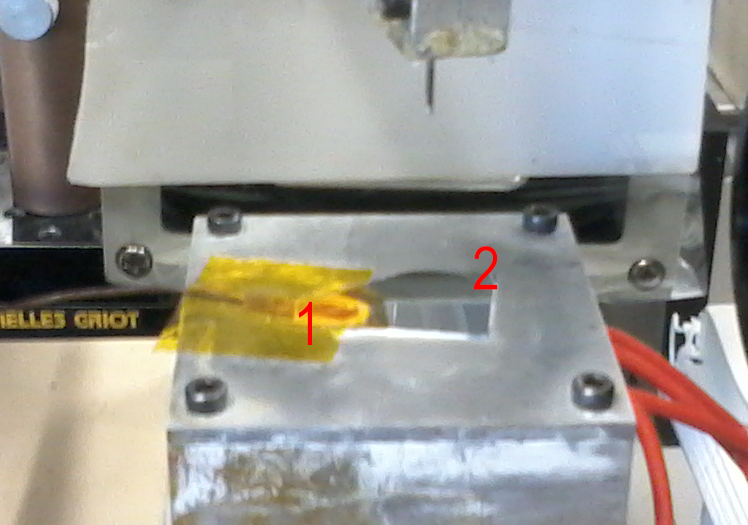
\includegraphics[width=0.5\linewidth]{Figures/3.Chapter/horizontal2.png}
\caption{Silicon Wafer setup: (1) Thermocouple, (2) Silicon Wafer}
\label{fig:horizontal2}
\end{figure}

\par An Harvard Apparatus controls a syringe's water discharge, that then falls from the needle to the wafer. This forms a droplet with 2.6 to 3 mm diameter spherical droplet. This experiment is recorded by 2 cameras: IR camera and high-speed camera. In order for the high-speed camera to work, a high intensity lamp is also needed. The described setting can be seen in Figure \ref{fig:horizontal}. This setting was used to gather qualitative results only. Good quantitative results are impossible due to the implications of droplet geometry in thermography. The images taken by the high speed camera were recorded at 2200 fps. The calibration factor used was 26 px/mm. The calibration factor for the IR camera was 6 px/mm.

\begin{figure}[h]
\centering
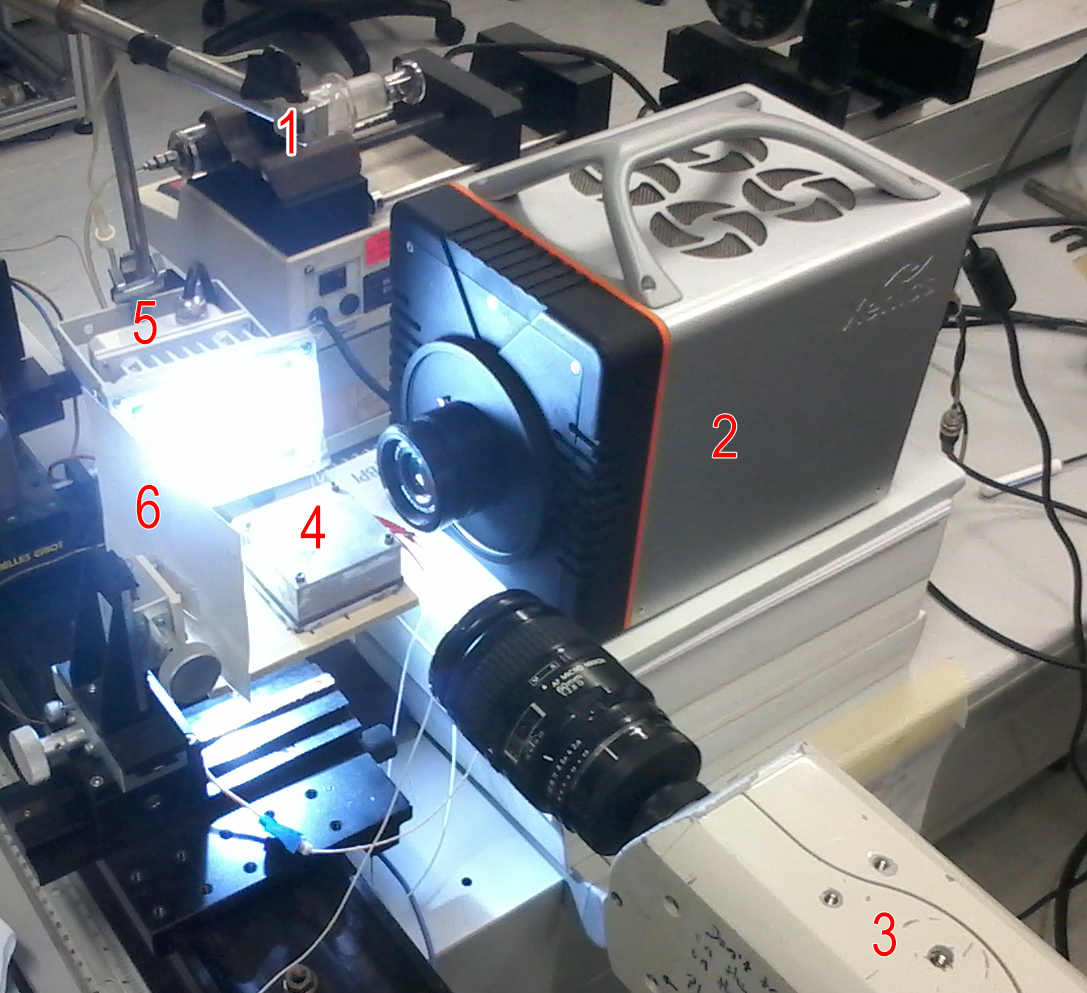
\includegraphics[width=0.65\linewidth]{Figures/3.Chapter/horizontal.png}
\caption{Horizontal setup: (1) Needle, (2) IR Camera, (3) HS Camera, (4) Heated Surface, (5) Lamp, (6) Black Background}
\label{fig:horizontal}
\end{figure}

\subsection{Procedure}
\label{sec:procedure}
\begin{itemize}
\item Adjust IR Camera's settings on the software.
\item Perform an offset calibration (described in Section \ref{sec:icam}).
\item Adjust PID controller to the desired temperature and water flow in the Harvard Apparatus.
\item Set the cameras recording.
\item Let a droplet fall on the wafer.
\item Clean the wafer with acetone and distilled water before proceeding to a new test.
\end{itemize}

\section{Bottom View of the metal foil}

\par In this setup, the IR Camera is placed underneath the surface on which the droplet impacts. The droplet impacts on a 20 $\mu m$ thick stainless steel foil. This was done similarly to \cite{sielaff2014experimental}, as the objective was to read the interface temperatures. Due to of the small thickness of the foil, the temperature of the interface is very similar to the read temperature in the bottom of the foil. The HS camera was placed horizontally to the foil to observe the impact. A lamp was placed in the opposite side. The setup scheme can be seen in Figure \ref{fig:setup}.\\

\begin{table}[h]
\centering
\caption{Thermophysical Properties of the Studied Liquids}
\label{tab:props}
\begin{tabular}{lcc}
\toprule
\multicolumn{1}{c}{Characteristics} & \multicolumn{1}{c}{Water} & \multicolumn{1}{c}{Ethanol} \\
\cmidrule[0.4pt](r{0.125em}){1-3}%
Saturation Temperature ($T_{sat}[ºC]$)       & 100                 & 78.3         \\
Density ($\rho[kg/m^3]$)                   & 1000                & 757          \\
Kinematic Viscosity ($\mu[10^{-3}Ns/m^2]$) & 1.05                & 1.19         \\
Surface Tension ($\sigma[10^{-3}N/m]$)     & 72.88               & 22.8         \\ \bottomrule
\end{tabular}
\end{table}

\begin{figure}[h]
\centering
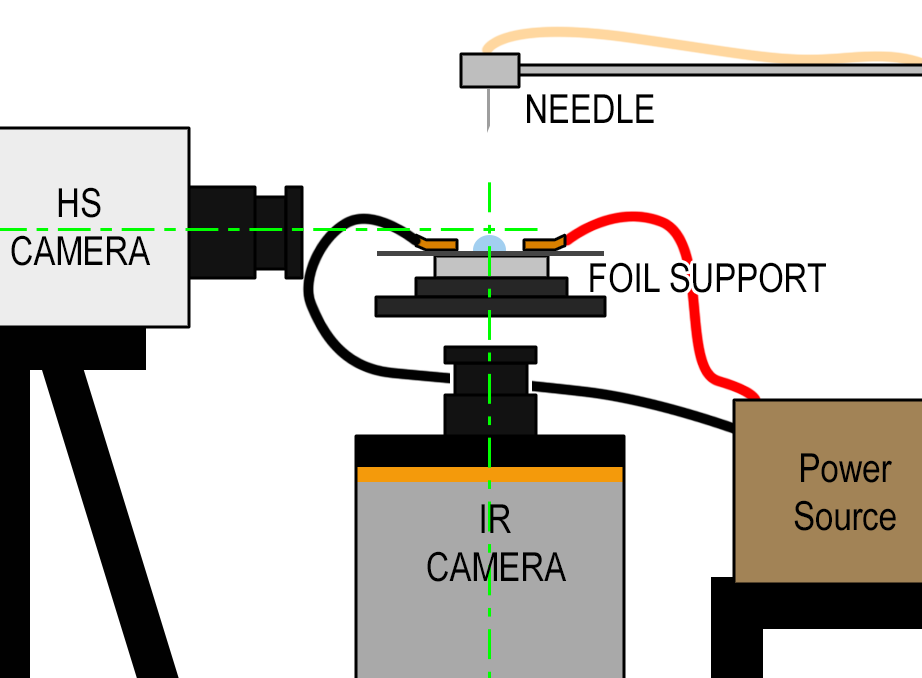
\includegraphics[width=0.55\linewidth]{Figures/3.Chapter/setup.png}
\caption{Bottom Setup Scheme}
\label{fig:setup}
\end{figure}

\par The experiments performed using this setup were made using hydrophilic (using distilled water and ethanol) and super-hydrophobic (using just water) surfaces. A preliminary experiment with water and an hydrophilic surface was made, using the software calibration. From the first, raw results were taken for posterior calibration and processing. The calibrations and their differences are explained in Chapter \ref{cap:setup}. Table \ref{tab:props} summarizes the main physical properties of the working fluids \cite{tfc}.\\

\par The foil is fed by an electric current, so it can heat up to the desired temperature. This is done by to electrical contacts, wired to a power source. The foil has to be placed on top of a bad heat conductor to minimize heat losses. A heat glass was chosen for the purpose. The foil must be stretched so that possible wrinkles don't affect the droplet motion. A detail of the setup, on the foil support can be seen in Figure \ref{fig:suporte}. In this figure two supports are shown. The second was made after the calibration. \\

\par To prepare the super-hydrophobic surfaces, the surfaces needed to be cleaned with an ultra-sound bath and coated with \textit{Glaco}\textregistered \cite{kato2011durable}. This coating took several layers to ensure effective coating that can endure high temperature and droplet impacts. \\

\begin{figure}[h]
\centering
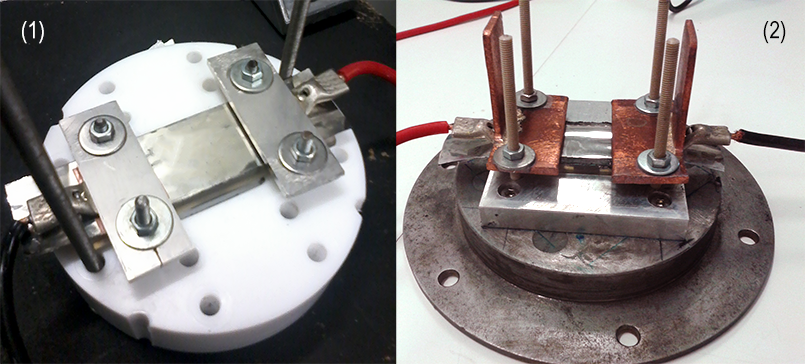
\includegraphics[width=0.9\linewidth]{Figures/3.Chapter/suporte.png}
\caption{Stainless Steel Support: (1) Before calibration setup, (2) After calibration setup}
\label{fig:suporte}
\end{figure}

\par This setup also was the Harvard Apparatus and the needle to generate the droplet. A metal structure holds the support, needle and the camera. The complete setup can be seen in Figure \ref{fig:setup2}. Although one have a different calibration, the procedure is similar to the previously described in \ref{sec:procedure}. The big difference is that the foil temperature is controlled with the power source and not with the PID. To adjust the current correctly one needs to read the temperature on the IR Camera's software. In the case that raw images are needed, an additional step should be to convert the desired temperatures in ADU. Only this procedure allows knowing if the foil is at the desired temperature.

\begin{figure}[h]
\centering
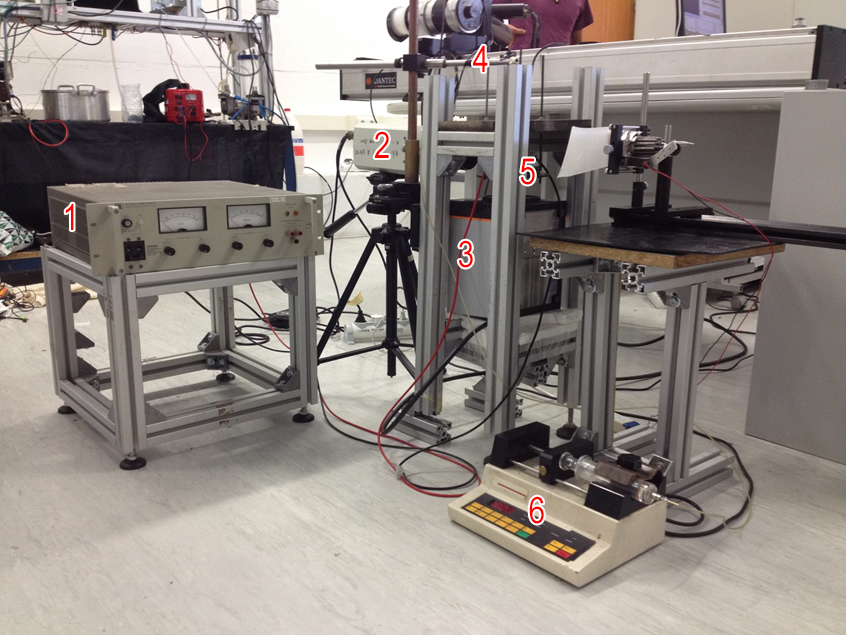
\includegraphics[width=0.9\linewidth]{Figures/3.Chapter/setup2.png}
\caption{Bottom Setup: (1) Power Source, (2) HS Camera, (3) IR Camera, (4) Needle, (5) Foil Support, (6) Harvard Apparatus}
\label{fig:setup2}
\end{figure}

\section{Surface preparation and Characterization}
\par The stainless steel foils (coated and uncoated) were characterized in terms of surface topography and wettability. Surface topography was measured a profile meter (Dektak 3 - Veeco) with a vertical resolution of 20 nm. The foil was found to be smooth within this resolution. The wettability was characterized measuring the contact angle with an optical profile meter (THETA from Attention) using the droplet method, as described for instance in Moita \textit{et. al.} (2016) \cite{moita2016dynamics}. The contact angle values are taken as an average of 5 measurements performed at different regimes of the surfaces. The contact angle is $\theta = 87.05º$ for the hydrophilic surface and $\theta = 162.47º$ for the super-hydrophobic surface.\\
\par Hysterisis, evaluated also as in Moita \textit{et. al.} (2016) \cite{moita2016dynamics} was found to be lower than 10º for the surface with the highest contact angle (coated with \textit{Glaco}\textregistered) thus confirming its super-hydrophobic nature.
\cleardoublepage
\chapter{Calibration and Data Processing Methods}
\label{cap:setup}

%\textit{In this chapter the IR Camera calibration will be discussed. The calibration is a big part of this dissertation, and the work revolving the calibration will be presented here.}
%\section{Introduction}
%\par The importance of quality calibration for this work is mainly justified by skepticism towards the camera's factory calibration and the quality of the used software. Because the camera's software presents big constraints and brings large sources of mistakes with unknown origins, the best way to process the results is to obtain the RAW data and treat it resorting to a special made Matlab code and a blackbody calibration. \\
\section{Blackbody Calibration Sources}
\par Black Body Calibration sources are recommended by the camera manual to calibrate the camera correctly. They are simply blackbodies with controllable temperature. The temperature controlled blackbody is to be filmed by the IR Camera and the camera's raw data (signal intensity received by the sensors) extracted. With a known temperature and high emissivity it is easy to correlate the signal intensity with the correspondent temperature. Establishing this relation can be done directly in the software but for the aforementioned reasons this was the procedure established and developed in this work.\\

\par The Blackbody Calibration Source is the name given to these devices, that are commercialized to calibrate infrared sensors. Given the high costs of these devices (over 7000 euros) a simple but functional Blackbody Calibration Source was projected and assembled in the present work.\\

\par There are several types of blackbody calibration sources, which are included in these main categories \cite{blackbody}: 
\begin{itemize}
\item Fixed-Point Blackbody Radiators: used at really high temperatures (>1000ºC), these are characterized by having a metal (eg. Au, Ag or Cu) at freezing point and a graphite made cavity (high emissivity). The quality of the measure is defined by the quality of the graphite, metal ingot and shape of the cavity.
\item Heat Pipe Cavities: used for applications with temperatures from -60ºC to 1000ºC, depending on the working fluid, these are characterized by having the best precision and being the most sophisticated devices. The cavity is surrounded by a multistate heated fluid at a controlled pressure. This cavity has special geometric properties to enhance the emissivity of the body. They are usually used in high precision applications for instance in meteorology institutes.
\item Pratical Cavities: used in more pratical applications, they are used for a range of temperatures between -45ºC and 450ºC. Unlike the Heat Pipe, the working fluid rarely changes its physical state (eg. one could only go up until 100ºC with water). Pratical cavities are easy to build and are often used for tests by radiation thermometers manufacturers. Similarly to the Heat Pipe Cavities also rely on specific geometric conditions to enhance the cavity's emissivity.
\item Flat Plate: these devices are used as an alternative to the pratical cavities because they do not require small cavities. As counterpart of in these devices, the heated plate must have a high emissivity, usually obtained using a high emissivity paint, so they may lead o large uncertainties. This method is usually used for large applications which do not require very accurate measurements.
\item Others: Cryogenic/Vaccum Blackbodies are used for extreme values of temperature such as negative temperatures ( as low as -100ºC) and Furnaces used in this case as a Flat plate for temperatures above 1000ºC.
\end{itemize}

\par For this work, the Pratical Cavity Radiator is the best choice, not only because it's often used for similar applications, within the same temperature range, but also because it is the simplest solution to build. The final design of the chamber was based on the scheme presented in Hartmann's work \cite{blackbody}, and it's illustrated in Figure \ref{fig:bbs}. The cavity shape is based on the design proposed in Figure \ref{fig:blkbody}. Since the camera had to be calibrated to work between 0 and 130ºC, the working fluid selected here was oil, with high saturation temperatures (300ºC at atmospheric temperature). \\

\begin{figure}
\centering
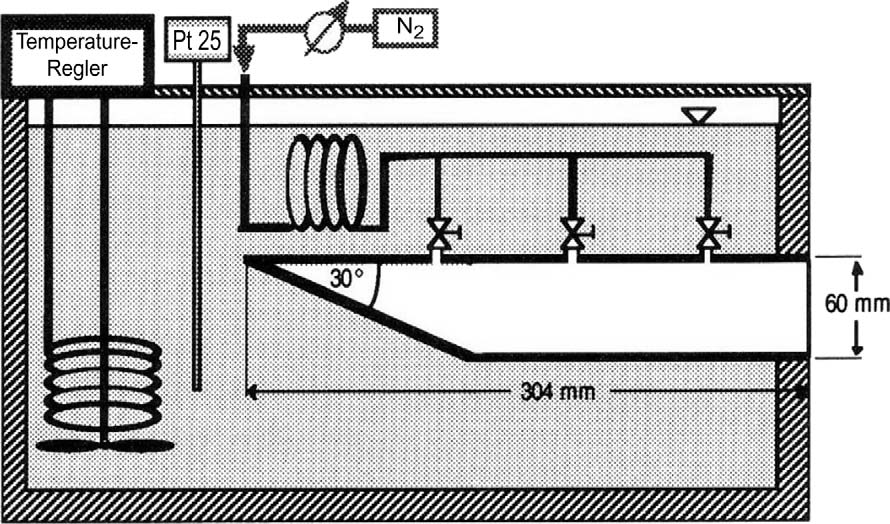
\includegraphics[width=0.6\linewidth]{Figures/4.Chapter/praticalcavity.png}
\caption{Pratical Cavity Blackbody Source scheme}
\source{Chapter 3.2 from \cite{blackbody}}
\label{fig:bbs}
\end{figure}


\par The effect of the cavity shape show in Figure \ref{fig:blkbody} is used in many cavity based Blackbody Radiator Devices and is used to enhance the emissivity, by trapping the light, thus reducing the light reflected from the outside. This effect is enhanced by an angle of 30º as referenced in the literature \cite{blackbody}. A working scheme of the final design of the created device, with a mixture of these 2 concepts is presented in Figure \ref{fig:box}. \\

\begin{figure}[h]
\centering
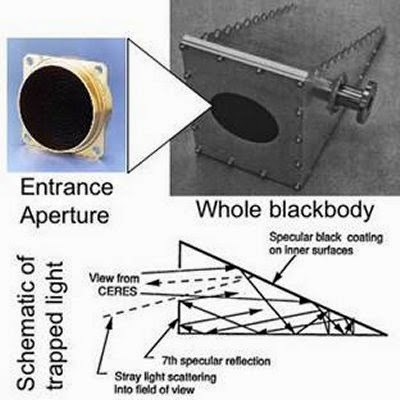
\includegraphics[width=0.6\linewidth]{Figures/4.Chapter/blackbody3.jpg}
\caption{Cavity and light trapping effect scheme}
\source{NASA}
\label{fig:blkbody}
\end{figure}

\begin{figure}[h]
\centering
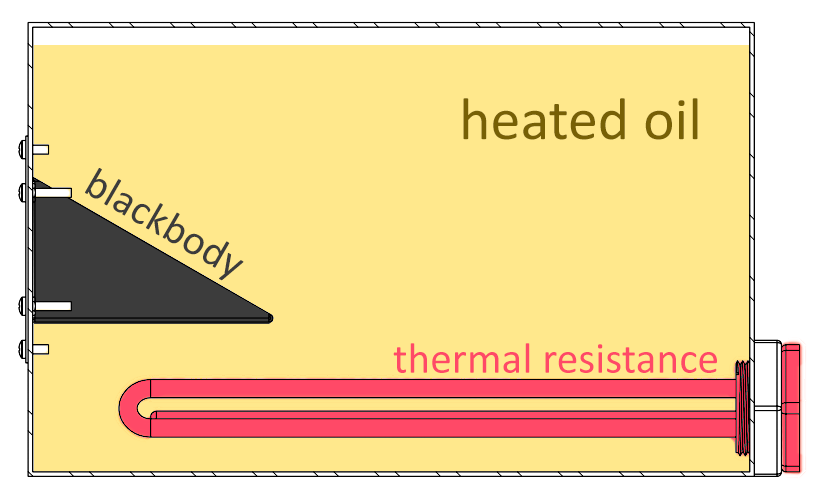
\includegraphics[width=0.6\linewidth]{Figures/4.Chapter/caixa.png}
\caption{Final design scheme for the Blackbody Calibration Source}
\label{fig:box}
\end{figure}

\subsection{Design details}
\par The final design render, made in SolidWorks, is depicted in Figure \ref{fig:render}. One may notice, both from the render and the scheme, that the box is too long compared to the blackbody. The reason for this is that the whole device had to be made to fit the thermal resistances which were commercially available. This resistance is presented in Figure \ref{fig:res}. The working fluid must have good conductive properties, so the type of oil used was car oil, which is stable under heating conditions. \\

\begin{figure}[h]
\centering
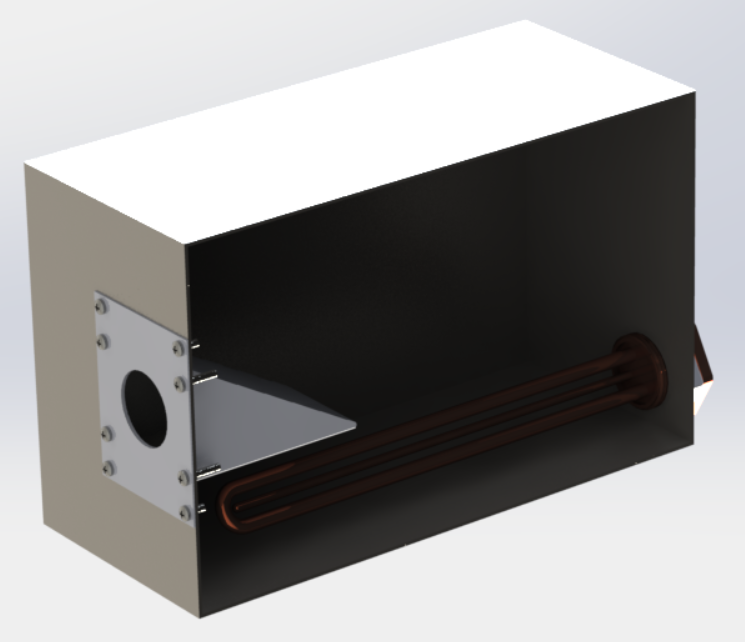
\includegraphics[width=0.8\linewidth]{Figures/4.Chapter/caixa_render.PNG}
\caption{SolidWorks render of a cut device view}
\label{fig:render}
\end{figure}

\par In both the scheme and render, the sensors, peripherals of the device and its insulation are omitted. Five type K thermocouples were used: 2 submerse thermocouples by each side of the blackbody to check if there were high temperature variations in different regions of the device; 3 surface thermocouples to monitor when the temperature stabilizes in the face of the device that is recorded by the IR camera (for the calibration procedure), and to provide enough temperature measurements from which one could take a good average of the real cavity temperature. The positioning of the thermocouples is schematically depicted in Figure \ref{fig:tpar}. \\

\begin{figure}[h]
\centering
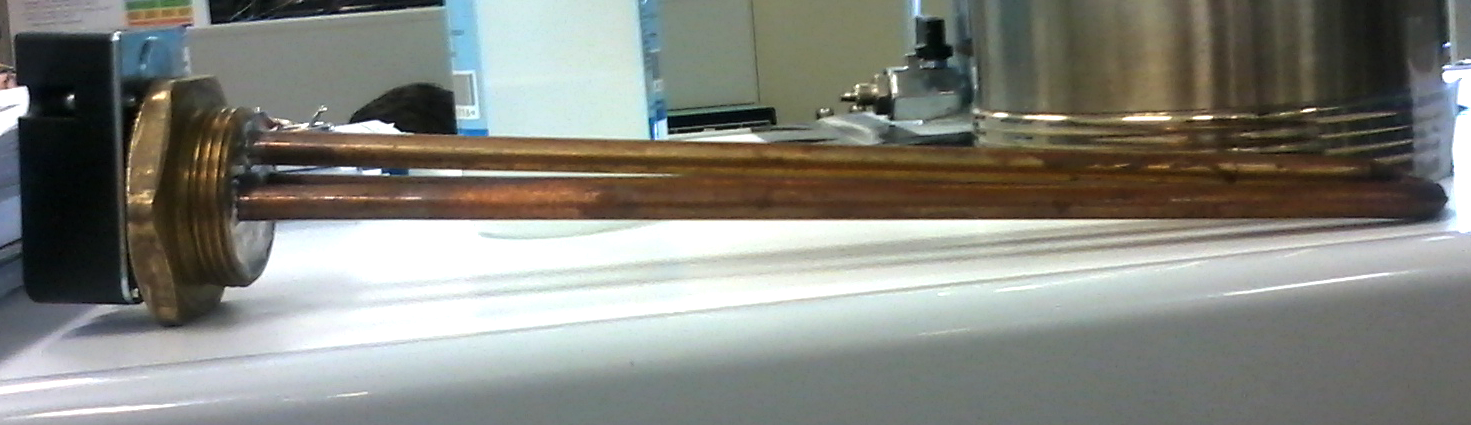
\includegraphics[width=0.9\linewidth]{Figures/4.Chapter/resistencia.png}
\caption{Thermal Resistance used}
\label{fig:res}
\end{figure}

\begin{figure}[h]
\centering
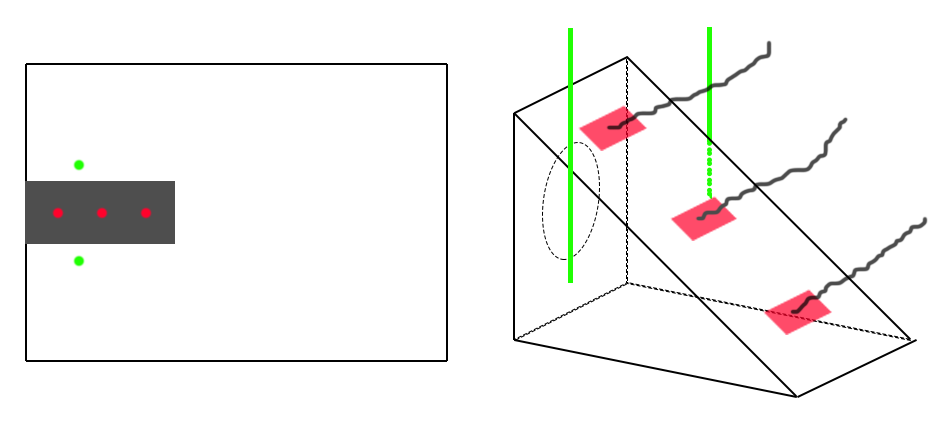
\includegraphics[width=0.9\linewidth]{Figures/4.Chapter/termopares.png}
\caption{Thermocouple placement scheme}
\label{fig:tpar}
\end{figure}

\par A KS 20-1 PID controller, that controls the resistance based on the temperature monitored by the middle surface thermocouple and a DT9828 Data Acquisition Board from Data Translation to connect the thermocouples to the computer were the data is processed.\\

\par Finally, the insulation consists of a 5mm PENA30FR adhesive, that is composed by sponge with aluminum coating. This material can be seen in Figure \ref{fig:isola}. The insulation is used all around the device and the only hole in it is the opening for the blackbody. \\

\begin{figure}[h]
\centering
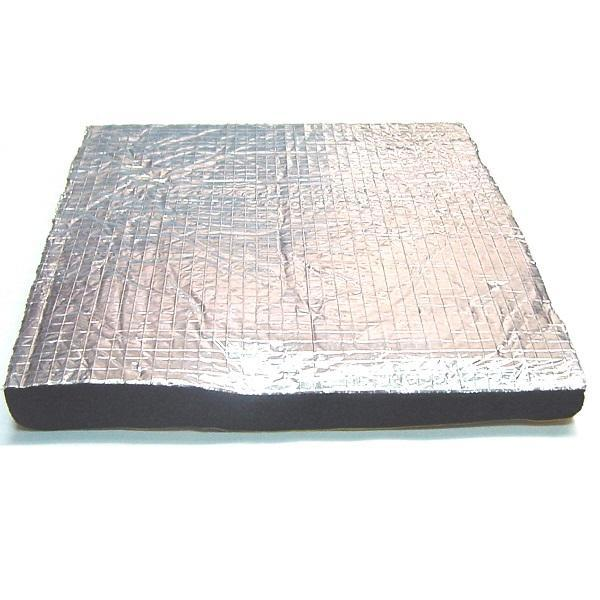
\includegraphics[width=0.5\linewidth]{Figures/4.Chapter/insulation.jpg}
\caption{PENA30FR Adhesive Insulation}
\label{fig:isola}
\end{figure}

\subsection{Building Process}

\par The building process of this device can be divided in 4 parts:

\begin{itemize}
\item The box: made in stainless steel, this box had to be ordered from a company specialized in metal work. The size of this box is 200x200x320 mm, with 2mm thickness. It already has 2 orifices to assemble the resistance and the blackbody. Thermal insulation was made to fit the box measures. The box is insulated only when both the blackbody and resistance are already installed.
\item The resistance: bought from Mecafil, has a power of 1500W and was attached to the box with the help of a nut (glued to the back with cold weld). The hole used to accommodate the electrical resistance is also used to fill in and drain the device with the oil. The junction between the nut and the bolt was also reinforced with high temperature silicone, and the screw of the resistance was covered with a Teflon tape to avoid leakages.
\item The blackbody: is made by laser cut from a 1mm stainless steel plate, painted with a black matte paint, then bent and finally welded. After the weld, the blackbody had to be re-painted and its insulation reinforced with high temperature silicone. Finally it had to be screwed to its support plate so it could be placed in the box. The end result can be seen in Figure \ref{fig:blkbdy}. This piece was made removable so that new shapes could be made, giving room to the future improvements of the device. When placed on the device it is important to put some high temperature silicon to fully prevent any leakages.
\item The peripherals: starting with the sensors, holes were made on the top of the box so that every sensor could pass through it. The scheme for the holes and the sensors display was already shown in Figure \ref{fig:tpar}. The Data Acquisition Board and the PID controller need to be placed near the box because of the sensor wire length restraint, so a support was made to accommodate everything.
\end{itemize}

\begin{figure}[h]
\centering
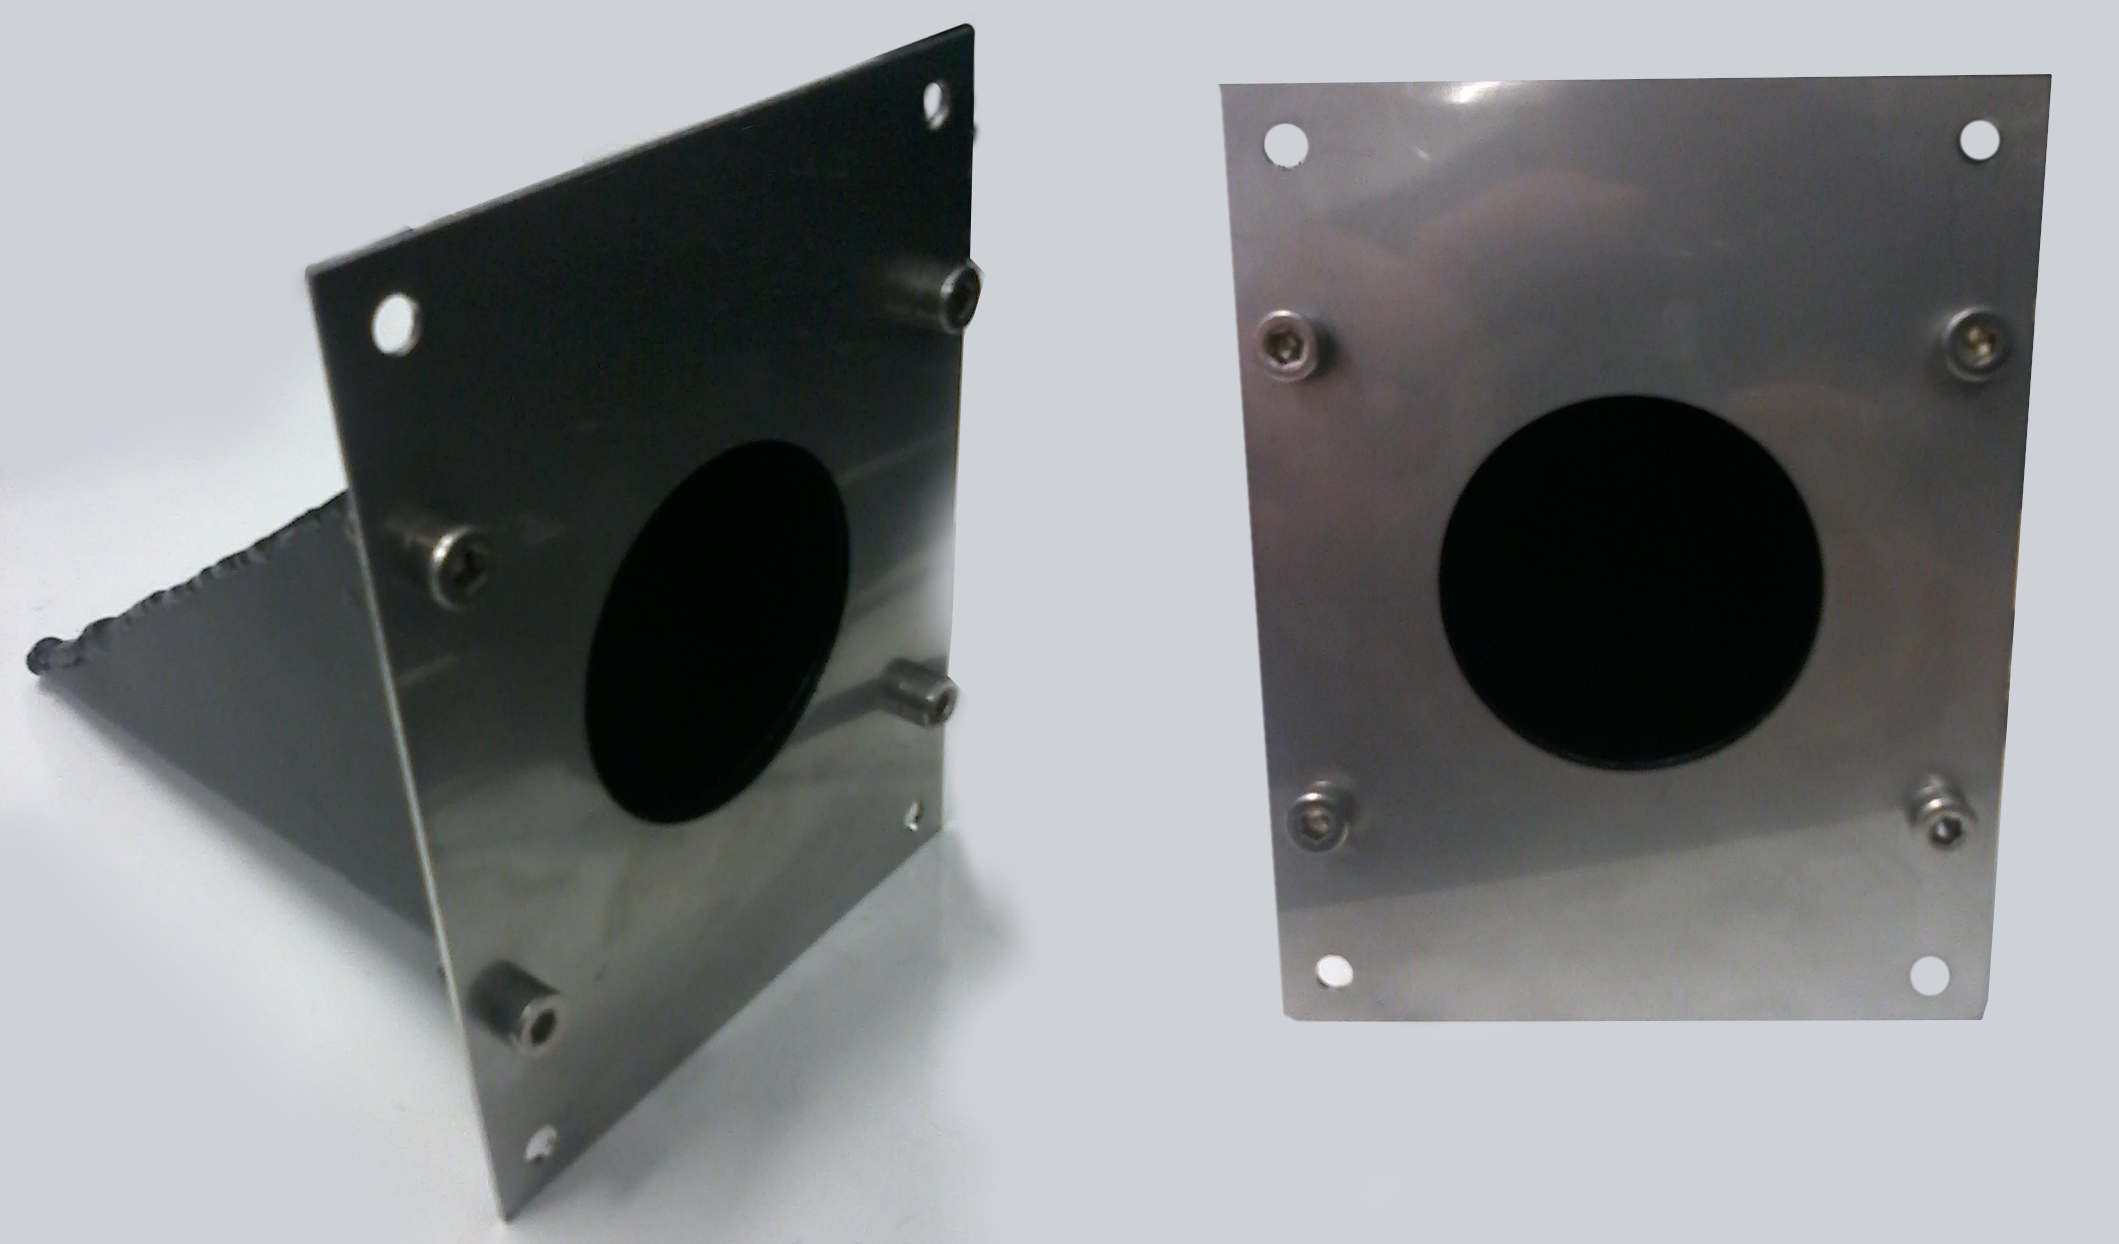
\includegraphics[width=0.7\linewidth]{Figures/4.Chapter/blackbody.png}
\caption{Completed Blackbody}
\label{fig:blkbdy}
\end{figure}

\par The final setup, after all parts were mounted can be seen in Figure \ref{fig:bbcs}. With this setup, it is possible to collect and control temperature values, and correlate them with the camera data. This device was used to perform 2 different calibrations, that will be explained further ahead in this chapter. \\

\begin{figure}[h]
\centering
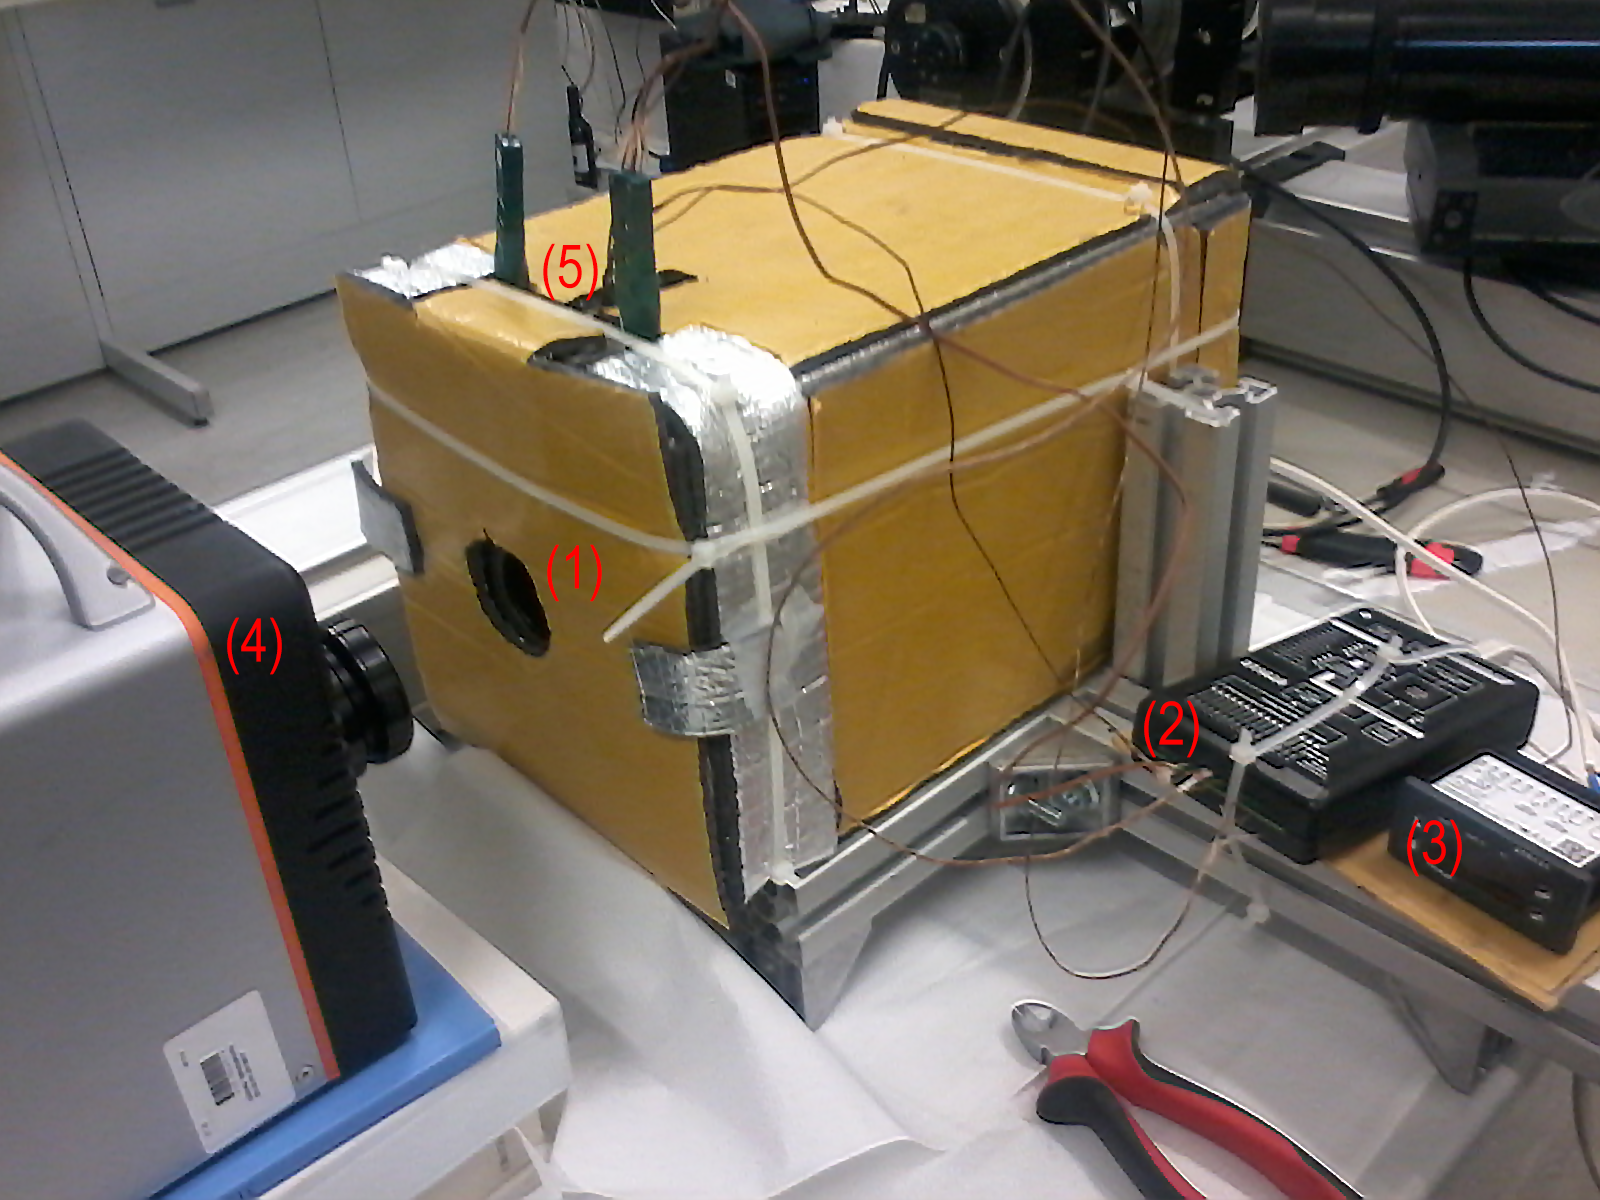
\includegraphics[width=0.7\linewidth]{Figures/4.Chapter/complete.png}
\caption{Completed Blackbody Calibration Source: (1) Blackbody cavity; (2) Data Aquisition Board; (3) PID controller; (4) IR Camera; (5) Thermocouples (one connected to the PID, the others to the Data Aquisition Board)}
\label{fig:bbcs}
\end{figure}

\section{Calibration process}

\par A number of steps must be followed before starting the actual calibration process:
\begin{itemize}
\item Fill the device with oil.
\item Connect the thermocouples to the Data Aquisition Board and to the PID Controller.
\item Turn on the IR Camera and start both its software (Xeneth) and the board software (QuickDAQ).
\item Define an adequate integration time to the desired temperature interval.
\item Perform an offset calibration with the camera software.
\end{itemize}

\par Now the camera can be calibrated using the software’s calibration feature or the custom made process proposed here. While in the software calibration is automatic, in the custom made calibration the average ADU of the selected region needs to be registered along with the average temperature read by the sensors on an Excel sheet. \\

\begin{figure}[h]
\centering
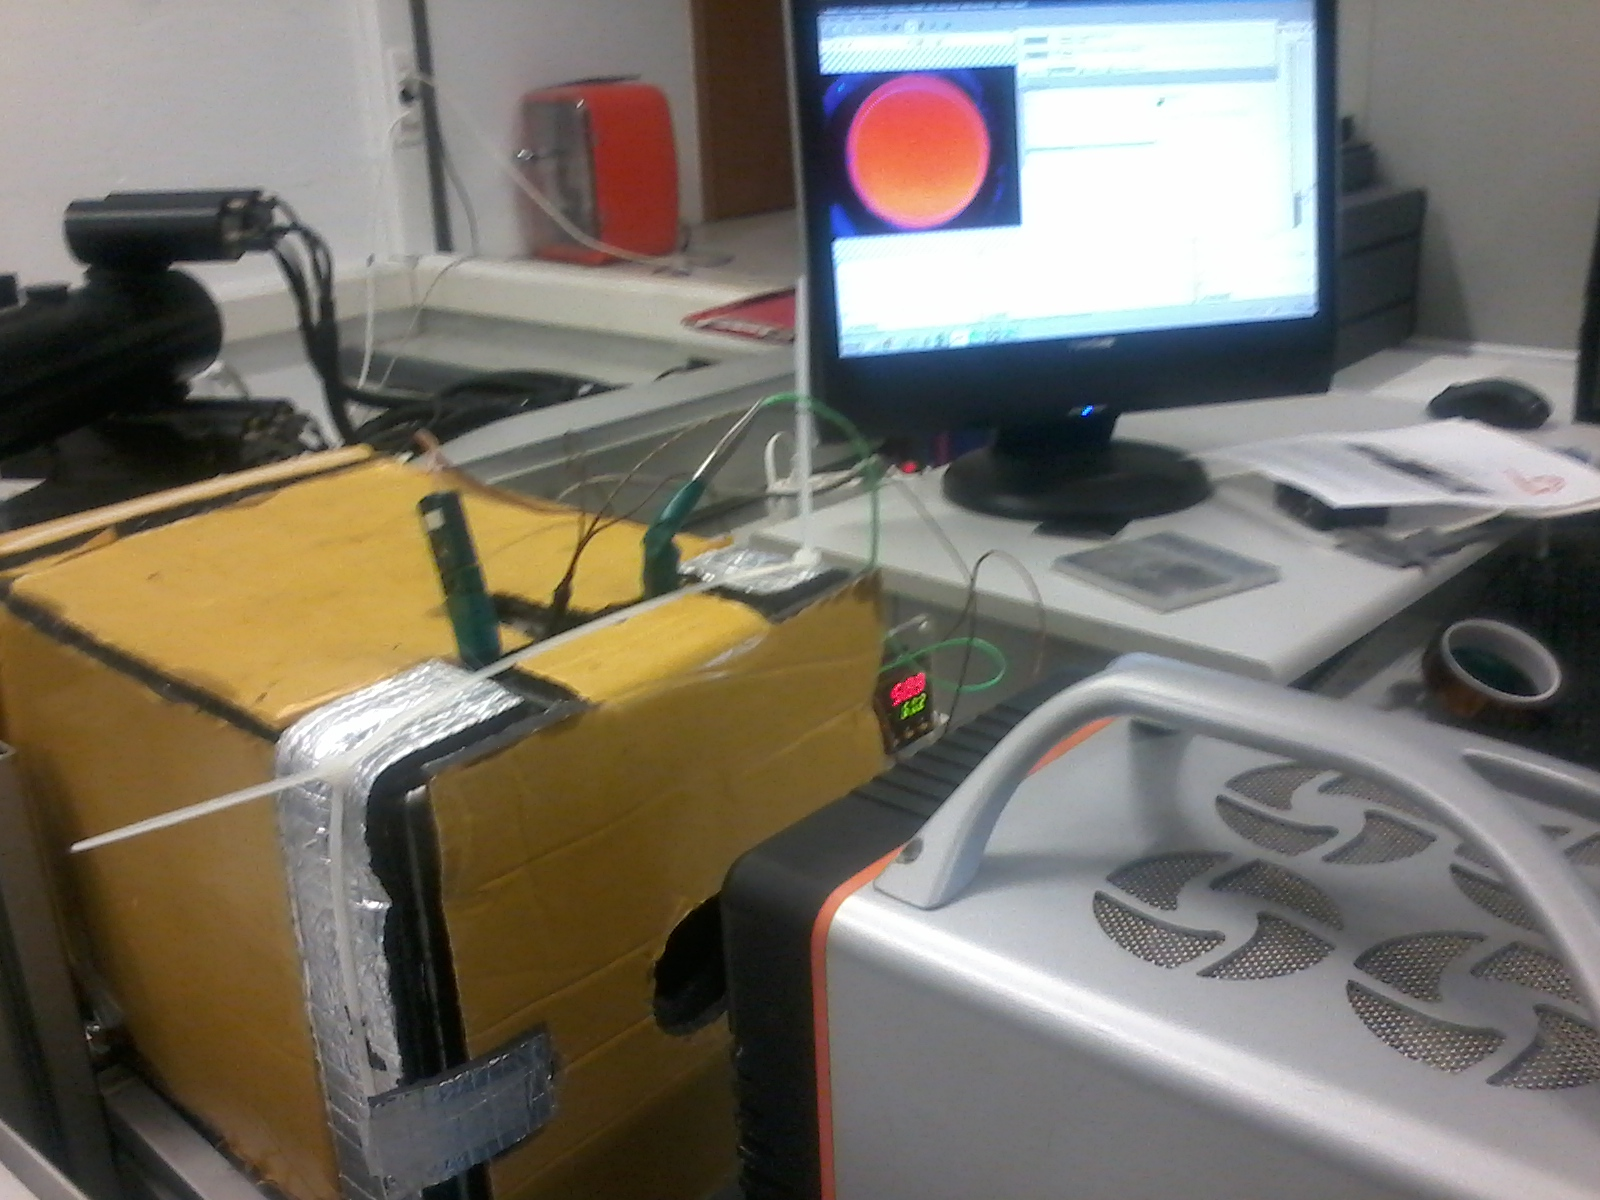
\includegraphics[width=0.55\linewidth]{Figures/4.Chapter/calibinprog.jpg}
\caption{Calibration Instalation in Function}
\label{fig:calibinprog}
\end{figure}

\begin{figure}[h]
\centering
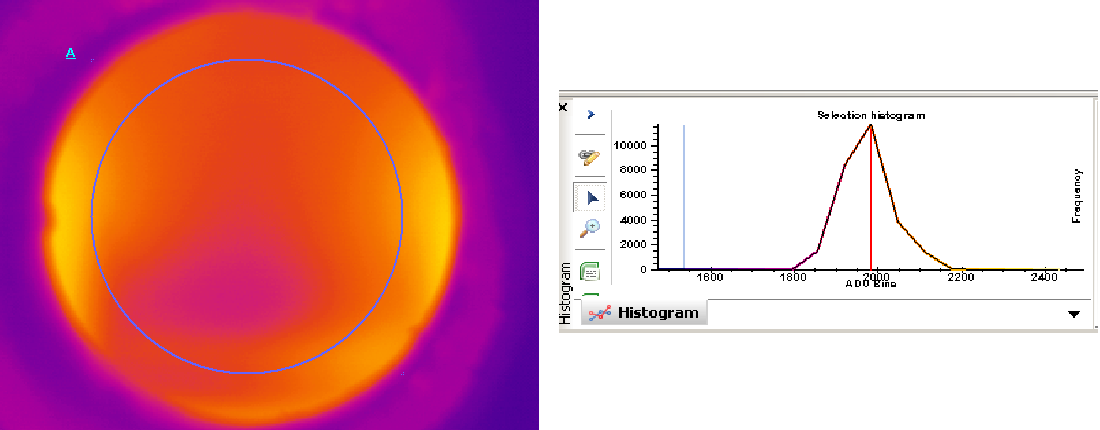
\includegraphics[width=1\linewidth]{Figures/4.Chapter/ex11.png}
\caption{Blackbody thermal image and its respective histogram}
\label{fig:ex1}
\end{figure}

\par The overall setup for the custom made calibration is assembled in Figure \ref{fig:calibinprog}. The desired temperature is set and is gradually increased in 10ºC/20ºC increments to have a wide range of temperatures (up to 130ºC).Each set temperature must stabilize until the image of the cavity shows a uniform temperature within the entire selected area. For instance, Fig. 4.11 shows that the edges of the cavity are hotter than the remaining cavity region. This is due to different thermal properties of the materials used to assemble the cavity blackbody.\\

\par This problem is solved by the PID controller. To understand this, one can summarize the way the PID is working to control the temperature as follows: the input target temperature of the PID is compared with that read by the thermocouple connected to the controller, and it turns on and off the resistance to keep the temperature constant within a desired range (+/-1ºC). The resistance is turned of just before the oil is at the desired temperature in order to account for thermal inertia of the device and for the delays in the controller.\\

\begin{figure}[h]
\centering
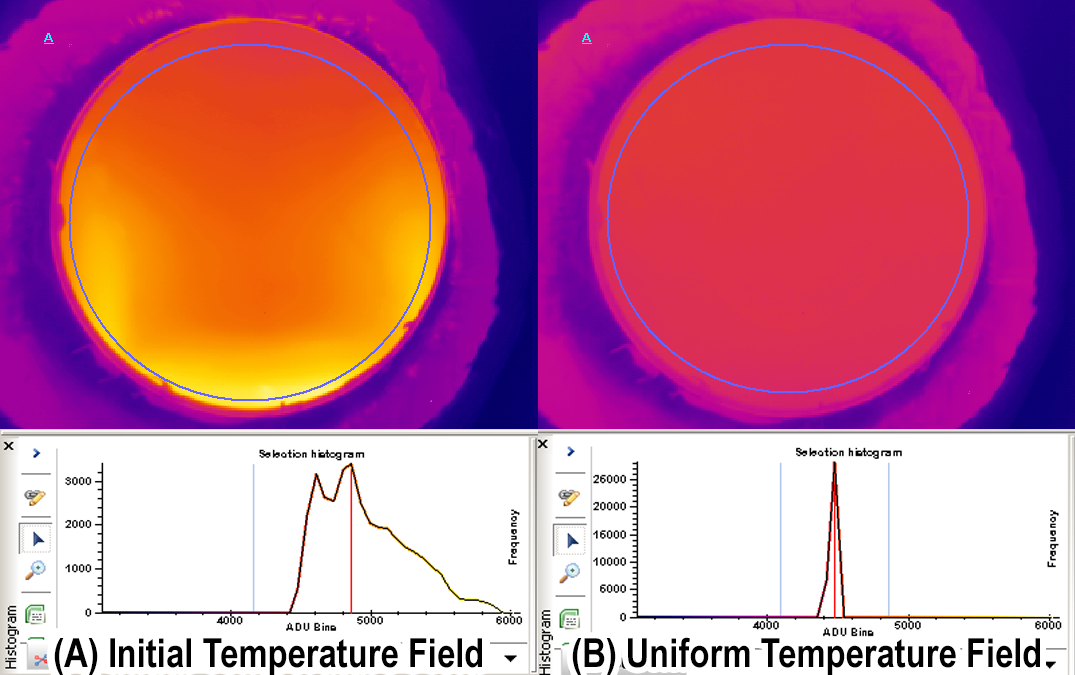
\includegraphics[width=0.9\linewidth]{Figures/4.Chapter/ex2.png}
\caption{Calibration example: initial temperature field, and uniform temperature field (after $\approx$5 min)}
\label{fig:ex2}
\end{figure}

\par So, when the electrical resistance is off, the thermal inertia of the oil and the good insulation of the Blackbody device allow reaching a uniform temperature in the cavity, as the device cools down. This can be clearly seen in Fig. 4.12.
The histograms show perfectly the desired conditions (the peak on the right histogram contrasting with the wider dispersion of values in the left histogram in Figure \ref{fig:ex2}). \\

\par To see what temperature corresponds to the averaged ADU value, an average of the surface thermocouple read temperatures in time was taken, with the help of the software QuickDAQ, which allows to take a data sample for a fixed amount of time. This is used to make the average between all the surface thermocouples connected to the board and the value shown in the PID. This final average is then the input for the software calibration or saved with the ADU in an excel for the second method. \\

\subsection{Software Calibration}

\par The Xenics' software has a camera calibration wizard (in which the offset calibration feature is included) that automatically correlates the ADU's with the temperature measured. The feature described is called "Temperature Calibration (Plank)" and can be seen in Figure \ref{fig:plankcalib}. In the shown interface, the user can input the temperature measured by the thermocouples in the field (a), and then add the read value with button (b). It will then add a point, to the table at the left and draw in on a graph bellow. This point has the given temperature, and the ADU measured with a spatial average of a small rectangular area in the center of the image. \\

\begin{figure}[h]
\centering
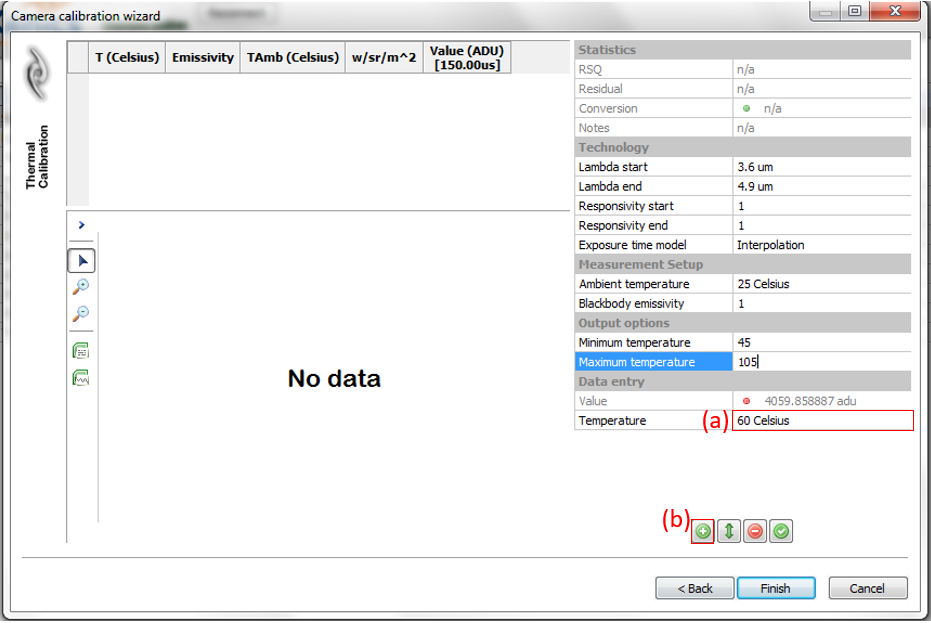
\includegraphics[width=0.7\linewidth]{Figures/4.Chapter/plankcalib.png}
\caption{Xeneth's software - Temperature Calibration (Plank)}
\label{fig:plankcalib}
\end{figure}

\par In the first calibration, this method was tried but because the temperature and respective measured ADU are shown it didn't invalidate the possibility to use them in the second method, our custom made calibration. In this attempt an integration time of 450 was used. The final table and graphic can be seen in Figure \ref{fig:calib}. On the table labeled as (a) one can see 5 columns. The first and last columns depict the read values of temperature and ADU, respectively. The second and third columns show the ambient temperature and emissivity which are actually irrelevant for the present calibration as one assumes the cavity to be a perfect blackbody, so the ambient temperature won't be used in this calibration. The fourth column is a variable, which depends on the input temperature, that the software uses to convert, together with the other inputs, the temperature, in a quantity called "Soaled Radiance", represented in the x axys of graph (b) in Figure \ref{fig:calib}. This variable is not explained in the manual, nor its relation with the temperature. This was one of the disadvantages of this method mainly because the software creates the "Soaled Radiance" value out of it, and it is supposed to maintain a proportional relation with the ADU's so the calibration correlation is linear. But as it is noticeable in the graph, the values do not follow the line that closely, which caused a significant deviation. \\

\par Having this variable and the "Soaled Radiance" unexplained, the only option was to take these values and use them in the other method. Another reason is that this method does a linear correlation. This may only be a vague assumption or a rough approximation, and because even if the origin of these variables was known, there would be no way to validate that linear relation. \\

\par In the end, the software creates a calibration conversion that can be selected when it is opened and used to take the data directly in Celsius. This calibration file can only be used for the specified integration time. In Figure \ref{fig:calib} it's possible to see how the software approximates linearly (green line) the measured points (red line). Because this calibration didn't match the experimental values as close as desired, when the newly created calibration pack was tested it didn't work properly, so the second type of calibration was made.\\

\begin{figure}[h]
\centering
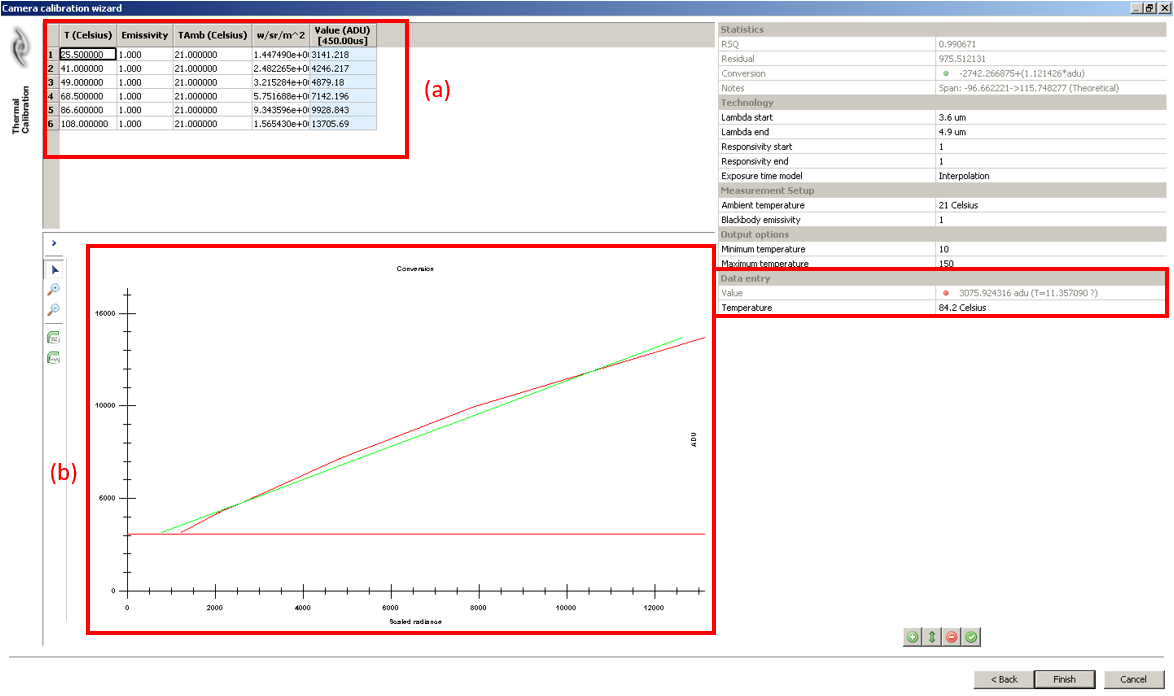
\includegraphics[width=0.7\linewidth]{Figures/4.Chapter/calibracao.png}
\caption{Complete Temperature Calibration (Plank)}
\label{fig:calib}
\end{figure}

\subsection{Proposed Calibration}
\par Being unable to trust the calibration method provided by the camera software, a custom made method was developed. In this method the calibration results (average ADU in a selected region) are taken directly from the software, without using the software's Calibration Wizard. They're saved in an Microsoft Excel sheet together with the average temperature read by the thermocouples. With this method the results have to be taken raw from the software and then process them with the MATLAB code that was made just for this purpose. A whole explanation of the process will be given in the next section, leaving in this section a general outline of the proposed method.\\

\par The process of data aquisition for the calibration is similar to the previous calibration. The main difference in this method is the absence of the Calibration Wizard. Instead, the Selection Panel (described in \ref{software}) is used to gather the average measured ADU of a circular area, similar to what can be seen in Figure \ref{fig:ex2}. There are several advantages in this method, one being that it was now possible to adjust the temperature range (the Calibration Wizard didn't allow it), and better understand when the image saturates. Another advantage is the fact that it is possible to change integration time. \\

\par In Microsoft Excel, the measured temperatures are converted into the radiated energy using equation \ref{eq:6} (and considering the object perfectly black) and plotted against the ADU. Then Microsoft Excel's trending line function is used to extract a polynomial curve that will best approximate the data gathered in the experiments. The second and third degree polynomial approximations were compared, but in the end the third degree polynomial. This option took longer to process but the end result was significantly closer to the experimental results. \\

\par With the extracted curve a MATLAB code was made to calibrate the videos. The raw data video data (in ADU) matrix is the input of this function. This matrix has the value for every pixel in every frame, and point by point is solving the following equation:

\begin{equation}
A \times W_{tot}^3 + B \times W_{tot}^2 + C \times W_{tot} + D = ADU_{pixel}
\end{equation}

in which A,B,C and D are the coefficients of the calculated polynomial curve, $ADU_{pixel}$ is the pixel ADU value and $W_{tot}$ is the wanted radiated energy. Using this radiated energy value, the pixel temperature is calculated using equation \ref{eq:7}. The end result is a matrix with all the temperatures.

\subsection{Calibration Process Details}

\par One important fact about the designed calibration procedure is that it took a whole day to complete. This is due to the fact that there was no refrigeration system and the liquid had to cool at room temperature. Also the overheating of the device often leads to leakages due to material expansion and break down. This problem, which often would not allow to repeat the calibration process in a regular way, took some time to address.\\

\par Two calibrations were made during this work. The first was made using the software at the fixed integration time of it=450us. The second was made using the proposed method for the integration times of it=450us and it=200us. With the integration time of it=450us the image would saturate at around 108ºC, so the correspondent results weren't suited for the experiments represented here which would reach higher temperatures. \\

\par The results of the calibrations is shown in Table \ref{tab:calibration}. Since the results were taken for both calibrations at $it=450us$ we can use them to prove the method's consistency. The comparison is presented Figure \ref{fig:calibplot}.  \\

\begin{table}[h]
\centering
\caption{Calibration Results}
\label{tab:calibration}
\begin{tabular}{ccccccccc}
\toprule
\multicolumn{3}{c}{Calibration 1}       &  & \multicolumn{5}{c}{Calibration 2}                                    \\ 
\cmidrule[0.4pt](r{0.125em}){1-3}%
\cmidrule[0.4pt](r{0.125em}){5-9}%
         & \multicolumn{2}{c}{it=450us} &  &        & \multicolumn{2}{c}{it=450us} & \multicolumn{2}{c}{it=200us} \\
\cmidrule[0.4pt](r{0.125em}){2-3}%
\cmidrule[0.4pt](r{0.125em}){6-7}%
\cmidrule[0.4pt](r{0.125em}){8-9}%
T(ºC)  & ADU         & $W_{tot}(W/m^2)$      &  & T(ºC)& ADU         & $W_{tot}(W/m^2)$      & ADU         & $W_{tot}(W/m^2)$      \\
\cmidrule[0.4pt](r{0.125em}){1-3}%
\cmidrule[0.4pt](r{0.125em}){5-9}%
25.5     & 3141        & 450.1533       &  & 25.46  & 3200        & 449.912        & 1645        & 449.912        \\
41       & 4246        & 551.1904       &  & 34.5   & 3794        & 506.9481       & 1900        & 506.9481       \\
49       & 4879        & 609.5461       &  & 44.28  & 4666        & 574.5844       & 2285        & 574.5844       \\
68.5     & 7142        & 771.1625       &  & 62.27  & 6287        & 716.4103       & 3021        & 716.4103       \\
86.6     & 9928        & 948.1167       &  & 75.76  & 8270        & 838.8605       & 3890        & 838.8605       \\
108      & SAT         & SAT            &  & 84.33  & 9827        & 924.4022       & 4596        & 924.4022       \\
         &             &                &  & 94.54  & 12094       & 1034.669       & 5586        & 1034.669       \\
         &             &                &  & 103.67 & 14078       & 1141.372       & 6690        & 1141.372       \\
         &             &                &  & 114.39 & SAT         & SAT            & 8139        & 1276.958       \\
         &             &                &  & 125.74 & SAT         & SAT            & 9885        & 1433.317     \\ \bottomrule
\end{tabular}
\end{table}

\begin{figure}[h]
\centering
\begin{tikzpicture}
\begin{axis}[
	title = {Iteration Time = 450us},
    tick label style={font=\scriptsize},
    legend style={font=\scriptsize,/tikz/column 2/.style={column sep=5pt},},
    legend columns=2,
    legend cell align=left,
	legend pos =south east,
    grid=major, % Display a grid
    grid style={dashed,gray!30}, % Set the style
    xlabel={ADU},
    ylabel={$W_{tot} (W/m^2)$}, 
    ymin = 400, ymax = 1200,
    %ytick={300,325,350,375,400,425,450,475,500,525},
    %yticklabels={300,325,350,375,400,425,450,475,500,525},
    xmin = 3000, xmax = 15000,
    xtick={0,1000,...,15000},
    xticklabel style={
        /pgf/number format/fixed,
        /pgf/number format/precision=5},
	scaled x ticks=false,
    width=\textwidth, height=9cm,
    %legend entries={Experimental,Computational, $264 W/m^{2}$,$807 W/m^{2}$,$2031 W/m^{2}$,$3636 W/m^{2}$}
    ]

% \addlegendimage{only marks, mark=square*,black}
% \addlegendimage{only marks, mark=x      ,black}
% \addlegendimage{only marks, mark=*      ,blue}
% \addlegendimage{only marks, mark=*      ,red}
% \addlegendimage{only marks, mark=*      ,brown}
% \addlegendimage{only marks, mark=*      ,black}


%-------------------------------------------------------------
%Experimental ------------------------------------------------
%-------------------------------------------------------------

\addplot+[only marks,mark=square*,blue] % 264 experimental
coordinates {(	3141	,	450.1532612	)
(	4246	,	551.1904079	)
(	4879	,	609.5460842	)
(	7142	,	771.1624794	)
(	9928	,	948.1166888	)
};
\addplot+[only marks,mark=square*,red]
coordinates{(	3200	,	449.9120215	)
(	3794	,	506.9481463	)
(	4666	,	574.5844207	)
(	6287	,	716.4103256	)
(	8270	,	838.8604805	)
(	9827	,	924.4022127	)
(	12094	,	1034.669156	)
(	14078	,	1141.371929	)};
\legend{Calibration 1, Calibration 2}

\end{axis}
\end{tikzpicture}
\caption{Comparison of the two calibrations at it=450us}
\label{fig:calibplot}
\end{figure}

\par Next, the $it=200us$ data has to be plotted, and a trending line calculated. The data with the correspondent trending line can be seen in Figure \ref{fig:calibcurve}. The equation that is represented in the plot is the one used in the calibration code. \\

\begin{figure}[h]
\centering
\begin{tikzpicture}
\begin{axis}[
	title = {Iteration Time = 200us},
    tick label style={font=\scriptsize},
    legend style={font=\scriptsize,/tikz/column 2/.style={column sep=5pt},},
    %legend columns=2,
    legend cell align=left,
	legend pos =south east,
    grid=major, % Display a grid
    grid style={dashed,gray!30}, % Set the style
    xlabel={$W_{tot} (W/m^2)$},
    ylabel={ADU}, 
    ymin = 0, ymax = 11200,
    %ytick={300,325,350,375,400,425,450,475,500,525},
    %yticklabels={300,325,350,375,400,425,450,475,500,525},
    xmin = 400, xmax = 1500,
    ytick={0,1600,...,11200},
    yticklabel style={
        /pgf/number format/fixed,
        /pgf/number format/precision=5},
	scaled y ticks=false,
    width=\textwidth, height=9cm,
    ]
\addplot+[only marks,mark=square*,blue]
coordinates {(	449.9120215	,	1645	)
(	506.9481463	,	1900	)
(	574.5844207	,	2285	)
(	716.4103256	,	3021	)
(	838.8604805	,	3890	)
(	924.4022127	,	4596	)
(	1034.669156	,	5586	)
(	1141.371929	,	6690	)
(	1276.958202	,	8139	)
(	1433.317083	,	9885	)
};
\addlegendentry{Calibration Results}
\addplot[
    domain=450:1430, 
    samples=100, 
    color=red,
]{0.00847*x^2 - 0.00000149*x^3 - 3.27*x + 1570};
\addlegendentry{$-1.49\times 10^{-6}x^3 + 8.47\times 10^{-3}x^2 - 3.27x + 1570$}
\end{axis}
\end{tikzpicture}
\caption{Comparison of the two calibrations at it=450us}
\label{fig:calibcurve}
\end{figure}

\par The generated code is used to transform every video from ADU values to Celsius, and works only for the selected integration time. The code can also be easily adapted to the integration time of 450us. This code can be seen in Appendix \ref{ap:a}. \\

\clearpage

\section{Data Processing Methods}
\par The collected images, without any sort of treatment, have some random noise and unwanted patterns of noise. While the noise source is usually small differences in sensitivity or calibration of the sensors, the patterned noise has it's origin mainly on the software processing. A temperature difference is always noticeable inside the region of interest. This cannot be solved so, to accurately evaluate the results, a background remove has to be performed. This also helps removing some background noise. \\

\par To be treated, the video needs to be imported to avi format, in an 8 bit, grey scale format. In MATLAB, the video is divided into frames and the grey scale value transformed to temperature, considering the temperature or ADU scale it was imported with. After this, the calibration is applied and finally the filters. In the end, the results are extracted as a MATLAB file with all values and a txt with the results from the center to the radius of the droplet with a plot option.

\subsection{Patterned Noise}

\par The origin of this type of noise was detected in the software's zoom function. It can result in significant errors. At constant temperature the results showed that the  difference between pixels side by side was 1ºC. To remove this, a filter was made that would add and subtract 0.5ºC alternately. The generated pattern and the effect of the filter can be seen in Figure \ref{fig:chess}.

\begin{figure}[h]
\centering
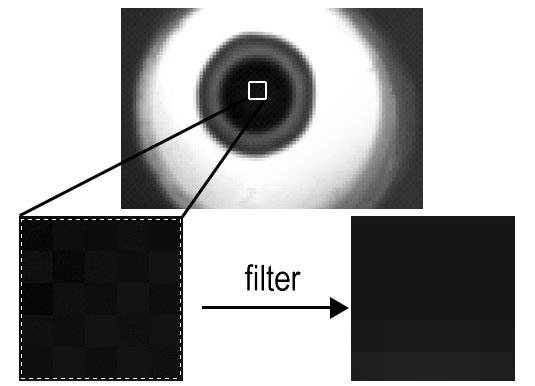
\includegraphics[width=0.5\linewidth]{Figures/4.Chapter/chess2.png}\\
\subfigure{
\begin{tikzpicture}
\begin{axis}[
	width=0.5\linewidth,
    height=0.3\linewidth,
	%title = {Unprocessed Results},
    tick label style={font=\scriptsize},
    legend style={font=\scriptsize,/tikz/column 2/.style={column sep=5pt},},
    %legend columns=2,
    legend cell align=left,
	legend pos =south east,
    grid=major, % Display a grid
    grid style={dashed,gray!30}, % Set the style
    xlabel={pixel},
    ylabel={T (ºC)}, 
    %ymin = 0, ymax = 11200,
    %ytick={300,325,350,375,400,425,450,475,500,525},
    %yticklabels={300,325,350,375,400,425,450,475,500,525},
    %xmin = 400, xmax = 1500,
    %ytick={0,1600,...,11200},
    %yticklabel style={
    %    /pgf/number format/fixed,
    %    /pgf/number format/precision=5},
	%scaled y ticks=false,
    ]
\addplot+[mark=square*,blue]
coordinates {(	1	,	29.23	)
(	2	,	32	)
(	3	,	32.7	)
(	4	,	34.09	)
(	5	,	33.05	)
(	6	,	34.09	)
(	7	,	32.7	)
(	8	,	34.09	)
(	9	,	34.09	)
(	10	,	37.9	)
(	11	,	41.03	)
(	12	,	44.84	)
(	13	,	44.15	)
(	14	,	43.45	)
(	15	,	40.33	)
};
%\addlegendentry{}
\end{axis}
\end{tikzpicture}
}%
\subfigure{
\begin{tikzpicture}
\begin{axis}[
	width=0.5\linewidth,
    height=0.3\linewidth,
	%title = {Processed Results},
    tick label style={font=\scriptsize},
    legend style={font=\scriptsize,/tikz/column 2/.style={column sep=5pt},},
    %legend columns=2,
    legend cell align=left,
	legend pos =south east,
    grid=major, % Display a grid
    grid style={dashed,gray!30}, % Set the style
    xlabel={pixel},
    ylabel={T (ºC)}, 
    %ymin = 0, ymax = 11200,
    %ytick={300,325,350,375,400,425,450,475,500,525},
    %yticklabels={300,325,350,375,400,425,450,475,500,525},
    %xmin = 400, xmax = 1500,
    %ytick={0,1600,...,11200},
    %yticklabel style={
    %    /pgf/number format/fixed,
    %    /pgf/number format/precision=5},
	%scaled y ticks=false,
    ]
\addplot+[mark=square*,blue]
coordinates {(	1	,	29.73	)
(	2	,	31.5	)
(	3	,	33.2	)
(	4	,	33.59	)
(	5	,	33.55	)
(	6	,	33.59	)
(	7	,	33.2	)
(	8	,	33.59	)
(	9	,	34.59	)
(	10	,	37.4	)
(	11	,	41.53	)
(	12	,	44.34	)
(	13	,	44.65	)
(	14	,	42.95	)
(	15	,	40.83	)
};
%\addlegendentry{}
\end{axis}
\end{tikzpicture}
}
\caption{The effect of the filter in both the image and a line of point temperature values}
\label{fig:chess}
\end{figure}


\subsection{Median Filter}

\par This filter has the potential to remove random bad pixels noise from the picture. This filter is a MATLAB function that outputs the median of a 3-by-3 neighborhood of the input pixel. With this simple filter the image can be greatly improved as shown in Figure \ref{fig:median}. On the right there's the image without the filter and on the left the treated image.

\begin{figure}[h]
\centering
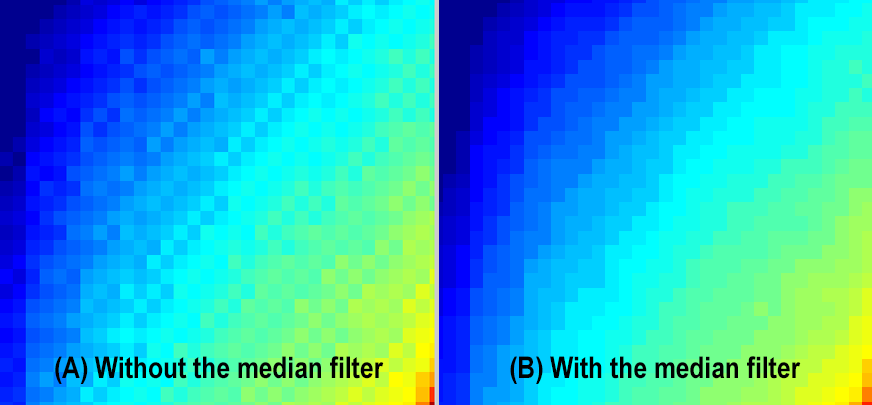
\includegraphics[width=0.6\linewidth]{Figures/4.Chapter/median.png}
\caption{Median filter effect}
\label{fig:median}
\end{figure}

\subsection{Background Filter}
\par The background filter serves the function of eliminating any problems related with the optics of the camera and to equalize the temperature field. Two different ways to do it were thought. Two MATLAB codes were made and tested. The first one is the simple way and is shown in Equation \ref{eq:bkg}. The variable $vid$ is the matrix with the temperature value for every pixel in every frame, $avTemp$ is the average temperature in the center of the hole and $t_n$ is the number of the analyzed frame.
\begin{equation}\label{eq:bkg}
vid^{*}(x,y,t_n)=vid(x,y,t_n)-vid(x,y,1)+avTemp
\end{equation}
\par The second one is a weighted background removal and we can see it in Equation \ref{eq:pbkg}. The variables bear the same meaning, but has to be done for each pixel ($x_p,y_p$). Only the code for the latter can be seen in Appendix \ref{ap:b} as the code is similar in both cases. 
\begin{equation}\label{eq:pbkg}
vid^{*}(x_p,y_p,t_n)=\frac{vid(x_p,y_p,t_n)-vid(x_p,y_p,1)}{vid(x_p,y_p,1)}avTemp+avTemp
\end{equation}
\begin{figure}[h]
\centering
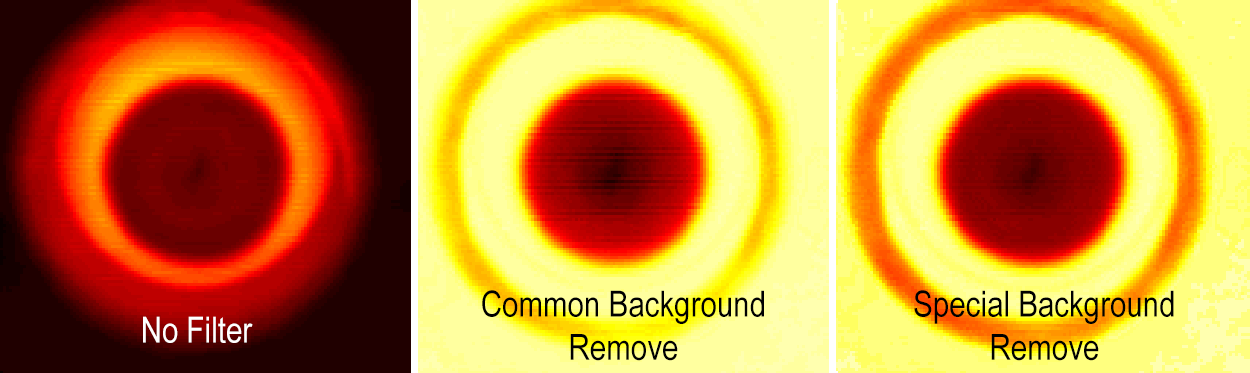
\includegraphics[width=0.8\linewidth]{Figures/4.Chapter/bkg.png}
\caption{Background filter effect}
\label{fig:bkg}
\end{figure}

\subsection{Heat Flux computation}

\par To evaluate and compare the heat removal capacity of the system it is very important to compute the heat flux and cooling effectiveness, mentioned in Section \ref{sec:heat}. This was also made with the help of a MATLAB code, that can be seen in Appendix \ref{ap:c} and \ref{ap:d}.\\
\par Starting with the computation of the heat flux the code is a discretization of Equation \ref{eq:heatf}. This equation can be divided in three terms: the provided heat flux, the spacial term and the temporal term. This problem was addressed as being axisymmetric, so the spatial derivative becomes a one-dimensional problem. To address the second order derivative in the spatial term a backward discretization with first order precision was applied:\\
\begin{equation}
\frac{{\partial}^2 T}{\partial r^2} \approx \frac{T_i-2T_{i-1}+T_{i-2}}{\Delta r^2}
\end{equation}

\par The temporal term has a first order derivative, that was addressed the same way and discretized using a first order precision backward method:

\begin{equation}
\frac{{\partial} T}{\partial t} \approx \frac{T_t-T_{t-1}}{\Delta t}
\end{equation}

\par To compute the cooling effectiveness, one has to solve Equation \ref{eq:epsilon}. This means integrating the flux both in time and space. This integration was approximated using the trapezoidal integration method. Starting with the spatial integration first:

\begin{equation}
\int_A q'' \; dA = \int_\theta \int_r r \times q''(r) dr d\phi
\end{equation}

using integration by parts this integral and assuming the flux to be axisymetric (no variation in $\theta$) one can write the integral as:

\begin{equation}
\int_\theta \int_r r \times q''(r) dr d\theta = \bigg( r \int_r q''(r) dr - \int_r \cancelto{1}{\frac{d}{dr}r} \int_r q''(r) dr dr \bigg) \times 2 \pi
\end{equation}

\par To compute the integral now, one just needs to apply an trapezoidal approximation:

\begin{equation}
\int_r q''(r) dr \approx \frac{q''(r)+q''(r+1)}{2} \times \Delta r
\end{equation}
\begin{equation}
\int_r \int_r q''(r) dr dr = \frac{q''(r)+ q''(r+1) + q''(r+1)+q''(r+2)}{4} \times \Delta r^2
\end{equation}

\par Finally, the temporal integral was addressed similarly:
\begin{equation}
\int_t P_{diss}(t) dt = \frac{P_{diss}(t)+ P_{diss}(t+1)}{2} \times \Delta t
\end{equation}
\par This integral is solved for every timestep so that is possible to obtain a graphic of the time evolution for this parameter.


\cleardoublepage
\chapter{Experimental Results}
\label{cap:results}


\section{Indroduction}

\par This chapter explores the use of the IR camera (after taking the calibration procedures) to describe the heat transfer occurring at droplet wall interactions. The analysis focus on discussing the potential and limitations of this technique. Additionally the heat transfer processes are investigated, addressing the effect of liquid properties, surface wettability and surface temperature 

\section{Side View}

\par This experiment served as an introductory case study to get familiar with the camera characteristics. As stated before, the geometric implications of the droplet shape in radiation prevent the extraction of quantitative results, as well as the transmissivity of the liquid to infrared, although it's close to 0 for water.\\
\par This experiment addressed two different impact velocities: 2 m/s and 0.8 m/s, and three initial foil temperatures: 60ºC, 100ºC and 110ºC. The results obtained in this configuration are shown in Figure \ref{fig:hexp} and Figure \ref{fig:hexp2}, mainly illustrative results. In this figure, the x axis represents the distance between the bottom of the droplet to its top. These results show that for the same impact velocity, the temperature gradient in the droplet, from the surface to the top, evolves similarly along time irrespective of the surface temperature. The temperature at the liquid-solid interface is naturally higher than that on the bulk of the droplet. At early stages the temperature at the interface is also lower than at later stages of spreading, when the thickness of the lamella becomes thinner. As for the impact velocity comparison, the results show a bigger temperature increase at the lamella's base for the higher impact velocity profile.

\begin{figure}[h]
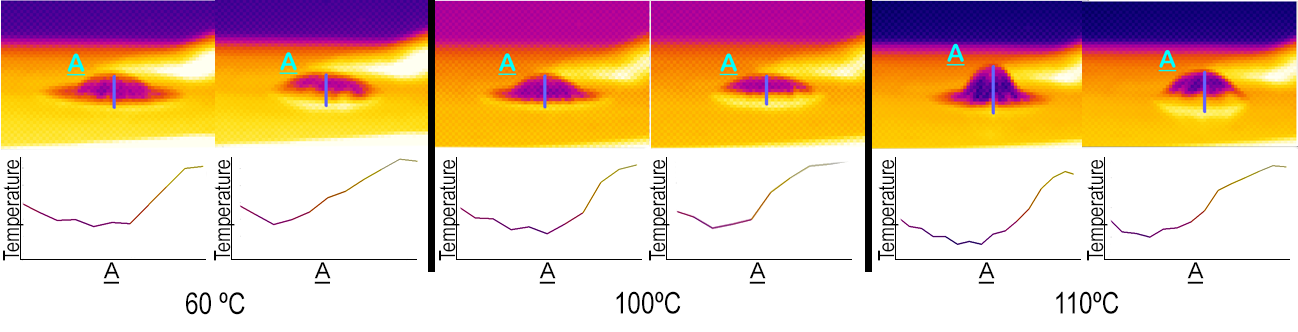
\includegraphics[width=1\linewidth]{Figures/5.Chapter/hexp.png}
\caption{Side view of the water droplets impacting the hydrophilic foil at 2 m/s: spreading and receding phases}
\label{fig:hexp}
\end{figure}

\begin{figure}[h]
\centering
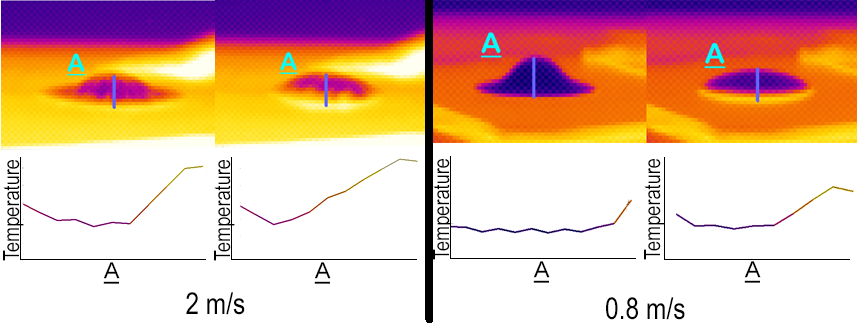
\includegraphics[width=0.66\linewidth]{Figures/5.Chapter/hexp2.png}
\caption{Side view Results for 60ºC during the spreading and receding phases}
\label{fig:hexp2}
\end{figure}

\section{Bottom View}

\par The images obtained in this configuration are mainly bidimensional temperature maps of the area on the surface corresponding to the area that is wetted by the droplet. From this map one can obtain the distribution of the temperature along the droplet radius for small time steps. Further post processing of the collected data was used to compute the heat flux and cooling effectiveness (as explained in Chapter 2), to compare the results obtained in the various experimental conditions. The connection between the high-speed images, temperature map and temperature plot is depicted Figure \ref{fig:hexp}.\\

\begin{figure}[h]
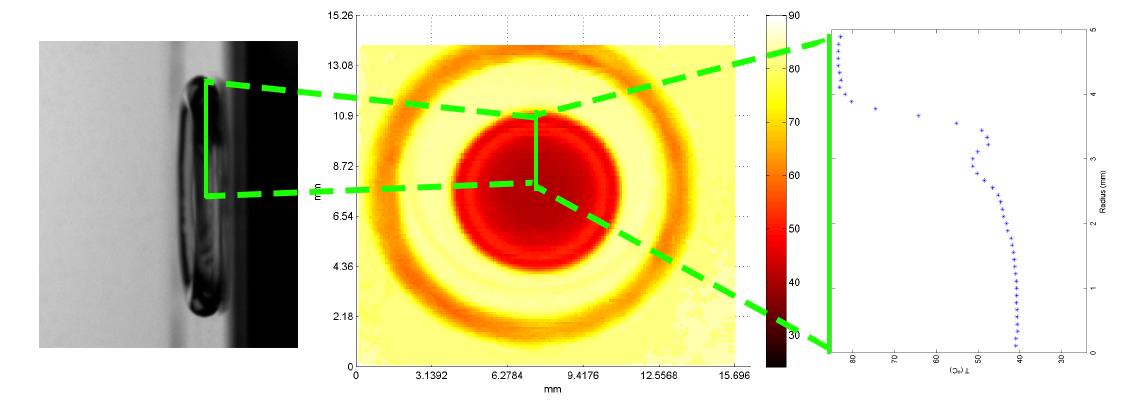
\includegraphics[width=1\linewidth]{Figures/5.Chapter/example.png}
\caption{Example of the results representation}
\label{fig:hexp}
\end{figure}

\par In fact various conditions were tested, namely two different impact velocities, 0.8 m/s and 2 m/s, and four initial foil temperature values, for conditions before and after the saturation point, 60ºC, 80ºC, 100ºC and 110ºC. Additionally, two different wettability conditions were compared, namely using the hydrophilic foil and the super-hydrophobic, coated foil. Finally, tests were also performed with two liquids: water and ethanol. As for each of the conditions, 5 different experiments were made, so that the repeatability of the tests could be confirmed. In Figure \ref{fig:repeat} the repeatability of these tests can be seen with the example of the 60ºC results for 2 m/s.\\

\begin{figure}[h]
\centering
\begin{tikzpicture}
\begin{axis}[
	title = {2 m/s || 60 ºC || $T_{amb}=24$},
    tick label style={font=\scriptsize},
    legend style={font=\scriptsize,/tikz/column 2/.style={column sep=5pt},},
    %legend columns=2,
    legend cell align=left,
	legend pos =south east,
    grid=major, % Display a grid
    grid style={dashed,gray!30}, % Set the style
    xlabel={Droplet Radius (mm)},
    ylabel={T (ºC)}, 
    ymin = 25, ymax = 65,
    ytick={30,35,...,120},
    %yticklabels={300,325,350,375,400,425,450,475,500,525},
    xmin = 0, xmax = 7,
    %ytick={0,1600,...,11200},
    %yticklabel style={
    %    /pgf/number format/fixed,
    %    /pgf/number format/precision=5},
	%scaled y ticks=false,
    width=1\textwidth, 
    height=7cm,
    cycle list name= color
    ]
\addplot+[dashed]
coordinates {(	0	,	30.48	)
(	0.11	,	29.97	)
(	0.22	,	29.97	)
(	0.33	,	30.13	)
(	0.45	,	30.04	)
(	0.56	,	29.96	)
(	0.67	,	30.27	)
(	0.78	,	30.27	)
(	0.89	,	30.11	)
(	1	,	30.02	)
(	1.11	,	30.25	)
(	1.23	,	30.25	)
(	1.34	,	30.17	)
(	1.45	,	30.17	)
(	1.56	,	30.17	)
(	1.67	,	30.48	)
(	1.78	,	30.48	)
(	1.89	,	30.56	)
(	2.01	,	31.11	)
(	2.12	,	31.11	)
(	2.23	,	31.11	)
(	2.34	,	31.66	)
(	2.45	,	31.66	)
(	2.56	,	31.66	)
(	2.67	,	32.04	)
(	2.79	,	32.31	)
(	2.9	,	32.4	)
(	3.01	,	32.68	)
(	3.12	,	33.06	)
(	3.23	,	33.35	)
(	3.34	,	33.45	)
(	3.45	,	34.03	)
(	3.57	,	34.13	)
(	3.68	,	34.62	)
(	3.79	,	34.83	)
(	3.9	,	35.28	)
(	4.01	,	35.39	)
(	4.12	,	35.74	)
(	4.24	,	35.97	)
(	4.35	,	36.34	)
(	4.46	,	36.99	)
(	4.57	,	37.52	)
(	4.68	,	37.66	)
(	4.79	,	38.36	)
(	4.9	,	39.07	)
(	5.02	,	39.94	)
(	5.13	,	41.25	)
(	5.24	,	42.58	)
(	5.35	,	44.15	)
(	5.46	,	46.12	)
(	5.57	,	48.7	)
(	5.68	,	50.53	)
(	5.8	,	53.67	)
(	5.91	,	55.05	)
(	6.02	,	56.94	)
(	6.13	,	57.86	)
(	6.24	,	59.17	)
(	6.35	,	59.83	)
};
\addlegendentry{44 ms - exp 1}

\addplot+[dashed]
coordinates {(	0	,	29.18	)
(	0.11	,	28.88	)
(	0.22	,	28.81	)
(	0.33	,	28.73	)
(	0.44	,	28.9	)
(	0.55	,	29.28	)
(	0.66	,	29.58	)
(	0.77	,	29.36	)
(	0.88	,	29.29	)
(	0.99	,	29.22	)
(	1.11	,	29.15	)
(	1.22	,	29.38	)
(	1.33	,	29.31	)
(	1.44	,	29.24	)
(	1.55	,	29.17	)
(	1.66	,	29.53	)
(	1.77	,	29.66	)
(	1.88	,	29.73	)
(	1.99	,	29.8	)
(	2.1	,	30.16	)
(	2.21	,	30.66	)
(	2.32	,	30.58	)
(	2.43	,	30.58	)
(	2.54	,	30.93	)
(	2.65	,	31.08	)
(	2.76	,	31.31	)
(	2.87	,	31.31	)
(	2.98	,	31.47	)
(	3.09	,	31.78	)
(	3.2	,	31.78	)
(	3.32	,	32.39	)
(	3.43	,	32.83	)
(	3.54	,	33.18	)
(	3.65	,	33.27	)
(	3.76	,	33.82	)
(	3.87	,	34.28	)
(	3.98	,	34.67	)
(	4.09	,	35.24	)
(	4.2	,	35.67	)
(	4.31	,	35.67	)
(	4.42	,	36.22	)
(	4.53	,	36.57	)
(	4.64	,	37.31	)
(	4.75	,	37.81	)
(	4.86	,	38.72	)
(	4.97	,	39.67	)
(	5.08	,	41.03	)
(	5.19	,	42.81	)
(	5.3	,	44.63	)
(	5.42	,	46.87	)
(	5.53	,	49.15	)
(	5.64	,	51.83	)
(	5.75	,	54.13	)
(	5.86	,	56.06	)
(	5.97	,	58.19	)
(	6.08	,	59.43	)
(	6.19	,	60.02	)
(	6.3	,	59.89	)
};
\addlegendentry{44 ms - exp 2}

\addplot+[dashed]
coordinates {(	0	,	28.54	)
(	0.11	,	28.54	)
(	0.22	,	28.39	)
(	0.33	,	28.24	)
(	0.44	,	28.56	)
(	0.55	,	28.56	)
(	0.66	,	28.49	)
(	0.77	,	28.42	)
(	0.89	,	28.34	)
(	1	,	28.74	)
(	1.11	,	28.59	)
(	1.22	,	28.98	)
(	1.33	,	28.98	)
(	1.44	,	28.98	)
(	1.55	,	29.36	)
(	1.66	,	29.21	)
(	1.77	,	29.73	)
(	1.88	,	29.73	)
(	1.99	,	29.81	)
(	2.1	,	29.81	)
(	2.21	,	29.96	)
(	2.32	,	30.41	)
(	2.44	,	30.49	)
(	2.55	,	30.57	)
(	2.66	,	30.73	)
(	2.77	,	30.98	)
(	2.88	,	31.44	)
(	2.99	,	31.53	)
(	3.1	,	31.99	)
(	3.21	,	32.17	)
(	3.32	,	32.82	)
(	3.43	,	32.82	)
(	3.54	,	33.48	)
(	3.65	,	33.58	)
(	3.76	,	33.78	)
(	3.87	,	34.47	)
(	3.98	,	34.68	)
(	4.1	,	35.23	)
(	4.21	,	35.34	)
(	4.32	,	35.69	)
(	4.43	,	36.04	)
(	4.54	,	36.81	)
(	4.65	,	37.2	)
(	4.76	,	38	)
(	4.87	,	38.57	)
(	4.98	,	39.57	)
(	5.09	,	41.19	)
(	5.2	,	42.7	)
(	5.31	,	44.87	)
(	5.42	,	46.66	)
(	5.53	,	49.24	)
(	5.65	,	51.45	)
(	5.76	,	53.6	)
(	5.87	,	55.9	)
(	5.98	,	57.78	)
(	6.09	,	58.42	)
(	6.2	,	59.75	)
(	6.31	,	58.82	)
};
\addlegendentry{44 ms - exp 3}

\addplot+[dashed]
coordinates {(	0	,	28.24	)
(	0.11	,	28.1	)
(	0.22	,	28.03	)
(	0.33	,	27.96	)
(	0.44	,	27.96	)
(	0.55	,	27.82	)
(	0.66	,	27.82	)
(	0.77	,	27.76	)
(	0.88	,	27.76	)
(	0.99	,	28.01	)
(	1.1	,	27.94	)
(	1.21	,	28.31	)
(	1.32	,	28.62	)
(	1.43	,	28.62	)
(	1.54	,	28.62	)
(	1.65	,	28.75	)
(	1.76	,	28.82	)
(	1.87	,	29.41	)
(	1.98	,	29.41	)
(	2.09	,	29.41	)
(	2.2	,	29.77	)
(	2.31	,	29.99	)
(	2.42	,	30.07	)
(	2.53	,	30.3	)
(	2.63	,	30.69	)
(	2.74	,	30.69	)
(	2.85	,	30.69	)
(	2.96	,	31.32	)
(	3.07	,	31.69	)
(	3.18	,	31.86	)
(	3.29	,	32.04	)
(	3.4	,	32.68	)
(	3.51	,	33.06	)
(	3.62	,	33.25	)
(	3.73	,	33.65	)
(	3.84	,	34.24	)
(	3.95	,	34.94	)
(	4.06	,	35.28	)
(	4.17	,	35.62	)
(	4.28	,	35.97	)
(	4.39	,	36.47	)
(	4.5	,	36.85	)
(	4.61	,	37.66	)
(	4.72	,	37.93	)
(	4.83	,	39.07	)
(	4.94	,	40.1	)
(	5.05	,	41.42	)
(	5.16	,	42.76	)
(	5.27	,	44.73	)
(	5.38	,	47.33	)
(	5.49	,	49.39	)
(	5.6	,	51.78	)
(	5.71	,	54.49	)
(	5.82	,	56.12	)
(	5.93	,	57.8	)
(	6.04	,	59.48	)
(	6.15	,	59.31	)
(	6.26	,	58.69	)
};
\addlegendentry{44 ms - exp 4}

\addplot+[dashed]
coordinates {(	0	,	30.11	)
(	0.11	,	29.58	)
(	0.22	,	29.5	)
(	0.33	,	29.41	)
(	0.44	,	29.58	)
(	0.55	,	29.58	)
(	0.66	,	29.41	)
(	0.77	,	29.24	)
(	0.88	,	29.66	)
(	0.99	,	29.57	)
(	1.1	,	29.49	)
(	1.21	,	29.33	)
(	1.32	,	29.65	)
(	1.43	,	29.65	)
(	1.54	,	29.49	)
(	1.65	,	29.81	)
(	1.76	,	30.2	)
(	1.87	,	30.2	)
(	1.98	,	30.2	)
(	2.09	,	30.28	)
(	2.2	,	30.75	)
(	2.31	,	30.84	)
(	2.42	,	30.92	)
(	2.53	,	30.92	)
(	2.64	,	31.31	)
(	2.75	,	31.39	)
(	2.86	,	31.39	)
(	2.97	,	31.57	)
(	3.08	,	32.04	)
(	3.19	,	32.22	)
(	3.3	,	32.61	)
(	3.41	,	32.79	)
(	3.52	,	33.37	)
(	3.63	,	33.47	)
(	3.74	,	33.57	)
(	3.85	,	33.77	)
(	3.95	,	34.47	)
(	4.06	,	34.57	)
(	4.17	,	34.9	)
(	4.28	,	35.13	)
(	4.39	,	35.87	)
(	4.5	,	35.98	)
(	4.61	,	36.35	)
(	4.72	,	37	)
(	4.83	,	37.79	)
(	4.94	,	38.46	)
(	5.05	,	39.67	)
(	5.16	,	41.06	)
(	5.27	,	42.71	)
(	5.38	,	45.12	)
(	5.49	,	46.97	)
(	5.6	,	49.35	)
(	5.71	,	51.63	)
(	5.82	,	54.3	)
(	5.93	,	56.69	)
(	6.04	,	58.2	)
(	6.15	,	59.39	)
(	6.26	,	60.66	)
};
\addlegendentry{44 ms - exp 5}
\end{axis}
\end{tikzpicture}
\caption{Repeatability of the experiments}
\label{fig:repeat}
\end{figure}

\subsection{Result of applying the custom made calibration method}

\par Some preliminary images were taken using the camera calibration, which were then compared to those using the custom made calibration detailed in Chapter 4. To evaluate the quality of the calibration it is important to compare the results and interpret the differences.  The result of applying the calibration process is discussed for the impact of water droplets at 2 m/s and 0.8 m/s, for initial foil temperatures of 60ºC, 100ºC and 110ºC. Due to deviations in the ADU to Celsius conversion, these exact temperature values could not always be achieved, so the real working temperature is provided. Figure \ref{fig:calibcomp2} compares the temperature variation on the foil as a function of the spreading droplet radius for the impact velocity of 0.8 m/s the different curves in each plot correspond to different time instants of the spreading. So, in the time instants chosen to depict impact (e.g. t=1ms) the temperature decrease of the center region of the droplet is small and swiftly recovers for the still small spreading ratio. This contrasts in the higher temperature drops at later time instants.\\

\par Before comparing the images, one should bare in mind the differences in their conditions. The results before calibration were taken at a different ambient temperature, proximity to the droplet and framerate. The average framerate of the results before the calibration is 990 fps, and 1100 after. These improvements were the result of having more experience dealing with the camera during this work. This results in better temporal and spatial resolution in the data obtained after the calibration. Hence one can only compare similar frames and differences may be accentuated by that. \\

\par One important aspect is that the apparent diameter (the diamenter that one can perceive from the temperature plots, that is representative of the wetted area) is approximately the same with and without this improved calibration process. During the spreading phase (all the points before 13 ms) the new calibration and method captures a bit of the air trapping effect mentioned previously in Section \ref{sec:heat}. The mentioned effect is not captured in the results without the calibration. Another thing that was corrected, was the fact that the temperature at the center of the droplet (r=0) would drop bellow the ambient temperature in the Figure \ref{fig:calibcomp2}. This is impossible because the droplet is at ambient temperature. The cause of this is related to optical effects, that were nullified by the calibration. On the other hand the results obtained using the custom made calibration have some noise that couldn't be addressed without losing resolution. The cause of the noise is probably the improved setup that allowed higher spatial resolution. So while there are advantages using the factory calibration, the proposed calibration can better portrait the physical phenomena. \\

\begin{figure}
\centering
\subfigure[Before custom calibration]{\begin{tikzpicture}
\begin{axis}[
	title = {0.8 m/s || 107 ºC || $T_{amb}=21$},
    tick label style={font=\scriptsize},
    legend style={font=\scriptsize,/tikz/column 2/.style={column sep=5pt},},
    %legend columns=2,
    legend cell align=left,
	legend pos =south east,
    grid=major, % Display a grid
    grid style={dashed,gray!30}, % Set the style
    xlabel={Droplet Radius (mm)},
    ylabel={T (ºC)}, 
    ymin = 15, ymax = 125,
    ytick={20,40,...,120},
    %yticklabels={300,325,350,375,400,425,450,475,500,525},
    xmin = 0, xmax = 5,
    %ytick={0,1600,...,11200},
    %yticklabel style={
    %    /pgf/number format/fixed,
    %    /pgf/number format/precision=5},
	%scaled y ticks=false,
    width=0.5\textwidth, 
    height=7cm,
    cycle list name= color
    ]
\addplot+[dashed]
coordinates {(	0	,	87.65	)
(	0.19	,	90.34	)
(	0.385	,	93.17	)
(	0.575	,	96.69	)
(	0.765	,	101.8	)
(	0.955	,	105.96	)
(	1.15	,	106.32	)
(	1.34	,	106.96	)
(	1.53	,	107.37	)
(	1.72	,	107.37	)
(	1.915	,	107.37	)
(	2.105	,	107.37	)
(	2.295	,	107.37	)
(	2.485	,	107.37	)
(	2.68	,	107.37	)
(	2.87	,	107.37	)
(	3.06	,	107.19	)
(	3.25	,	107.37	)
(	3.445	,	107.37	)
(	3.635	,	107.55	)
(	3.825	,	107.37	)
(	4.015	,	107.37	)
(	4.21	,	107.37	)
(	4.4	,	107.37	)
(	4.59	,	107.37	)
};
\addlegendentry{1 ms}

\addplot+[dashed]
coordinates {(	0	,	56.42	)
(	0.19	,	57.47	)
(	0.385	,	57.65	)
(	0.575	,	59.29	)
(	0.765	,	60.71	)
(	0.955	,	62.4	)
(	1.15	,	64.4	)
(	1.34	,	68.33	)
(	1.53	,	74.09	)
(	1.72	,	78.19	)
(	1.915	,	82.3	)
(	2.105	,	86.82	)
(	2.295	,	94.22	)
(	2.485	,	104.08	)
(	2.68	,	106.32	)
(	2.87	,	107.37	)
(	3.06	,	107.19	)
(	3.25	,	107.37	)
(	3.445	,	106.96	)
(	3.635	,	107.37	)
(	3.825	,	107.37	)
(	4.015	,	107.19	)
(	4.21	,	107.37	)
(	4.4	,	107.37	)
(	4.59	,	107.37	)
};
\addlegendentry{3 ms}

\addplot+[dashed]
coordinates {(	0	,	37.93	)
(	0.19	,	38.57	)
(	0.385	,	38.52	)
(	0.575	,	38.75	)
(	0.765	,	38.75	)
(	0.955	,	38.75	)
(	1.15	,	37.93	)
(	1.34	,	38.57	)
(	1.53	,	39.98	)
(	1.72	,	44.91	)
(	1.915	,	53.13	)
(	2.105	,	59.88	)
(	2.295	,	59.88	)
(	2.485	,	58.29	)
(	2.68	,	58.88	)
(	2.87	,	61.35	)
(	3.06	,	78.84	)
(	3.25	,	101.62	)
(	3.445	,	105.72	)
(	3.635	,	106.73	)
(	3.825	,	107.37	)
(	4.015	,	106.96	)
(	4.21	,	107.37	)
(	4.4	,	106.96	)
(	4.59	,	107.37	)
};
\addlegendentry{7 ms}

\addplot+[dashed]
coordinates {(	0	,	29.07	)
(	0.19	,	30.35	)
(	0.385	,	30.12	)
(	0.575	,	30.12	)
(	0.765	,	29.71	)
(	0.955	,	29.53	)
(	1.15	,	28.89	)
(	1.34	,	30.12	)
(	1.53	,	33.41	)
(	1.72	,	40.39	)
(	1.915	,	45.32	)
(	2.105	,	46.14	)
(	2.295	,	42.86	)
(	2.485	,	39.8	)
(	2.68	,	40.39	)
(	2.87	,	47.61	)
(	3.06	,	68.33	)
(	3.25	,	90.93	)
(	3.445	,	102.85	)
(	3.635	,	105.9	)
(	3.825	,	106.78	)
(	4.015	,	106.55	)
(	4.21	,	106.96	)
(	4.4	,	106.96	)
(	4.59	,	107.37	)
};
\addlegendentry{13 ms}

\addplot+[dashed]
coordinates {(	0	,	20.67	)
(	0.19	,	23.13	)
(	0.385	,	24.78	)
(	0.575	,	26.24	)
(	0.765	,	26.01	)
(	0.955	,	26.42	)
(	1.15	,	26.6	)
(	1.34	,	29.3	)
(	1.53	,	32.17	)
(	1.72	,	35.05	)
(	1.915	,	34.82	)
(	2.105	,	34.82	)
(	2.295	,	34.82	)
(	2.485	,	37.52	)
(	2.68	,	42.86	)
(	2.87	,	53.95	)
(	3.06	,	69.39	)
(	3.25	,	85.59	)
(	3.445	,	97.51	)
(	3.635	,	103.44	)
(	3.825	,	105.72	)
(	4.015	,	106.14	)
(	4.21	,	106.96	)
(	4.4	,	106.96	)
(	4.59	,	107.37	)
};
\addlegendentry{23 ms}
\end{axis}
\end{tikzpicture}}
\subfigure[After custom calibration]{\begin{tikzpicture}
\begin{axis}[
	title = {0.8 m/s || 117 ºC || $T_{amb}=24$},
    tick label style={font=\scriptsize},
    legend style={font=\scriptsize,/tikz/column 2/.style={column sep=5pt},},
    %legend columns=2,
    legend cell align=left,
	legend pos =south east,
    grid=major, % Display a grid
    grid style={dashed,gray!30}, % Set the style
    xlabel={Droplet Radius (mm)},
    ylabel={T (ºC)}, 
    ymin = 15, ymax = 125,
    ytick={20,40,...,120},
    %yticklabels={300,325,350,375,400,425,450,475,500,525},
    xmin = 0, xmax = 5,
    %ytick={0,1600,...,11200},
    %yticklabel style={
    %    /pgf/number format/fixed,
    %    /pgf/number format/precision=5},
	%scaled y ticks=false,
    width=0.5\textwidth, height=7cm,
    cycle list name= color
    ]
\addplot+[dashed]
coordinates {(	0	,	97.52	)
(	0.1	,	97.26	)
(	0.19	,	97.85	)
(	0.29	,	98.38	)
(	0.38	,	98.98	)
(	0.48	,	99.76	)
(	0.57	,	101.05	)
(	0.67	,	101.82	)
(	0.76	,	102.68	)
(	0.86	,	104.1	)
(	0.95	,	106.53	)
(	1.05	,	108.52	)
(	1.14	,	110.77	)
(	1.24	,	113.29	)
(	1.33	,	115.57	)
(	1.43	,	116.69	)
(	1.52	,	117.14	)
(	1.62	,	117.37	)
(	1.71	,	117.37	)
(	1.81	,	117.37	)
(	1.9	,	117.37	)
(	2	,	117.37	)
(	2.09	,	117.1	)
(	2.19	,	117.37	)
(	2.28	,	117.37	)
(	2.38	,	117.37	)
(	2.47	,	117.06	)
(	2.57	,	117.37	)
(	2.66	,	117.37	)
(	2.76	,	117.02	)
(	2.85	,	117.37	)
(	2.95	,	117.37	)
(	3.04	,	117.37	)
(	3.14	,	117.37	)
(	3.23	,	117.37	)
(	3.33	,	117.37	)
(	3.42	,	117.37	)
(	3.52	,	116.8	)
(	3.61	,	116.76	)
(	3.71	,	117.37	)
(	3.8	,	117.37	)
};
\addlegendentry{1 ms}

\addplot+[dashed]
coordinates {(	0	,	70.61	)
(	0.1	,	70.16	)
(	0.19	,	70.4	)
(	0.29	,	70.4	)
(	0.38	,	70.63	)
(	0.48	,	71.08	)
(	0.57	,	71.08	)
(	0.67	,	71.45	)
(	0.76	,	70.78	)
(	0.86	,	71.41	)
(	0.95	,	71.99	)
(	1.05	,	72.51	)
(	1.14	,	73.05	)
(	1.24	,	73.92	)
(	1.33	,	75.58	)
(	1.43	,	77.81	)
(	1.52	,	79.42	)
(	1.62	,	80.97	)
(	1.71	,	82.76	)
(	1.81	,	84.66	)
(	1.9	,	87.07	)
(	2	,	89.89	)
(	2.09	,	91.11	)
(	2.19	,	93.47	)
(	2.28	,	94.33	)
(	2.38	,	95.68	)
(	2.47	,	99.61	)
(	2.57	,	104.39	)
(	2.66	,	109.67	)
(	2.76	,	114.9	)
(	2.85	,	116.64	)
(	2.95	,	116.6	)
(	3.04	,	116.54	)
(	3.14	,	116.94	)
(	3.23	,	116.91	)
(	3.33	,	116.88	)
(	3.42	,	116.84	)
(	3.52	,	116.8	)
(	3.61	,	116.76	)
(	3.71	,	116.7	)
(	3.8	,	116.65	)
};
\addlegendentry{3 ms}

\addplot+[dashed]
coordinates {(	0	,	52.18	)
(	0.1	,	51.5	)
(	0.19	,	51.67	)
(	0.29	,	51.67	)
(	0.38	,	51.84	)
(	0.48	,	51.84	)
(	0.57	,	51.84	)
(	0.67	,	52.11	)
(	0.76	,	51.58	)
(	0.86	,	52.04	)
(	0.95	,	52.13	)
(	1.05	,	52.5	)
(	1.14	,	52.89	)
(	1.24	,	53.19	)
(	1.33	,	54.12	)
(	1.43	,	55.15	)
(	1.52	,	56.08	)
(	1.62	,	56.86	)
(	1.71	,	57.21	)
(	1.81	,	57.93	)
(	1.9	,	58.43	)
(	2	,	60.23	)
(	2.09	,	62.39	)
(	2.19	,	66.52	)
(	2.28	,	68.19	)
(	2.38	,	67.5	)
(	2.47	,	66.4	)
(	2.57	,	62.8	)
(	2.66	,	62.84	)
(	2.76	,	64.79	)
(	2.85	,	74.42	)
(	2.95	,	84.98	)
(	3.04	,	101.24	)
(	3.14	,	108.17	)
(	3.23	,	115.5	)
(	3.33	,	116.38	)
(	3.42	,	116.3	)
(	3.52	,	116.22	)
(	3.61	,	116.14	)
(	3.71	,	116.7	)
(	3.8	,	116.65	)
};
\addlegendentry{7 ms}

\addplot+[dashed]
coordinates {(	0	,	43.06	)
(	0.1	,	43.06	)
(	0.19	,	43.2	)
(	0.29	,	43.2	)
(	0.38	,	43.35	)
(	0.48	,	43.35	)
(	0.57	,	43.35	)
(	0.67	,	43.57	)
(	0.76	,	42.84	)
(	0.86	,	43.21	)
(	0.95	,	43.29	)
(	1.05	,	43.6	)
(	1.14	,	43.92	)
(	1.24	,	45.08	)
(	1.33	,	45.25	)
(	1.43	,	46.41	)
(	1.52	,	47.47	)
(	1.62	,	49	)
(	1.71	,	50.17	)
(	1.81	,	50.8	)
(	1.9	,	51.24	)
(	2	,	51.26	)
(	2.09	,	51.26	)
(	2.19	,	50.46	)
(	2.28	,	50.71	)
(	2.38	,	50.22	)
(	2.47	,	49.97	)
(	2.57	,	51.82	)
(	2.66	,	54.59	)
(	2.76	,	60.39	)
(	2.85	,	69.88	)
(	2.95	,	81.73	)
(	3.04	,	94.08	)
(	3.14	,	104.64	)
(	3.23	,	110.08	)
(	3.33	,	114.35	)
(	3.42	,	116.3	)
(	3.52	,	116.22	)
(	3.61	,	116.14	)
(	3.71	,	116.7	)
(	3.8	,	116.65	)
};
\addlegendentry{13 ms}

\addplot+[dashed]
coordinates {(	0	,	34.36	)
(	0.1	,	35.44	)
(	0.19	,	36.61	)
(	0.29	,	37.63	)
(	0.38	,	38.75	)
(	0.48	,	38.75	)
(	0.57	,	38.75	)
(	0.67	,	38.95	)
(	0.76	,	39.08	)
(	0.86	,	40.41	)
(	0.95	,	40.48	)
(	1.05	,	41.74	)
(	1.14	,	42.05	)
(	1.24	,	42.28	)
(	1.33	,	42.44	)
(	1.43	,	42.69	)
(	1.52	,	42.85	)
(	1.62	,	43.45	)
(	1.71	,	44.7	)
(	1.81	,	45.27	)
(	1.9	,	45.66	)
(	2	,	47.48	)
(	2.09	,	47.48	)
(	2.19	,	48.49	)
(	2.28	,	48.72	)
(	2.38	,	50.22	)
(	2.47	,	52	)
(	2.57	,	54.82	)
(	2.66	,	58.44	)
(	2.76	,	64.79	)
(	2.85	,	72.95	)
(	2.95	,	81.73	)
(	3.04	,	91.1	)
(	3.14	,	99.25	)
(	3.23	,	104.75	)
(	3.33	,	111.74	)
(	3.42	,	115.21	)
(	3.52	,	115.63	)
(	3.61	,	116.14	)
(	3.71	,	116.7	)
(	3.8	,	116.65	)
};
\addlegendentry{23 ms}
\end{axis}
\end{tikzpicture}}
\caption{Comparison between results with and without the proposed calibration}
\label{fig:calibcomp2}
\end{figure}

\subsection{Simultaneous analysis of droplet dynamics and thermal processes}

\begin{figure}
\centering
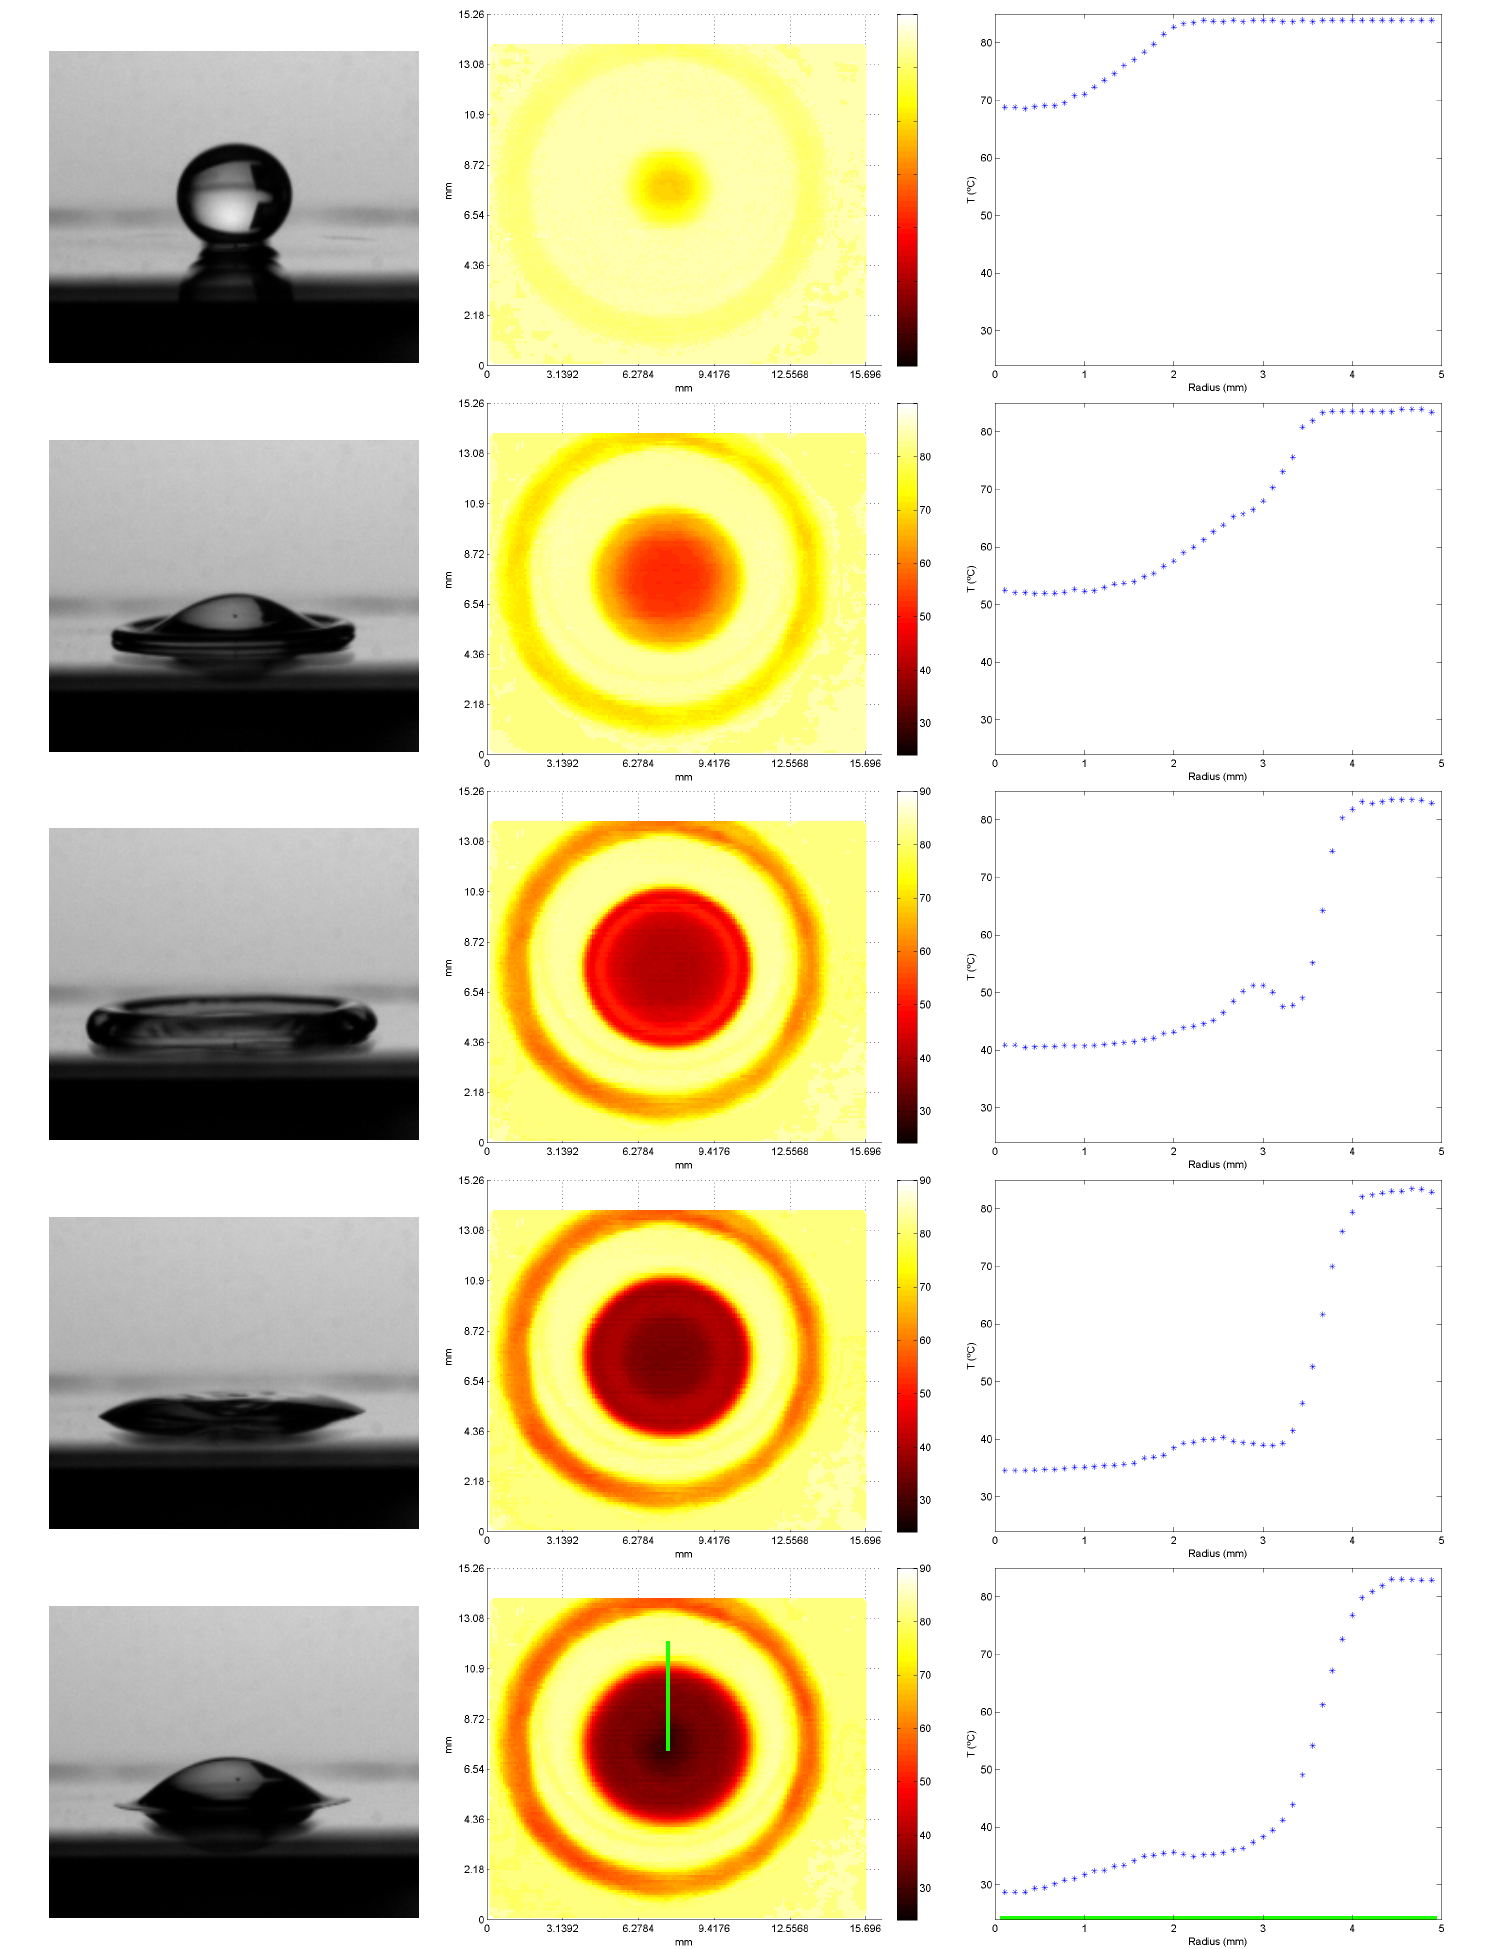
\includegraphics[width=1\linewidth]{Figures/5.Chapter/IRvsHR.png}
\caption{Comparison between High Speed camera images and Infra Red images for 0.8m/s and 80ºC at 0, 2, 6, 12 and 22 ms after the first contact on a hydrophilic surface}
\label{fig:irvshr}
\end{figure}

\par One of the main objectives of this work is to use the high-speed camera simultaneously with the IR Camera to compare physical phenomena with thermal phenomena. The results were put together in Figure \ref{fig:irvshr}. In this figure it is possible to see some of the stages of a droplet impact. Analyzing the images, it's observable the physical phenomena that have an impact on heat transfer. During the spreading, the lamella's rim is visible in the temperature maps, as introduced in Section \ref{sec:heat}, starts forming in the second millisecond. When the edge reaches maximum diameter it reverses direction and starts the recoiling phase, shown in the 12 ms images. The thickness of the water layer is smaller right before the lamella's edge. In this area there is less heat removal. So, as expected, one can see a ring of higher temperatures, and a slope in the plot. After the recoiling phase the droplet starts to stabilize, and due to it's hemispherical shape the heat flux is higher at the center, so the temperature is lower in the center. Although here there is no rim in the lamella by this phase, one can clearly see the lighter ring on the IR Image. This is the cause of thermal inertia.

\par Another type of results can be obtained for the collected data and these are the heat flux and cooling effectiveness. Starting with the heat flux, an example of the obtained graphic can be seen in Figure \ref{fig:fluex}. Looking at the heat flux, one can see the expected phenomena, described in the literature \cite{pasandideh2001cooling}. There are only some comparable results between Figure \ref{fig:fluxo} and the collected results, as the timestep of the simulation is much smaller. The contact edge heat flux peak couldn't be captured in the initial timesteps, but is clear in the posterior frames. This contact edge peak is a reflection of cold water being pushed to the edge of the lamella as the droplet spreads. In the center the spatial gradient is ignored because of the problem's axisymmetry. The highest peaks for the initial times aren't captured by the IR Camera, but the flux drop before the peak, in Figure \ref{fig:fluxo}, is visible in the 1ms and 2ms frame. The spatial dispersion of the flux in early frames is clear in the experimental results. This may be caused by thermal inertia and heat diffusion along the foil. This may also be the cause for the innexistence of a peak in the early frames. In the last frame, which, according to Figure \ref{fig:diameter}, is already during the receding phase, the heat flux is negative after the droplet edge. This is caused by the area being no longer wetted and is now heating again. Also the heat flux drop before the contact angle peak is an indicative of the presence of the lamella's rim in that area. Also the heat flux is very small compared to other timesteps due to the droplet temperature raise.\\


\begin{figure}[h!]
\centering
\begin{tikzpicture}
\begin{axis}[
	title = {2 m/s || 100 ºC || $T_{amb}=24$},
    tick label style={font=\scriptsize},
    legend style={font=\scriptsize,/tikz/column 2/.style={column sep=5pt},},
    %legend columns=2,
    legend cell align=left,
	legend pos =north east,
    grid=major, % Display a grid
    grid style={dashed,gray!30}, % Set the style
    xlabel={Droplet Radius (mm)},
    ylabel={$q''(W/m^2)$}, 
    %ymin = 15, ymax = 125,
    %ytick={20,40,...,120},
    %yticklabels={300,325,350,375,400,425,450,475,500,525},
    xmin = 0, xmax = 7.5,
    %ytick={0,1600,...,11200},
    %yticklabel style={
    %    /pgf/number format/fixed,
    %    /pgf/number format/precision=5},
	%scaled y ticks=false,
    width=0.9\textwidth, 
    height=9cm,
    cycle list name= color
    ]
\addplot+[dashed]
coordinates {(	0	,	1777670.079	)
(	0.11	,	1792323.198	)
(	0.22	,	1797061.305	)
(	0.33	,	1789569.185	)
(	0.44	,	1789015.722	)
(	0.55	,	1803622.248	)
(	0.65	,	1836659.277	)
(	0.76	,	1868745.749	)
(	0.87	,	1890207.195	)
(	0.98	,	1872770.186	)
(	1.09	,	1858985.806	)
(	1.2	,	1866796.219	)
(	1.31	,	1886797.855	)
(	1.42	,	1871035.553	)
(	1.53	,	1818458.79	)
(	1.64	,	1738103.547	)
(	1.75	,	1650076.058	)
(	1.86	,	1578011.828	)
(	1.96	,	1521786.363	)
(	2.07	,	1463673.962	)
(	2.18	,	1356450.868	)
(	2.29	,	1234687.338	)
(	2.4	,	1131209.047	)
(	2.51	,	1051299.604	)
(	2.62	,	964361.1129	)
(	2.73	,	890905.7486	)
(	2.84	,	820486.8888	)
(	2.95	,	757411.9607	)
(	3.06	,	700437.3131	)
(	3.17	,	644241.2043	)
(	3.27	,	584413.7383	)
(	3.38	,	492724.449	)
(	3.49	,	387796.4609	)
(	3.6	,	264656.6861	)
(	3.71	,	158383.9646	)
(	3.82	,	68032.80929	)
(	3.93	,	23332.98041	)
(	4.04	,	8824.872215	)
(	4.15	,	2783.827432	)
(	4.26	,	-2946.812742	)
(	4.37	,	1783.017459	)
(	4.48	,	17428.61908	)
(	4.59	,	27766.9984	)
(	4.7	,	25929.14618	)
(	4.81	,	8913.264039	)
(	4.92	,	-461.1725983	)
(	5.03	,	-3885.427042	)
(	5.14	,	10510.44467	)
(	5.25	,	33569.04446	)
(	5.36	,	24609.65614	)
(	5.47	,	6504.078318	)
(	5.58	,	14471.4661	)
(	5.69	,	35286.16241	)
(	5.8	,	22937.69419	)
(	5.91	,	16717.33533	)
(	6.02	,	19095.65158	)
(	6.13	,	26500.66468	)
(	6.24	,	17516.80911	)
(	6.35	,	32445.82136	)
(	6.46	,	62028.02361	)
};
\addlegendentry{1 ms}

\addplot+[dashed]
coordinates {(	0	,	994416.6114	)
(	0.11	,	977868.5786	)
(	0.22	,	972484.0558	)
(	0.33	,	979964.5653	)
(	0.44	,	1009224.339	)
(	0.55	,	1024051.643	)
(	0.65	,	1035507.694	)
(	0.76	,	1018875.215	)
(	0.87	,	1033036.687	)
(	0.98	,	1047901.012	)
(	1.09	,	1067866.738	)
(	1.2	,	1066642.971	)
(	1.31	,	1070797.553	)
(	1.42	,	1086486.604	)
(	1.53	,	1127965.656	)
(	1.64	,	1185262.461	)
(	1.75	,	1237552.837	)
(	1.86	,	1287648.943	)
(	1.96	,	1296848.547	)
(	2.07	,	1326923.578	)
(	2.18	,	1351476.86	)
(	2.29	,	1380984.107	)
(	2.4	,	1382032.351	)
(	2.51	,	1399104.992	)
(	2.62	,	1386742.3	)
(	2.73	,	1361384.005	)
(	2.84	,	1332532.503	)
(	2.95	,	1291867.248	)
(	3.06	,	1275120.227	)
(	3.17	,	1264695.521	)
(	3.27	,	1297790.475	)
(	3.38	,	1310759.548	)
(	3.49	,	1357356.743	)
(	3.6	,	1401558.802	)
(	3.71	,	1462662.38	)
(	3.82	,	1466663.884	)
(	3.93	,	1439063.016	)
(	4.04	,	1380067.453	)
(	4.15	,	1304513.447	)
(	4.26	,	1213606.763	)
(	4.37	,	1097774.749	)
(	4.48	,	963623.8334	)
(	4.59	,	732954.8917	)
(	4.7	,	396736.0879	)
(	4.81	,	104345.5448	)
(	4.92	,	-870.3142338	)
(	5.03	,	12710.59066	)
(	5.14	,	5768.502396	)
(	5.25	,	29015.00339	)
(	5.36	,	40107.34728	)
(	5.47	,	29735.44666	)
(	5.58	,	-3364.906372	)
(	5.69	,	13370.9096	)
(	5.8	,	17872.4023	)
(	5.91	,	22126.82747	)
(	6.02	,	-8408.393299	)
(	6.13	,	10462.99961	)
(	6.24	,	25645.7798	)
(	6.35	,	34831.77943	)
(	6.46	,	42268.81389	)
};
\addlegendentry{2 ms}

\addplot+[dashed]
coordinates {(	0	,	603064.3463	)
(	0.11	,	624155.5002	)
(	0.22	,	634775.6785	)
(	0.33	,	635817.91	)
(	0.44	,	629201.713	)
(	0.55	,	612380.4361	)
(	0.65	,	611141.2904	)
(	0.76	,	614518.6137	)
(	0.87	,	639263.8912	)
(	0.98	,	643016.4578	)
(	1.09	,	638055.9843	)
(	1.2	,	625042.0919	)
(	1.31	,	637498.6336	)
(	1.42	,	655804.2419	)
(	1.53	,	678635.2239	)
(	1.64	,	678356.8117	)
(	1.75	,	663833.9141	)
(	1.86	,	692052.9325	)
(	1.96	,	726551.8769	)
(	2.07	,	754922.872	)
(	2.18	,	760996.0219	)
(	2.29	,	792131.7898	)
(	2.4	,	814447.3634	)
(	2.51	,	824594.7305	)
(	2.62	,	839016.7419	)
(	2.73	,	862401.9629	)
(	2.84	,	889489.0656	)
(	2.95	,	879038.4351	)
(	3.06	,	882606.5422	)
(	3.17	,	871410.2777	)
(	3.27	,	907012.3569	)
(	3.38	,	906458.1065	)
(	3.49	,	918781.3111	)
(	3.6	,	900146.4512	)
(	3.71	,	915250.0093	)
(	3.82	,	916395.6412	)
(	3.93	,	925676.8402	)
(	4.04	,	923134.3643	)
(	4.15	,	920740.267	)
(	4.26	,	945088.9664	)
(	4.37	,	964036.3589	)
(	4.48	,	1009509.317	)
(	4.59	,	1187293.301	)
(	4.7	,	1402253.392	)
(	4.81	,	1489327.946	)
(	4.92	,	1412503.751	)
(	5.03	,	1190138.551	)
(	5.14	,	749668.3149	)
(	5.25	,	318611.3815	)
(	5.36	,	73410.27007	)
(	5.47	,	3362.420853	)
(	5.58	,	-11355.62687	)
(	5.69	,	18396.49532	)
(	5.8	,	18544.54954	)
(	5.91	,	30972.18988	)
(	6.02	,	37995.05356	)
(	6.13	,	43685.05832	)
(	6.24	,	1163.995451	)
(	6.35	,	2341.005655	)
(	6.46	,	27134.28976	)
};
\addlegendentry{3 ms}

\addplot+[dashed]
coordinates {(	0	,	320780.4113	)
(	0.11	,	322027.6391	)
(	0.22	,	315052.8158	)
(	0.33	,	301152.4488	)
(	0.44	,	282122.0079	)
(	0.55	,	265290.6522	)
(	0.65	,	266169.1026	)
(	0.76	,	275245.6342	)
(	0.87	,	295179.1577	)
(	0.98	,	284971.8709	)
(	1.09	,	266662.5513	)
(	1.2	,	257241.0431	)
(	1.31	,	261797.6522	)
(	1.42	,	269508.7085	)
(	1.53	,	294921.2306	)
(	1.64	,	311712.3099	)
(	1.75	,	303673.5151	)
(	1.86	,	303177.924	)
(	1.96	,	302007.3942	)
(	2.07	,	310736.0391	)
(	2.18	,	305672.0705	)
(	2.29	,	305465.7618	)
(	2.4	,	333973.8913	)
(	2.51	,	356521.1072	)
(	2.62	,	357853.7584	)
(	2.73	,	361005.0809	)
(	2.84	,	391630.3511	)
(	2.95	,	397969.6682	)
(	3.06	,	400059.2988	)
(	3.17	,	382182.46	)
(	3.27	,	389759.2535	)
(	3.38	,	387407.374	)
(	3.49	,	399341.1009	)
(	3.6	,	393431.7364	)
(	3.71	,	399282.5975	)
(	3.82	,	401598.2573	)
(	3.93	,	424168.3651	)
(	4.04	,	452934.3216	)
(	4.15	,	455794.4431	)
(	4.26	,	443446.1916	)
(	4.37	,	441736.4147	)
(	4.48	,	436149.3999	)
(	4.59	,	435533.1267	)
(	4.7	,	444943.1989	)
(	4.81	,	478610.1544	)
(	4.92	,	565836.1945	)
(	5.03	,	739130.7952	)
(	5.14	,	992480.6647	)
(	5.25	,	1085579.768	)
(	5.36	,	662871.2143	)
(	5.47	,	75691.55777	)
(	5.58	,	-128074.1393	)
(	5.69	,	-12539.71762	)
(	5.8	,	8467.379924	)
(	5.91	,	-25147.30309	)
(	6.02	,	-7974.952403	)
(	6.13	,	8905.195037	)
(	6.24	,	-6670.026193	)
(	6.35	,	-2233.284817	)
(	6.46	,	11121.67094	)
};
\addlegendentry{5 ms}

\addplot+[dashed]
coordinates {(	0	,	122436.4468	)
(	0.11	,	124830.3464	)
(	0.22	,	116426.4897	)
(	0.33	,	87430.23932	)
(	0.44	,	91210.56975	)
(	0.55	,	116888.1093	)
(	0.65	,	130871.0749	)
(	0.76	,	117329.6391	)
(	0.87	,	118667.2846	)
(	0.98	,	116254.7647	)
(	1.09	,	117938.4013	)
(	1.2	,	119205.8729	)
(	1.31	,	117021.3663	)
(	1.42	,	113510.981	)
(	1.53	,	118135.8538	)
(	1.64	,	120155.1482	)
(	1.75	,	116294.9573	)
(	1.86	,	115750.9814	)
(	1.96	,	118657.9074	)
(	2.07	,	112225.837	)
(	2.18	,	71197.11591	)
(	2.29	,	69892.47851	)
(	2.4	,	80237.98858	)
(	2.51	,	97774.42538	)
(	2.62	,	89674.07039	)
(	2.73	,	121155.1818	)
(	2.84	,	107048.0623	)
(	2.95	,	86840.12141	)
(	3.06	,	79603.94473	)
(	3.17	,	66954.23935	)
(	3.27	,	57932.05869	)
(	3.38	,	58726.62553	)
(	3.49	,	62495.15826	)
(	3.6	,	46288.4161	)
(	3.71	,	66479.28359	)
(	3.82	,	90384.50841	)
(	3.93	,	106459.0508	)
(	4.04	,	111952.8542	)
(	4.15	,	115616.0474	)
(	4.26	,	100128.1898	)
(	4.37	,	125135.9039	)
(	4.48	,	137405.2507	)
(	4.59	,	140877.074	)
(	4.7	,	95743.31096	)
(	4.81	,	49746.23833	)
(	4.92	,	4298.077883	)
(	5.03	,	18092.17592	)
(	5.14	,	59670.36515	)
(	5.25	,	128003.0867	)
(	5.36	,	134698.0039	)
(	5.47	,	37592.31552	)
(	5.58	,	-82901.73639	)
(	5.69	,	-51120.38828	)
(	5.8	,	686.5143774	)
(	5.91	,	-2665.658593	)
(	6.02	,	-44802.83426	)
(	6.13	,	-3415.328045	)
(	6.24	,	-3100.137655	)
(	6.35	,	3716.529412	)
(	6.46	,	7551.782406	)
};
\addlegendentry{10 ms}
\end{axis}
\end{tikzpicture}
\caption{Heat Flux along the radius of a water droplet, $u_i=2m/s$, Surface temperature=100ºC}
\label{fig:fluex}
\end{figure}

\par Observing the cooling efficiency graphic in Figure \ref{fig:coolex}, a comparison with \cite{pasandideh2001cooling} can be made. Using this graphic as a reference a very similar evolution with time can be seen. The adimensional parameter $t^*$ is used to consider the impact velocity in a comparison. The evolution stagnates as the droplet's temperature increases and the foil temperature decreases. The cooling effectiveness is higher in the numerical results. This may be the cause of a different initial flux or foil size. It can also be the cause of the ideal conditions assumed in the numerical simulation.\\

\begin{figure}[h!]
\centering
\subfigure[Detail view]{\begin{tikzpicture}
\begin{axis}[
	title = {2 m/s || 120 ºC || $T_{amb}=24$},
    tick label style={font=\scriptsize},
    legend style={font=\scriptsize,/tikz/column 2/.style={column sep=5pt},},
    %legend columns=2,
    legend cell align=left,
	legend pos =north west,
    grid=major, % Display a grid
    grid style={dashed,gray!30}, % Set the style
    xlabel={$t^*=t$\Large{$\frac{u_i}{D_0}$}},
    ylabel={$\varepsilon$}, 
    ymin = 0, ymax = 0.2,
    ytick={0,0.04,0.08,0.12,0.16,0.2},
    yticklabels={0,0.04,0.08,0.12,0.16,0.2},
    xmin = 0, xmax = 5,
    %ytick={0,1600,...,11200},
    %yticklabel style={
    %    /pgf/number format/fixed,
    %    /pgf/number format/precision=5},
	%scaled y ticks=false,
    width=0.5\textwidth, 
    height=7cm,
    cycle list name= color
    ]
\addplot+[dashed]
coordinates {(	0	,	0	)
(	0.740740741	,	0.006183436	)
(	1.481481481	,	0.027132397	)
(	2.222222222	,	0.055947222	)
(	2.962962963	,	0.081489615	)
(	3.703703704	,	0.101288971	)
(	4.444444444	,	0.115230298	)
(	5.185185185	,	0.124822088	)
(	5.925925926	,	0.131242371	)
(	6.666666667	,	0.135432275	)
(	7.407407407	,	0.138496222	)
(	8.148148148	,	0.140580511	)
(	8.888888889	,	0.14177022	)
(	9.62962963	,	0.14257969	)
(	10.37037037	,	0.143075045	)
(	11.11111111	,	0.143348662	)
(	11.85185185	,	0.143623278	)
(	12.59259259	,	0.143854086	)
(	13.33333333	,	0.143895141	)
(	14.07407407	,	0.143929706	)
(	14.81481481	,	0.144092568	)
(	15.55555556	,	0.144183357	)
(	16.2962963	,	0.144236892	)
(	17.03703704	,	0.144266432	)
(	17.77777778	,	0.144186044	)
(	18.51851852	,	0.144202142	)
(	19.25925926	,	0.144378417	)
(	20	,	0.144427272	)
(	20.74074074	,	0.144534209	)
(	21.48148148	,	0.14483881	)
(	22.22222222	,	0.145008105	)
(	22.96296296	,	0.145183721	)
(	23.7037037	,	0.145324486	)
(	24.44444444	,	0.145476178	)
(	25.18518519	,	0.145726953	)
(	25.92592593	,	0.145933468	)
(	26.66666667	,	0.146100459	)
(	27.40740741	,	0.146233525	)
(	28.14814815	,	0.146439453	)
(	28.88888889	,	0.14653441	)
(	29.62962963	,	0.146576075	)
(	30.37037037	,	0.146660443	)
(	31.11111111	,	0.146754592	)
(	31.85185185	,	0.146974795	)
(	32.59259259	,	0.147098626	)
(	33.33333333	,	0.147180226	)
(	34.07407407	,	0.147398825	)
(	34.81481481	,	0.14764873	)
(	35.55555556	,	0.147820618	)
(	36.2962963	,	0.147923815	)
(	37.03703704	,	0.148112059	)
(	37.77777778	,	0.148315615	)
(	38.51851852	,	0.148439	)
(	39.25925926	,	0.148571693	)
(	40	,	0.148709699	)
(	40.74074074	,	0.148776587	)
(	41.48148148	,	0.148849014	)
(	42.22222222	,	0.148966825	)
(	42.96296296	,	0.149264835	)
(	43.7037037	,	0	)
};
\addlegendentry{Experimental results}
\addplot[
    domain=0:5, 
    samples=20,
    color=red,
]{-1.6221*10^(-5)*x^6 + 5.5731*10^(-5)*x^5 + 1.4888*10^(-3)*x^4 - 1.2942*10^(-2)*x^3 + 3.7275*10^(-2)*x^2 + 3.8779*10^(-3)*x + 6.0277*10^(-4)};
\addlegendentry{M.Pasadideh-Fard \textit{et. al} (num)}
\end{axis}
\end{tikzpicture}}
\subfigure[Full view]{\begin{tikzpicture}
\begin{axis}[
	title = {2 m/s || 120 ºC || $T_{amb}=24$},
    tick label style={font=\scriptsize},
    legend style={font=\scriptsize,/tikz/column 2/.style={column sep=5pt},},
    %legend columns=2,
    legend cell align=left,
	legend pos =north east,
    grid=major, % Display a grid
    grid style={dashed,gray!30}, % Set the style
    xlabel={$t^*=t$\Large{$\frac{u_i}{D_0}$}},
    ylabel={$\varepsilon$}, 
    ymin = 0, ymax = 0.16,
    ytick={0,0.02,0.04,0.06,0.08,0.1,0.12,0.14,0.16},
    yticklabels={0,0.02,0.04,0.06,0.08,0.1,0.12,0.14,0.16},
    xmin = 0, xmax = 43,
    %ytick={0,1600,...,11200},
    %yticklabel style={
    %    /pgf/number format/fixed,
    %    /pgf/number format/precision=5},
	%scaled y ticks=false,
    width=0.5\textwidth, 
    height=7cm,
    cycle list name= color
    ]
\addplot+[dashed]
coordinates {(	0	,	0	)
(	0.740740741	,	0.006183436	)
(	1.481481481	,	0.027132397	)
(	2.222222222	,	0.055947222	)
(	2.962962963	,	0.081489615	)
(	3.703703704	,	0.101288971	)
(	4.444444444	,	0.115230298	)
(	5.185185185	,	0.124822088	)
(	5.925925926	,	0.131242371	)
(	6.666666667	,	0.135432275	)
(	7.407407407	,	0.138496222	)
(	8.148148148	,	0.140580511	)
(	8.888888889	,	0.14177022	)
(	9.62962963	,	0.14257969	)
(	10.37037037	,	0.143075045	)
(	11.11111111	,	0.143348662	)
(	11.85185185	,	0.143623278	)
(	12.59259259	,	0.143854086	)
(	13.33333333	,	0.143895141	)
(	14.07407407	,	0.143929706	)
(	14.81481481	,	0.144092568	)
(	15.55555556	,	0.144183357	)
(	16.2962963	,	0.144236892	)
(	17.03703704	,	0.144266432	)
(	17.77777778	,	0.144186044	)
(	18.51851852	,	0.144202142	)
(	19.25925926	,	0.144378417	)
(	20	,	0.144427272	)
(	20.74074074	,	0.144534209	)
(	21.48148148	,	0.14483881	)
(	22.22222222	,	0.145008105	)
(	22.96296296	,	0.145183721	)
(	23.7037037	,	0.145324486	)
(	24.44444444	,	0.145476178	)
(	25.18518519	,	0.145726953	)
(	25.92592593	,	0.145933468	)
(	26.66666667	,	0.146100459	)
(	27.40740741	,	0.146233525	)
(	28.14814815	,	0.146439453	)
(	28.88888889	,	0.14653441	)
(	29.62962963	,	0.146576075	)
(	30.37037037	,	0.146660443	)
(	31.11111111	,	0.146754592	)
(	31.85185185	,	0.146974795	)
(	32.59259259	,	0.147098626	)
(	33.33333333	,	0.147180226	)
(	34.07407407	,	0.147398825	)
(	34.81481481	,	0.14764873	)
(	35.55555556	,	0.147820618	)
(	36.2962963	,	0.147923815	)
(	37.03703704	,	0.148112059	)
(	37.77777778	,	0.148315615	)
(	38.51851852	,	0.148439	)
(	39.25925926	,	0.148571693	)
(	40	,	0.148709699	)
(	40.74074074	,	0.148776587	)
(	41.48148148	,	0.148849014	)
(	42.22222222	,	0.148966825	)
(	42.96296296	,	0.149264835	)
(	43.7037037	,	0	)
};
%\addlegendentry{2 m/s}
\end{axis}
\end{tikzpicture}}
\caption{Cooling effectiveness along $t^*$ for a water droplet impacting on an hydrophilic surface}
\label{fig:coolex}
\end{figure}

\subsection{Influence of the impact velocity}

\par For an hydrophilic surface (the stainless steel foil), results were taken for different impact velocities: 0.8 m/s, 2 m/s at an initial heating of 100ºC. At this temperature, boiling of the lamella is not yet observed. The two impact velocities are compared in Figure \ref{fig:hsspeed} The obvious difference is observed between the droplet spreading at different impact velocities is the spreading diameter, which is directly influenced by the impact velocity. One of the differences is the fingering, that only happens for 2 m/s (at t= 6ms). The height of the lamella is also smaller for this velocity.\\

\begin{figure}[h]
\centering
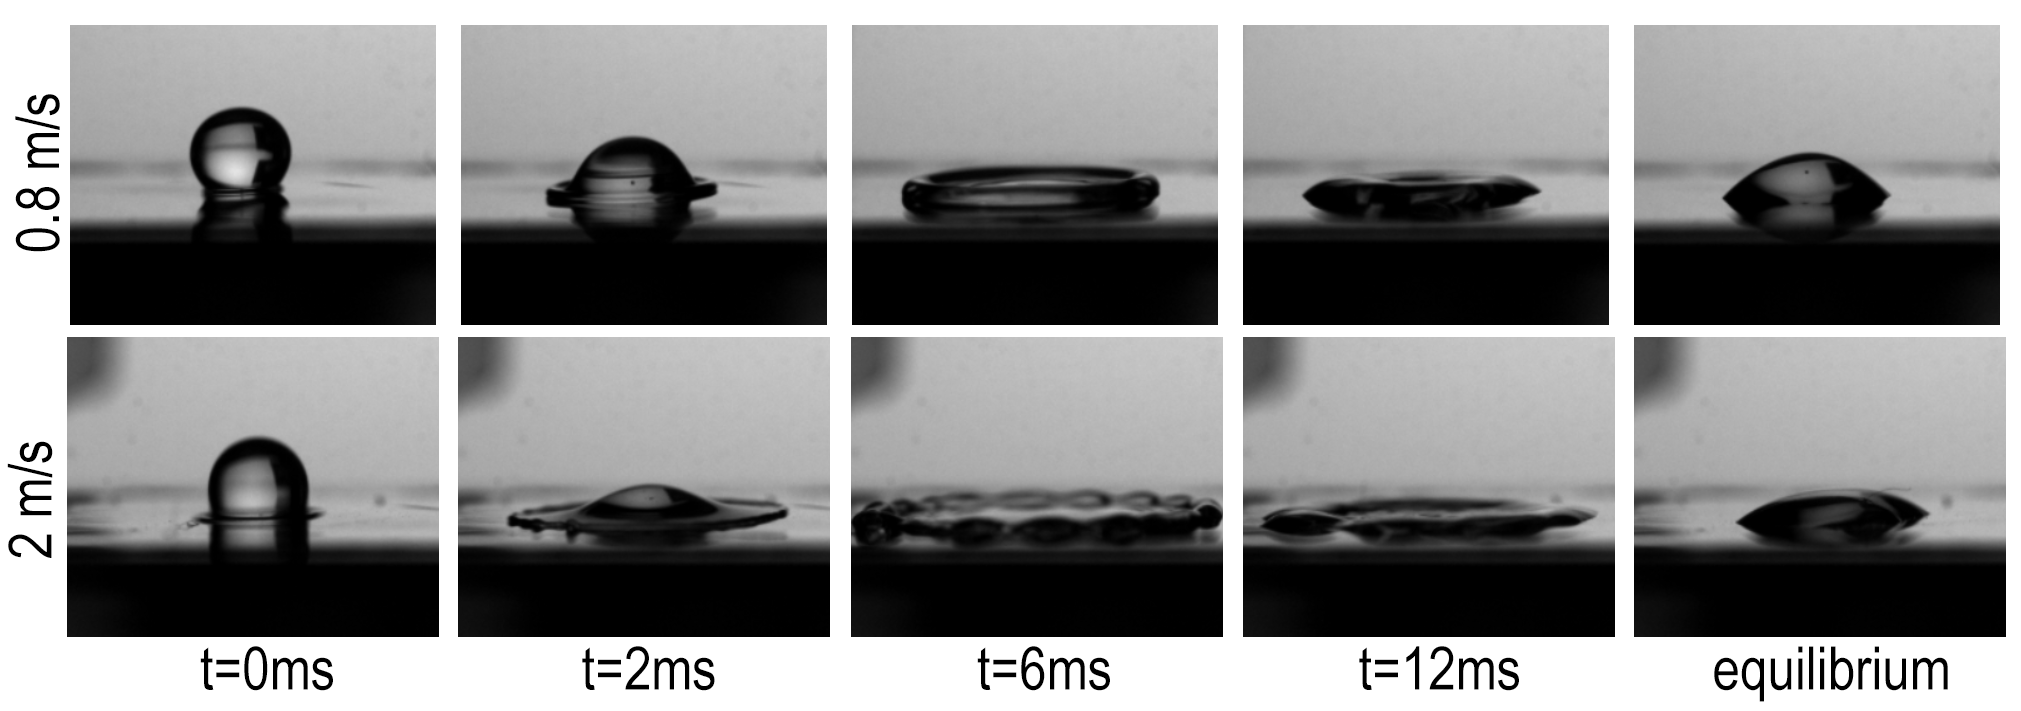
\includegraphics[width=1\linewidth]{Figures/5.Chapter/hsspeed.png}
\caption{Comparison of droplet impact at 0.8m/s and 2m/s. The water droplet impacts the surface at an initial temperature of 100ºC}
\label{fig:hsspeed}
\end{figure}

\par Using the high speed camera it was possible to extract the droplet diameter for each frame, with the help of a code developed previously by Tomás Valente. The comparison between the spreading factor of each velocity can be seen in Figure \ref{fig:diameter}. As expected the spreading factor grows more with a higher impact velocity. In this figure the difference between the maximum diameter time can be compared. In the case of 2 m/s the time in which the maximum diameter occurs is at approximately 4 ms, and in the case of 0.8 m/s occurs at 6 ms. The spreading factor difference in maximum diameter has a relation of approximately 2,5 to 4, which is considerably larger.\\

\begin{figure}[h]
\centering
\begin{tikzpicture}
\begin{axis}[
	title = {Spreading Diameter},
    tick label style={font=\scriptsize},
    legend style={font=\scriptsize,/tikz/column 2/.style={column sep=5pt},},
    %legend columns=2,
    legend cell align=left,
	legend pos =south east,
    grid=major, % Display a grid
    grid style={dashed,gray!30}, % Set the style
    xlabel={Time (s)},
    ylabel={Spreading Factor $\beta$}, 
    ymin = 0, ymax = 4.5,
    ytick={0,0.5,...,4.5},
    %yticklabels={300,325,350,375,400,425,450,475,500,525},
    xmin = 0, xmax = 0.025,
    %ytick={0,1600,...,11200},
    %yticklabel style={
    %    /pgf/number format/fixed,
    %    /pgf/number format/precision=5},
	%scaled y ticks=false,
    width=1\textwidth, height=5cm,
    cycle list name= color
    ]
\addplot+[dashed]
coordinates {(	0	,	0.515151515	)
(	0.000454545	,	1.939393939	)
(	0.000909091	,	2.636363636	)
(	0.001363636	,	3.015151515	)
(	0.001818182	,	3.363636364	)
(	0.002272727	,	3.545454545	)
(	0.002727273	,	3.712121212	)
(	0.003181818	,	3.787878788	)
(	0.003636364	,	3.833333333	)
(	0.004090909	,	3.863636364	)
(	0.004545455	,	3.848484848	)
(	0.005	,	3.818181818	)
(	0.005454545	,	3.818181818	)
(	0.005909091	,	3.833333333	)
(	0.006363636	,	3.772727273	)
(	0.006818182	,	3.757575758	)
(	0.007272727	,	3.772727273	)
(	0.007727273	,	3.681818182	)
(	0.008181818	,	3.696969697	)
(	0.008636364	,	3.621212121	)
(	0.009090909	,	3.621212121	)
(	0.01	,	3.53030303	)
(	0.010909091	,	3.454545455	)
(	0.011818182	,	3.393939394	)
(	0.012727273	,	3.318181818	)
(	0.013636364	,	3.242424242	)
(	0.014545455	,	3.106060606	)
(	0.015454545	,	3.090909091	)
(	0.019090909	,	2.818181818	)
(	0.022727273	,	2.636363636	)
};
\addlegendentry{2 m/s}

\addplot+[dashed]
coordinates {(	0	,	0.166303558	)
(	0.000454545	,	0.680332739	)
(	0.000909091	,	1.179243415	)
(	0.001363636	,	1.602561563	)
(	0.001818182	,	1.889813164	)
(	0.002272727	,	2.131709249	)
(	0.002727273	,	2.298012808	)
(	0.003181818	,	2.403842345	)
(	0.003636364	,	2.479434872	)
(	0.004090909	,	2.539908893	)
(	0.004545455	,	2.570145903	)
(	0.005	,	2.585264409	)
(	0.005454545	,	2.585264409	)
(	0.005909091	,	2.585264409	)
(	0.006363636	,	2.585264409	)
(	0.006818182	,	2.570145903	)
(	0.007272727	,	2.570145903	)
(	0.007727273	,	2.555027398	)
(	0.008181818	,	2.539908893	)
(	0.008636364	,	2.524790388	)
(	0.009090909	,	2.509671882	)
(	0.009545455	,	2.494553377	)
(	0.01	,	2.479434872	)
(	0.010454545	,	2.449197861	)
(	0.010909091	,	2.434079356	)
(	0.011363636	,	2.403842345	)
(	0.011818182	,	2.38872384	)
(	0.012272727	,	2.373605334	)
(	0.012727273	,	2.343368324	)
(	0.013181818	,	2.343368324	)
(	0.013636364	,	2.313131313	)
(	0.014090909	,	2.282894303	)
(	0.014545455	,	2.282894303	)
(	0.015	,	2.252657292	)
(	0.015454545	,	2.237538787	)
(	0.015909091	,	2.222420281	)
(	0.016363636	,	2.207301776	)
(	0.016818182	,	2.177064765	)
(	0.017272727	,	2.16194626	)
(	0.017727273	,	2.16194626	)
(	0.018181818	,	2.146827755	)
(	0.018636364	,	2.131709249	)
(	0.019090909	,	2.131709249	)
(	0.019545455	,	2.116590744	)
(	0.02	,	2.101472239	)
(	0.020454545	,	2.101472239	)
(	0.020909091	,	2.071235228	)
(	0.021363636	,	2.071235228	)
(	0.021818182	,	2.056116723	)
(	0.022272727	,	2.040998217	)
(	0.022727273	,	2.025879712	)
};
\addlegendentry{0.8 m/s}

\end{axis}
\end{tikzpicture}
\caption{Comparison between the spreading factor of each velocity}
\label{fig:diameter}
\end{figure}
\begin{figure}[h!]
\centering
\begin{tikzpicture}
\begin{axis}[
	%title = {107 ºC || $T_{amb}=24$},
    tick label style={font=\scriptsize},
    legend style={font=\scriptsize,/tikz/column 2/.style={column sep=5pt},},
    %legend columns=2,
    legend cell align=left,
	legend pos =south east,
    grid=major, % Display a grid
    grid style={dashed,gray!30}, % Set the style
    xlabel={Droplet Radius (mm)},
    ylabel={T (ºC)}, 
    ymin = 55, ymax = 113,
    ytick={60,70,...,100,110},
    %yticklabels={300,325,350,375,400,425,450,475,500,525},
    xmin = 0, xmax = 7,
    %ytick={0,1600,...,11200},
    %yticklabel style={
    %    /pgf/number format/fixed,
    %    /pgf/number format/precision=5},
	%scaled y ticks=false,
    width=0.5\textwidth, height=6.5cm,
    cycle list name= color
    ]
\addplot+[dashed]
coordinates {(	0	,	65.76	)
(	0.12	,	65.9	)
(	0.23	,	65.85	)
(	0.35	,	66.09	)
(	0.46	,	66.07	)
(	0.58	,	66.22	)
(	0.69	,	66.79	)
(	0.81	,	67.14	)
(	0.92	,	67.57	)
(	1.04	,	68.07	)
(	1.16	,	68.69	)
(	1.27	,	69.25	)
(	1.39	,	70.14	)
(	1.5	,	71.11	)
(	1.62	,	72.38	)
(	1.73	,	73.98	)
(	1.85	,	75.64	)
(	1.97	,	77.5	)
(	2.08	,	79.6	)
(	2.2	,	81.25	)
(	2.31	,	82.46	)
(	2.43	,	84	)
(	2.54	,	85.63	)
(	2.66	,	87.47	)
(	2.77	,	89.31	)
(	2.89	,	91.96	)
(	3.01	,	94.76	)
(	3.12	,	97.56	)
(	3.24	,	99.83	)
(	3.35	,	101.74	)
(	3.47	,	102.78	)
(	3.58	,	103.09	)
(	3.7	,	103.17	)
(	3.81	,	103.25	)
(	3.93	,	103.13	)
(	4.05	,	103.23	)
(	4.16	,	103.22	)
(	4.28	,	103.31	)
(	4.39	,	103.17	)
(	4.51	,	103.02	)
(	4.62	,	102.99	)
};
\addlegendentry{0.8 m/s - 3 ms}

\addplot+[dashed]
coordinates {(	0	,	64.76	)
(	0.12	,	64.97	)
(	0.23	,	64.61	)
(	0.35	,	64.44	)
(	0.46	,	64.13	)
(	0.58	,	64.08	)
(	0.69	,	64.09	)
(	0.81	,	63.56	)
(	0.92	,	63.26	)
(	1.04	,	63.34	)
(	1.16	,	63.22	)
(	1.27	,	63.12	)
(	1.39	,	63.12	)
(	1.5	,	62.93	)
(	1.62	,	63.29	)
(	1.73	,	63.7	)
(	1.85	,	63.88	)
(	1.97	,	64.17	)
(	2.08	,	64.58	)
(	2.2	,	65.21	)
(	2.31	,	65.97	)
(	2.43	,	66.51	)
(	2.54	,	67.27	)
(	2.66	,	68.47	)
(	2.77	,	69.17	)
(	2.89	,	70.41	)
(	3.01	,	71.01	)
(	3.12	,	72.19	)
(	3.24	,	73.14	)
(	3.35	,	73.85	)
(	3.47	,	74.52	)
(	3.58	,	75.4	)
(	3.7	,	76.25	)
(	3.81	,	77.3	)
(	3.93	,	78.35	)
(	4.05	,	79.18	)
(	4.16	,	80.08	)
(	4.28	,	81.21	)
(	4.39	,	82.8	)
(	4.51	,	84	)
(	4.62	,	85.5	)
(	4.74	,	87.06	)
(	4.85	,	89.03	)
(	4.97	,	90.91	)
(	5.09	,	93.49	)
(	5.2	,	96.19	)
(	5.32	,	100.05	)
(	5.43	,	103.28	)
(	5.55	,	105.25	)
(	5.66	,	106.11	)
(	5.78	,	106.44	)
(	5.9	,	106.29	)
(	6.01	,	106.37	)
(	6.13	,	106.42	)
(	6.24	,	106	)
(	6.36	,	105.96	)
(	6.47	,	105.78	)
(	6.59	,	105.59	)
};
\addlegendentry{2 m/s - 3 ms}

\end{axis}
\end{tikzpicture}
\begin{tikzpicture}
\begin{axis}[
	%title = {107 ºC || $T_{amb}=24$},
    tick label style={font=\scriptsize},
    legend style={font=\scriptsize,/tikz/column 2/.style={column sep=5pt},},
    %legend columns=2,
    legend cell align=left,
	legend pos =north west,
    grid=major, % Display a grid
    grid style={dashed,gray!30}, % Set the style
    xlabel={Droplet Radius (mm)},
    ylabel={T (ºC)}, 
    ymin = 35, ymax = 113,
    ytick={30,40,...,100,110},
    %yticklabels={300,325,350,375,400,425,450,475,500,525},
    xmin = 0, xmax = 7,
    %ytick={0,1600,...,11200},
    %yticklabel style={
    %    /pgf/number format/fixed,
    %    /pgf/number format/precision=5},
	%scaled y ticks=false,
    width=0.5\textwidth, height=6.5cm,
    cycle list name= color
    ]
\addplot+[dashed]
coordinates {(	0	,	40.31	)
(	0.12	,	40.55	)
(	0.23	,	40.46	)
(	0.35	,	40.67	)
(	0.46	,	40.82	)
(	0.58	,	40.91	)
(	0.69	,	41.1	)
(	0.81	,	41.36	)
(	0.92	,	41.52	)
(	1.04	,	41.6	)
(	1.16	,	41.71	)
(	1.27	,	42.12	)
(	1.39	,	42.45	)
(	1.5	,	42.66	)
(	1.62	,	43.31	)
(	1.73	,	43.95	)
(	1.85	,	45.07	)
(	1.97	,	45.77	)
(	2.08	,	46.81	)
(	2.2	,	47.54	)
(	2.31	,	48.29	)
(	2.43	,	49.09	)
(	2.54	,	49.17	)
(	2.66	,	49.05	)
(	2.77	,	48.75	)
(	2.89	,	48.29	)
(	3.01	,	48.6	)
(	3.12	,	49.5	)
(	3.24	,	51.61	)
(	3.35	,	56.13	)
(	3.47	,	61.63	)
(	3.58	,	68.59	)
(	3.7	,	76.42	)
(	3.81	,	84.29	)
(	3.93	,	91.67	)
(	4.05	,	96.84	)
(	4.16	,	100.05	)
(	4.28	,	101.53	)
(	4.39	,	102.28	)
(	4.51	,	102.08	)
(	4.62	,	101.62	)
};
\addlegendentry{0.8 m/s - 13 ms}

\addplot+[dashed]
coordinates {(	0	,	41.51	)
(	0.12	,	41.44	)
(	0.23	,	41.31	)
(	0.35	,	41.14	)
(	0.46	,	40.77	)
(	0.58	,	40.61	)
(	0.69	,	40.39	)
(	0.81	,	40.57	)
(	0.92	,	40.22	)
(	1.04	,	40.24	)
(	1.16	,	40.11	)
(	1.27	,	40.11	)
(	1.39	,	40.05	)
(	1.5	,	39.87	)
(	1.62	,	39.81	)
(	1.73	,	39.79	)
(	1.85	,	39.95	)
(	1.97	,	39.91	)
(	2.08	,	40.28	)
(	2.2	,	40.34	)
(	2.31	,	40.64	)
(	2.43	,	40.65	)
(	2.54	,	41.02	)
(	2.66	,	41.57	)
(	2.77	,	41.97	)
(	2.89	,	42.46	)
(	3.01	,	43.23	)
(	3.12	,	43.95	)
(	3.24	,	44.59	)
(	3.35	,	45.3	)
(	3.47	,	46.08	)
(	3.58	,	46.71	)
(	3.7	,	47.43	)
(	3.81	,	47.91	)
(	3.93	,	48.5	)
(	4.05	,	49.05	)
(	4.16	,	49.05	)
(	4.28	,	49.21	)
(	4.39	,	49.27	)
(	4.51	,	49.33	)
(	4.62	,	49.37	)
(	4.74	,	49.62	)
(	4.85	,	49.94	)
(	4.97	,	50.54	)
(	5.09	,	52.22	)
(	5.2	,	54.01	)
(	5.32	,	57.83	)
(	5.43	,	64.46	)
(	5.55	,	73.26	)
(	5.66	,	82.58	)
(	5.78	,	91.23	)
(	5.9	,	97.63	)
(	6.01	,	101.44	)
(	6.13	,	103.55	)
(	6.24	,	104.15	)
(	6.36	,	104.67	)
(	6.47	,	104.97	)
(	6.59	,	104.65	)
};
\addlegendentry{2 m/s - 13 ms}
\end{axis}
\end{tikzpicture}
\begin{tikzpicture}
\begin{axis}[
	%
    tick label style={font=\scriptsize},
    legend style={font=\scriptsize,/tikz/column 2/.style={column sep=5pt},},
    %legend columns=2,
    legend cell align=left,
	legend pos =north west,
    grid=major, % Display a grid
    grid style={dashed,gray!30}, % Set the style
    xlabel={Droplet Radius (mm)},
    ylabel={T (ºC)}, 
    ymin = 30, ymax = 113,
    ytick={30,40,...,100,110},
    %yticklabels={300,325,350,375,400,425,450,475,500,525},
    xmin = 0, xmax = 7,
    %ytick={0,1600,...,11200},
    %yticklabel style={
    %    /pgf/number format/fixed,
    %    /pgf/number format/precision=5},
	%scaled y ticks=false,
    width=0.5\textwidth, height=6.5cm,
    cycle list name= color
    ]
\addplot+[dashed]
coordinates {(	0	,	31.46	)
(	0.12	,	31.32	)
(	0.23	,	31.38	)
(	0.35	,	31.53	)
(	0.46	,	31.66	)
(	0.58	,	32.15	)
(	0.69	,	32.52	)
(	0.81	,	32.8	)
(	0.92	,	33.75	)
(	1.04	,	33.96	)
(	1.16	,	35	)
(	1.27	,	35.59	)
(	1.39	,	36.46	)
(	1.5	,	36.84	)
(	1.62	,	37.3	)
(	1.73	,	38.14	)
(	1.85	,	38.58	)
(	1.97	,	39.1	)
(	2.08	,	39.81	)
(	2.2	,	40.56	)
(	2.31	,	41.33	)
(	2.43	,	42.55	)
(	2.54	,	43.29	)
(	2.66	,	45.03	)
(	2.77	,	46.72	)
(	2.89	,	49.02	)
(	3.01	,	51.27	)
(	3.12	,	54.26	)
(	3.24	,	57.42	)
(	3.35	,	61.69	)
(	3.47	,	66.25	)
(	3.58	,	70.58	)
(	3.7	,	75.28	)
(	3.81	,	79.81	)
(	3.93	,	84.25	)
(	4.05	,	88.44	)
(	4.16	,	91.48	)
(	4.28	,	94.72	)
(	4.39	,	97	)
(	4.51	,	98.21	)
(	4.62	,	99.1	)
};
\addlegendentry{0.8 m/s - 54 ms}

\addplot+[dashed]
coordinates {(	0	,	35.05	)
(	0.12	,	34.63	)
(	0.23	,	34.58	)
(	0.35	,	34.24	)
(	0.46	,	34.48	)
(	0.58	,	34.4	)
(	0.69	,	34.56	)
(	0.81	,	34.42	)
(	0.92	,	34.26	)
(	1.04	,	34.72	)
(	1.16	,	34.6	)
(	1.27	,	35.17	)
(	1.39	,	35.31	)
(	1.5	,	35.71	)
(	1.62	,	35.84	)
(	1.73	,	36.19	)
(	1.85	,	36.73	)
(	1.97	,	37.22	)
(	2.08	,	37.44	)
(	2.2	,	37.85	)
(	2.31	,	38.32	)
(	2.43	,	38.85	)
(	2.54	,	39.73	)
(	2.66	,	40.45	)
(	2.77	,	41.01	)
(	2.89	,	41.65	)
(	3.01	,	42.6	)
(	3.12	,	43.01	)
(	3.24	,	43.82	)
(	3.35	,	44.37	)
(	3.47	,	44.7	)
(	3.58	,	45.48	)
(	3.7	,	45.91	)
(	3.81	,	46.53	)
(	3.93	,	47.14	)
(	4.05	,	47.55	)
(	4.16	,	47.86	)
(	4.28	,	48.81	)
(	4.39	,	49.67	)
(	4.51	,	50.37	)
(	4.62	,	51.56	)
(	4.74	,	52.65	)
(	4.85	,	54.44	)
(	4.97	,	56.31	)
(	5.09	,	58.93	)
(	5.2	,	62.17	)
(	5.32	,	65.89	)
(	5.43	,	70.41	)
(	5.55	,	74.98	)
(	5.66	,	79.66	)
(	5.78	,	84.19	)
(	5.9	,	88.29	)
(	6.01	,	92.34	)
(	6.13	,	95.38	)
(	6.24	,	96.93	)
(	6.36	,	98.86	)
(	6.47	,	101.02	)
(	6.59	,	102.02	)
};
\addlegendentry{2 m/s - 54 ms}

\end{axis}
\end{tikzpicture}
\caption{Average temperature along the radius between the 5 experiments of both velocity values at 100ºC}
\label{fig:speed1}
\end{figure}

\par Lets now take a look at the influence of the velocity in the temperature field. In Figure \ref{fig:speed1}, the average of all experiments made for both velocity values at 100ºC is presented for comparison. The temperature at the center of the droplet is similar during the spreading (3ms and 13 ms). The temperature at the droplet center drops more intensely in the lower velocity. This is justified by the height difference, also noticeable in the last panel of Figure \ref{fig:irvshr}. Looking at the shape of the curves, one can observe their similarity.\\

\par The temperature fields can only give us qualitative information. To quantify cooling and compare both velocities, the heat flux and cooling effectiveness should be considered. Starting with the heat flux, the measurements made for an droplet impacting on a hydrophilic surface at initial temperature of 120ºC were taken as an example. The comparison between different impact velocities is shown in Figure \ref{fig:speedflux}. For both time frames, the contact edge can be easily identified, and the same phenomena are present: the contact edge peak, the peak and drop of the flux caused by the lamella's rim and the heat flux drop in the center due to the trapped gas bubble effect. Overall the flux is higher in the 2 m/s due to the wetted area being larger. The fact that the lamella is thinner in the 2 m/s impact velocity tests, is compensated by the increase in convection heat transfer. As seen before, when reaching equilibrium, the lamella is hotter for the 2 m/s measurements. This is the cause of having a thinner lamella with greater heat flux promoted by convection, which heats the droplet to higher temperatures than in the 0.8 m/s impact velocity case study. This can be also related to the fact that even though the lamella thickness is higher in lower velocities, the heat flux is comparable or even lower, as seen in the figure.\\

\begin{figure}[h!]
\centering
\subfigure[t=2ms]{\begin{tikzpicture}
\begin{axis}[
	%title = {107 ºC || $T_{amb}=24$},
    tick label style={font=\scriptsize},
    legend style={font=\scriptsize,/tikz/column 2/.style={column sep=5pt},},
    %legend columns=2,
    legend cell align=left,
	legend pos =south west,
    grid=major, % Display a grid
    grid style={dashed,gray!30}, % Set the style
    xlabel={Droplet Radius (mm)},
    ylabel={$q''(W/m^2)$}, 
    %ymin = 55, ymax = 113,
    %ytick={60,70,...,100,110},
    %yticklabels={300,325,350,375,400,425,450,475,500,525},
    xmin = 0, xmax = 6,
    %ytick={0,1600,...,11200},
    %yticklabel style={
    %    /pgf/number format/fixed,
    %    /pgf/number format/precision=5},
	%scaled y ticks=false,
    width=0.5\textwidth, height=7cm,
    cycle list name= color
    ]
\addplot+[dashed]
coordinates {(	0	,	1222928.282	)
(	0.11	,	1215849.141	)
(	0.22	,	1213084.596	)
(	0.33	,	1213086.158	)
(	0.44	,	1211400.892	)
(	0.55	,	1235404.245	)
(	0.65	,	1240861.278	)
(	0.76	,	1265052.878	)
(	0.87	,	1242151.87	)
(	0.98	,	1266289.273	)
(	1.09	,	1267085.873	)
(	1.2	,	1313566.011	)
(	1.31	,	1346458.22	)
(	1.42	,	1379273.853	)
(	1.53	,	1395499.139	)
(	1.64	,	1456019.173	)
(	1.75	,	1493810.865	)
(	1.86	,	1473581.581	)
(	1.96	,	1476135.892	)
(	2.07	,	1565916.03	)
(	2.18	,	1634801.538	)
(	2.29	,	1694731.24	)
(	2.4	,	1720340.631	)
(	2.51	,	1744493.418	)
(	2.62	,	1740517.709	)
(	2.73	,	1715786.56	)
(	2.84	,	1685690.399	)
(	2.95	,	1627167.242	)
(	3.06	,	1624506.602	)
(	3.17	,	1624035.892	)
(	3.27	,	1650388.938	)
(	3.38	,	1646634.982	)
(	3.49	,	1705826.365	)
(	3.6	,	1778766.58	)
(	3.71	,	1770709.96	)
(	3.82	,	1677101.721	)
(	3.93	,	1560263.745	)
(	4.04	,	1485161.428	)
(	4.15	,	1434901.368	)
(	4.26	,	1349939.93	)
(	4.37	,	1195111.19	)
(	4.48	,	1075263.809	)
(	4.59	,	953854.8961	)
(	4.7	,	725686.3235	)
(	4.81	,	364954.9878	)
(	4.92	,	49503.72871	)
(	5.03	,	-59084.16501	)
(	5.14	,	-19531.08151	)
(	5.25	,	32022.35363	)
(	5.36	,	26527.29569	)
(	5.47	,	26988.35026	)
(	5.58	,	27913.49288	)
(	5.69	,	30025.61937	)
(	5.8	,	26521.48957	)
(	5.91	,	8018.877223	)
(	6.02	,	23268.75141	)
(	6.13	,	37250.24771	)
(	6.24	,	45560.10852	)
(	6.35	,	45238.34546	)
(	6.46	,	33697.84031	)
};
\addlegendentry{2 m/s - 2 ms}

\addplot+[dashed]
coordinates {(	0	,	982089.2242	)
(	0.11	,	986559.7305	)
(	0.22	,	999747.4309	)
(	0.33	,	1035364.347	)
(	0.44	,	1049283.945	)
(	0.55	,	1053120.393	)
(	0.65	,	1068631.742	)
(	0.76	,	1076954.643	)
(	0.87	,	1121386.9	)
(	0.98	,	1178256.05	)
(	1.09	,	1261378.47	)
(	1.2	,	1327056.42	)
(	1.31	,	1393696.902	)
(	1.42	,	1460274.884	)
(	1.53	,	1574936.222	)
(	1.64	,	1575660.786	)
(	1.75	,	1499525.579	)
(	1.86	,	1449022.358	)
(	1.96	,	1499662.339	)
(	2.07	,	1540313.795	)
(	2.18	,	1614313.74	)
(	2.29	,	1635300.374	)
(	2.4	,	1549877.215	)
(	2.51	,	1331868.982	)
(	2.62	,	1085363.344	)
(	2.73	,	759206.8787	)
(	2.84	,	388588.3723	)
(	2.95	,	131341.4508	)
(	3.06	,	-34143.38797	)
(	3.17	,	-49030.87567	)
(	3.27	,	-37679.13294	)
(	3.38	,	73913.01076	)
(	3.49	,	47158.40863	)
(	3.6	,	18684.75783	)
(	3.71	,	-12798.88057	)
(	3.82	,	44948.25807	)
(	3.93	,	45229.68041	)
(	4.04	,	-25391.89314	)
(	4.15	,	12194.80767	)
(	4.26	,	107861.5786	)
};
\addlegendentry{0.8 m/s - 2 ms}
\end{axis}
\end{tikzpicture}}
\subfigure[t=4ms]{\begin{tikzpicture}
\begin{axis}[
	%title = {107 ºC || $T_{amb}=24$},
    tick label style={font=\scriptsize},
    legend style={font=\scriptsize,/tikz/column 2/.style={column sep=5pt},},
    %legend columns=2,
    legend cell align=left,
	legend pos =south west,
    grid=major, % Display a grid
    grid style={dashed,gray!30}, % Set the style
    xlabel={Droplet Radius (mm)},
    ylabel={$q''(W/m^2)$}, 
    %ymin = 55, ymax = 113,
    %ytick={60,70,...,100,110},
    %yticklabels={300,325,350,375,400,425,450,475,500,525},
    xmin = 0, xmax = 6,
    %ytick={0,1600,...,11200},
    %yticklabel style={
    %    /pgf/number format/fixed,
    %    /pgf/number format/precision=5},
	%scaled y ticks=false,
    width=0.5\textwidth, height=7cm,
    cycle list name= color
    ]
\addplot+[dashed]
coordinates {(	0	,	457891.6753	)
(	0.11	,	507064.9899	)
(	0.22	,	522910.9379	)
(	0.33	,	500242.4852	)
(	0.44	,	463365.0432	)
(	0.55	,	478442.7874	)
(	0.65	,	504285.7831	)
(	0.76	,	517686.3029	)
(	0.87	,	503481.8026	)
(	0.98	,	506001.1791	)
(	1.09	,	496101.8141	)
(	1.2	,	519287.9102	)
(	1.31	,	527127.0695	)
(	1.42	,	533543.4318	)
(	1.53	,	508658.7927	)
(	1.64	,	530029.7099	)
(	1.75	,	546459.349	)
(	1.86	,	571068.3205	)
(	1.96	,	565131.6119	)
(	2.07	,	576074.2389	)
(	2.18	,	553638.8588	)
(	2.29	,	563481.4723	)
(	2.4	,	582316.0827	)
(	2.51	,	610945.4134	)
(	2.62	,	651513.1628	)
(	2.73	,	667209.4191	)
(	2.84	,	679361.1877	)
(	2.95	,	665263.4826	)
(	3.06	,	680632.1803	)
(	3.17	,	687074.987	)
(	3.27	,	714406.5351	)
(	3.38	,	706623.7493	)
(	3.49	,	711358.7953	)
(	3.6	,	743258.2312	)
(	3.71	,	751652.0158	)
(	3.82	,	759377.5672	)
(	3.93	,	761043.1969	)
(	4.04	,	766680.3584	)
(	4.15	,	775528.0512	)
(	4.26	,	836902.633	)
(	4.37	,	859092.122	)
(	4.48	,	839969.4348	)
(	4.59	,	836623.7019	)
(	4.7	,	840120.5396	)
(	4.81	,	878163.0386	)
(	4.92	,	953333.4713	)
(	5.03	,	1118509.827	)
(	5.14	,	1469124.162	)
(	5.25	,	1705995.515	)
(	5.36	,	1616873.685	)
(	5.47	,	1091282.204	)
(	5.58	,	506176.6586	)
(	5.69	,	74634.42136	)
(	5.8	,	-41828.93489	)
(	5.91	,	-23955.13351	)
(	6.02	,	10216.85089	)
(	6.13	,	18374.51318	)
(	6.24	,	27140.36783	)
(	6.35	,	24403.91659	)
(	6.46	,	10468.43602	)
};
\addlegendentry{2 m/s - 4 ms}

\addplot+[dashed]
coordinates {(	0	,	452958.8884	)
(	0.11	,	443672.2939	)
(	0.22	,	447691.5594	)
(	0.33	,	476523.1849	)
(	0.44	,	476471.8183	)
(	0.55	,	450806.3468	)
(	0.65	,	423782.5444	)
(	0.76	,	438179.2292	)
(	0.87	,	456897.6624	)
(	0.98	,	454134.3395	)
(	1.09	,	464286.0605	)
(	1.2	,	506555.4293	)
(	1.31	,	529832.2559	)
(	1.42	,	533809	)
(	1.53	,	551142.8174	)
(	1.64	,	579323.7681	)
(	1.75	,	608315.9539	)
(	1.86	,	645875.8736	)
(	1.96	,	683086.4821	)
(	2.07	,	680217.8765	)
(	2.18	,	737096.0515	)
(	2.29	,	797628.0866	)
(	2.4	,	826481.1812	)
(	2.51	,	736599.5618	)
(	2.62	,	663007.6906	)
(	2.73	,	693457.4194	)
(	2.84	,	886760.2203	)
(	2.95	,	1177186.265	)
(	3.06	,	1321888.579	)
(	3.17	,	1307905.114	)
(	3.27	,	1077377.636	)
(	3.38	,	683874.6368	)
(	3.49	,	192779.5452	)
(	3.6	,	-86073.52402	)
(	3.71	,	-93468.67899	)
(	3.82	,	15343.63931	)
(	3.93	,	56675.86267	)
(	4.04	,	-20794.54961	)
(	4.15	,	8059.529388	)
(	4.26	,	82566.79303	)
};
\addlegendentry{0.8 m/s - 4 ms}

\end{axis}
\end{tikzpicture}}
\caption{Comparison of the heat flux computed for different impact velocities. The water droplets impact the surface which is at an initial temperature of 120ºC}
\label{fig:speedflux}
\end{figure}

\par To study the influence of the impact velocity, the results for each velocity were plotted together, using non-dimensional time. The generated plots for the temperature at 120ºC can be seen in Figure \ref{fig:speedcool}. In a first analysis it is possible to see similar changes in the curves for different impact velocities (Figure \ref{fig:cooling}). These plots show the difference in cooling effectiveness. It is clear that the higher impact velocity impacts show more heat removal capacity that the lower velocity ones. This is not always the case though. In the first instants after impact the lower impact velocity impacts show more efficiency in removing heat. But when it comes down to the latter time steps the effectiveness more than doubles with the impact velocity.\\

\begin{figure}[h]
\subfigure[Detail]{\begin{tikzpicture}
\begin{axis}[
	title = {120 ºC || $T_{amb}=24$},
    tick label style={font=\scriptsize},
    legend style={font=\scriptsize,/tikz/column 2/.style={column sep=5pt},},
    %legend columns=2,
    legend cell align=left,
	legend pos =north west,
    grid=major, % Display a grid
    grid style={dashed,gray!30}, % Set the style
    xlabel={$t^*=t$\Large{$\frac{u_i}{D_0}$}},
    ylabel={$\varepsilon$}, 
    ymin = 0, ymax = 0.15,
    ytick={0,0.03,0.06,0.09,0.12,0.15},
    yticklabels={0,0.03,0.06,0.09,0.12,0.15},
    xmin = 0, xmax = 5,
    %ytick={0,1600,...,11200},
    %yticklabel style={
    %    /pgf/number format/fixed,
    %    /pgf/number format/precision=5},
	%scaled y ticks=false,
    width=0.5\textwidth, 
    height=7cm,
    cycle list name= color
    ]
\addplot+[dashed]
coordinates {(	0	,	0	)
(	0.740740741	,	0.006204439	)
(	1.481481481	,	0.027167401	)
(	2.222222222	,	0.055996228	)
(	2.962962963	,	0.081552623	)
(	3.703703704	,	0.10136598	)
(	4.444444444	,	0.11532131	)
(	5.185185185	,	0.124927101	)
(	5.925925926	,	0.131361385	)
};
\addlegendentry{2 m/s}
\addplot+[dashed]
coordinates {(	0	,	0	)
(	0.296296296	,	0.003018616	)
(	0.592592593	,	0.010388567	)
(	0.888888889	,	0.020058751	)
(	1.185185185	,	0.029057225	)
(	1.481481481	,	0.036086665	)
(	1.777777778	,	0.041101457	)
(	2.074074074	,	0.044656137	)
(	2.37037037	,	0.047221941	)
(	2.666666667	,	0.04900349	)
(	2.962962963	,	0.050282037	)
(	3.259259259	,	0.051294611	)
(	3.555555556	,	0.052024343	)
(	3.851851852	,	0.052657377	)
(	4.148148148	,	0.053180309	)
(	4.444444444	,	0.053460793	)
(	4.740740741	,	0.053762748	)
(	5.037037037	,	0.05417938	)
};
\addlegendentry{0.8 m/s}
\end{axis}
\end{tikzpicture}}
\subfigure[Full view]{\begin{tikzpicture}
\begin{axis}[
	title = {120 ºC || $T_{amb}=24$},
    tick label style={font=\scriptsize},
    legend style={font=\scriptsize,/tikz/column 2/.style={column sep=5pt},},
    %legend columns=2,
    legend cell align=left,
	legend pos =south east,
    grid=major, % Display a grid
    grid style={dashed,gray!30}, % Set the style
    xlabel={$t^*=t$\Large{$\frac{u_i}{D_0}$}},
    ylabel={$\varepsilon$}, 
    ymin = 0, ymax = 0.16,
    ytick={0,0.02,0.04,0.06,0.08,0.1,0.12,0.14,0.16},
    yticklabels={0,0.02,0.04,0.06,0.08,0.1,0.12,0.14,0.16},
    xmin = 0, xmax = 17,
    %ytick={0,1600,...,11200},
    %yticklabel style={
    %    /pgf/number format/fixed,
    %    /pgf/number format/precision=5},
	%scaled y ticks=false,
    width=0.5\textwidth, 
    height=7cm,
    cycle list name= color
    ]
\addplot+[dashed]
coordinates {(	0	,	0	)
(	0.740740741	,	0.006204439	)
(	1.481481481	,	0.027167401	)
(	2.222222222	,	0.055996228	)
(	2.962962963	,	0.081552623	)
(	3.703703704	,	0.10136598	)
(	4.444444444	,	0.11532131	)
(	5.185185185	,	0.124927101	)
(	5.925925926	,	0.131361385	)
(	6.666666667	,	0.135565292	)
(	7.407407407	,	0.13864324	)
(	8.148148148	,	0.140741531	)
(	8.888888889	,	0.141945242	)
(	9.62962963	,	0.142768713	)
(	10.37037037	,	0.14327807	)
(	11.11111111	,	0.143565689	)
(	11.85185185	,	0.143854306	)
(	12.59259259	,	0.144099116	)
(	13.33333333	,	0.144154172	)
(	14.07407407	,	0.144202739	)
(	14.81481481	,	0.144379603	)
(	15.55555556	,	0.144484393	)
(	16.2962963	,	0.14455193	)
(	17.03703704	,	0.144595472	)
(	17.77777778	,	0.144529085	)
(	18.51851852	,	0.144559185	)
};
\addlegendentry{2 m/s}
\addplot+[dashed]
coordinates {(	0	,	0	)
(	0.296296296	,	0.003018616	)
(	0.592592593	,	0.010388567	)
(	0.888888889	,	0.020058751	)
(	1.185185185	,	0.029057225	)
(	1.481481481	,	0.036086665	)
(	1.777777778	,	0.041101457	)
(	2.074074074	,	0.044656137	)
(	2.37037037	,	0.047221941	)
(	2.666666667	,	0.04900349	)
(	2.962962963	,	0.050282037	)
(	3.259259259	,	0.051294611	)
(	3.555555556	,	0.052024343	)
(	3.851851852	,	0.052657377	)
(	4.148148148	,	0.053180309	)
(	4.444444444	,	0.053460793	)
(	4.740740741	,	0.053762748	)
(	5.037037037	,	0.05417938	)
(	5.333333333	,	0.054450507	)
(	5.62962963	,	0.054606891	)
(	5.925925926	,	0.05471092	)
(	6.222222222	,	0.054767125	)
(	6.518518519	,	0.054849489	)
(	6.814814815	,	0.054895029	)
(	7.111111111	,	0.054987799	)
(	7.407407407	,	0.055055601	)
(	7.703703704	,	0.055123722	)
(	8	,	0.055238927	)
(	8.296296296	,	0.055369558	)
(	8.592592593	,	0.055460231	)
(	8.888888889	,	0.055500837	)
(	9.185185185	,	0.055470796	)
(	9.481481481	,	0.055637519	)
(	9.777777778	,	0.055874762	)
(	10.07407407	,	0.05589608	)
(	10.37037037	,	0.05592535	)
(	10.66666667	,	0.05601879	)
(	10.96296296	,	0.056082886	)
(	11.25925926	,	0.056085747	)
(	11.55555556	,	0.05616628	)
(	11.85185185	,	0.05621398	)
(	12.14814815	,	0.056192707	)
(	12.44444444	,	0.056216044	)
(	12.74074074	,	0.05628988	)
(	13.03703704	,	0.056334466	)
(	13.33333333	,	0.056389648	)
(	13.62962963	,	0.056410617	)
(	13.92592593	,	0.056360938	)
(	14.22222222	,	0.056440896	)
(	14.51851852	,	0.056619325	)
(	14.81481481	,	0.056718913	)
(	15.11111111	,	0.056785331	)
(	15.40740741	,	0.056809146	)
(	15.7037037	,	0.056815796	)
(	16	,	0.056834251	)
(	16.2962963	,	0.0568721	)
(	16.59259259	,	0.056924773	)
(	16.88888889	,	0.05697371	)
(	17.18518519	,	0.057029045	)
(	17.48148148	,	0	)
};
\addlegendentry{0.8 m/s}
\end{axis}
\end{tikzpicture}}
\caption{Computed cooling effectiveness comparison between two different impact velocity values for the initial foil temperature of 120ºC}
\label{fig:speedcool}
\end{figure}

\par With these results it is possible to reaffirm what some previous authors studied. The impact velocity affects positively the cooling efficiency as the wetted area is bigger and convection heat transfer increases.\\

\subsection{Influence of the initial foil temperature}

\par This section will address the relative temperature drop in the foil for the tested temperatures. The temperatures had to be adimensionalised  so that they could be compared. This analysis, for a fixed impact velocity of 0.8 m/s, can be seen in Figure \ref{fig:temp}. In this figure one can see that for different initial temperatures, the relative temperature drop is very similar in the center region, but has a significant difference in the edge area. This may be due to the different spreading diameters at that time (larger input velocities lead to larger spreading diameters), which can shift the curve.\\

\begin{figure}[h]
\centering
\subfigure[3 ms]{\begin{tikzpicture}
\begin{axis}[
	%title = {0.8 m/s || 3ms},
    tick label style={font=\scriptsize},
    legend style={font=\scriptsize,/tikz/column 2/.style={column sep=5pt},},
    %legend columns=2,
    legend cell align=left,
	legend pos =south east,
    grid=major, % Display a grid
    grid style={dashed,gray!30}, % Set the style
    xlabel={Droplet Radius (mm)},
    ylabel={\Large{$\frac{T-T_{amb}}{T_{max}-T_{amb}}$}}, 
    ymin = 0, ymax = 1,
    ytick={0,0.1,...,1},
    %yticklabels={300,325,350,375,400,425,450,475,500,525},
    xmin = 0, xmax = 5,
    %ytick={0,1600,...,11200},
    %yticklabel style={
    %    /pgf/number format/fixed,
    %    /pgf/number format/precision=5},
	%scaled y ticks=false,
    width=0.47\textwidth, 
    height=6.5cm,
    cycle list name= color
    ]
\addplot+[dashed]
coordinates {(	0	,	0.514798887	)
(	0.11	,	0.515304832	)
(	0.22	,	0.514292942	)
(	0.33	,	0.511257273	)
(	0.44	,	0.508221604	)
(	0.55	,	0.509233494	)
(	0.65	,	0.511510245	)
(	0.76	,	0.51302808	)
(	0.87	,	0.514292942	)
(	0.98	,	0.517328611	)
(	1.09	,	0.519605363	)
(	1.2	,	0.518846446	)
(	1.31	,	0.519858335	)
(	1.42	,	0.523652922	)
(	1.53	,	0.532506957	)
(	1.64	,	0.544143688	)
(	1.75	,	0.560839868	)
(	1.86	,	0.573741462	)
(	1.96	,	0.586643056	)
(	2.07	,	0.604604098	)
(	2.18	,	0.622818113	)
(	2.29	,	0.644826714	)
(	2.4	,	0.659499115	)
(	2.51	,	0.67568935	)
(	2.62	,	0.692132558	)
(	2.73	,	0.714647103	)
(	2.84	,	0.736908677	)
(	2.95	,	0.760688085	)
(	3.06	,	0.805717177	)
(	3.17	,	0.856311662	)
(	3.27	,	0.902605616	)
(	3.38	,	0.951935239	)
(	3.49	,	0.973690868	)
(	3.6	,	0.988110296	)
(	3.71	,	0.993169744	)
(	3.82	,	0.991398938	)
(	3.93	,	0.995446496	)
(	4.04	,	0.996964331	)
(	4.15	,	0.991904882	)
(	4.26	,	0.993928662	)
(	4.37	,	0.994181634	)
};
\addlegendentry{60 ºC}

\addplot+[dashed]
coordinates {(	0	,	0.471055243	)
(	0.11	,	0.472213033	)
(	0.22	,	0.469401257	)
(	0.33	,	0.465597089	)
(	0.44	,	0.466093285	)
(	0.55	,	0.470724446	)
(	0.65	,	0.474694013	)
(	0.76	,	0.478167383	)
(	0.87	,	0.481640754	)
(	0.98	,	0.485279524	)
(	1.09	,	0.493384056	)
(	1.2	,	0.498346014	)
(	1.31	,	0.504961958	)
(	1.42	,	0.518193847	)
(	1.53	,	0.532914324	)
(	1.64	,	0.545815415	)
(	1.75	,	0.564836255	)
(	1.86	,	0.583691697	)
(	1.96	,	0.603704929	)
(	2.07	,	0.626364539	)
(	2.18	,	0.648362554	)
(	2.29	,	0.668706583	)
(	2.4	,	0.69401257	)
(	2.51	,	0.713695005	)
(	2.62	,	0.733046642	)
(	2.73	,	0.756864042	)
(	2.84	,	0.786966589	)
(	2.95	,	0.826993053	)
(	3.06	,	0.865861727	)
(	3.17	,	0.916804499	)
(	3.27	,	0.967251075	)
(	3.38	,	0.986602713	)
(	3.49	,	0.993549454	)
(	3.6	,	0.995699636	)
(	3.71	,	0.997519021	)
(	3.82	,	0.998346014	)
};
\addlegendentry{80 ºC}

\addplot+[dashed]
coordinates {(	0	,	0.525613593	)
(	0.11	,	0.527375708	)
(	0.22	,	0.526746381	)
(	0.33	,	0.529767149	)
(	0.44	,	0.529515419	)
(	0.55	,	0.531403398	)
(	0.65	,	0.538577722	)
(	0.76	,	0.542983008	)
(	0.87	,	0.548395217	)
(	0.98	,	0.554688483	)
(	1.09	,	0.562492133	)
(	1.2	,	0.569540592	)
(	1.31	,	0.580742605	)
(	1.42	,	0.592951542	)
(	1.53	,	0.608936438	)
(	1.64	,	0.62907489	)
(	1.75	,	0.649968534	)
(	1.86	,	0.673379484	)
(	1.96	,	0.699811202	)
(	2.07	,	0.72057898	)
(	2.18	,	0.735808685	)
(	2.29	,	0.755191945	)
(	2.4	,	0.775707992	)
(	2.51	,	0.798867212	)
(	2.62	,	0.822026432	)
(	2.73	,	0.855380743	)
(	2.84	,	0.890623033	)
(	2.95	,	0.925865324	)
(	3.06	,	0.954436753	)
(	3.17	,	0.97847703	)
(	3.27	,	0.991567023	)
(	3.38	,	0.995468848	)
(	3.49	,	0.996475771	)
(	3.6	,	0.997482694	)
(	3.71	,	0.99597231	)
(	3.82	,	0.997230963	)
(	3.93	,	0.997105098	)
(	4.04	,	0.998237885	)
(	4.15	,	0.996475771	)
(	4.26	,	0.994587791	)
(	4.37	,	0.994210195	)
};
\addlegendentry{100 ºC}

\addplot+[dashed]
coordinates {(	0	,	0.511852408	)
(	0.11	,	0.509385391	)
(	0.22	,	0.507240159	)
(	0.33	,	0.503486002	)
(	0.44	,	0.502520648	)
(	0.55	,	0.503593264	)
(	0.65	,	0.506274804	)
(	0.76	,	0.50863456	)
(	0.87	,	0.510243484	)
(	0.98	,	0.512174193	)
(	1.09	,	0.515070256	)
(	1.2	,	0.519146198	)
(	1.31	,	0.528156173	)
(	1.42	,	0.540062212	)
(	1.53	,	0.553148128	)
(	1.64	,	0.568379277	)
(	1.75	,	0.583717687	)
(	1.86	,	0.60452644	)
(	1.96	,	0.62984018	)
(	2.07	,	0.654939397	)
(	2.18	,	0.670921377	)
(	2.29	,	0.692802746	)
(	2.4	,	0.710929958	)
(	2.51	,	0.728199078	)
(	2.62	,	0.747935214	)
(	2.73	,	0.779255604	)
(	2.84	,	0.808216239	)
(	2.95	,	0.849833745	)
(	3.06	,	0.897886946	)
(	3.17	,	0.941649684	)
(	3.27	,	0.962994744	)
(	3.38	,	0.981980049	)
(	3.49	,	0.99399335	)
(	3.6	,	0.994529658	)
(	3.71	,	0.994100611	)
(	3.82	,	0.990882763	)
(	3.93	,	0.994529658	)
(	4.04	,	0.994100611	)
(	4.15	,	0.989059316	)
(	4.26	,	0.990775501	)
(	4.37	,	0.99131181	)
};
\addlegendentry{110 ºC}

\end{axis}
\end{tikzpicture}}
\subfigure[13 ms]{\begin{tikzpicture}
\begin{axis}[
	%title = {0.8 m/s || 13ms},
    tick label style={font=\scriptsize},
    legend style={font=\scriptsize,/tikz/column 2/.style={column sep=5pt},},
    %legend columns=2,
    legend cell align=left,
	legend pos =south east,
    grid=major, % Display a grid
    grid style={dashed,gray!30}, % Set the style
    xlabel={Droplet Radius (mm)},
    ylabel={\Large{$\frac{T-T_{amb}}{T_{max}-T_{amb}}$}}, 
    ymin = 0, ymax = 1,
    ytick={0,0.1,...,1},
    %yticklabels={300,325,350,375,400,425,450,475,500,525},
    xmin = 0, xmax = 5,
    %ytick={0,1600,...,11200},
    %yticklabel style={
    %    /pgf/number format/fixed,
    %    /pgf/number format/precision=5},
	%scaled y ticks=false,
    width=0.47\textwidth, 
    height=6.5cm,
    cycle list name= color
    ]
\addplot+[dashed]
coordinates {(	0	,	0.213508728	)
(	0.11	,	0.207690362	)
(	0.22	,	0.218062231	)
(	0.33	,	0.228181128	)
(	0.44	,	0.231722742	)
(	0.55	,	0.232228687	)
(	0.65	,	0.23045788	)
(	0.76	,	0.232228687	)
(	0.87	,	0.234758411	)
(	0.98	,	0.235264356	)
(	1.09	,	0.236023273	)
(	1.2	,	0.237288136	)
(	1.31	,	0.241588667	)
(	1.42	,	0.241588667	)
(	1.53	,	0.247912977	)
(	1.64	,	0.250948647	)
(	1.75	,	0.259296737	)
(	1.86	,	0.26486213	)
(	1.96	,	0.276498862	)
(	2.07	,	0.284341007	)
(	2.18	,	0.289147483	)
(	2.29	,	0.290159373	)
(	2.4	,	0.287882621	)
(	2.51	,	0.283329117	)
(	2.62	,	0.285099924	)
(	2.73	,	0.280799393	)
(	2.84	,	0.277004806	)
(	2.95	,	0.277004806	)
(	3.06	,	0.285352897	)
(	3.17	,	0.300025297	)
(	3.27	,	0.343283582	)
(	3.38	,	0.418669365	)
(	3.49	,	0.52871237	)
(	3.6	,	0.655704528	)
(	3.71	,	0.772071844	)
(	3.82	,	0.869466228	)
(	3.93	,	0.935997976	)
(	4.04	,	0.960536302	)
(	4.15	,	0.970655199	)
(	4.26	,	0.980015178	)
(	4.37	,	0.986086517	)
};
\addlegendentry{60 ºC}

\addplot+[dashed]
coordinates {(	0	,	0.163910023	)
(	0.11	,	0.167714191	)
(	0.22	,	0.173337744	)
(	0.33	,	0.175487926	)
(	0.44	,	0.176645716	)
(	0.55	,	0.180780681	)
(	0.65	,	0.186073437	)
(	0.76	,	0.187231227	)
(	0.87	,	0.189546808	)
(	0.98	,	0.194177969	)
(	1.09	,	0.201786305	)
(	1.2	,	0.206086669	)
(	1.31	,	0.212537215	)
(	1.42	,	0.225107509	)
(	1.53	,	0.239000992	)
(	1.64	,	0.249090308	)
(	1.75	,	0.264803176	)
(	1.86	,	0.279689051	)
(	1.96	,	0.292590142	)
(	2.07	,	0.306152828	)
(	2.18	,	0.318888521	)
(	2.29	,	0.32500827	)
(	2.4	,	0.336751571	)
(	2.51	,	0.340886537	)
(	2.62	,	0.342044327	)
(	2.73	,	0.348329474	)
(	2.84	,	0.35593781	)
(	2.95	,	0.37148528	)
(	3.06	,	0.398445253	)
(	3.17	,	0.462123718	)
(	3.27	,	0.545650017	)
(	3.38	,	0.648197155	)
(	3.49	,	0.750909692	)
(	3.6	,	0.840555739	)
(	3.71	,	0.911346345	)
(	3.82	,	0.954515382	)
};
\addlegendentry{80 ºC}

\addplot+[dashed]
coordinates {(	0	,	0.205286344	)
(	0.11	,	0.208307111	)
(	0.22	,	0.207174323	)
(	0.33	,	0.209817495	)
(	0.44	,	0.211705475	)
(	0.55	,	0.212838263	)
(	0.65	,	0.215229704	)
(	0.76	,	0.218502203	)
(	0.87	,	0.220516048	)
(	0.98	,	0.22152297	)
(	1.09	,	0.222907489	)
(	1.2	,	0.228067967	)
(	1.31	,	0.232221523	)
(	1.42	,	0.234864695	)
(	1.53	,	0.243045941	)
(	1.64	,	0.251101322	)
(	1.75	,	0.265198238	)
(	1.86	,	0.274008811	)
(	1.96	,	0.287098804	)
(	2.07	,	0.296286973	)
(	2.18	,	0.305726872	)
(	2.29	,	0.315796098	)
(	2.4	,	0.316803021	)
(	2.51	,	0.315292637	)
(	2.62	,	0.311516677	)
(	2.73	,	0.305726872	)
(	2.84	,	0.309628697	)
(	2.95	,	0.320956576	)
(	3.06	,	0.34751416	)
(	3.17	,	0.404405286	)
(	3.27	,	0.473631215	)
(	3.38	,	0.56123348	)
(	3.49	,	0.659786029	)
(	3.6	,	0.758842039	)
(	3.71	,	0.851730648	)
(	3.82	,	0.916803021	)
(	3.93	,	0.95720579	)
(	4.04	,	0.975833858	)
(	4.15	,	0.985273757	)
(	4.26	,	0.982756451	)
(	4.37	,	0.976966646	)
};
\addlegendentry{100 ºC}

\addplot+[dashed]
coordinates {(	0	,	0.203797061	)
(	0.11	,	0.203904323	)
(	0.22	,	0.204226107	)
(	0.33	,	0.205513247	)
(	0.44	,	0.204976939	)
(	0.55	,	0.203904323	)
(	0.65	,	0.204440631	)
(	0.76	,	0.208945618	)
(	0.87	,	0.209803711	)
(	0.98	,	0.211519897	)
(	1.09	,	0.213343344	)
(	1.2	,	0.211412635	)
(	1.31	,	0.2157031	)
(	1.42	,	0.221495227	)
(	1.53	,	0.226107476	)
(	1.64	,	0.236190068	)
(	1.75	,	0.240909578	)
(	1.86	,	0.252708356	)
(	1.96	,	0.26633058	)
(	2.07	,	0.277056741	)
(	2.18	,	0.285852193	)
(	2.29	,	0.293253245	)
(	2.4	,	0.295934785	)
(	2.51	,	0.292502413	)
(	2.62	,	0.289499088	)
(	2.73	,	0.28692481	)
(	2.84	,	0.285101362	)
(	2.95	,	0.298401802	)
(	3.06	,	0.31888877	)
(	3.17	,	0.36619114	)
(	3.27	,	0.440416175	)
(	3.38	,	0.551968251	)
(	3.49	,	0.68111123	)
(	3.6	,	0.801458758	)
(	3.71	,	0.886517215	)
(	3.82	,	0.939611713	)
(	3.93	,	0.968572348	)
(	4.04	,	0.984232543	)
(	4.15	,	0.983159927	)
(	4.26	,	0.984554328	)
(	4.37	,	0.99002467	)
};
\addlegendentry{110 ºC}

\end{axis}
\end{tikzpicture}}
\subfigure[23 ms]{\begin{tikzpicture}
\begin{axis}[
	%title = {0.8 m/s || 23ms},
    tick label style={font=\scriptsize},
    legend style={font=\scriptsize,/tikz/column 2/.style={column sep=5pt},},
    %legend columns=2,
    legend cell align=left,
	legend pos =south east,
    grid=major, % Display a grid
    grid style={dashed,gray!30}, % Set the style
    xlabel={Droplet Radius (mm)},
    ylabel={\Large{$\frac{T-T_{amb}}{T_{max}-T_{amb}}$}}, 
    ymin = 0, ymax = 1,
    ytick={0,0.1,...,1},
    %yticklabels={300,325,350,375,400,425,450,475,500,525},
    xmin = 0, xmax = 5,
    %ytick={0,1600,...,11200},
    %yticklabel style={
    %    /pgf/number format/fixed,
    %    /pgf/number format/precision=5},
	%scaled y ticks=false,
    width=0.5\textwidth, 
    height=6.5cm,
    cycle list name= color
    ]
\addplot+[dashed]
coordinates {(	0	,	0.128509992	)
(	0.11	,	0.130533772	)
(	0.22	,	0.129015937	)
(	0.33	,	0.138122945	)
(	0.44	,	0.146218062	)
(	0.55	,	0.160131546	)
(	0.65	,	0.169238553	)
(	0.76	,	0.176574753	)
(	0.87	,	0.186440678	)
(	0.98	,	0.190235264	)
(	1.09	,	0.196306603	)
(	1.2	,	0.199342272	)
(	1.31	,	0.203642803	)
(	1.42	,	0.210726031	)
(	1.53	,	0.2137617	)
(	1.64	,	0.223374652	)
(	1.75	,	0.221603845	)
(	1.86	,	0.220086011	)
(	1.96	,	0.219833038	)
(	2.07	,	0.220338983	)
(	2.18	,	0.217556286	)
(	2.29	,	0.2210979	)
(	2.4	,	0.221603845	)
(	2.51	,	0.225398432	)
(	2.62	,	0.232228687	)
(	2.73	,	0.241841639	)
(	2.84	,	0.252719454	)
(	2.95	,	0.269162661	)
(	3.06	,	0.297495573	)
(	3.17	,	0.337465216	)
(	3.27	,	0.389577536	)
(	3.38	,	0.458891981	)
(	3.49	,	0.54844422	)
(	3.6	,	0.644067797	)
(	3.71	,	0.734884898	)
(	3.82	,	0.812547432	)
(	3.93	,	0.885909436	)
(	4.04	,	0.930685555	)
(	4.15	,	0.951429294	)
(	4.26	,	0.964330888	)
(	4.37	,	0.976473564	)
};
\addlegendentry{60 ºC}

\addplot+[dashed]
coordinates {(	0	,	0.068640423	)
(	0.11	,	0.072940787	)
(	0.22	,	0.083195501	)
(	0.33	,	0.091300033	)
(	0.44	,	0.10238174	)
(	0.55	,	0.112801852	)
(	0.65	,	0.122394972	)
(	0.76	,	0.135461462	)
(	0.87	,	0.141581211	)
(	0.98	,	0.155805491	)
(	1.09	,	0.165233212	)
(	1.2	,	0.173006947	)
(	1.31	,	0.187231227	)
(	1.42	,	0.197982137	)
(	1.53	,	0.21187562	)
(	1.64	,	0.216837579	)
(	1.75	,	0.221799537	)
(	1.86	,	0.226265299	)
(	1.96	,	0.233873635	)
(	2.07	,	0.240324181	)
(	2.18	,	0.253225273	)
(	2.29	,	0.26430698	)
(	2.4	,	0.281508435	)
(	2.51	,	0.298048296	)
(	2.62	,	0.313430367	)
(	2.73	,	0.334105194	)
(	2.84	,	0.359907377	)
(	2.95	,	0.389017532	)
(	3.06	,	0.430532584	)
(	3.17	,	0.493549454	)
(	3.27	,	0.567978829	)
(	3.38	,	0.649024148	)
(	3.49	,	0.730731062	)
(	3.6	,	0.809626199	)
(	3.71	,	0.873139266	)
(	3.82	,	0.922924247	)
};
\addlegendentry{80 ºC}

\addplot+[dashed]
coordinates {(	0	,	0.109251101	)
(	0.11	,	0.112649465	)
(	0.22	,	0.113530522	)
(	0.33	,	0.122970422	)
(	0.44	,	0.126998112	)
(	0.55	,	0.137570799	)
(	0.65	,	0.147010699	)
(	0.76	,	0.152800503	)
(	0.87	,	0.163876652	)
(	0.98	,	0.171428571	)
(	1.09	,	0.179232222	)
(	1.2	,	0.18653241	)
(	1.31	,	0.194965387	)
(	1.42	,	0.204279421	)
(	1.53	,	0.214600378	)
(	1.64	,	0.218124607	)
(	1.75	,	0.216614223	)
(	1.86	,	0.220767778	)
(	1.96	,	0.222781624	)
(	2.07	,	0.227438641	)
(	2.18	,	0.229955947	)
(	2.29	,	0.235494021	)
(	2.4	,	0.244933921	)
(	2.51	,	0.254499685	)
(	2.62	,	0.263813719	)
(	2.73	,	0.278791693	)
(	2.84	,	0.300692259	)
(	2.95	,	0.328005035	)
(	3.06	,	0.368911265	)
(	3.17	,	0.425173065	)
(	3.27	,	0.49314034	)
(	3.38	,	0.571680302	)
(	3.49	,	0.650849591	)
(	3.6	,	0.735305223	)
(	3.71	,	0.812712398	)
(	3.82	,	0.875519194	)
(	3.93	,	0.919320327	)
(	4.04	,	0.952674638	)
(	4.15	,	0.967778477	)
(	4.26	,	0.972435494	)
(	4.37	,	0.973442417	)
};
\addlegendentry{100 ºC}

\addplot+[dashed]
coordinates {(	0	,	0.095248311	)
(	0.11	,	0.100396868	)
(	0.22	,	0.100611391	)
(	0.33	,	0.101576746	)
(	0.44	,	0.105009117	)
(	0.55	,	0.112839215	)
(	0.65	,	0.113268261	)
(	0.76	,	0.123350853	)
(	0.87	,	0.128821195	)
(	0.98	,	0.134827845	)
(	1.09	,	0.143194251	)
(	1.2	,	0.149415424	)
(	1.31	,	0.159927062	)
(	1.42	,	0.163681218	)
(	1.53	,	0.172583932	)
(	1.64	,	0.182988308	)
(	1.75	,	0.19038936	)
(	1.86	,	0.196825056	)
(	1.96	,	0.204869677	)
(	2.07	,	0.215917623	)
(	2.18	,	0.227394615	)
(	2.29	,	0.240695055	)
(	2.4	,	0.250670385	)
(	2.51	,	0.268690336	)
(	2.62	,	0.283492438	)
(	2.73	,	0.306982731	)
(	2.84	,	0.329078623	)
(	2.95	,	0.361257106	)
(	3.06	,	0.408666738	)
(	3.17	,	0.457470771	)
(	3.27	,	0.51464121	)
(	3.38	,	0.581036147	)
(	3.49	,	0.653544996	)
(	3.6	,	0.721870642	)
(	3.71	,	0.78097179	)
(	3.82	,	0.840394723	)
(	3.93	,	0.886731739	)
(	4.04	,	0.922878902	)
(	4.15	,	0.943794916	)
(	4.26	,	0.961707605	)
(	4.37	,	0.972111981	)
};
\addlegendentry{110 ºC}

\end{axis}
\end{tikzpicture}}
\caption{Average adimensional temperature along the radius for 4 different initial temperatures at 0.8 m/s}
\label{fig:temp}
\end{figure}

\par This is a confirmation for the effectiveness of the  weighted background test. Because there is little variation between the adimensionalised temperature maps, one may argue that the relative variation of the temperature is similar. This legitimizes the use of the weighted background removal as a mean to obtain a uniform initial temperature.\\

\par To infer if the initial foil temperature has a relevant effect on the cooling effectiveness, one needs to plot several this parameter for several temperatures at the same impact velocity. These results are depicted Figure \ref{fig:tempcool} and \ref{fig:tempcool2}. In Figure \ref{fig:tempcool} it's clear that all curves are close to be coincident so, the initial temperature doesn't influence the cooling effectiveness. But one needs to be careful making this statement because, for 2 m/s, in Figure \ref{fig:tempcool2}, it's noticeable that the 110ºC curve is not close to the others, but instead is converging to a higher cooling effectiveness. This is due to phase change of the liquid which occurs during spreading, as the lamella's thickness is thinner at $u_i=2 m/s$, so boiling may occur within this thin lamela.\\

\begin{figure}[h!]
\centering
\begin{tikzpicture}
\begin{axis}[
	%title = {0.8 m/s || $T_{amb}=24$},
    tick label style={font=\scriptsize},
    legend style={font=\scriptsize,/tikz/column 2/.style={column sep=5pt},},
    %legend columns=2,
    legend cell align=left,
	legend pos =north west,
    grid=major, % Display a grid
    grid style={dashed,gray!30}, % Set the style
    xlabel={$t^*=t$\Large{$\frac{u_i}{D_0}$}},
    ylabel={$\varepsilon$}, 
    ymin = 0, ymax = 0.06,
    ytick={0,0.01,0.02,0.03,0.04,0.05,0.06},
    yticklabels={0,0.01,0.02,0.03,0.04,0.05,0.06},
    xmin = 0, xmax = 10,
    %ytick={0,1600,...,11200},
    %yticklabel style={
    %    /pgf/number format/fixed,
    %    /pgf/number format/precision=5},
	%scaled y ticks=false,
    width=0.7\textwidth, 
    height=6.5cm,
    cycle list name= color
    ]
\addplot+[dashed]
coordinates {(	0	,	0	)
(	0.296296296	,	0.005814028	)
(	0.592592593	,	0.013939001	)
(	0.888888889	,	0.021877251	)
(	1.185185185	,	0.02817158	)
(	1.481481481	,	0.032850495	)
(	1.777777778	,	0.036491362	)
(	2.074074074	,	0.039219849	)
(	2.37037037	,	0.04118402	)
(	2.666666667	,	0.042720846	)
(	2.962962963	,	0.043846373	)
(	3.259259259	,	0.044713117	)
(	3.555555556	,	0.04545311	)
(	3.851851852	,	0.046115677	)
(	4.148148148	,	0.046678768	)
(	4.444444444	,	0.047083448	)
(	4.740740741	,	0.047480854	)
(	5.037037037	,	0.047861223	)
(	5.333333333	,	0.048256869	)
(	5.62962963	,	0.048592487	)
(	5.925925926	,	0.048867444	)
(	6.222222222	,	0.049117083	)
(	6.518518519	,	0.049342712	)
(	6.814814815	,	0.049504816	)
(	7.111111111	,	0.049661762	)
(	7.407407407	,	0.049835518	)
(	7.703703704	,	0.050020441	)
(	8	,	0.050278806	)
(	8.296296296	,	0.050424933	)
(	8.592592593	,	0.050554038	)
(	8.888888889	,	0.050814487	)
(	9.185185185	,	0.051019483	)
(	9.481481481	,	0.051103522	)
(	9.777777778	,	0.051200508	)
(	10.07407407	,	0.051407132	)
(	10.37037037	,	0.05158612	)
(	10.66666667	,	0.051641101	)
(	10.96296296	,	0.051758566	)
(	11.25925926	,	0.051982552	)
(	11.55555556	,	0.052132765	)
(	11.85185185	,	0.052249029	)
(	12.14814815	,	0.052417982	)
(	12.44444444	,	0.052557033	)
(	12.74074074	,	0.052634441	)
(	13.03703704	,	0.052686625	)
(	13.33333333	,	0.052847845	)
(	13.62962963	,	0.052991337	)
(	13.92592593	,	0.053109366	)
(	14.22222222	,	0.053256169	)
(	14.51851852	,	0.053342202	)
(	14.81481481	,	0.053424223	)
(	15.11111111	,	0.053565347	)
(	15.40740741	,	0.053717764	)
(	15.7037037	,	0.053816081	)
(	16	,	0.053843081	)
(	16.2962963	,	0.053905726	)
(	16.59259259	,	0.054018883	)
(	16.88888889	,	0.05413619	)
(	17.18518519	,	0.054234201	)
};
\addlegendentry{60 ºC}
\addplot+[dashed]
coordinates {(	0	,	0	)
(	0.296296296	,	0.006063781	)
(	0.592592593	,	0.013591181	)
(	0.888888889	,	0.020738029	)
(	1.185185185	,	0.026206704	)
(	1.481481481	,	0.030101381	)
(	1.777777778	,	0.033000256	)
(	2.074074074	,	0.035149834	)
(	2.37037037	,	0.036744509	)
(	2.666666667	,	0.038001938	)
(	2.962962963	,	0.038901639	)
(	3.259259259	,	0.039629625	)
(	3.555555556	,	0.040273734	)
(	3.851851852	,	0.040745884	)
(	4.148148148	,	0.04115001	)
(	4.444444444	,	0.041527058	)
(	4.740740741	,	0.041854521	)
(	5.037037037	,	0.042117494	)
(	5.333333333	,	0.042332715	)
(	5.62962963	,	0.042562776	)
(	5.925925926	,	0.042786403	)
(	6.222222222	,	0.042968476	)
(	6.518518519	,	0.043142198	)
(	6.814814815	,	0.043335791	)
(	7.111111111	,	0.043527484	)
(	7.407407407	,	0.043633356	)
(	7.703703704	,	0.043767519	)
(	8	,	0.043960686	)
(	8.296296296	,	0.044120191	)
(	8.592592593	,	0.044318135	)
(	8.888888889	,	0.044455583	)
(	9.185185185	,	0.044564726	)
(	9.481481481	,	0.044726978	)
(	9.777777778	,	0.044815744	)
(	10.07407407	,	0.044910609	)
(	10.37037037	,	0.045040888	)
(	10.66666667	,	0.045115525	)
(	10.96296296	,	0.045189647	)
(	11.25925926	,	0.045277548	)
(	11.55555556	,	0.045361608	)
(	11.85185185	,	0.045410201	)
(	12.14814815	,	0.045501144	)
(	12.44444444	,	0.045613103	)
(	12.74074074	,	0.045722218	)
(	13.03703704	,	0.045814126	)
(	13.33333333	,	0.045903789	)
(	13.62962963	,	0.046072813	)
(	13.92592593	,	0.046106297	)
(	14.22222222	,	0.046127773	)
(	14.51851852	,	0.046283139	)
(	14.81481481	,	0.046427454	)
(	15.11111111	,	0.046509016	)
(	15.40740741	,	0.046578791	)
(	15.7037037	,	0.04667881	)
(	16	,	0.046729628	)
(	16.2962963	,	0.046814451	)
(	16.59259259	,	0.046910689	)
(	16.88888889	,	0.046935019	)
(	17.18518519	,	0.046999754	)
};
\addlegendentry{80 ºC}
\addplot+[dashed]
coordinates {(	0	,	0	)
(	0.296296296	,	0.002392246	)
(	0.592592593	,	0.008517691	)
(	0.888888889	,	0.016252305	)
(	1.185185185	,	0.023363829	)
(	1.481481481	,	0.029164598	)
(	1.777777778	,	0.033525029	)
(	2.074074074	,	0.036626678	)
(	2.37037037	,	0.038992699	)
(	2.666666667	,	0.040953332	)
(	2.962962963	,	0.042394543	)
(	3.259259259	,	0.043506583	)
(	3.555555556	,	0.044412609	)
(	3.851851852	,	0.045072766	)
(	4.148148148	,	0.045620248	)
(	4.444444444	,	0.046134789	)
(	4.740740741	,	0.046649117	)
(	5.037037037	,	0.047034179	)
(	5.333333333	,	0.04730966	)
(	5.62962963	,	0.047612949	)
(	5.925925926	,	0.047914865	)
(	6.222222222	,	0.048052598	)
(	6.518518519	,	0.048236655	)
(	6.814814815	,	0.048522984	)
(	7.111111111	,	0.048707994	)
(	7.407407407	,	0.048850561	)
(	7.703703704	,	0.048981771	)
(	8	,	0.049087216	)
(	8.296296296	,	0.049299104	)
(	8.592592593	,	0.049442034	)
(	8.888888889	,	0.049504048	)
(	9.185185185	,	0.049623276	)
(	9.481481481	,	0.049784724	)
(	9.777777778	,	0.049941762	)
(	10.07407407	,	0.050010965	)
(	10.37037037	,	0.05012469	)
(	10.66666667	,	0.050223548	)
(	10.96296296	,	0.050295124	)
(	11.25925926	,	0.050391813	)
(	11.55555556	,	0.050469145	)
(	11.85185185	,	0.050537405	)
(	12.14814815	,	0.050605087	)
(	12.44444444	,	0.050666561	)
(	12.74074074	,	0.050768001	)
(	13.03703704	,	0.050901498	)
(	13.33333333	,	0.051004327	)
(	13.62962963	,	0.051113224	)
(	13.92592593	,	0.051232699	)
(	14.22222222	,	0.051387127	)
(	14.51851852	,	0.051467752	)
(	14.81481481	,	0.05149836	)
(	15.11111111	,	0.051625585	)
(	15.40740741	,	0.051723859	)
(	15.7037037	,	0.051766522	)
(	16	,	0.051792484	)
(	16.2962963	,	0.0518612	)
(	16.59259259	,	0.052008733	)
(	16.88888889	,	0.052079051	)
(	17.18518519	,	0.052132412	)
};
\addlegendentry{100 ºC}
\addplot+[dashed]
coordinates {(	0	,	0	)
(	0.296296296	,	0.002466826	)
(	0.592592593	,	0.008489581	)
(	0.888888889	,	0.016392098	)
(	1.185185185	,	0.023745689	)
(	1.481481481	,	0.029490178	)
(	1.777777778	,	0.033588287	)
(	2.074074074	,	0.036493187	)
(	2.37037037	,	0.038589973	)
(	2.666666667	,	0.040045863	)
(	2.962962963	,	0.041090697	)
(	3.259259259	,	0.041918177	)
(	3.555555556	,	0.042514517	)
(	3.851851852	,	0.043031835	)
(	4.148148148	,	0.043459177	)
(	4.444444444	,	0.04368839	)
(	4.740740741	,	0.043935149	)
(	5.037037037	,	0.044275622	)
(	5.333333333	,	0.044497188	)
(	5.62962963	,	0.044624986	)
(	5.925925926	,	0.044709999	)
(	6.222222222	,	0.04475593	)
(	6.518518519	,	0.044823239	)
(	6.814814815	,	0.044860453	)
(	7.111111111	,	0.044936266	)
(	7.407407407	,	0.044991674	)
(	7.703703704	,	0.045047343	)
(	8	,	0.045141489	)
(	8.296296296	,	0.045248241	)
(	8.592592593	,	0.045322339	)
(	8.888888889	,	0.045355523	)
(	9.185185185	,	0.045330973	)
(	9.481481481	,	0.04546722	)
(	9.777777778	,	0.045661096	)
(	10.07407407	,	0.045678517	)
(	10.37037037	,	0.045702436	)
(	10.66666667	,	0.045778796	)
(	10.96296296	,	0.045831175	)
(	11.25925926	,	0.045833514	)
(	11.55555556	,	0.045899325	)
(	11.85185185	,	0.045938306	)
(	12.14814815	,	0.045920922	)
(	12.44444444	,	0.045939993	)
(	12.74074074	,	0.046000332	)
(	13.03703704	,	0.046036768	)
(	13.33333333	,	0.046081863	)
(	13.62962963	,	0.046098999	)
(	13.92592593	,	0.046058401	)
(	14.22222222	,	0.046123743	)
(	14.51851852	,	0.046269556	)
(	14.81481481	,	0.04635094	)
(	15.11111111	,	0.046405217	)
(	15.40740741	,	0.046424679	)
(	15.7037037	,	0.046430113	)
(	16	,	0.046445195	)
(	16.2962963	,	0.046476124	)
(	16.59259259	,	0.046519169	)
(	16.88888889	,	0.046559161	)
(	17.18518519	,	0.046604381	)
};
\addlegendentry{110 ºC}
\end{axis}
\end{tikzpicture}
\caption{Cooling effectiveness for various initial foil temperatures with an impact speed of 0.8 m/s}
\label{fig:tempcool}
\end{figure}

\begin{figure}[h!]
\centering
\begin{tikzpicture}
\begin{axis}[
	%title = {0.8 m/s || $T_{amb}=24$},
    tick label style={font=\scriptsize},
    legend style={font=\scriptsize,/tikz/column 2/.style={column sep=5pt},},
    %legend columns=2,
    legend cell align=left,
	legend pos =north west,
    grid=major, % Display a grid
    grid style={dashed,gray!30}, % Set the style
    xlabel={$t^*=t$\Large{$\frac{u_i}{D_0}$}},
    ylabel={$\varepsilon$}, 
    ymin = 0, ymax = 0.15,
    ytick={0,0.03,0.06,0.09,0.12,0.15},
    yticklabels={0,0.03,0.06,0.09,0.12,0.15},
    xmin = 0, xmax = 40,
    %ytick={0,1600,...,11200},
    %yticklabel style={
    %    /pgf/number format/fixed,
    %    /pgf/number format/precision=5},
	%scaled y ticks=false,
    width=0.7\textwidth, 
    height=6.5cm,
    cycle list name= color
    ]
\addplot+[dashed]
coordinates {(	0	,	0	)
(	0.740740741	,	0.006035623	)
(	1.481481481	,	0.023296885	)
(	2.222222222	,	0.044324934	)
(	2.962962963	,	0.061516245	)
(	3.703703704	,	0.074026746	)
(	4.444444444	,	0.08266424	)
(	5.185185185	,	0.088823023	)
(	5.925925926	,	0.093215682	)
(	6.666666667	,	0.0964551	)
(	7.407407407	,	0.098950056	)
(	8.148148148	,	0.100873508	)
(	8.888888889	,	0.102284517	)
(	9.62962963	,	0.103306453	)
(	10.37037037	,	0.104312171	)
(	11.11111111	,	0.105202546	)
(	11.85185185	,	0.105655176	)
(	12.59259259	,	0.106083205	)
(	13.33333333	,	0.106602158	)
(	14.07407407	,	0.107105012	)
(	14.81481481	,	0.107383638	)
(	15.55555556	,	0.107566074	)
(	16.2962963	,	0.107935361	)
(	17.03703704	,	0.108184641	)
(	17.77777778	,	0.108527665	)
(	18.51851852	,	0.108899146	)
(	19.25925926	,	0.109067316	)
(	20	,	0.109362957	)
(	20.74074074	,	0.109616074	)
(	21.48148148	,	0.109741722	)
(	22.22222222	,	0.110013716	)
(	22.96296296	,	0.110157966	)
(	23.7037037	,	0.110369338	)
(	24.44444444	,	0.110553385	)
(	25.18518519	,	0.11069292	)
(	25.92592593	,	0.111070696	)
(	26.66666667	,	0.111332461	)
(	27.40740741	,	0.111439259	)
(	28.14814815	,	0.111685778	)
(	28.88888889	,	0.111982219	)
(	29.62962963	,	0.112231578	)
(	30.37037037	,	0.112373565	)
(	31.11111111	,	0.112519609	)
(	31.85185185	,	0.112850086	)
(	32.59259259	,	0.113084671	)
(	33.33333333	,	0.113201572	)
(	34.07407407	,	0.113378997	)
(	34.81481481	,	0.113533717	)
(	35.55555556	,	0.113706924	)
(	36.2962963	,	0.11391115	)
(	37.03703704	,	0.114252631	)
(	37.77777778	,	0.114526895	)
(	38.51851852	,	0.114615593	)
(	39.25925926	,	0.114771614	)
(	40	,	0.114946243	)
(	40.74074074	,	0.115169445	)
(	41.48148148	,	0.115415108	)
(	42.22222222	,	0.115549593	)
(	42.96296296	,	0.115661083	)
};
\addlegendentry{60 ºC}
\addplot+[dashed]
coordinates {(	0	,	0	)
(	0.740740741	,	0.022654358	)
(	1.481481481	,	0.044543274	)
(	2.222222222	,	0.062264337	)
(	2.962962963	,	0.074882128	)
(	3.703703704	,	0.083936809	)
(	4.444444444	,	0.090640143	)
(	5.185185185	,	0.095443611	)
(	5.925925926	,	0.098849133	)
(	6.666666667	,	0.101411637	)
(	7.407407407	,	0.10325435	)
(	8.148148148	,	0.104533505	)
(	8.888888889	,	0.105524015	)
(	9.62962963	,	0.106400692	)
(	10.37037037	,	0.107032208	)
(	11.11111111	,	0.107579611	)
(	11.85185185	,	0.107944043	)
(	12.59259259	,	0.108201329	)
(	13.33333333	,	0.108521414	)
(	14.07407407	,	0.108769525	)
(	14.81481481	,	0.10896028	)
(	15.55555556	,	0.109096785	)
(	16.2962963	,	0.10928295	)
(	17.03703704	,	0.109503663	)
(	17.77777778	,	0.109672945	)
(	18.51851852	,	0.109761293	)
(	19.25925926	,	0.109863225	)
(	20	,	0.110005121	)
(	20.74074074	,	0.110227956	)
(	21.48148148	,	0.110452559	)
(	22.22222222	,	0.110609348	)
(	22.96296296	,	0.110815086	)
(	23.7037037	,	0.111038254	)
(	24.44444444	,	0.111109109	)
(	25.18518519	,	0.111222334	)
(	25.92592593	,	0.111476746	)
(	26.66666667	,	0.111646971	)
(	27.40740741	,	0.111727058	)
(	28.14814815	,	0.111811218	)
(	28.88888889	,	0.111988353	)
(	29.62962963	,	0.112159515	)
(	30.37037037	,	0.112220104	)
(	31.11111111	,	0.112384661	)
(	31.85185185	,	0.112558649	)
(	32.59259259	,	0.112608098	)
(	33.33333333	,	0.112755708	)
(	34.07407407	,	0.112914168	)
(	34.81481481	,	0.113057312	)
(	35.55555556	,	0.113238711	)
(	36.2962963	,	0.113333241	)
(	37.03703704	,	0.11330757	)
(	37.77777778	,	0.113372015	)
(	38.51851852	,	0.11356102	)
(	39.25925926	,	0.113727143	)
(	40	,	0.113959741	)
(	40.74074074	,	0.113991153	)
(	41.48148148	,	0.114025732	)
(	42.22222222	,	0.114221819	)
(	42.96296296	,	0.114368581	)
};
\addlegendentry{80 ºC}
\addplot+[dashed]
coordinates {(	0	,	0	)
(	0.740740741	,	0.023827429	)
(	1.481481481	,	0.045831831	)
(	2.222222222	,	0.064674835	)
(	2.962962963	,	0.07844291	)
(	3.703703704	,	0.088081631	)
(	4.444444444	,	0.094900009	)
(	5.185185185	,	0.099568697	)
(	5.925925926	,	0.102928904	)
(	6.666666667	,	0.105373409	)
(	7.407407407	,	0.107220598	)
(	8.148148148	,	0.108598814	)
(	8.888888889	,	0.109552927	)
(	9.62962963	,	0.110309705	)
(	10.37037037	,	0.110786795	)
(	11.11111111	,	0.111248324	)
(	11.85185185	,	0.111655897	)
(	12.59259259	,	0.111867369	)
(	13.33333333	,	0.112068087	)
(	14.07407407	,	0.112282718	)
(	14.81481481	,	0.112540463	)
(	15.55555556	,	0.112653802	)
(	16.2962963	,	0.112784087	)
(	17.03703704	,	0.11291612	)
(	17.77777778	,	0.113001346	)
(	18.51851852	,	0.113154426	)
(	19.25925926	,	0.113348924	)
(	20	,	0.113501883	)
(	20.74074074	,	0.113647885	)
(	21.48148148	,	0.113823049	)
(	22.22222222	,	0.113890635	)
(	22.96296296	,	0.114008085	)
(	23.7037037	,	0.114156566	)
(	24.44444444	,	0.114325501	)
(	25.18518519	,	0.114510722	)
(	25.92592593	,	0.114520186	)
(	26.66666667	,	0.114548237	)
(	27.40740741	,	0.114783208	)
(	28.14814815	,	0.114993675	)
(	28.88888889	,	0.115007893	)
(	29.62962963	,	0.11502503	)
(	30.37037037	,	0.115199733	)
(	31.11111111	,	0.115315307	)
(	31.85185185	,	0.115491681	)
(	32.59259259	,	0.115712991	)
(	33.33333333	,	0.115789704	)
(	34.07407407	,	0.115772496	)
(	34.81481481	,	0.115856564	)
(	35.55555556	,	0.116087214	)
(	36.2962963	,	0.116161244	)
(	37.03703704	,	0.116264046	)
(	37.77777778	,	0.116373736	)
(	38.51851852	,	0.116384389	)
(	39.25925926	,	0.116502242	)
(	40	,	0.11660205	)
(	40.74074074	,	0.11673199	)
(	41.48148148	,	0.116875252	)
(	42.22222222	,	0.116958313	)
(	42.96296296	,	0.117140355	)
};
\addlegendentry{100 ºC}
\addplot+[dashed]
coordinates {(	0	,	0	)
(	0.740740741	,	0.005181729	)
(	1.481481481	,	0.022689258	)
(	2.222222222	,	0.046766081	)
(	2.962962963	,	0.068109883	)
(	3.703703704	,	0.084657302	)
(	4.444444444	,	0.096312302	)
(	5.185185185	,	0.104334722	)
(	5.925925926	,	0.10970841	)
(	6.666666667	,	0.113219364	)
(	7.407407407	,	0.115789959	)
(	8.148148148	,	0.117542377	)
(	8.888888889	,	0.118547674	)
(	9.62962963	,	0.119235409	)
(	10.37037037	,	0.119660806	)
(	11.11111111	,	0.119901015	)
(	11.85185185	,	0.120142058	)
(	12.59259259	,	0.120346514	)
(	13.33333333	,	0.120392495	)
(	14.07407407	,	0.120433057	)
(	14.81481481	,	0.120580767	)
(	15.55555556	,	0.120668285	)
(	16.2962963	,	0.120724689	)
(	17.03703704	,	0.120761053	)
(	17.77777778	,	0.12070561	)
(	18.51851852	,	0.120730748	)
(	19.25925926	,	0.120889661	)
(	20	,	0.120942156	)
(	20.74074074	,	0.12104316	)
(	21.48148148	,	0.121309246	)
(	22.22222222	,	0.121462329	)
(	22.96296296	,	0.121620691	)
(	23.7037037	,	0.121749947	)
(	24.44444444	,	0.121888328	)
(	25.18518519	,	0.12210946	)
(	25.92592593	,	0.122293628	)
(	26.66666667	,	0.122444787	)
(	27.40740741	,	0.122567613	)
(	28.14814815	,	0.122751291	)
(	28.88888889	,	0.122842289	)
(	29.62962963	,	0.12288878	)
(	30.37037037	,	0.122970935	)
(	31.11111111	,	0.123061258	)
(	31.85185185	,	0.123256858	)
(	32.59259259	,	0.12337197	)
(	33.33333333	,	0.123451814	)
(	34.07407407	,	0.123646074	)
(	34.81481481	,	0.12386648	)
(	35.55555556	,	0.124021728	)
(	36.2962963	,	0.124119608	)
(	37.03703704	,	0.124288517	)
(	37.77777778	,	0.124470213	)
(	38.51851852	,	0.124584954	)
(	39.25925926	,	0.124707468	)
(	40	,	0.12483442	)
(	40.74074074	,	0.124901976	)
(	41.48148148	,	0.124974158	)
(	42.22222222	,	0.125084243	)
(	42.96296296	,	0.125344825	)
};
\addlegendentry{110 ºC}
\end{axis}
\end{tikzpicture}
\caption{Cooling effectiveness for various initial foil temperatures with an impact speed of 2 m/s}
\label{fig:tempcool2}
\end{figure}

\par Neither in the qualitative nor quantitative studies does foil temperature effect the performance of the liquid in cooling it. When liquid phase change occurs this may improve the cooling effectiveness, although it isn't clear if the obtained results reflect that, as the difference between this and the other curves is still small and one cannot see the boiling of the lamella which may be incipient.


\subsection{Effect of liquid surface tension}

\par The effect of the liquid surface tension is addressed here comparing the thermal processes occurring at the impact of water and ethanol droplets for initial surface temperatures below saturation.\\
\par Given the lower surface tension of ethanol, the spreading factor is much larger than that of water, so the lamella is also much thinner. This reduced thickness of the lamella of the ethanol droplet became an obstacle when performing the experiments since for initial foil temperatures above saturation ($T_{sat} \approx 80ºC$), the applied electrical current is very high deforming the stainless steel foil. These deformations are not relevant for the spreading of the water droplets but is enough to promote the lamella to slip away from the measurement area, being impossible to capture IR images under those conditions. Hence, the only measurements that could be performed for ethanol were obtained for the lowest impact velocity (0.8 m/s) and for initial foil temperatures of 40ºC and 60ºC.\\

\begin{figure}[h!]
\centering
\begin{tikzpicture}
\begin{axis}[
	title = {Spreading Diameter},
    tick label style={font=\scriptsize},
    legend style={font=\scriptsize,/tikz/column 2/.style={column sep=5pt},},
    %legend columns=2,
    legend cell align=left,
	legend pos =south east,
    grid=major, % Display a grid
    grid style={dashed,gray!30}, % Set the style
    xlabel={Time (s)},
    ylabel={Spreading Factor $\beta$}, 
    ymin = 0, ymax = 4.5,
    ytick={0,0.5,...,4.5},
    %yticklabels={300,325,350,375,400,425,450,475,500,525},
    xmin = 0, xmax = 0.02,
    %ytick={0,1600,...,11200},
    %yticklabel style={
    %    /pgf/number format/fixed,
    %    /pgf/number format/precision=5},
	%scaled y ticks=false,
    width=1\textwidth, height=5cm,
    cycle list name= color
    ]
\addplot+[dashed]
coordinates {(	0	,	0.420168067	)
(	0.000454545	,	1.050420168	)
(	0.000909091	,	1.638655462	)
(	0.001363636	,	2.072829132	)
(	0.001818182	,	2.394957983	)
(	0.002272727	,	2.661064426	)
(	0.002727273	,	2.885154062	)
(	0.003181818	,	3.053221289	)
(	0.003636364	,	3.193277311	)
(	0.004090909	,	3.305322129	)
(	0.004545455	,	3.389355742	)
(	0.005	,	3.473389356	)
(	0.005454545	,	3.529411765	)
(	0.005909091	,	3.585434174	)
(	0.006363636	,	3.613445378	)
(	0.006818182	,	3.641456583	)
(	0.007272727	,	3.641456583	)
(	0.007727273	,	3.669467787	)
(	0.008181818	,	3.669467787	)
(	0.008636364	,	3.669467787	)
(	0.009090909	,	3.669467787	)
(	0.009545455	,	3.669467787	)
(	0.01	,	3.669467787	)
(	0.010454545	,	3.669467787	)
(	0.010909091	,	3.669467787	)
(	0.011363636	,	3.669467787	)
(	0.011818182	,	3.669467787	)
(	0.012272727	,	3.669467787	)
(	0.012727273	,	3.669467787	)
(	0.013181818	,	3.655462185	)
(	0.013636364	,	3.655462185	)
(	0.014090909	,	3.655462185	)
(	0.014545455	,	3.655462185	)
(	0.015	,	3.655462185	)
(	0.015454545	,	3.655462185	)
(	0.015909091	,	3.655462185	)
(	0.016363636	,	3.641456583	)
(	0.016818182	,	3.641456583	)
(	0.017272727	,	3.641456583	)
(	0.017727273	,	3.641456583	)
(	0.018181818	,	3.641456583	)
(	0.018636364	,	3.641456583	)
(	0.019090909	,	3.641456583	)
};
\addlegendentry{Ethanol $\sigma=22.39 \; [mN/m]$}

\addplot+[dashed]
coordinates {(	0	,	0.166303558	)
(	0.000454545	,	0.680332739	)
(	0.000909091	,	1.179243415	)
(	0.001363636	,	1.602561563	)
(	0.001818182	,	1.889813164	)
(	0.002272727	,	2.131709249	)
(	0.002727273	,	2.298012808	)
(	0.003181818	,	2.403842345	)
(	0.003636364	,	2.479434872	)
(	0.004090909	,	2.539908893	)
(	0.004545455	,	2.570145903	)
(	0.005	,	2.585264409	)
(	0.005454545	,	2.585264409	)
(	0.005909091	,	2.585264409	)
(	0.006363636	,	2.585264409	)
(	0.006818182	,	2.570145903	)
(	0.007272727	,	2.570145903	)
(	0.007727273	,	2.555027398	)
(	0.008181818	,	2.539908893	)
(	0.008636364	,	2.524790388	)
(	0.009090909	,	2.509671882	)
(	0.009545455	,	2.494553377	)
(	0.01	,	2.479434872	)
(	0.010454545	,	2.449197861	)
(	0.010909091	,	2.434079356	)
(	0.011363636	,	2.403842345	)
(	0.011818182	,	2.38872384	)
(	0.012272727	,	2.373605334	)
(	0.012727273	,	2.343368324	)
(	0.013181818	,	2.343368324	)
(	0.013636364	,	2.313131313	)
(	0.014090909	,	2.282894303	)
(	0.014545455	,	2.282894303	)
(	0.015	,	2.252657292	)
(	0.015454545	,	2.237538787	)
(	0.015909091	,	2.222420281	)
(	0.016363636	,	2.207301776	)
(	0.016818182	,	2.177064765	)
(	0.017272727	,	2.16194626	)
(	0.017727273	,	2.16194626	)
(	0.018181818	,	2.146827755	)
(	0.018636364	,	2.131709249	)
(	0.019090909	,	2.131709249	)
};
\addlegendentry{Water $\sigma=72.86 \; [mN/m]$}
\end{axis}
\end{tikzpicture}
\caption{Spreading Factor along time for a water and ethanol droplet with an impact velocity of 0.8 m/s at $\Delta T=20ºC$ from saturation }
\label{fig:ethdiameter}
\end{figure}
\par The spreading factor obtained for water and ethanol droplets is depicted in Figure\ref{fig:ethdiameter}. The maximum spreading factor is reached at 8ms after impact for ethanol and 4 ms after impact for water. Furthermore, ethanol droplet does not recoil but continues the spreading up to very later times after impact in a regime that is governed by capillarity. Naturally the wetted area of the spreading ethanol droplet is larger than that of water. Qualitative high-speed images of both water and ethanol droplets, shown in Figure \ref{fig:ethhs} clearly show the differences quantitatively observed in Figure \ref{fig:ethdiameter}.\\

\begin{figure}[h!]
\centering
\includegraphics[width=1\linewidth]{Figures/5.Chapter/hsetanol.png}
\caption{High speed images for a water and ethanol droplet impact at the velocity of 0.8 m/s}
\label{fig:ethhs}
\end{figure}

\par To compare the two liquids under similar conditions of initial foil temperature, the first approach was to consider the same temperature difference from the saturation temperature of each liquid. So initial foil temperatures were addressed to compare the two liquids for $\Delta T=20ºC$ and $\Delta T=40ºC$. However, the obtained results showed that this was not a good approach since the temperature influence is relative to the initial foil temperature (i.e. the relative percentage of temperature decay from the saturation temperature) so a new non dimensional temperature is used instead, as depicted in Figure \ref{fig:ethtemp}.\\
\par The results shown in this Figure are in agreement with those reported in Figure \ref{fig:ethdiameter} in the sense that they confirm the larger spreading diameter and the delay in the spreading of the ethanol droplet. The lamella rim, previously identified for water liquids, is also less visible in the ethanol spreading. This is mainly due to the lower thickness of the lamella of the ethanol droplet. The fact that water reaches lower temperatures is mostly related to the worse thermal properties of the ethanol.\\

\begin{figure}[h]
\centering
\subfigure[2 ms]{\begin{tikzpicture}
\begin{axis}[
	%title = {13ms},
    tick label style={font=\scriptsize},
    legend style={font=\scriptsize,/tikz/column 2/.style={column sep=5pt},},
    %legend columns=2,
    legend cell align=left,
	legend pos =south east,
    grid=major, % Display a grid
    grid style={dashed,gray!30}, % Set the style
    xlabel={Droplet Radius (mm)},
    ylabel={\Large{$\frac{T-T_{amb}}{T_{max}-T_{amb}}$}}, 
    ymin = 0, ymax = 1,
    ytick={0,0.1,...,1},
    %yticklabels={300,325,350,375,400,425,450,475,500,525},
    xmin = 0, xmax = 5,
    %ytick={0,1600,...,11200},
    %yticklabel style={
    %    /pgf/number format/fixed,
    %    /pgf/number format/precision=5},
	%scaled y ticks=false,
    width=0.47\textwidth, 
    height=6.5cm,
    cycle list name= color
    ]
\addplot+[dashed]
coordinates {(	0	,	0.713749465	)
(	0.104	,	0.714019761	)
(	0.208	,	0.714019761	)
(	0.312	,	0.71120584	)
(	0.416	,	0.71120584	)
(	0.52	,	0.708509477	)
(	0.624	,	0.71152371	)
(	0.728	,	0.710183673	)
(	0.832	,	0.725523462	)
(	0.936	,	0.71347848	)
(	1.04	,	0.737771091	)
(	1.144	,	0.737705876	)
(	1.248	,	0.745195398	)
(	1.352	,	0.755460834	)
(	1.456	,	0.765999807	)
(	1.56	,	0.771671404	)
(	1.664	,	0.788605665	)
(	1.768	,	0.786621648	)
(	1.872	,	0.796190946	)
(	1.976	,	0.813548265	)
(	2.08	,	0.811439765	)
(	2.184	,	0.826796627	)
(	2.288	,	0.825809356	)
(	2.392	,	0.837927288	)
(	2.496	,	0.844826606	)
(	2.6	,	0.861372049	)
(	2.704	,	0.88008609	)
(	2.808	,	0.896768324	)
(	2.912	,	0.929980829	)
(	3.016	,	0.949849396	)
(	3.12	,	0.974891492	)
(	3.224	,	0.99575182	)
(	3.328	,	1	)
(	3.432	,	1	)
(	3.536	,	1	)
(	3.64	,	0.995483735	)
(	3.744	,	1	)
(	3.848	,	0.995245434	)
(	3.952	,	1	)
(	4.056	,	0.994982499	)
(	4.16	,	1	)
(	4.264	,	0.994691043	)
(	4.368	,	1	)
(	4.472	,	1	)
(	4.576	,	0.988621691	)
(	4.68	,	1	)
(	4.784	,	1	)
(	4.888	,	1	)
};
\addlegendentry{ethanol}

\addplot+[dashed]
coordinates {(	0	,	0.451862258	)
(	0.11	,	0.451862258	)
(	0.22	,	0.443203195	)
(	0.33	,	0.440238544	)
(	0.44	,	0.44313005	)
(	0.55	,	0.451877785	)
(	0.66	,	0.45767581	)
(	0.77	,	0.460586008	)
(	0.88	,	0.460586008	)
(	0.99	,	0.469373642	)
(	1.1	,	0.475280359	)
(	1.21	,	0.487212523	)
(	1.32	,	0.487212523	)
(	1.43	,	0.50541746	)
(	1.54	,	0.514662986	)
(	1.65	,	0.529219753	)
(	1.76	,	0.543603017	)
(	1.87	,	0.575024805	)
(	1.98	,	0.589936631	)
(	2.09	,	0.618739307	)
(	2.2	,	0.642225952	)
(	2.31	,	0.660638103	)
(	2.42	,	0.689371721	)
(	2.53	,	0.711522782	)
(	2.64	,	0.719978372	)
(	2.75	,	0.753210196	)
(	2.86	,	0.772698115	)
(	2.97	,	0.820128713	)
(	3.08	,	0.873929253	)
(	3.19	,	0.928211073	)
(	3.3	,	0.976087543	)
(	3.41	,	0.995964175	)
(	3.52	,	0.995901193	)
(	3.63	,	0.995744732	)
(	3.74	,	1	)
(	3.85	,	1	)
};
\addlegendentry{Water}

\end{axis}
\end{tikzpicture}}
\subfigure[6 ms]{\begin{tikzpicture}
\begin{axis}[
	%title = {0.8 m/s || 13ms},
    tick label style={font=\scriptsize},
    legend style={font=\scriptsize,/tikz/column 2/.style={column sep=5pt},},
    %legend columns=2,
    legend cell align=left,
	legend pos =south east,
    grid=major, % Display a grid
    grid style={dashed,gray!30}, % Set the style
    xlabel={Droplet Radius (mm)},
    ylabel={\Large{$\frac{T-T_{amb}}{T_{max}-T_{amb}}$}}, 
    ymin = 0, ymax = 1,
    ytick={0,0.1,...,1},
    %yticklabels={300,325,350,375,400,425,450,475,500,525},
    xmin = 0, xmax = 5,
    %ytick={0,1600,...,11200},
    %yticklabel style={
    %    /pgf/number format/fixed,
    %    /pgf/number format/precision=5},
	%scaled y ticks=false,
    width=0.47\textwidth, 
    height=6.5cm,
    cycle list name= color
    ]
\addplot+[dashed]
coordinates {(	0	,	0.549083129	)
(	0.104	,	0.546405797	)
(	0.208	,	0.546405797	)
(	0.312	,	0.546679498	)
(	0.416	,	0.546679498	)
(	0.52	,	0.546963482	)
(	0.624	,	0.544146891	)
(	0.728	,	0.544317442	)
(	0.832	,	0.544146891	)
(	0.936	,	0.544489767	)
(	1.04	,	0.560522446	)
(	1.144	,	0.557908066	)
(	1.248	,	0.565838227	)
(	1.352	,	0.568450792	)
(	1.456	,	0.573783086	)
(	1.56	,	0.581565998	)
(	1.664	,	0.592477222	)
(	1.768	,	0.597380792	)
(	1.872	,	0.605722005	)
(	1.976	,	0.616085999	)
(	2.08	,	0.616604013	)
(	2.184	,	0.632781734	)
(	2.288	,	0.630523084	)
(	2.392	,	0.643877098	)
(	2.496	,	0.644687777	)
(	2.6	,	0.652944904	)
(	2.704	,	0.670614691	)
(	2.808	,	0.679027954	)
(	2.912	,	0.685488529	)
(	3.016	,	0.698726167	)
(	3.12	,	0.705508954	)
(	3.224	,	0.697709267	)
(	3.328	,	0.702753051	)
(	3.432	,	0.715493219	)
(	3.536	,	0.739677632	)
(	3.64	,	0.750816301	)
(	3.744	,	0.849862624	)
(	3.848	,	0.901300664	)
(	3.952	,	0.970011476	)
(	4.056	,	0.984888014	)
(	4.16	,	0.984459331	)
(	4.264	,	0.994691043	)
(	4.368	,	0.989043361	)
(	4.472	,	1	)
(	4.576	,	0.988621691	)
(	4.68	,	0.993904718	)
(	4.784	,	1	)
(	4.888	,	0.993537586	)
};
\addlegendentry{Ethanol}

\addplot+[dashed]
coordinates {(	0	,	0.248982722	)
(	0.11	,	0.248982722	)
(	0.22	,	0.249805892	)
(	0.33	,	0.244795846	)
(	0.44	,	0.247700134	)
(	0.55	,	0.250613773	)
(	0.66	,	0.250613773	)
(	0.77	,	0.261441892	)
(	0.88	,	0.253536836	)
(	0.99	,	0.262363317	)
(	1.1	,	0.268296145	)
(	1.21	,	0.280281057	)
(	1.32	,	0.280281057	)
(	1.43	,	0.298566471	)
(	1.54	,	0.307852868	)
(	1.65	,	0.318875282	)
(	1.76	,	0.322003741	)
(	1.87	,	0.339263602	)
(	1.98	,	0.348820007	)
(	2.09	,	0.361727603	)
(	2.2	,	0.374830928	)
(	2.31	,	0.395848829	)
(	2.42	,	0.439310776	)
(	2.53	,	0.470980955	)
(	2.64	,	0.488614372	)
(	2.75	,	0.502867701	)
(	2.86	,	0.481046752	)
(	2.97	,	0.449608484	)
(	3.08	,	0.471965743	)
(	3.19	,	0.499090216	)
(	3.3	,	0.602531448	)
(	3.41	,	0.752933261	)
(	3.52	,	0.90373183	)
(	3.63	,	0.951500779	)
(	3.74	,	1	)
(	3.85	,	0.999895493	)
};
\addlegendentry{Water}

\end{axis}
\end{tikzpicture}}
\subfigure[12 ms]{\begin{tikzpicture}
\begin{axis}[
	%title = {0.8 m/s || 13ms},
    tick label style={font=\scriptsize},
    legend style={font=\scriptsize,/tikz/column 2/.style={column sep=5pt},},
    %legend columns=2,
    legend cell align=left,
	legend pos =south east,
    grid=major, % Display a grid
    grid style={dashed,gray!30}, % Set the style
    xlabel={Droplet Radius (mm)},
    ylabel={\Large{$\frac{T-T_{amb}}{T_{max}-T_{amb}}$}}, 
    ymin = 0, ymax = 1,
    ytick={0,0.1,...,1},
    %yticklabels={300,325,350,375,400,425,450,475,500,525},
    xmin = 0, xmax = 5,
    %ytick={0,1600,...,11200},
    %yticklabel style={
    %    /pgf/number format/fixed,
    %    /pgf/number format/precision=5},
	%scaled y ticks=false,
    width=0.47\textwidth, 
    height=6.5cm,
    cycle list name= color
    ]
\addplot+[dashed]
coordinates {(	0	,	0.433801984	)
(	0.104	,	0.42621613	)
(	0.208	,	0.432574638	)
(	0.312	,	0.428932721	)
(	0.416	,	0.428932721	)
(	0.52	,	0.425435898	)
(	0.624	,	0.427839123	)
(	0.728	,	0.429168872	)
(	0.832	,	0.433984115	)
(	0.936	,	0.424423495	)
(	1.04	,	0.441294219	)
(	1.144	,	0.434124853	)
(	1.248	,	0.442479601	)
(	1.352	,	0.440094496	)
(	1.456	,	0.444882035	)
(	1.56	,	0.448426112	)
(	1.664	,	0.464155088	)
(	1.768	,	0.465111906	)
(	1.872	,	0.472594756	)
(	1.976	,	0.484370934	)
(	2.08	,	0.483607472	)
(	2.184	,	0.500603592	)
(	2.288	,	0.497349794	)
(	2.392	,	0.505919951	)
(	2.496	,	0.517226058	)
(	2.6	,	0.525857811	)
(	2.704	,	0.554732782	)
(	2.808	,	0.56925987	)
(	2.912	,	0.575201664	)
(	3.016	,	0.587376323	)
(	3.12	,	0.58177078	)
(	3.224	,	0.563952432	)
(	3.328	,	0.560973814	)
(	3.432	,	0.548240482	)
(	3.536	,	0.564601593	)
(	3.64	,	0.571117172	)
(	3.744	,	0.672213348	)
(	3.848	,	0.754030516	)
(	3.952	,	0.891761443	)
(	4.056	,	0.927886511	)
(	4.16	,	0.958132148	)
(	4.264	,	0.978632265	)
(	4.368	,	0.989043361	)
(	4.472	,	0.994366339	)
(	4.576	,	0.988621691	)
(	4.68	,	0.993904718	)
(	4.784	,	1	)
(	4.888	,	0.987044307	)
};
\addlegendentry{Ethanol}

\addplot+[dashed]
coordinates {(	0	,	0.143423031	)
(	0.11	,	0.152940399	)
(	0.22	,	0.161852829	)
(	0.33	,	0.155325188	)
(	0.44	,	0.158324498	)
(	0.55	,	0.170850832	)
(	0.66	,	0.170850832	)
(	0.77	,	0.173869531	)
(	0.88	,	0.173869531	)
(	0.99	,	0.182984794	)
(	1.1	,	0.179594362	)
(	1.21	,	0.191971391	)
(	1.32	,	0.191971391	)
(	1.43	,	0.22037243	)
(	1.54	,	0.229962656	)
(	1.65	,	0.24255453	)
(	1.76	,	0.255018102	)
(	1.87	,	0.273878127	)
(	1.98	,	0.283747196	)
(	2.09	,	0.297077098	)
(	2.2	,	0.310609133	)
(	2.31	,	0.315253033	)
(	2.42	,	0.329212343	)
(	2.53	,	0.328375143	)
(	2.64	,	0.322455312	)
(	2.75	,	0.351787779	)
(	2.86	,	0.342120193	)
(	2.97	,	0.366838812	)
(	3.08	,	0.418050199	)
(	3.19	,	0.499193253	)
(	3.3	,	0.615130812	)
(	3.41	,	0.741623756	)
(	3.52	,	0.862494546	)
(	3.63	,	0.928955596	)
(	3.74	,	1	)
(	3.85	,	1.01842101	)
};
\addlegendentry{Water}

\end{axis}
\end{tikzpicture}}
\subfigure[24 ms]{\begin{tikzpicture}
\begin{axis}[
	%title = {0.8 m/s || 13ms},
    tick label style={font=\scriptsize},
    legend style={font=\scriptsize,/tikz/column 2/.style={column sep=5pt},},
    %legend columns=2,
    legend cell align=left,
	legend pos =south east,
    grid=major, % Display a grid
    grid style={dashed,gray!30}, % Set the style
    xlabel={Droplet Radius (mm)},
    ylabel={\Large{$\frac{T-T_{amb}}{T_{max}-T_{amb}}$}}, 
    ymin = 0, ymax = 1,
    ytick={0,0.1,...,1},
    %yticklabels={300,325,350,375,400,425,450,475,500,525},
    xmin = 0, xmax = 5,
    %ytick={0,1600,...,11200},
    %yticklabel style={
    %    /pgf/number format/fixed,
    %    /pgf/number format/precision=5},
	%scaled y ticks=false,
    width=0.47\textwidth, 
    height=6.5cm,
    cycle list name= color
    ]
\addplot+[dashed]
coordinates {(	0	,	0.346625417	)
(	0.104	,	0.346566747	)
(	0.208	,	0.339629094	)
(	0.312	,	0.337422351	)
(	0.416	,	0.337422351	)
(	0.52	,	0.328547695	)
(	0.624	,	0.330741789	)
(	0.728	,	0.326369652	)
(	0.832	,	0.330741789	)
(	0.936	,	0.322060952	)
(	1.04	,	0.346491418	)
(	1.144	,	0.339923936	)
(	1.248	,	0.355225997	)
(	1.352	,	0.353024989	)
(	1.456	,	0.363954729	)
(	1.56	,	0.368178469	)
(	1.664	,	0.377255675	)
(	1.768	,	0.372683905	)
(	1.872	,	0.386047927	)
(	1.976	,	0.392486416	)
(	2.08	,	0.403641967	)
(	2.184	,	0.408472654	)
(	2.288	,	0.423725992	)
(	2.392	,	0.432574638	)
(	2.496	,	0.450295908	)
(	2.6	,	0.459170303	)
(	2.704	,	0.469798481	)
(	2.808	,	0.472508181	)
(	2.912	,	0.471606677	)
(	3.016	,	0.46319735	)
(	3.12	,	0.468828074	)
(	3.224	,	0.473664234	)
(	3.328	,	0.482532407	)
(	3.432	,	0.488572733	)
(	3.536	,	0.54481948	)
(	3.64	,	0.564601593	)
(	3.744	,	0.653495151	)
(	3.848	,	0.706651618	)
(	3.952	,	0.819703615	)
(	4.056	,	0.862598574	)
(	4.16	,	0.920334615	)
(	4.264	,	0.951414808	)
(	4.368	,	0.972433581	)
(	4.472	,	0.983026006	)
(	4.576	,	0.97714404	)
(	4.68	,	0.987781579	)
(	4.784	,	1	)
(	4.888	,	0.987044307	)
};
\addlegendentry{Ethanol}

\addplot+[dashed]
coordinates {(	0	,	0.040715756	)
(	0.11	,	0.052564398	)
(	0.22	,	0.061888861	)
(	0.33	,	0.076638338	)
(	0.44	,	0.091180728	)
(	0.55	,	0.105525431	)
(	0.66	,	0.105525431	)
(	0.77	,	0.130487824	)
(	0.88	,	0.130487824	)
(	0.99	,	0.150647768	)
(	1.1	,	0.157057961	)
(	1.21	,	0.170007197	)
(	1.32	,	0.180454298	)
(	1.43	,	0.200210986	)
(	1.54	,	0.210244581	)
(	1.65	,	0.213612765	)
(	1.76	,	0.216992945	)
(	1.87	,	0.216759401	)
(	1.98	,	0.22708473	)
(	2.09	,	0.24103089	)
(	2.2	,	0.255188529	)
(	2.31	,	0.269565516	)
(	2.42	,	0.284170184	)
(	2.53	,	0.313206809	)
(	2.64	,	0.316970665	)
(	2.75	,	0.357936866	)
(	2.86	,	0.378008767	)
(	2.97	,	0.42273945	)
(	3.08	,	0.483648605	)
(	3.19	,	0.563946389	)
(	3.3	,	0.658378026	)
(	3.41	,	0.76294436	)
(	3.52	,	0.856699265	)
(	3.63	,	0.934006873	)
(	3.74	,	1	)
(	3.85	,	1.034978696	)
};
\addlegendentry{Water}

\end{axis}
\end{tikzpicture}}
\caption{Average temperature along the radius for Ethanol and Water for a droplet impacting at 0.8m/s on a foil initially with $\Delta T=20ºC$ under saturation}
\label{fig:ethtemp}
\end{figure}

\par The heat flux can also be compared between both liquids. Looking at the plots in Figure \ref{fig:ethflux}, an elevated heat flux difference is visible between water and ethanol. The water droplet extracts more heat from the foil than the ethanol droplet.This trend is however affected by the slightly smaller initial diameter of the ethanol droplet (d0=2mm for ethanol and 3mm for water) and due to the aforementioned different temperature difference between the initial foil temperature and the saturation temperature which is actually much different (in percentage).\\

\begin{figure}[h]
\centering
\subfigure[2 ms]{\begin{tikzpicture}
\begin{axis}[
	%title = {107 ºC || $T_{amb}=24$},
    tick label style={font=\scriptsize},
    legend style={font=\scriptsize,/tikz/column 2/.style={column sep=5pt},},
    %legend columns=2,
    legend cell align=left,
	legend pos =north east,
    grid=major, % Display a grid
    grid style={dashed,gray!30}, % Set the style
    xlabel={Droplet Radius (mm)},
    ylabel={$q''(W/m^2)$}, 
    %ymin = 55, ymax = 113,
    %ytick={60,70,...,100,110},
    %yticklabels={300,325,350,375,400,425,450,475,500,525},
    xmin = 0, xmax = 5,
    %ytick={0,1600,...,11200},
    %yticklabel style={
    %    /pgf/number format/fixed,
    %    /pgf/number format/precision=5},
	%scaled y ticks=false,
    width=0.5\textwidth, height=7cm,
    cycle list name= color
    ]
\addplot+[dashed]
coordinates {(	0	,	270120.8105	)
(	0.104	,	278913.13	)
(	0.208	,	283066.4518	)
(	0.312	,	282646.2162	)
(	0.416	,	269592.9712	)
(	0.52	,	285594.4895	)
(	0.624	,	295090.8064	)
(	0.728	,	322357.8767	)
(	0.832	,	316714.479	)
(	0.936	,	343445.3341	)
(	1.04	,	330718.507	)
(	1.144	,	340568.6424	)
(	1.248	,	324544.2497	)
(	1.352	,	352352.1723	)
(	1.456	,	354930.4151	)
(	1.56	,	359917.3186	)
(	1.664	,	331443.584	)
(	1.768	,	318066.746	)
(	1.872	,	293193.3436	)
(	1.976	,	265166.8856	)
(	2.08	,	236913.8287	)
(	2.184	,	211064.9953	)
(	2.288	,	172895.2388	)
(	2.392	,	123968.5451	)
(	2.496	,	67484.42808	)
(	2.6	,	17485.77352	)
(	2.704	,	-3159.175389	)
(	2.808	,	5634.47142	)
(	2.912	,	10660.58323	)
(	3.016	,	5001.018204	)
(	3.12	,	-317.8234826	)
(	3.224	,	-1751.982475	)
(	3.328	,	4538.448393	)
(	3.432	,	10831.93505	)
(	3.536	,	10414.90159	)
(	3.64	,	7576.893178	)
(	3.744	,	-4184.03352	)
(	3.848	,	1743.522936	)
(	3.952	,	-592.3329438	)
(	4.056	,	3303.30417	)
(	4.16	,	-8583.954418	)
(	4.264	,	-9762.561903	)
(	4.368	,	-7116.774112	)
(	4.472	,	-2756.514952	)
(	4.576	,	5634.282847	)
};
\addlegendentry{Ethanol}

\addplot+[dashed]
coordinates {(	0	,	982089.2242	)
(	0.11	,	986559.7305	)
(	0.22	,	999747.4309	)
(	0.33	,	1035364.347	)
(	0.44	,	1049283.945	)
(	0.55	,	1053120.393	)
(	0.65	,	1068631.742	)
(	0.76	,	1076954.643	)
(	0.87	,	1121386.9	)
(	0.98	,	1178256.05	)
(	1.09	,	1261378.47	)
(	1.2	,	1327056.42	)
(	1.31	,	1393696.902	)
(	1.42	,	1460274.884	)
(	1.53	,	1574936.222	)
(	1.64	,	1575660.786	)
(	1.75	,	1499525.579	)
(	1.86	,	1449022.358	)
(	1.96	,	1499662.339	)
(	2.07	,	1540313.795	)
(	2.18	,	1614313.74	)
(	2.29	,	1635300.374	)
(	2.4	,	1549877.215	)
(	2.51	,	1331868.982	)
(	2.62	,	1085363.344	)
(	2.73	,	759206.8787	)
(	2.84	,	388588.3723	)
(	2.95	,	131341.4508	)
(	3.06	,	-34143.38797	)
(	3.17	,	-49030.87567	)
(	3.27	,	-37679.13294	)
(	3.38	,	73913.01076	)
(	3.49	,	47158.40863	)
(	3.6	,	18684.75783	)
(	3.71	,	-12798.88057	)
(	3.82	,	44948.25807	)
(	3.93	,	45229.68041	)
(	4.04	,	-25391.89314	)
(	4.15	,	12194.80767	)
(	4.26	,	107861.5786	)
};
\addlegendentry{Water}
\end{axis}
\end{tikzpicture}}
\subfigure[4 ms]{\begin{tikzpicture}
\begin{axis}[
	%title = {107 ºC || $T_{amb}=24$},
    tick label style={font=\scriptsize},
    legend style={font=\scriptsize,/tikz/column 2/.style={column sep=5pt},},
    %legend columns=2,
    legend cell align=left,
	legend pos =north west,
    grid=major, % Display a grid
    grid style={dashed,gray!30}, % Set the style
    xlabel={Droplet Radius (mm)},
    ylabel={$q''(W/m^2)$}, 
    %ymin = 55, ymax = 113,
    %ytick={60,70,...,100,110},
    %yticklabels={300,325,350,375,400,425,450,475,500,525},
    xmin = 0, xmax = 5,
    %ytick={0,1600,...,11200},
    %yticklabel style={
    %    /pgf/number format/fixed,
    %    /pgf/number format/precision=5},
	%scaled y ticks=false,
    width=0.5\textwidth, height=7cm,
    cycle list name= color
    ]
\addplot+[dashed]
coordinates {(	0	,	160521.1529	)
(	0.104	,	158654.7709	)
(	0.208	,	156294.3565	)
(	0.312	,	154809.2823	)
(	0.416	,	144775.6004	)
(	0.52	,	140089.5364	)
(	0.624	,	135245.3481	)
(	0.728	,	160461.9758	)
(	0.832	,	160864.2492	)
(	0.936	,	173671.006	)
(	1.04	,	153998.2471	)
(	1.144	,	160805.7289	)
(	1.248	,	162182.2259	)
(	1.352	,	183961.9004	)
(	1.456	,	174097.6949	)
(	1.56	,	176472.8989	)
(	1.664	,	165544.6491	)
(	1.768	,	173592.9555	)
(	1.872	,	179571.4659	)
(	1.976	,	171265.3226	)
(	2.08	,	155368.661	)
(	2.184	,	149379.2787	)
(	2.288	,	164131.8629	)
(	2.392	,	157670.4869	)
(	2.496	,	172711.5733	)
(	2.6	,	187707.2273	)
(	2.704	,	210188.7377	)
(	2.808	,	248914.6145	)
(	2.912	,	290899.2612	)
(	3.016	,	314840.2327	)
(	3.12	,	319779.2497	)
(	3.224	,	297822.0353	)
(	3.328	,	223820.369	)
(	3.432	,	129122.6812	)
(	3.536	,	45761.4763	)
(	3.64	,	5338.465878	)
(	3.744	,	-17682.1412	)
(	3.848	,	1269.769144	)
(	3.952	,	3513.351142	)
(	4.056	,	13549.27605	)
(	4.16	,	5696.230189	)
(	4.264	,	8522.392842	)
(	4.368	,	2169.931835	)
(	4.472	,	-4208.231498	)
(	4.576	,	-11448.69048	)
(	4.68	,	1	)
(	4.784	,	1	)
(	4.888	,	1	)
};
\addlegendentry{Ethanol}

\addplot+[dashed]
coordinates {(	0	,	452958.8884	)
(	0.11	,	443672.2939	)
(	0.22	,	447691.5594	)
(	0.33	,	476523.1849	)
(	0.44	,	476471.8183	)
(	0.55	,	450806.3468	)
(	0.65	,	423782.5444	)
(	0.76	,	438179.2292	)
(	0.87	,	456897.6624	)
(	0.98	,	454134.3395	)
(	1.09	,	464286.0605	)
(	1.2	,	506555.4293	)
(	1.31	,	529832.2559	)
(	1.42	,	533809	)
(	1.53	,	551142.8174	)
(	1.64	,	579323.7681	)
(	1.75	,	608315.9539	)
(	1.86	,	645875.8736	)
(	1.96	,	683086.4821	)
(	2.07	,	680217.8765	)
(	2.18	,	737096.0515	)
(	2.29	,	797628.0866	)
(	2.4	,	826481.1812	)
(	2.51	,	736599.5618	)
(	2.62	,	663007.6906	)
(	2.73	,	693457.4194	)
(	2.84	,	886760.2203	)
(	2.95	,	1177186.265	)
(	3.06	,	1321888.579	)
(	3.17	,	1307905.114	)
(	3.27	,	1077377.636	)
(	3.38	,	683874.6368	)
(	3.49	,	192779.5452	)
(	3.6	,	-86073.52402	)
(	3.71	,	-93468.67899	)
(	3.82	,	15343.63931	)
(	3.93	,	56675.86267	)
(	4.04	,	-20794.54961	)
(	4.15	,	8059.529388	)
(	4.26	,	82566.79303	)
};
\addlegendentry{Water}

\end{axis}
\end{tikzpicture}}
\caption{Heat Flux along the radius for Ethanol and Water for a droplet impacting at 0.8m/s on a foil initially with $\Delta T=20ºC$ under saturation}
\label{fig:ethflux}
\end{figure}

\par Hence heat flux isn't directly comparable between experiments, but one may compare the the cooling effectiveness of both liquids as this parameter takes into account both the droplet's initial diameter and thermal properties. The obtained results are depicted in Figure \ref{fig:ethcool}. The results for the ethanol experiment show a better cooling effectiveness. This may seem odd looking at the flux values, which are is much lower for ethanol. However, considering the definition of the cooling effectiveness, the total heat removed is divided by the maximum possible heat removed. Since ethanol has worse thermal properties, the maximum possible heat removed is also lower that of water, so at the end the cooling effectiveness considering the improved wetted area is actually higher for ethanol. One can't conclude that ethanol is a better alternative to water when considering droplet cooling applications. The opposite is true and deductible from observing the heat flux and temperature variation plots. Instead what can be said regarding cooling effectiveness is that low surface tensions are related with higher effectiveness. This can be related to larger spreading and wetted area for the same impact velocity, as aforementioned.

\begin{figure}[h]
\centering
\begin{tikzpicture}
\begin{axis}[
	%title = {$20 ºC || $T_{amb}=24$},
    tick label style={font=\scriptsize},
    legend style={font=\scriptsize,/tikz/column 2/.style={column sep=5pt},},
    %legend columns=2,
    legend cell align=left,
	legend pos =north west,
    grid=major, % Display a grid
    grid style={dashed,gray!30}, % Set the style
    xlabel={$t^*=t$\Large{$\frac{u_i}{D_0}$}},
    ylabel={$\varepsilon$}, 
    ymin = 0, ymax = 0.24,
    ytick={0,0.03,0.06,0.09,0.12,0.15,0.18,0.21,0.24},
    yticklabels={0,0.03,0.06,0.09,0.12,0.15,0.18,0.21,0.24},
    xmin = 0, xmax = 17,
    %ytick={0,1600,...,11200},
    %yticklabel style={
    %    /pgf/number format/fixed,
    %    /pgf/number format/precision=5},
	%scaled y ticks=false,
    width=0.7\textwidth, 
    height=7cm,
    cycle list name= color
    ]
\addplot+[dashed]
coordinates {(	0	,	0	)
(	0.4	,	0.010217771	)
(	0.8	,	0.026957313	)
(	1.2	,	0.046942191	)
(	1.6	,	0.06679577	)
(	2	,	0.084693861	)
(	2.4	,	0.100193383	)
(	2.8	,	0.113269339	)
(	3.2	,	0.123948653	)
(	3.6	,	0.13293841	)
(	4	,	0.14081246	)
(	4.4	,	0.14760748	)
(	4.8	,	0.153196021	)
(	5.2	,	0.158024113	)
(	5.6	,	0.16221596	)
(	6	,	0.166264442	)
(	6.4	,	0.169953672	)
(	6.8	,	0.172957467	)
(	7.2	,	0.17556641	)
(	7.6	,	0.178046374	)
(	8	,	0.180377269	)
(	8.4	,	0.182703585	)
(	8.8	,	0.184826807	)
(	9.2	,	0.186406718	)
(	9.6	,	0.187961307	)
(	10	,	0.189670288	)
(	10.4	,	0.191371542	)
(	10.8	,	0.192642487	)
(	11.2	,	0.193957477	)
(	11.6	,	0.195480766	)
(	12	,	0.19663772	)
(	12.4	,	0.197735327	)
(	12.8	,	0.199162975	)
(	13.2	,	0.200337481	)
(	13.6	,	0.201325276	)
(	14	,	0.202255004	)
(	14.4	,	0.203021435	)
(	14.8	,	0.203938499	)
(	15.2	,	0.20501696	)
(	15.6	,	0.205950537	)
(	16	,	0.206910824	)
(	16.4	,	0.208050946	)
(	16.8	,	0.209206879	)
};
\addlegendentry{Ethanol}
\addplot+[dashed]
coordinates {(	0	,	0	)
(	0.285714286	,	0.010266233	)
(	0.571428571	,	0.022999357	)
(	0.857142857	,	0.035112403	)
(	1.142857143	,	0.044436998	)
(	1.428571429	,	0.051132579	)
(	1.714285714	,	0.056146158	)
(	2	,	0.059853933	)
(	2.285714286	,	0.062591203	)
(	2.571428571	,	0.064757937	)
(	2.857142857	,	0.0663376	)
(	3.142857143	,	0.067623077	)
(	3.428571429	,	0.068750599	)
(	3.714285714	,	0.069577203	)
(	4	,	0.070293613	)
(	4.285714286	,	0.070969048	)
(	4.571428571	,	0.071539897	)
(	4.857142857	,	0.071988407	)
(	5.142857143	,	0.07236088	)
(	5.428571429	,	0.072756921	)
(	5.714285714	,	0.073145343	)
(	6	,	0.073469193	)
(	6.285714286	,	0.073778428	)
(	6.571428571	,	0.074111323	)
(	6.857142857	,	0.074435161	)
(	7.142857143	,	0.074630534	)
(	7.428571429	,	0.074863176	)
(	7.714285714	,	0.075182577	)
(	8	,	0.075455035	)
(	8.285714286	,	0.075793114	)
(	8.571428571	,	0.076035438	)
(	8.857142857	,	0.076227021	)
(	9.142857143	,	0.076492228	)
(	9.428571429	,	0.076623551	)
(	9.714285714	,	0.076777963	)
(	10	,	0.077003192	)
(	10.28571429	,	0.077129222	)
(	10.57142857	,	0.077249244	)
(	10.85714286	,	0.077397712	)
(	11.14285714	,	0.077544384	)
(	11.42857143	,	0.077619809	)
(	11.71428571	,	0.077753859	)
(	12	,	0.077932196	)
(	12.28571429	,	0.078105326	)
(	12.57142857	,	0.078246693	)
(	12.85714286	,	0.078393586	)
(	13.14285714	,	0.078670213	)
(	13.42857143	,	0.078717216	)
(	13.71428571	,	0.078752432	)
(	14	,	0.079006745	)
(	14.28571429	,	0.079234771	)
(	14.57142857	,	0.079359104	)
(	14.85714286	,	0.07945779	)
(	15.14285714	,	0.079607258	)
(	15.42857143	,	0.079668009	)
(	15.71428571	,	0.079781132	)
(	16	,	0.07992979	)
(	16.28571429	,	0.079956177	)
(	16.57142857	,	0.080031454	)
};
\addlegendentry{Water}
\end{axis}
\end{tikzpicture}
\caption{Cooling Effectiveness comparison between water and ethanol for a droplet impacting at 0.8m/s on a foil initially with $\Delta T=20ºC$ under saturation}
\label{fig:ethcool}
\end{figure}

\subsection{Effect of extreme wetting scenarios: Hydrophilic and Super-Hydrophobic surfaces}

\par Wettability plays a big part in interface phenomena, and its effects on heat transfer can also be studied by IR thermography. With this in mind, several stainless steel foils were cleaned and coated to become super-hydrophobic in order to apply the developed techniques to different wettability surfaces. A comparison between the physical phenomena in the different droplet impact phases is shown in Figure \ref{fig:hsshf}. The main difference between this comparison and the latter two is that instead of having an equilibrium phase, the droplet rebounds off the surface. Initially, the evolution looks similar, but in the timestep of 6ms, while the droplet is already receding in the super-hydrophobic, in the hydrophilic surface, it's reaching its maximum diameter. In terms of droplet impact related phenomena, we can see that the lamella also forms a rim near the contact edge, but quickly disappears.

\begin{figure}[h]
\centering
\includegraphics[width=1\linewidth]{Figures/5.Chapter/hsshf.png}
\caption{HS Images for Hydrophilic and Super-Hydrophobic surfaces droplet impact at 0.8 m/s impact speed}
\label{fig:hsshf}
\end{figure}

\par Figure \ref{fig:shfdiameter} compares the spreading factor of a water droplet impacting on a hydrophilic and super-hydrophobic surface. The spreading factor is similar for both surfaces until reaching the maximum diameter (5 ms after impact).\\ 
\par However while in the hydrophilic surface the droplet recoils remaining in surface, in the super-hydrophobic foil the droplet fully rebounds from the surface (20 ms after impact). The wetted area is always larger in the droplet spreading on the hydrophilic surface, as described in Chapter 2.\\

\begin{figure}[h!]
\centering
\begin{tikzpicture}
\begin{axis}[
	title = {Spreading Diameter},
    tick label style={font=\scriptsize},
    legend style={font=\scriptsize,/tikz/column 2/.style={column sep=5pt},},
    %legend columns=2,
    legend cell align=left,
	legend pos =north west,
    grid=major, % Display a grid
    grid style={dashed,gray!30}, % Set the style
    xlabel={Time (s)},
    ylabel={Spreading Factor $\beta$}, 
    ymin = 0, ymax = 4,
    ytick={0,0.5,...,4},
    %yticklabels={300,325,350,375,400,425,450,475,500,525},
    xmin = 0, xmax = 0.02,
    %ytick={0,1600,...,11200},
    %yticklabel style={
    %    /pgf/number format/fixed,
    %    /pgf/number format/precision=5},
	%scaled y ticks=false,
    width=1\textwidth, height=6cm,
    cycle list name= color
    ]
\addplot+[dashed]
coordinates {(	0	,	0.166303558	)
(	0.000454545	,	0.680332739	)
(	0.000909091	,	1.179243415	)
(	0.001363636	,	1.602561563	)
(	0.001818182	,	1.889813164	)
(	0.002272727	,	2.131709249	)
(	0.002727273	,	2.298012808	)
(	0.003181818	,	2.403842345	)
(	0.003636364	,	2.479434872	)
(	0.004090909	,	2.539908893	)
(	0.004545455	,	2.570145903	)
(	0.005	,	2.585264409	)
(	0.005454545	,	2.585264409	)
(	0.005909091	,	2.585264409	)
(	0.006363636	,	2.585264409	)
(	0.006818182	,	2.570145903	)
(	0.007272727	,	2.570145903	)
(	0.007727273	,	2.555027398	)
(	0.008181818	,	2.539908893	)
(	0.008636364	,	2.524790388	)
(	0.009090909	,	2.509671882	)
(	0.009545455	,	2.494553377	)
(	0.01	,	2.479434872	)
(	0.010454545	,	2.449197861	)
(	0.010909091	,	2.434079356	)
(	0.011363636	,	2.403842345	)
(	0.011818182	,	2.38872384	)
(	0.012272727	,	2.373605334	)
(	0.012727273	,	2.343368324	)
(	0.013181818	,	2.343368324	)
(	0.013636364	,	2.313131313	)
(	0.014090909	,	2.282894303	)
(	0.014545455	,	2.282894303	)
(	0.015	,	2.252657292	)
(	0.015454545	,	2.237538787	)
(	0.015909091	,	2.222420281	)
(	0.016363636	,	2.207301776	)
(	0.016818182	,	2.177064765	)
(	0.017272727	,	2.16194626	)
(	0.017727273	,	2.16194626	)
(	0.018181818	,	2.146827755	)
(	0.018636364	,	2.131709249	)
(	0.019090909	,	2.131709249	)
};
\addlegendentry{Hydrophilic}% $\theta_e=72.86º$}

\addplot+[dashed]
coordinates {(	0	,	0	)
(	0.000454545	,	0.499775013	)
(	0.000909091	,	0.812134396	)
(	0.001363636	,	1.093257841	)
(	0.001818182	,	1.717976608	)
(	0.002272727	,	2.014718022	)
(	0.002727273	,	2.248987559	)
(	0.003181818	,	2.42078522	)
(	0.003636364	,	2.514493035	)
(	0.004090909	,	2.561346942	)
(	0.004545455	,	2.592582881	)
(	0.005	,	2.576964912	)
(	0.005454545	,	2.530111004	)
(	0.005909091	,	2.467639127	)
(	0.006363636	,	2.373931312	)
(	0.006818182	,	2.248987559	)
(	0.007272727	,	2.124043806	)
(	0.007727273	,	1.999100053	)
(	0.008181818	,	1.85853833	)
(	0.008636364	,	1.702358639	)
(	0.009090909	,	1.593032854	)
(	0.009545455	,	1.468089101	)
(	0.01	,	1.374381286	)
(	0.010454545	,	1.265055502	)
(	0.010909091	,	1.202583625	)
(	0.011363636	,	1.12449378	)
(	0.011818182	,	1.046403934	)
(	0.012272727	,	0.983932057	)
(	0.012727273	,	0.92146018	)
(	0.013181818	,	0.843370335	)
(	0.013636364	,	0.765280489	)
(	0.014090909	,	0.702808612	)
(	0.014545455	,	0.655954705	)
(	0.015	,	0.609100797	)
(	0.015454545	,	0.56224689	)
(	0.015909091	,	0.531010951	)
(	0.016363636	,	0.484157044	)
(	0.016818182	,	0.468539075	)
(	0.017272727	,	0.421685167	)
(	0.017727273	,	0.406067198	)
(	0.018181818	,	0.359213291	)
(	0.018636364	,	0.327977352	)
(	0.019090909	,	0.296741414	)
(	0.019545455	,	0.265505476	)
(	0.02	,	0.218651568	)
(	0.020454545	,	0.171797661	)
(	0.020909091	,	0.124943753	)
(	0.021363636	,	0.062471877	)
(	0.021818182	,	0.062471877	)
};
\addlegendentry{Super-hydrophobic}% $\theta_e=22.39º$}
\end{axis}
\end{tikzpicture}
\caption{Spreading Factor along the radius for an Hydrophilic and Super-Hydrophobic}
\label{fig:shfdiameter}
\end{figure}

\begin{figure}[h!]
\centering
\subfigure[2 ms]{\begin{tikzpicture}
\begin{axis}[
	%title = {0.8 m/s || 13ms},
    tick label style={font=\scriptsize},
    legend style={font=\scriptsize,/tikz/column 2/.style={column sep=5pt},},
    %legend columns=2,
    legend cell align=left,
	legend pos =south east,
    grid=major, % Display a grid
    grid style={dashed,gray!30}, % Set the style
    xlabel={Droplet Radius (mm)},
    ylabel={TºC}, 
    ymin = 0, ymax = 110,
    ytick={0,10,...,110},
    %yticklabels={300,325,350,375,400,425,450,475,500,525},
    xmin = 0, xmax = 5,
    %ytick={0,1600,...,11200},
    %yticklabel style={
    %    /pgf/number format/fixed,
    %    /pgf/number format/precision=5},
	%scaled y ticks=false,
    width=0.47\textwidth, 
    height=6.5cm,
    cycle list name= color
    ]
\addplot+[dashed]
coordinates {(	0	,	89.86655059	)
(	0.089	,	89.10003191	)
(	0.178	,	88.65522678	)
(	0.267	,	88.46976353	)
(	0.356	,	88.10306248	)
(	0.445	,	88.2857149	)
(	0.534	,	88.13681502	)
(	0.623	,	87.90652516	)
(	0.712	,	88.28500619	)
(	0.801	,	88.74352291	)
(	0.89	,	89.46845453	)
(	0.979	,	89.92911366	)
(	1.068	,	90.59196773	)
(	1.157	,	90.32773089	)
(	1.246	,	91.14479336	)
(	1.335	,	91.35332748	)
(	1.424	,	91.71918634	)
(	1.513	,	91.93426697	)
(	1.602	,	92.09640908	)
(	1.691	,	92.31648637	)
(	1.78	,	92.93814861	)
(	1.869	,	93.16750821	)
(	1.958	,	93.91286337	)
(	2.047	,	94.90980271	)
(	2.136	,	95.71327372	)
(	2.225	,	97.02170984	)
(	2.314	,	97.53653533	)
(	2.403	,	98.3277948	)
(	2.492	,	98.8581068	)
(	2.581	,	99.4008084	)
(	2.67	,	99.38743867	)
(	2.759	,	99.96969898	)
(	2.848	,	99.96493866	)
(	2.937	,	99.96002977	)
(	3.026	,	99.9497384	)
(	3.115	,	99.62340733	)
(	3.204	,	99.93590686	)
(	3.293	,	99.93004602	)
(	3.382	,	99.92398349	)
(	3.471	,	99.91770899	)
(	3.56	,	100.2690377	)
(	3.649	,	99.86264706	)
(	3.738	,	100.2690377	)
(	3.827	,	100.2690377	)
(	3.916	,	100.2690377	)
};
\addlegendentry{Super-Hydrophobic}

\addplot+[dashed]
coordinates {(	0	,	67.43589175	)
(	0.11	,	67.43589175	)
(	0.22	,	67.43589175	)
(	0.33	,	67.43361264	)
(	0.44	,	67.57172905	)
(	0.55	,	67.57172905	)
(	0.66	,	68.2754645	)
(	0.77	,	68.83726786	)
(	0.88	,	69.13062977	)
(	0.99	,	69.99787327	)
(	1.1	,	69.88460648	)
(	1.21	,	70.51003936	)
(	1.32	,	71.25654954	)
(	1.43	,	71.75046404	)
(	1.54	,	72.93746386	)
(	1.65	,	74.05987972	)
(	1.76	,	75.86289984	)
(	1.87	,	77.6687978	)
(	1.98	,	79.87996387	)
(	2.09	,	81.69329754	)
(	2.2	,	82.56425241	)
(	2.31	,	84.26635378	)
(	2.42	,	85.61672194	)
(	2.53	,	86.75944654	)
(	2.64	,	88.73101821	)
(	2.75	,	90.36419265	)
(	2.86	,	92.93288303	)
(	2.97	,	95.47204255	)
(	3.08	,	99.86189818	)
(	3.19	,	102.0993129	)
(	3.3	,	102.8663733	)
(	3.41	,	102.8450046	)
(	3.52	,	102.8262885	)
(	3.63	,	102.7950717	)
(	3.74	,	103.269881	)
(	3.85	,	102.7463298	)
(	3.96	,	103.269881	)
(	4.07	,	103.269881	)
(	4.18	,	102.6432417	)
(	4.29	,	102.6033946	)
(	4.4	,	102.5584808	)
(	4.51	,	101.7370261	)
(	4.62	,	102.4491973	)
};
\addlegendentry{Hydrophilic}
\end{axis}
\end{tikzpicture}}
\subfigure[6 ms]{\begin{tikzpicture}
\begin{axis}[
	%title = {0.8 m/s || 13ms},
    tick label style={font=\scriptsize},
    legend style={font=\scriptsize,/tikz/column 2/.style={column sep=5pt},},
    %legend columns=2,
    legend cell align=left,
	legend pos =south east,
    grid=major, % Display a grid
    grid style={dashed,gray!30}, % Set the style
    xlabel={Droplet Radius (mm)},
    ylabel={TºC}, 
    ymin = 0, ymax = 110,
    ytick={0,10,...,110},
    %yticklabels={300,325,350,375,400,425,450,475,500,525},
    xmin = 0, xmax = 5,
    %ytick={0,1600,...,11200},
    %yticklabel style={
    %    /pgf/number format/fixed,
    %    /pgf/number format/precision=5},
	%scaled y ticks=false,
    width=0.47\textwidth, 
    height=6.5cm,
    cycle list name= color
    ]
\addplot+[dashed]
coordinates {(	0	,	74.34547995	)
(	0.089	,	73.30631541	)
(	0.178	,	72.80141687	)
(	0.267	,	72.64911917	)
(	0.356	,	72.69649396	)
(	0.445	,	72.49798311	)
(	0.534	,	72.09224396	)
(	0.623	,	72.19087526	)
(	0.712	,	72.50169265	)
(	0.801	,	72.65895303	)
(	0.89	,	73.18146962	)
(	0.979	,	73.70413247	)
(	1.068	,	74.75016474	)
(	1.157	,	74.75016474	)
(	1.246	,	75.42631983	)
(	1.335	,	75.59889097	)
(	1.424	,	75.76047215	)
(	1.513	,	75.56963827	)
(	1.602	,	75.17902778	)
(	1.691	,	74.97911094	)
(	1.78	,	74.93461485	)
(	1.869	,	74.72630405	)
(	1.958	,	74.70091693	)
(	2.047	,	75.27028586	)
(	2.136	,	76.26527188	)
(	2.225	,	78.05113915	)
(	2.314	,	79.63325601	)
(	2.403	,	82.18525281	)
(	2.492	,	84.72228578	)
(	2.581	,	87.14150264	)
(	2.67	,	89.0743903	)
(	2.759	,	90.9218155	)
(	2.848	,	92.51383787	)
(	2.937	,	94.11234522	)
(	3.026	,	95.6404885	)
(	3.115	,	96.28964647	)
(	3.204	,	97.8987052	)
(	3.293	,	98.55533851	)
(	3.382	,	99.22811344	)
(	3.471	,	99.20909094	)
(	3.56	,	99.89025974	)
(	3.649	,	99.4536595	)
(	3.738	,	99.82096395	)
(	3.827	,	99.78247992	)
(	3.916	,	99.73006389	)
};
\addlegendentry{Super-Hydrophobic}

\addplot+[dashed]
coordinates {(	0	,	50.78401418	)
(	0.11	,	50.78401418	)
(	0.22	,	50.17772058	)
(	0.33	,	50.48235049	)
(	0.44	,	50.27473108	)
(	0.55	,	50.27473108	)
(	0.66	,	50.48539209	)
(	0.77	,	50.59194523	)
(	0.88	,	50.80755155	)
(	0.99	,	51.13738169	)
(	1.1	,	51.36168668	)
(	1.21	,	51.16734408	)
(	1.32	,	51.39993808	)
(	1.43	,	51.75621655	)
(	1.54	,	51.99882917	)
(	1.65	,	52.49682959	)
(	1.76	,	53.55794154	)
(	1.87	,	54.62906905	)
(	1.98	,	55.71127842	)
(	2.09	,	56.80567395	)
(	2.2	,	57.41129497	)
(	2.31	,	58.04114283	)
(	2.42	,	58.69691121	)
(	2.53	,	59.20686183	)
(	2.64	,	61.64778158	)
(	2.75	,	64.8755955	)
(	2.86	,	66.79186139	)
(	2.97	,	66.13488894	)
(	3.08	,	66.13398152	)
(	3.19	,	64.39060772	)
(	3.3	,	63.8084878	)
(	3.41	,	65.09634021	)
(	3.52	,	70.95043645	)
(	3.63	,	78.06385095	)
(	3.74	,	90.73531804	)
(	3.85	,	98.40435158	)
(	3.96	,	101.00536	)
(	4.07	,	102.0654551	)
(	4.18	,	102.0109297	)
(	4.29	,	101.9305602	)
(	4.4	,	101.8399335	)
(	4.51	,	100.1709287	)
(	4.62	,	99.93059749	)
};
\addlegendentry{Hydrophilic}
\end{axis}
\end{tikzpicture}}
\subfigure[12 ms]{\begin{tikzpicture}
\begin{axis}[
	%title = {0.8 m/s || 13ms},
    tick label style={font=\scriptsize},
    legend style={font=\scriptsize,/tikz/column 2/.style={column sep=5pt},},
    %legend columns=2,
    legend cell align=left,
	legend pos =south east,
    grid=major, % Display a grid
    grid style={dashed,gray!30}, % Set the style
    xlabel={Droplet Radius (mm)},
    ylabel={TºC}, 
    ymin = 0, ymax = 110,
    ytick={0,10,...,110},
    %yticklabels={300,325,350,375,400,425,450,475,500,525},
    xmin = 0, xmax = 5,
    %ytick={0,1600,...,11200},
    %yticklabel style={
    %    /pgf/number format/fixed,
    %    /pgf/number format/precision=5},
	%scaled y ticks=false,
    width=0.47\textwidth, 
    height=6.5cm,
    cycle list name= color
    ]
\addplot+[dashed]
coordinates {(	0	,	60.48825861	)
(	0.089	,	60.48825861	)
(	0.178	,	59.89600924	)
(	0.267	,	59.77070914	)
(	0.356	,	59.52296368	)
(	0.445	,	59.64636477	)
(	0.534	,	59.42594377	)
(	0.623	,	59.80471019	)
(	0.712	,	60.06219901	)
(	0.801	,	60.19247741	)
(	0.89	,	60.8009647	)
(	0.979	,	61.40744916	)
(	1.068	,	62.61494631	)
(	1.157	,	63.07533593	)
(	1.246	,	64.56091952	)
(	1.335	,	65.16036182	)
(	1.424	,	65.61418062	)
(	1.513	,	65.76804526	)
(	1.602	,	66.07977706	)
(	1.691	,	66.23768396	)
(	1.78	,	66.8834014	)
(	1.869	,	67.04846117	)
(	1.958	,	67.84566919	)
(	2.047	,	69.28160173	)
(	2.136	,	70.80923928	)
(	2.225	,	73.1209793	)
(	2.314	,	75.63296917	)
(	2.403	,	78.70342514	)
(	2.492	,	81.33469094	)
(	2.581	,	84.18832843	)
(	2.67	,	86.91838732	)
(	2.759	,	89.86450918	)
(	2.848	,	91.81955283	)
(	2.937	,	93.07982637	)
(	3.026	,	94.60102868	)
(	3.115	,	95.60043054	)
(	3.204	,	96.85428244	)
(	3.293	,	98.20684929	)
(	3.382	,	98.8772453	)
(	3.471	,	98.85174668	)
(	3.56	,	99.50920442	)
(	3.649	,	99.0420348	)
(	3.738	,	99.36977711	)
(	3.827	,	99.78247992	)
(	3.916	,	99.73006389	)
};
\addlegendentry{Super-Hydrophobic}

\addplot+[dashed]
coordinates {(	0	,	41.28542872	)
(	0.11	,	41.28542872	)
(	0.22	,	42.04915906	)
(	0.33	,	41.53607336	)
(	0.44	,	41.87913443	)
(	0.55	,	41.87913443	)
(	0.66	,	42.05461624	)
(	0.77	,	42.92297692	)
(	0.88	,	43.1059006	)
(	0.99	,	43.38573352	)
(	1.1	,	42.78457458	)
(	1.21	,	43.16747549	)
(	1.32	,	43.36370408	)
(	1.43	,	43.66427942	)
(	1.54	,	43.86896025	)
(	1.65	,	44.28909973	)
(	1.76	,	45.43937336	)
(	1.87	,	45.7794094	)
(	1.98	,	46.94973098	)
(	2.09	,	48.12642448	)
(	2.2	,	49.44318808	)
(	2.31	,	50.78284617	)
(	2.42	,	51.35660787	)
(	2.53	,	51.80278695	)
(	2.64	,	51.91127184	)
(	2.75	,	51.54381096	)
(	2.86	,	50.75849083	)
(	2.97	,	49.38710743	)
(	3.08	,	49.4351773	)
(	3.19	,	50.34726218	)
(	3.3	,	51.12224953	)
(	3.41	,	55.22872654	)
(	3.52	,	61.87841963	)
(	3.63	,	71.28108158	)
(	3.74	,	82.36911281	)
(	3.85	,	91.92402779	)
(	3.96	,	97.45982021	)
(	4.07	,	100.8396544	)
(	4.18	,	101.3728217	)
(	4.29	,	101.9305602	)
(	4.4	,	101.8399335	)
(	4.51	,	99.37487226	)
(	4.62	,	99.0713457	)
};
\addlegendentry{Hydrophilic}
\end{axis}
\end{tikzpicture}}
\subfigure[24 ms]{\begin{tikzpicture}
\begin{axis}[
	%title = {0.8 m/s || 13ms},
    tick label style={font=\scriptsize},
    legend style={font=\scriptsize,/tikz/column 2/.style={column sep=5pt},},
    %legend columns=2,
    legend cell align=left,
	legend pos =south east,
    grid=major, % Display a grid
    grid style={dashed,gray!30}, % Set the style
    xlabel={Droplet Radius (mm)},
    ylabel={TºC}, 
    ymin = 0, ymax = 110,
    ytick={0,10,...,110},
    %yticklabels={300,325,350,375,400,425,450,475,500,525},
    xmin = 0, xmax = 5,
    %ytick={0,1600,...,11200},
    %yticklabel style={
    %    /pgf/number format/fixed,
    %    /pgf/number format/precision=5},
	%scaled y ticks=false,
    width=0.47\textwidth, 
    height=6.5cm,
    cycle list name= color
    ]
\addplot+[dashed]
coordinates {(	0	,	53.44836384	)
(	0.089	,	53.99245765	)
(	0.178	,	54.94371683	)
(	0.267	,	55.86474942	)
(	0.356	,	56.63985306	)
(	0.445	,	56.75727697	)
(	0.534	,	57.49231159	)
(	0.623	,	58.35358751	)
(	0.712	,	59.09610635	)
(	0.801	,	59.71108478	)
(	0.89	,	60.32379712	)
(	0.979	,	60.93438715	)
(	1.068	,	61.67964207	)
(	1.157	,	62.61494631	)
(	1.246	,	63.64588596	)
(	1.335	,	64.70863125	)
(	1.424	,	65.15930391	)
(	1.513	,	65.76804526	)
(	1.602	,	66.07977706	)
(	1.691	,	66.69239517	)
(	1.78	,	67.34254535	)
(	1.869	,	67.96457582	)
(	1.958	,	68.75753315	)
(	2.047	,	70.18322471	)
(	2.136	,	71.6887036	)
(	2.225	,	73.97678964	)
(	2.314	,	76.04728949	)
(	2.403	,	78.70342514	)
(	2.492	,	81.33469094	)
(	2.581	,	83.80780049	)
(	2.67	,	86.55087398	)
(	2.759	,	89.14865789	)
(	2.848	,	91.11689349	)
(	2.937	,	92.38129378	)
(	3.026	,	93.89788534	)
(	3.115	,	94.90324096	)
(	3.204	,	96.14794884	)
(	3.293	,	97.50391053	)
(	3.382	,	98.16950802	)
(	3.471	,	98.49234138	)
(	3.56	,	99.12583842	)
(	3.649	,	99.0420348	)
(	3.738	,	99.36977711	)
(	3.827	,	99.29229726	)
(	3.916	,	99.18671524	)
};
\addlegendentry{Super-Hydrophobic}

\addplot+[dashed]
coordinates {(	0	,	33.56004002	)
(	0.11	,	33.56004002	)
(	0.22	,	33.56004002	)
(	0.33	,	34.71744217	)
(	0.44	,	35.00418577	)
(	0.55	,	35.93977223	)
(	0.66	,	36.09036695	)
(	0.77	,	37.08351396	)
(	0.88	,	38.13927195	)
(	0.99	,	38.38686273	)
(	1.1	,	38.55523984	)
(	1.21	,	38.90029029	)
(	1.32	,	39.97454	)
(	1.43	,	40.25162337	)
(	1.54	,	41.32679706	)
(	1.65	,	41.72258986	)
(	1.76	,	42.02872584	)
(	1.87	,	42.34323902	)
(	1.98	,	42.66652799	)
(	2.09	,	42.9990183	)
(	2.2	,	43.45744274	)
(	2.31	,	43.93420567	)
(	2.42	,	44.43058913	)
(	2.53	,	44.81659592	)
(	2.64	,	45.62673264	)
(	2.75	,	45.06445936	)
(	2.86	,	46.94859408	)
(	2.97	,	47.42113366	)
(	3.08	,	49.4351773	)
(	3.19	,	51.35803055	)
(	3.3	,	54.13609294	)
(	3.41	,	59.04636662	)
(	3.52	,	64.51209533	)
(	3.63	,	72.07652719	)
(	3.74	,	80.26203593	)
(	3.85	,	86.76036346	)
(	3.96	,	93.06893351	)
(	4.07	,	97.02446374	)
(	4.18	,	98.7598137	)
(	4.29	,	100.5652629	)
(	4.4	,	101.114067	)
(	4.51	,	98.56983716	)
(	4.62	,	97.32157794	)
};
\addlegendentry{Hydrophilic}
\end{axis}
\end{tikzpicture}}
\caption{Temperature along the radius for Ethanol and Water}
\label{fig:shftemp}
\end{figure}

\par Looking now at the temperature field for the initial temperature of 100ºC, depicted in Figure \ref{fig:shftemp}, one can better draw conclusions about heat transfer phenomena. It is clear from the figure, that the droplet impacting on the super-hydrophobic surface removes less heat, as both the temperature drop and spreading diameter are smaller in the super-hydrophobic surface case. In the center of the droplet, a large slope is nonetheless observable in the center in the super-hydrophobic surface. This is caused by the way the droplet leaves the surface, as all liquid is concentrated in a small radius. Note that the wetted area radius is also smaller. There is no apparent temperature effect of the formed lamella rim, and some unusual curves appear near the droplet center. These phenomena can only be analyzed with the help of the images that one can obtain from the developed code. These images are shown in Figure \ref{fig:shftemp}. In the 6ms panel one can barely see the rim, but it's still visible. The colormap for these images was shortened in order to improve the contrast, or else the lamella's rim wouldn't be visible at all. There are also some unusual spots in the image. The cause of this is the fact that, after some tests the foil's coating gets uneven and the droplet shape is affected. In the first tests this didn't happen, and the shape was more uniform. The IR Images for the first experiment can be seen in Figure \ref{fig:shfim2}. This means that the foil requires a new coating after some tests. The results for the initial temperature of 100ºC are not invalidated but have should have a slightly higher heat flux than normal. The heat flux is slightly higher than expected which may be due to the aging of the surface coating \\

\begin{figure}[h!]
\centering
\includegraphics[height=0.45\textheight]{Figures/5.Chapter/shfim.png}
\caption{IR Images for a Super-Hydrophobic surface droplet impact at 0.8 m/s impact speed (foil initial temperature at 100ºC)}
\label{fig:shfim}
\includegraphics[height=0.45\textheight]{Figures/5.Chapter/shfim2.png}
\caption{IR Images for a Super-Hydrophobic surface droplet impact at 0.8 m/s impact speed (foil initial temperature at 100ºC)}
\label{fig:shfim2}
\end{figure}

\par Moving on to the heat flux plots, depicted in Figure \ref{fig:shfflux}. The heat flux is considerably smaller for the super-hydrophobic surface. The heat flux peaks at the contact edge are also smaller. This is representative of a high contact angle as the liquid in the edge is above the surface but not touching it. There is a small peak in the 4 ms plot that's caused by the fact that the droplet is reaching maximum diameter as stated before. This peak is still relatively smaller to the center heat flux in the super-hydrophobic surface test. The flux at the center is very similar between both cases in this same timestep. The cause of this is related to the thickness of the droplet. The thickness is higher in the studied case, so it's expected to remove more heat. This heat flux, as stated before is also expected to be a bit higher than expected. What can also be seen is the apparently smaller diameter. This is explained by the high contact angle, as stated before.\\

\begin{figure}[h]
\centering
\subfigure[2 ms]{\begin{tikzpicture}
\begin{axis}[
	%title = {107 ºC || $T_{amb}=24$},
    tick label style={font=\scriptsize},
    legend style={font=\scriptsize,/tikz/column 2/.style={column sep=5pt},},
    %legend columns=2,
    legend cell align=left,
	legend pos =north east,
    grid=major, % Display a grid
    grid style={dashed,gray!30}, % Set the style
    xlabel={Droplet Radius (mm)},
    ylabel={$q''(W/m^2)$}, 
    %ymin = 55, ymax = 113,
    %ytick={60,70,...,100,110},
    %yticklabels={300,325,350,375,400,425,450,475,500,525},
    xmin = 0, xmax = 6,
    %ytick={0,1600,...,11200},
    %yticklabel style={
    %    /pgf/number format/fixed,
    %    /pgf/number format/precision=5},
	%scaled y ticks=false,
    width=0.5\textwidth, height=7cm,
    cycle list name= color
    ]
\addplot+[dashed]
coordinates {(	0	,	347691.7121	)
(	0.089	,	364260.5561	)
(	0.178	,	378129.5961	)
(	0.267	,	389108.8051	)
(	0.356	,	406260.9391	)
(	0.445	,	415726.5627	)
(	0.534	,	407043.0824	)
(	0.623	,	406427.966	)
(	0.712	,	418477.5697	)
(	0.801	,	415450.0438	)
(	0.89	,	387642.7827	)
(	0.979	,	384917.4299	)
(	1.068	,	362567.5929	)
(	1.157	,	388432.0543	)
(	1.246	,	378303.9002	)
(	1.335	,	390093.3924	)
(	1.424	,	370844.2725	)
(	1.513	,	402663.1833	)
(	1.602	,	398424.1921	)
(	1.691	,	421025.4037	)
(	1.78	,	413460.1326	)
(	1.869	,	413956.6838	)
(	1.958	,	390919.2973	)
(	2.047	,	362046.6662	)
(	2.136	,	303657.1802	)
(	2.225	,	238022.3595	)
(	2.314	,	190968.7385	)
(	2.403	,	143460.9892	)
(	2.492	,	107588.7748	)
(	2.581	,	63446.45228	)
(	2.67	,	54683.21562	)
(	2.759	,	34132.79707	)
(	2.848	,	12536.64249	)
(	2.937	,	2603.149999	)
(	3.026	,	21893.80769	)
(	3.115	,	45288.81367	)
(	3.204	,	40447.52217	)
(	3.293	,	30537.16188	)
(	3.382	,	22342.88731	)
(	3.471	,	29623.41028	)
(	3.56	,	13172.5573	)
(	3.649	,	18617.6588	)
(	3.738	,	9600.975032	)
(	3.827	,	-3637.921028	)
};
\addlegendentry{Super-Hydrophobic}

\addplot+[dashed]
coordinates {(	0	,	771569.1555	)
(	0.11	,	768629.0196	)
(	0.22	,	772011.5775	)
(	0.33	,	783637.3806	)
(	0.44	,	786386.6358	)
(	0.55	,	814650.0075	)
(	0.66	,	833259.4286	)
(	0.77	,	846535.1734	)
(	0.88	,	866118.4552	)
(	0.99	,	910386.7527	)
(	1.1	,	968920.2045	)
(	1.21	,	1005681.021	)
(	1.32	,	1044742.093	)
(	1.43	,	1080449.949	)
(	1.54	,	1134309.662	)
(	1.65	,	1181742.021	)
(	1.76	,	1183180.613	)
(	1.87	,	1153428.011	)
(	1.98	,	1101940.083	)
(	2.09	,	1120779.629	)
(	2.2	,	1195808.773	)
(	2.31	,	1282731.153	)
(	2.42	,	1290623.843	)
(	2.53	,	1210554.62	)
(	2.64	,	1087505.867	)
(	2.75	,	958009.4697	)
(	2.86	,	807772.709	)
(	2.97	,	576056.5252	)
(	3.08	,	281680.1447	)
(	3.19	,	56273.1891	)
(	3.3	,	-16746.90567	)
(	3.41	,	-2584.392404	)
(	3.52	,	17864.27049	)
(	3.63	,	23738.61687	)
(	3.74	,	23004.11932	)
(	3.85	,	21788.02636	)
(	3.96	,	12319.07671	)
(	4.07	,	9203.863393	)
(	4.18	,	29514.02343	)
(	4.29	,	67819.7116	)
(	4.4	,	101.114067	)
(	4.51	,	98.56983716	)
(	4.62	,	97.32157794	)
};
\addlegendentry{Hydrophilic}
\end{axis}
\end{tikzpicture}}
\subfigure[4 ms]{\begin{tikzpicture}
\begin{axis}[
	%title = {107 ºC || $T_{amb}=24$},
    tick label style={font=\scriptsize},
    legend style={font=\scriptsize,/tikz/column 2/.style={column sep=5pt},},
    %legend columns=2,
    legend cell align=left,
	legend pos =north west,
    grid=major, % Display a grid
    grid style={dashed,gray!30}, % Set the style
    xlabel={Droplet Radius (mm)},
    ylabel={$q''(W/m^2)$}, 
    %ymin = 55, ymax = 113,
    %ytick={60,70,...,100,110},
    %yticklabels={300,325,350,375,400,425,450,475,500,525},
    xmin = 0, xmax = 6,
    %ytick={0,1600,...,11200},
    %yticklabel style={
    %    /pgf/number format/fixed,
    %    /pgf/number format/precision=5},
	%scaled y ticks=false,
    width=0.5\textwidth, height=7cm,
    cycle list name= color
    ]
\addplot+[dashed]
coordinates {(	0	,	302498.0315	)
(	0.089	,	292370.6108	)
(	0.178	,	292176.6277	)
(	0.267	,	309675.955	)
(	0.356	,	310695.9516	)
(	0.445	,	307224.3009	)
(	0.534	,	315243.3713	)
(	0.623	,	321519.1342	)
(	0.712	,	310568.7037	)
(	0.801	,	304613.8845	)
(	0.89	,	313485.552	)
(	0.979	,	320471.3586	)
(	1.068	,	305953.7542	)
(	1.157	,	315784.2418	)
(	1.246	,	318517.2978	)
(	1.335	,	328838.32	)
(	1.424	,	308661.5312	)
(	1.513	,	311397.4074	)
(	1.602	,	313645.2767	)
(	1.691	,	355177.9159	)
(	1.78	,	380591.9929	)
(	1.869	,	381832.7638	)
(	1.958	,	381565.8679	)
(	2.047	,	405906.1794	)
(	2.136	,	435993.8851	)
(	2.225	,	416346.3819	)
(	2.314	,	371971.32	)
(	2.403	,	313202.0362	)
(	2.492	,	286956.0089	)
(	2.581	,	231618.5191	)
(	2.67	,	208715.8026	)
(	2.759	,	199170.9759	)
(	2.848	,	205390.1858	)
(	2.937	,	169191.2314	)
(	3.026	,	104593.7752	)
(	3.115	,	85106.57231	)
(	3.204	,	62042.80446	)
(	3.293	,	48847.81135	)
(	3.382	,	10031.16414	)
(	3.471	,	31165.14813	)
(	3.56	,	-371.5349289	)
(	3.649	,	22987.35159	)
(	3.738	,	30964.96886	)
(	3.827	,	41062.35688	)
(	3.916	,	99.18671524	)
};
\addlegendentry{Super-Hydrophobic}

\addplot+[dashed]
coordinates {(	0	,	375855.571	)
(	0.11	,	374865.716	)
(	0.22	,	366399.9126	)
(	0.33	,	349323.4841	)
(	0.44	,	319834.6935	)
(	0.55	,	308976.9931	)
(	0.66	,	317592.7393	)
(	0.77	,	343871.0505	)
(	0.88	,	354573.6172	)
(	0.99	,	358941.4379	)
(	1.1	,	387366.2033	)
(	1.21	,	405519.4485	)
(	1.32	,	411189.6223	)
(	1.43	,	400352.1419	)
(	1.54	,	405927.3853	)
(	1.65	,	432835.7083	)
(	1.76	,	440262.1351	)
(	1.87	,	463151.759	)
(	1.98	,	491905.7223	)
(	2.09	,	510989.816	)
(	2.2	,	516928.2872	)
(	2.31	,	534295.7526	)
(	2.42	,	565322.7071	)
(	2.53	,	585581.9192	)
(	2.64	,	577130.6179	)
(	2.75	,	534490.7369	)
(	2.86	,	488978.4408	)
(	2.97	,	565482.5437	)
(	3.08	,	693160.8652	)
(	3.19	,	835734.1971	)
(	3.3	,	980738.2935	)
(	3.41	,	1033011.115	)
(	3.52	,	917184.6882	)
(	3.63	,	557060.0077	)
(	3.74	,	194637.235	)
(	3.85	,	-17313.51997	)
(	3.96	,	-20522.37192	)
(	4.07	,	191.9630829	)
(	4.18	,	1782.560803	)
(	4.29	,	-4264.146327	)
(	4.4	,	101.114067	)
(	4.51	,	98.56983716	)
(	4.62	,	97.32157794	)
};
\addlegendentry{Hydrophilic}
\end{axis}
\end{tikzpicture}}
\caption{Heat Flux comparison along the radius for a droplet impact in surfaces with different wettability}
\label{fig:shfflux}
\end{figure}

\par The cooling effectiveness will describe what kind of surface is easier to cool with droplets. The comparison between both surfaces is shown in Figure \ref{fig:shfcool}. This parameter shows considerably lower values for the super-hydrophobic surface. After some timesteps, the cooling effectiveness stabilizes. This occurs because the droplet leaves the surface. From that point on there is no more heat removal, while in the hydrophilic surface, the droplet continues to remove heat. Hence the bad cooling performance obtained when using a super hydrophobic surface is not just caused by the reduced wetting area, but also due to the smaller time interval in which the droplet contacts the surface.

\begin{figure}[h]
\centering
\begin{tikzpicture}
\begin{axis}[
	%title = {$20 ºC || $T_{amb}=24$},
    tick label style={font=\scriptsize},
    legend style={font=\scriptsize,/tikz/column 2/.style={column sep=5pt},},
    %legend columns=2,
    legend cell align=left,
	legend pos =north west,
    grid=major, % Display a grid
    grid style={dashed,gray!30}, % Set the style
    xlabel={$t^*=t$\Large{$\frac{u_i}{D_0}$}},
    ylabel={$\varepsilon$}, 
    ymin = 0, ymax = 0.1,
    ytick={0,0.02,0.04,0.06,0.08,0.1},
    yticklabels={0,0.02,0.04,0.06,0.08,0.1},
    xmin = 0, xmax = 16,
    %ytick={0,1600,...,11200},
    %yticklabel style={
    %    /pgf/number format/fixed,
    %    /pgf/number format/precision=5},
	%scaled y ticks=false,
    width=0.7\textwidth, 
    height=7cm,
    cycle list name= color
    ]
\addplot+[dashed]
coordinates {(	0	,	0	)
(	0.285714286	,	0.000591316	)
(	0.571428571	,	0.002106067	)
(	0.857142857	,	0.004416029	)
(	1.142857143	,	0.006987625	)
(	1.428571429	,	0.009360968	)
(	1.714285714	,	0.011347245	)
(	2	,	0.012907333	)
(	2.285714286	,	0.014079235	)
(	2.571428571	,	0.014924092	)
(	2.857142857	,	0.015492375	)
(	3.142857143	,	0.015845785	)
(	3.428571429	,	0.016055844	)
(	3.714285714	,	0.016199658	)
(	4	,	0.016274981	)
(	4.285714286	,	0.016311294	)
(	4.571428571	,	0.016366868	)
(	4.857142857	,	0.016392865	)
(	5.142857143	,	0.016396488	)
(	5.428571429	,	0.016418383	)
(	5.714285714	,	0.016456926	)
(	6	,	0.016476686	)
(	6.285714286	,	0.016510127	)
(	6.571428571	,	0.016543789	)
(	6.857142857	,	0.016546657	)
(	7.142857143	,	0.01656801	)
(	7.428571429	,	0.01659141	)
(	7.714285714	,	0.016602012	)
(	8	,	0.016616232	)
(	8.285714286	,	0.016634548	)
(	8.571428571	,	0.016681335	)
(	8.857142857	,	0.016700159	)
(	9.142857143	,	0.016691175	)
(	9.428571429	,	0.016694709	)
(	9.714285714	,	0.016714517	)
(	10	,	0.016752256	)
(	10.28571429	,	0.016796484	)
(	10.57142857	,	0.016812974	)
(	10.85714286	,	0.016811627	)
(	11.14285714	,	0.016822666	)
(	11.42857143	,	0.016827844	)
(	11.71428571	,	0.016840528	)
(	12	,	0.016837973	)
(	12.28571429	,	0.016862388	)
(	12.57142857	,	0.01686967	)
(	12.85714286	,	0.016854412	)
(	13.14285714	,	0.016902121	)
(	13.42857143	,	0.01692745	)
(	13.71428571	,	0.016926109	)
(	14	,	0.016920104	)
(	14.28571429	,	0.016923112	)
(	14.57142857	,	0.016971015	)
(	14.85714286	,	0.016997868	)
(	15.14285714	,	0.017007495	)
(	15.42857143	,	0.017008957	)
(	15.71428571	,	0.017031054	)
(	16	,	0.017060046	)
(	16.28571429	,	0.017055986	)
(	16.57142857	,	0.017068733	)
(	16.85714286	,	0	)
};
\addlegendentry{Super-Hydrophobic}
\addplot+[dashed]
coordinates {(	0	,	0	)
(	0.285714286	,	0.002612585	)
(	0.571428571	,	0.009302215	)
(	0.857142857	,	0.017749228	)
(	1.142857143	,	0.025515761	)
(	1.428571429	,	0.031850811	)
(	1.714285714	,	0.036612861	)
(	2	,	0.040000188	)
(	2.285714286	,	0.042584131	)
(	2.571428571	,	0.044725349	)
(	2.857142857	,	0.046299304	)
(	3.142857143	,	0.047513768	)
(	3.428571429	,	0.048503244	)
(	3.714285714	,	0.049224205	)
(	4	,	0.049822113	)
(	4.285714286	,	0.050384046	)
(	4.571428571	,	0.050945747	)
(	4.857142857	,	0.051366275	)
(	5.142857143	,	0.051667129	)
(	5.428571429	,	0.051998352	)
(	5.714285714	,	0.052328076	)
(	6	,	0.052478495	)
(	6.285714286	,	0.052679505	)
(	6.571428571	,	0.052992206	)
(	6.857142857	,	0.053194257	)
(	7.142857143	,	0.053349955	)
(	7.428571429	,	0.05349325	)
(	7.714285714	,	0.053608407	)
(	8	,	0.05383981	)
(	8.285714286	,	0.053995906	)
(	8.571428571	,	0.054063631	)
(	8.857142857	,	0.05419384	)
(	9.142857143	,	0.05437016	)
(	9.428571429	,	0.054541661	)
(	9.714285714	,	0.054617238	)
(	10	,	0.054741438	)
(	10.28571429	,	0.054849401	)
(	10.57142857	,	0.05492757	)
(	10.85714286	,	0.055033164	)
(	11.14285714	,	0.055117619	)
(	11.42857143	,	0.055192166	)
(	11.71428571	,	0.055266081	)
(	12	,	0.055333218	)
(	12.28571429	,	0.055444001	)
(	12.57142857	,	0.055589794	)
(	12.85714286	,	0.055702094	)
(	13.14285714	,	0.055821021	)
(	13.42857143	,	0.0559515	)
(	13.71428571	,	0.056120152	)
(	14	,	0.056208202	)
(	14.28571429	,	0.05624163	)
(	14.57142857	,	0.056380573	)
(	14.85714286	,	0.056487899	)
(	15.14285714	,	0.056534491	)
(	15.42857143	,	0.056562845	)
(	15.71428571	,	0.05663789	)
(	16	,	0.056799011	)
(	16.28571429	,	0.056875806	)
(	16.57142857	,	0.056934081	)
(	16.85714286	,	0	)
};
\addlegendentry{Hydrophilic}
\end{axis}
\end{tikzpicture}
\caption{Cooling Effectiveness comparison along the radius for a droplet impact in surfaces with different wettability}
\label{fig:shfcool}
\end{figure}
\cleardoublepage

% %%%%%%%%%%%%%%%%%%%%%%%%%%%%%%%%%%%%%%%%%%%%%%%%%%%%%%%%%%%%%%%%%%%%%%
% The Introduction:
% %%%%%%%%%%%%%%%%%%%%%%%%%%%%%%%%%%%%%%%%%%%%%%%%%%%%%%%%%%%%%%%%%%%%%%
\chapter{Conclusions and Future Work}
\label{cap:conclusions}

\par This work aimed at exploring the potential to use time resolve infrared (IR) thermography to detail the heat transfer phenomena occurring at liquid-solid interfaces. The main focus was put on liquid droplets impacting on solid heated surfaces.\\ In this work, IR, namely thin (20microns) stainless steel foils. \par The precision required to obtain accurate measurements within this technique applied to such demanding experimental conditions required developing a custom made calibration method and specific post processing procedures, the latter allowing to collect and process data to obtain reliable qualitative and quantitative results describing the most relevant heat transfer phenomena.\\
\par Despite this was the first approach to such a complex problem, the calibration method proved to be functional, allowing to obtain high (temporal) resolution results with noise reduction, when compared to the calibration method available in the software of the camera. This method was proved to be repeatable and the results were quite reproducible, capturing details on the temperature variation, heat flux and cooling effectiveness, in agreement with the physical processes that are described in the literature. Such details included for instance capturing the higher surface temperature observed at the center of the droplet (in the impact region) which can be related with the air entrapment mechanisms that are often referred in the literature, or the temperature variations along the droplet wetted area, which depends on the thickness of the lamella (e.g. one can identify the so called neck of the lamella). \\
\par Furthermore, IR thermal images were taken simultaneously to those obtained with a high speed camera to better understand the relation between the heat transfer processes and droplet dynamics. This approach requires some improvements as the images taken by each camera are not perfectly synchronized and similarity between frames is not always enough to achieve a precise matching between the images in early timesteps after droplet impact. In fact in the images taken within these early timesteps, the calculated heat flux depicts some irregularities caused by the lack of spatial and temporal resolution (and absent of this synchronism). This can also be caused by the thermal inertia of the stainless steel foil that is used as an impact surface. , that doesn't capture correctly the first heat transfer events's details. The ideal situation is to put the IR camera and HS camera working simultaneously. An alternative to the stainless steel foil that can be used in future experiments is a sapphire glass, transparent to infrared, and painted with a high emissivity paint.\\
\par After validating the calibration and post processing methods, infrared thermography was used to infer on the effect of the droplet impact velocity, on the the liquid properties (particulalry the surface tension) and on the effect of the wettability of the surface (applying a commercial chemical coating to the foil which turn it to superhydrophobic) on droplet dynamics and on the heat transfer processes, mainly evaluating the surface temperature variation along the droplet radius, the heat flux and the cooling effectiveness.   results were also satisfactory and complied with the expected. The results show that higher impact velocity velocities lead to larger heat fluxes and cooling effectiveness. It is also shown that  the temperature drop in the surface region beneath the droplet is lower for smaller impact velocities. for lower impact velocities, the temperature would drop lower. This is however only observed for later timesteps after droplet impact (later stages of spreading) and does not affect the overall cooling effectiveness.\\
\par Regarding the effect of the initial surface temperature the experimental results show  that the relative temperature (initial non-dimensional temperature) plots are very close irrespective to the initial temperature considered. A similar trend is observed for the cooling effectiveness. This confirms the usefulness of the weighted background removal code, as this code is based on the fact that the temperature difference is relative and not absolute as a normal background removal would addressed it. Testing liquids with different different surface tension values, namely water and ethanol showed that contarily to what was expected the liquid with smaller surface tension which is also the liquid depicting lower thermal properties actually has a better cooling effectiveness, which is associated to the larger wetting area of this droplets during spreading. One of the main difficulties of using a low surface tension liquid turned out to be the positioning of the droplet. With the electric current the foil would slightly bend,and that was enough to influence the physics of the droplet impact. A solution to address this problem is to glue the stainless steel foil to the support glass.\\
\par Finally the wettability is shown to play a major role in droplet dynamics and heat transfer. Droplet impacts on hydrophilic surfaces were shown to remove larger heat fluxes than those impacting on superhydrophobic surfaces. The spreading diameter was close in both cases for the same velocity, but the wetted area is smaller for the superhydrophobic, as well as the time the droplet is in contact with the surface.\\
\par Part of this work was submitted to the Journal of Bionic Engineering:
 
\noindent Teodori, E., Moita, A. S., Pontes, P., Moura, M., Moreira, A. L. N., Y. Bai, X. Li, Y. Liu (2016) Application of bioinspired superhydrophobic surfaces in two-phase heat transfer experiments.

\section{Future Work}

\par In the future this one intends to extend this technique, with the devised post processing methods to address other interfacial phenomena such as bubble nucleation and growth in pool boiling. When investigating pool boiling, a new calibration must be performed. 
In future work, a method should also be considered to obtain perfectly synchrnized IR and high-speed images.\\
\par Improvements can also be made to the calibration. The blackbody device used to perform the calibration requires an additional cooling mechanism. This will allow working with the device up to higher temperatures and reducing the time require for the temperatures to stabilize. 
\par The post processing code can also be improved as it's currently very fragmented and the output of the results is a simple text document with all the values. A full report with both values and plots would be of great utility for future studies. To address the fragmentation of the code, this must be optimized for an efficient and automated analysis. The calibration code is also very slow when processing data, as it must solve an equation of third order. While MATLAB takes several minutes to process a video, the camera software does it immediately. With a linearization this code may be faster.\\
\par Finally, a more efficient way to fix the stainless steel foil needs to be designed. This will prevent the deformation caused by the electric current. There is a considerable temporal temperature gradient in the foil probably due to thermal inertia. This needs to be addressed as well in future works. A possible solution to minimize this problem is better insulating the foil from its base. 

\cleardoublepage
















\cleardoublepage
\phantomsection
\addcontentsline{toc}{chapter}{Bibliography}
\bibliographystyle{acm}
\bibliography{02.biblio}
\cleardoublepage

\begin{appendices}
	\begin{appendix}
		\pagenumbering{bychapter}
		\chapter{MATLAB function: calibration.mat}
\label{ap:a}
\lstset{
    frame=tb, % draw a frame at the top and bottom of the code block
    tabsize=4, % tab space width
    showstringspaces=false, % don't mark spaces in strings
    numbers=left, % display line numbers on the left
    commentstyle=\color{green}, % comment color
    keywordstyle=\color{blue}, % keyword color
    stringstyle=\color{red} % string color
}
\begin{lstlisting}[language=matlab]
function vid=calibration(vid)

L=size(vid); %extrai tamanho da matriz do video
x=600; %inicializacao do valor
Tamb=24; %temperatura ambiente
e=0.95; %emissividade estimada

for k=1:L(3)
    for j=1:L(2)
        for i=1:L(1)
            ADU = vid(i,j,k);
            %seguranca para excluir pixeis mortos
            if ADU < 1000
                vid(i,j,k) = 450;
            else
                %encontra Wtot para ADU de cada pixel
                r=roots([-1.4901E-6 8.4705E-3 -3.268533 1574.11-ADU]);
                l=1;
                %filtra solucoes
                while l<4
                    fi=r(l);
                    if fi >=300 && fi<=1500
                        x = fi;
                    end
                    l=l+1;
                end
            end
            vid(i,j,k)=(nthroot((x/5.67E-8-0.05*(Tamb+273)^4)/e,4)-273);
        end
    end
    k
end
\end{lstlisting}
        \chapter{MATLAB function: pbkgremove.mat}
\label{ap:b}
\lstset{
    frame=tb, % draw a frame at the top and bottom of the code block
    tabsize=4, % tab space width
    showstringspaces=false, % don't mark spaces in strings
    numbers=left, % display line numbers on the left
    commentstyle=\color{green}, % comment color
    keywordstyle=\color{blue}, % keyword color
    stringstyle=\color{red} % string color
}
\begin{lstlisting}[language=matlab]
function vid = bkgremove(vid)

% Initializes variables
L = size(vid);
frames = L(3);
bkg = vid(:,:,1);
sum = 0;
aux = 0;

%%% Identifies the plate hole
[centers, radii] = imfindcircles(im2bw(imread('frame-1.tif'),0.3),[45 47] ...
    ,'ObjectPolarity','bright','Sensitivity',0.992);

%%% Calculates the average
for i=1:L(1)
    for j=1:L(2)
        if sqrt((i-centers(1))^2+(j-centers(2))^2)>(radii-30)
        else
            sum=vid(i,j,1)+sum; aux=aux+1;
        end
    end
end

av=sum/aux

%%% Subtract background fraction
for t=1:frames
    for x=1:L(1)
        for y=1:L(2)
            vid(x,y,t) = av-(bkg(x,y)-vid(x,y,t))/bkg(x,y)*av;
        end
    end
end
\end{lstlisting}
        \chapter{MATLAB function: fluxo.mat}
\label{ap:c}
\lstset{
    frame=tb, % draw a frame at the top and bottom of the code block
    tabsize=4, % tab space width
    showstringspaces=false, % don't mark spaces in strings
    numbers=left, % display line numbers on the left
    commentstyle=\color{green}, % comment color
    keywordstyle=\color{blue}, % keyword color
    stringstyle=\color{red} % string color
}
\begin{lstlisting}[language=matlab]
load results.mat
mat=results
%% Variables
cp=477; %J.kg-1.K.1
k=18; %W.m-1.K-1
th=20*10^-6; %m
rho=7880; %kg.m-3
qi=2548; %W.m-2
dx=110*10^-6; %m
dt=10^-3; %s
slimit=60; %space size
tlimit=60; % time size


%% Initialization
q=zeros(tlimit,slimit);
space=zeros(tlimit,slimit);
time=zeros(tlimit,slimit);

%% Coeficients
a1=0; a2=-1; a3=1; a4=0; a5=0;

%% Calculation
for i=3:slimit
    for t=1:tlimit
        if t==1
            A1=0; A2=0; A3=mat(t,i)*a3; A4=mat(t+1,i)*a4; A5=mat(t+2,i)*a5;
        elseif t==2
            A1=0; A2=mat(t-1,i)*a2; A3=mat(t,i)*a3 ;A4=mat(t+1,i)*a4; 
            A5=mat(t+2,i)*a5;
        else
            A1=mat(t-2,i)*a1; A2=mat(t-1,i)*a2; A3=mat(t,i)*a3; 
            A4=mat(t+1,i)*a4; A5=mat(t+2,i)*a5;
        end
        
        if i==1 || t==1
            q(t,i)=0;
        elseif i==2
            q(t,i)=0;
        else
            space(t,i)=k*th*(mat(t,i)-2*mat(t,i-1)+mat(t,i-2))/dx^2;
            time(t,i)=-rho*cp*th*(A1+A2+A3+A4)/dt;
            q(t,i)=qi+time(t,i)+space(t,i);
        end
    end
end
\end{lstlisting}
        \chapter{MATLAB function: fluxo.mat}
\label{ap:d}
\lstset{
    frame=tb, % draw a frame at the top and bottom of the code block
    tabsize=4, % tab space width
    showstringspaces=false, % don't mark spaces in strings
    numbers=left, % display line numbers on the left
    commentstyle=\color{green}, % comment color
    keywordstyle=\color{blue}, % keyword color
    stringstyle=\color{red} % string color
}
\begin{lstlisting}[language=matlab]
% Initialization (variables from fluxo.mat)
L=size(q);
tsize=L(1);
Q=zeros(1,tsize);
Qtot=Q;

for t=1:tsize
    for i=1:L(2)-2
        Q(t)=((q(t,i+1)+q(t,i))*(i-1/2)/2- ...
        (q(t,i+2)+q(t,i+1))/2+(q(t,i+1)+q(t,i))/2)*dx^2*2*pi()+Q(t);
    end
end

raio=(0.11:0.11:0.11*40);
tempo=(10^-3:10^-3:60*10^-3);

for tt=2:tsize-1
    for t=1:tt
        Qtot(tt)=(Q(t+1)+Q(t))*dt/2+Qtot(tt);
    end
end

e=Qtot/(1000*4/3*pi()*0.0015^3*4182*(100-24));

t1=tempo*2/0.0027;

plot(t1,e,'b');
\end{lstlisting}
		\cleardoublepage
	\end{appendix}
\end{appendices}


\end{document}